\documentclass[english,12pt]{uiophd}
\usepackage[latin1]{inputenc}   % or whatever you use
\usepackage{amsmath}
\usepackage{amsfonts}
\usepackage{amssymb}
\usepackage{pdfpages}
\usepackage[round]{natbib}
\usepackage{graphicx}
\usepackage{multirow}
\usepackage{rotating}
\usepackage{algorithmic}
\usepackage{algorithm}
\usepackage{makeidx}

\title{Structured Probabilistic Modelling \\ for Dialogue Management}
\author{Pierre Lison}

\makeindex

\newcommand{\utt}[1]{``\begin{small}\textsf{#1}\end{small}''}
\newcommand{\note}[1]{\textcolor{red}{#1}}
\newcommand{\argmax}{\operatornamewithlimits{argmax}} 
\def\Var{{\rm Var}\,}
\def\E{{\rm E}\,}

\bibliographystyle{plainnat}

\begin{document}
\frontmatter
\maketitle
\tableofcontents


\mainmatter


\chapter{Introduction}
\setcounter{page}{1}
\pagestyle{plain}

Spoken language is one of the most powerful systems of communication at our disposal. A large part of our waking hours is spent in social interactions mediated through natural language.  The central role of spoken language in our daily lives is largely due to its remarkable ability to convey (sometimes highly elaborate) ideas in a robust and efficient manner. 

Is it possible to exploit this basic fact to develop more user-friendly technologies? Most of our everyday activities are now relying on ``smart'' electronic devices of various kinds, from mobile phones to personal computers and navigation systems. As these technologies gain in autonomy and sophistication, the design of appropriate user interfaces becomes increasingly important. Human-computer interfaces should provide the user with rich and flexible interaction channels, yet remain easy to understand and control.  One natural way to achieve this goal is to endow computers with a capacity to understand, even if in a limited manner, the communication medium that is most intuitive to human beings, namely spoken language.  

The ongoing research on \textit{spoken dialogue systems}\index{spoken dialogue systems} (SDS) is precisely trying to realise this objective. A spoken dialogue system is a computational agent that can converse with humans through everyday spoken language. Such systems are expected to play an ever-increasing role in our interactions with technology. They have a wide spectrum of applications, ranging from voice-enabled mobile applications to in-car navigation assistants, smart home environments, tutoring systems, and (in a not-too-distant future) service robots assisting us in our daily chores.

Figure \ref{fig:basicsds} depicts an example of interaction between a human user and a spoken dialogue system. When the user starts talking, the system extracts the corresponding speech signal through a microphone.  The speech signal is then processed to analyse its content.  Once this analysis is completed, the system must determine how to react.  In this case, the system decides to greet back the user and selects the words to express it (\utt{good morning, sir}). The final step is to synthesise these words through an artificial voice, which closes the loop.\footnote{ Needless to say, the schema hides a great deal of internal complexity.  The next chapter describes in more detail the software architectures used to design practical spoken dialogue systems.}

\begin{figure}[ht]
\center
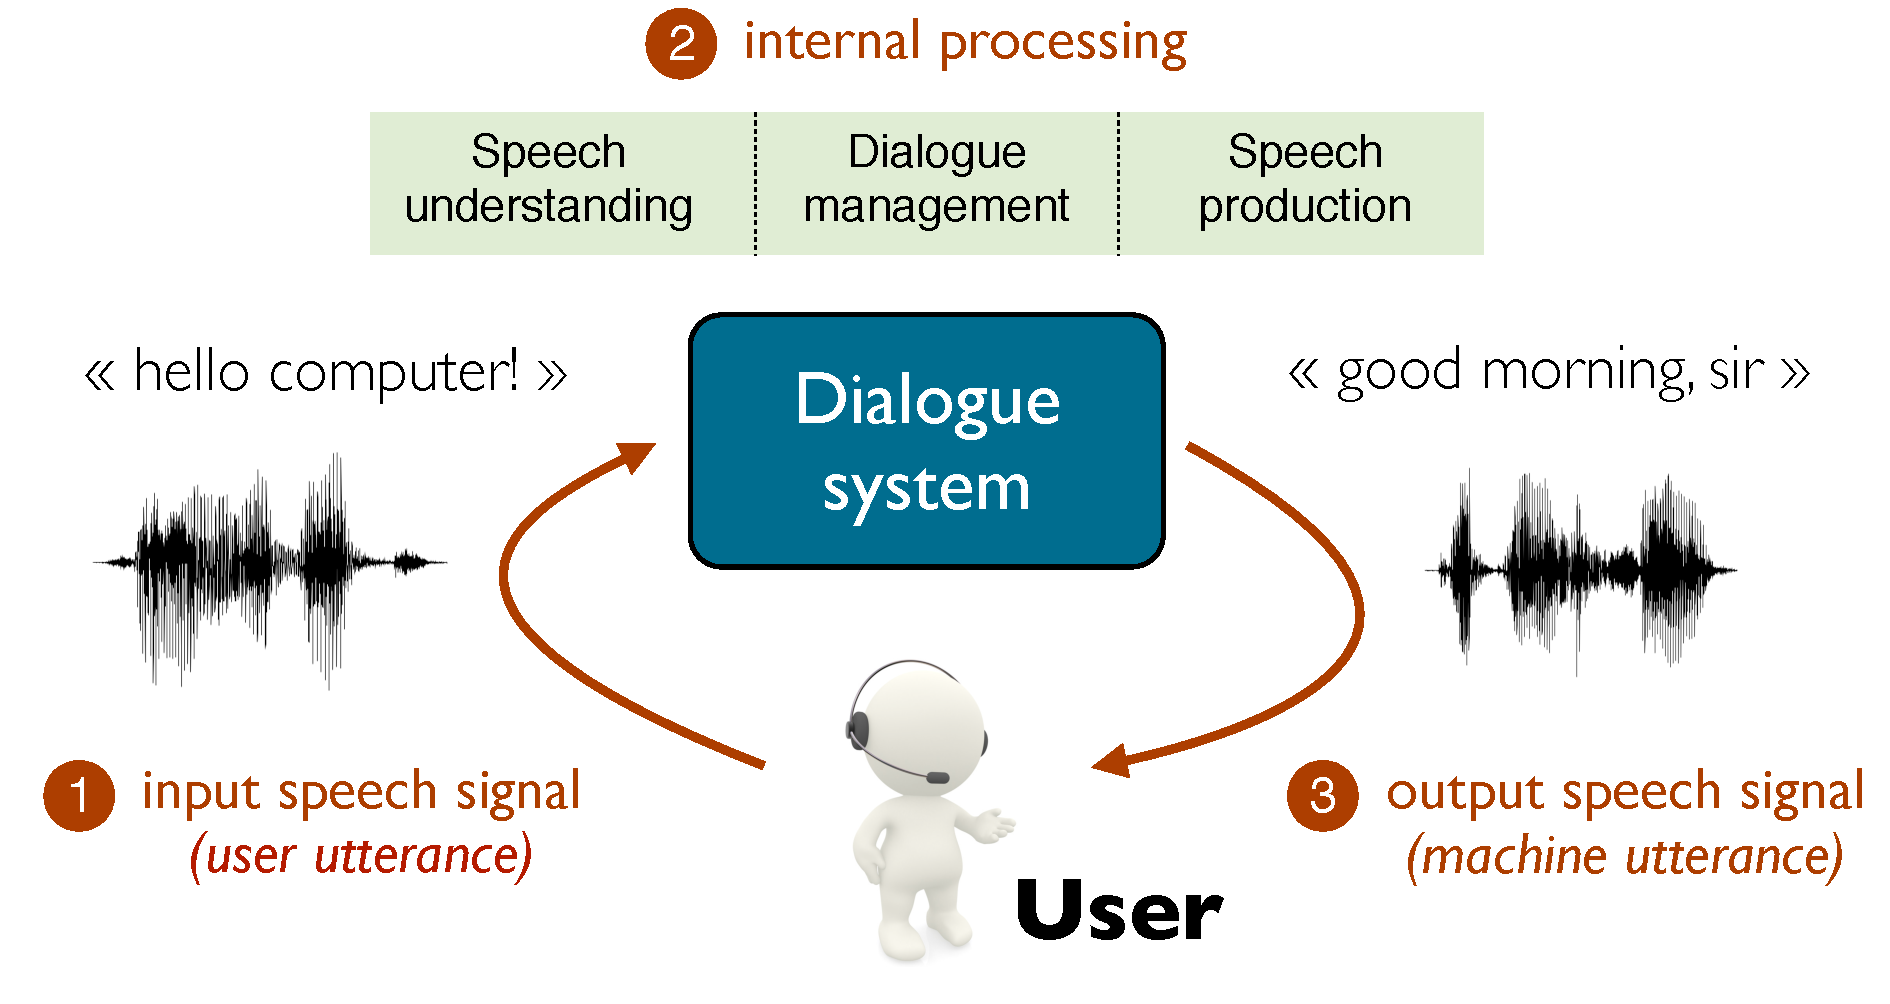
\includegraphics[scale=0.46]{imgs/basicsds.pdf}
\caption{Schematic view of a spoken dialogue system.}
\label{fig:basicsds}
\end{figure}

\section{Motivation}

Although spoken dialogue systems can greatly enhance the user interaction experience in many of today's technologies, their practical development can be a demanding enterprise. Speech is indeed much more complex than other types of (e.g.\ graphical or touch-based) user interfaces.

The present thesis concentrates on the problem of \textit{dialogue management}\index{dialogue management}.  Dialogue management is a central component in spoken dialogue systems and lies at the intersection between speech understanding and generation.  It serves a double role. Its first function is to maintain a representation of the current dialogue state\index{dialogue state}. This representation reflects the system knowledge of the current conversational situation, and often includes multiple features related to the dialogue history, the external context, and the tasks to perform.  This dialogue state is regularly updated with new information in the form of new user utterances or changes in the external context. 

The second function of dialogue management is to make decisions\index{action selection}.  Based on the current dialogue state, dialogue management must decide which actions to undertake. These actions are often communicative in nature (uttering a sentence), but can also pertain to non-verbal actions (e.g.\ waving or pointing in the case of human--robot interactions).  Dialogue management is therefore responsible for controlling the flow of the interaction, by (1) interpreting the user intentions in their context and (2) selecting which actions to perform given this context. In the example from Figure \ref{fig:basicsds}, this step corresponds to the decision of responding to the user utterance \utt{hello computer!} with another greeting action, \utt{good morning, sir}. 

Along with speech recognition, dialogue management is arguably one of the most difficult processing tasks in spoken dialogue systems. This difficulty stems from two defining characteristics of verbal interactions:
\begin{enumerate}
\item Verbal interactions are \textit{complex}.   Taking part in a dialogue requires tracking a multitude of factors, such as the interaction history, the hypothesised goals and preferences of the dialogue participants, and the external context. These factors depend on one another through multiple relations straddling the linguistic and extra-linguistic boundaries.  Selecting the action that is most appropriate in a particular situation is thus a difficult decision problem. 

\item Verbal interactions are also riddled with \textit{uncertainties}.  In order to make sense of a given dialogue, a conversational agent must handle numerous sources of uncertainty, including error-prone speech recognition, lexical,  syntactic and referential ambiguities, partially observable environments, and unpredictable interaction dynamics.  
\end{enumerate} 

The combination of these two properties forms an explosive mix.  In order to make sense of the interaction and act appropriately, the dialogue system must resort to sophisticated reasoning in order to interpret the user intentions in their context and plan the best course of action.  And it must do so under high levels of noise and uncertainty, where many pieces of information can be erroneous, missing, ambiguous, or fragmentary. This task is defined in the artificial intelligence literature as \textit{sequential decision-making under uncertainty}\index{sequential decision-making under uncertainty}, and is known to be a difficult computational problem, especially for domains as complex as spoken dialogue. Decision-making and action execution must also occur in real-time, since dialogue is by nature a real-time process. 

%\citep{Kaelbling:1998,aima2010}

Research on dialogue management can be divided into two main lines of investigation that reflect their focus on either of the two challenges we just mentioned.  

On the one hand, structural complexity is often dealt using conceptual tools borrowed from formal logic and classical planning\index{dialogue management!symbolic approaches to}.  These approaches provide principled methods for the interpretation and generation of dialogue moves through logical reasoning on the basis of a formal representation of the mental states of the dialogue participants (including their shared knowledge). Based on such representations, dialogue is then framed as a collaborative activity in which the dialogue participants work together to coordinate their actions, maintain a shared conversational context, resolve open issues and satisfy social obligations \citep{larsson2002,Jokinen:2009,Ginzburg2012}. These approaches can yield detailed analyses of various conversational behaviours, but they generally assume complete observability of the dialogue state and provide only a limited account of errors and uncertainties. In addition, they require the knowledge base on which the inference is grounded to be completely specified in advance by domain experts.  Their deployment in practical applications is therefore non-trivial. 

On the other hand, the problem of uncertainty is usually addressed by probabilistic modelling\index{probabilistic modelling} techniques \citep{Roy:2000,FramptonL09,Young:2010}.\index{dialogue management!statistical approaches to}  The state of the dialogue is here represented as a probability distribution over possible worlds.  This distribution represents the system's current knowledge of the interaction and is regularly updated as new observations are collected. These probabilistic models provide an explicit account for the various uncertainties that can arise during the interaction. They also enable the dialogue behaviour to be automatically optimised in a data-driven manner instead of relying on hand-crafted mechanisms.  Dialogue strategies can therefore be adapted to new environments or users without having to be reprogrammed. However, probabilistic models typically depend on large amounts of training data to estimate their parameters -- a requirement that is hard to satisfy for many dialogue domains.  Probabilistic models of dialogue are also usually limited to a handful of state variables and are difficult to scale to domains featuring rich conversational contexts. 

The work described in this thesis aims at reconciling these two strands of research through a new, hybrid framework to dialogue modelling and control. 

\section{Contributions}

The present thesis develops an original approach to dialogue management based on \textit{structured probabilistic modelling}.  The overarching motivation for this work is to design probabilistic models of dialogue that are scalable to rich interaction domains, yet only modest amounts of training data for their statistical optimisation.

An extensive body of work in the machine learning and decision-theoretic planning literature shows how to confront this issue by relying on more expressive representations, able to capture relevant aspects of the problem \textit{structure} in a compact manner. By taking advantage of hierarchical or relational abstractions, system designers can leverage their domain knowledge to yield probabilistic models which are both easier to learn (due to a reduced number of parameters) and more efficient to use (since the structure can be exploited by the inference algorithm).  

This thesis demonstrates how to translate these insights into dialogue modelling\index{dialogue modelling}.  The three central research questions of this thesis are:
\begin{enumerate}
\item How can we integrate prior domain knowledge into probabilistic models of dialogue?\index{dialogue management!domain knowledge in}
\item How can the parameters of these structured probabilistic models be estimated from data, using both supervised and reinforcement learning methods? \index{rule parameters!parameter estimation of} 
\item What is the empirical effect of such modelling techniques on the quality and efficiency of verbal interactions?
\end{enumerate}

\textit{Probabilistic graphical models} \citep{Koller+Friedman:09}\index{graphical models} constitute the theoretical foundations for a large part of our work.  Graphical models provide a generic, principled framework for representing and reasoning over complex probabilistic problems. They also come with well-defined data structures and general-purpose algorithms for model estimation and inference.  As shown in previous work \citep[see for instance][]{Thomson:2010:BUD:1772996.1773040}, one can elegantly represent the dialogue state as a Bayesian network\index{Bayesian network} (a well-known type of directed graphical model) factored in a set of state variables describing various aspects of the conversational situation.  The dialogue state is graphically depicted as a directed acyclic graph where the nodes correspond to particular variables and the edges are conditional dependencies between variables. To exploit such representation for decision-making tasks, the dialogue state can be extended with action and utility nodes that describe the utility for the agent of performing particular actions in a given situation. 

Statistically speaking, the estimation of such complex probabilistic structures is, however, a difficult endeavour, owing to the large number of variables and dependencies involved. The main novelty of our approach is the idea of representing the model distributions in a structured manner through the use of \textit{probabilistic rules}. \index{probabilistic rule} Probabilistic rules encode conditional distributions between variables in terms of structured mappings associating particular conditions expressed on a set of input variables to probabilistic effects on a set of output variables.  Utility distributions are also encoded in a similar manner. The conditions and effects of probabilistic rules are defined as first-order logical formulae. As new information becomes available to the dialogue manager, the Bayesian network representing the dialogue state is updated by instantiating the rules in the form of new nodes mediating between the input and output variables. Probabilistic rules are therefore employed as \textit{high-level templates} for the generation of a classical probabilistic model.  

The resulting modelling framework offers two major benefits. Most importantly, the reliance on more expressive representations can drastically reduce the number of parameters associated with the models.  Instead of being encoded through traditional probability tables, the conditional distributions between state variables are expressed through high-level rules that capture conditional dependencies with a compact set of parameters (one for each possible effect). As a consequence, these models are much easier to learn and generalise to unseen data.  In addition, the framework enables expert knowledge to be directly integrated in the probabilistic dialogue models. System developers can therefore exploit powerful abstractions to encode their prior knowledge of the dialogue domain in the form of pragmatic rules or task-specific assumptions.    
While the usefulness of domain-specific constraints has long been recognised, their use has most often been reduced to a mere external filter for classical statistical models \citep{heeman2007,williams2008}. By contrast, our approach incorporates such knowledge source in the very structure of the statistical model. 

We conducted several experiments to assess the validity of our approach in three distinct learning scenarios: \begin{enumerate} %, detailed in Section \ref{sec:wozlearning-experiments},

\item The first experiment focused on the problem of estimating action utilities given a small data set collected from Wizard-of-Oz interactions\index{Wizard-of-Oz interaction}.\footnote{A Wizard-of-Oz interaction is an experimental procedure borrowed from the field of human-computer interaction \citep{woz93}. In a Wizard-of-Oz study, the human subjects are asked to interact with a computer system that has all the appearances of reality, but is actually remotely controlled by an (unseen) human agent operating behind the curtains.  Wizard-of-Oz studies are often conducted to provide the system designers with interaction data from real users before the system is fully implemented.  The term is a cultural reference from the 1939 film ``The Wizard of Oz'' where an illusionist impersonates a powerful wizard by controlling an intimidating display from behind a curtain.}  Based on dialogue models encoded with probabilistic rules, the utilities of the different actions are learned through imitation learning. The experiment showed that the rule structure enabled the learning algorithm to converge faster and with better generalisation performance than unstructured models. This work was originally presented in \cite{rulebasedmodels-sigdial2012}. 
%, described in Section \ref{sec:rllearning-experiments},
\item The second experiment extended the above approach to reinforcement learning\index{reinforcement learning}. The goal of this study was to estimate the transition model of the domain from interactions with a user simulator. We compared the relative learning performance of two modelling approaches: one relying on unstructured distributions, and one based on probabilistic rules. The empirical results demonstrated the benefits of capturing the domain structure with probabilistic rules. The results were first published in \cite{interspeech2013}. 
\item Finally, the third and final experiment was designed to evaluate the empirical effect of the modelling framework through a user evaluation in a human--robot interaction domain. The experiment compared three alternative dialogue management methods: a purely hand-crafted approach (based on a finite-state automaton), a purely statistical approach (based on factored models) and a hybrid approach based on probabilistic rules. The rule-structured approach was shown to outperform the two baseline methods on a range of quality metrics, including both objective metrics extracted from the interaction logs and subjective metrics derived from responses to a user survey. \index{user evaluation}
\end{enumerate}

An additional contribution of this thesis is the development of a software toolkit that implements all the data structures and algorithms presented in this work. The toolkit is called \opendial{}\index{openDial@\opendial{}}  and is freely available under an open source licence.\footnote{The toolkit can be downloaded at \urlsmall{http://opendial.googlecode.com}.} The purpose of the toolkit is to enable system developers to design and evaluate dialogue systems based on probabilistic rules. All domain-specific knowledge is declaratively specified in the rules for the domain. The system architecture is therefore reduced to a small set of core algorithms for accessing and updating the dialogue state \citep{lison-semdial2012}. This architectural design makes the toolkit fully generic and domain-independent. The \opendial{} toolkit comes with a user interface allowing developers to interactively test their system and visualise how the internal dialogue state is evolving over time.  % Its implementation is described in Chapter \ref{chap:opendial}. 

We carried out all the experiments described in this thesis in a particular application domain, namely \textit{human--robot interaction} \index{human--robot interaction} (HRI).  The choice of this application domain as a test bed for our framework was motivated by two factors.  The first factor is the presence of a complex situated environment in which the agent must complete its tasks.  This dialogue context\index{dialogue context} is highly dynamic -- for instance, the physical position of objects and persons may change in the course of the interaction, and the system tasks are regularly altered as a result of the coordinated actions of the robot and human user. The second factor relates to the occurrence of multiple sources of uncertainty caused by imperfect sensory devices, unreliable motors, and failure-prone speech recognition. This combination of a rich conversational context and high levels of uncertainty is precisely the focus of the present work and justifies the selection of  human--robot interaction as a test bed to evaluate the performance of our modelling approach in real settings.

\begin{wrapfigure}[13]{r}{60mm}
\vspace{-6mm}
\centering 
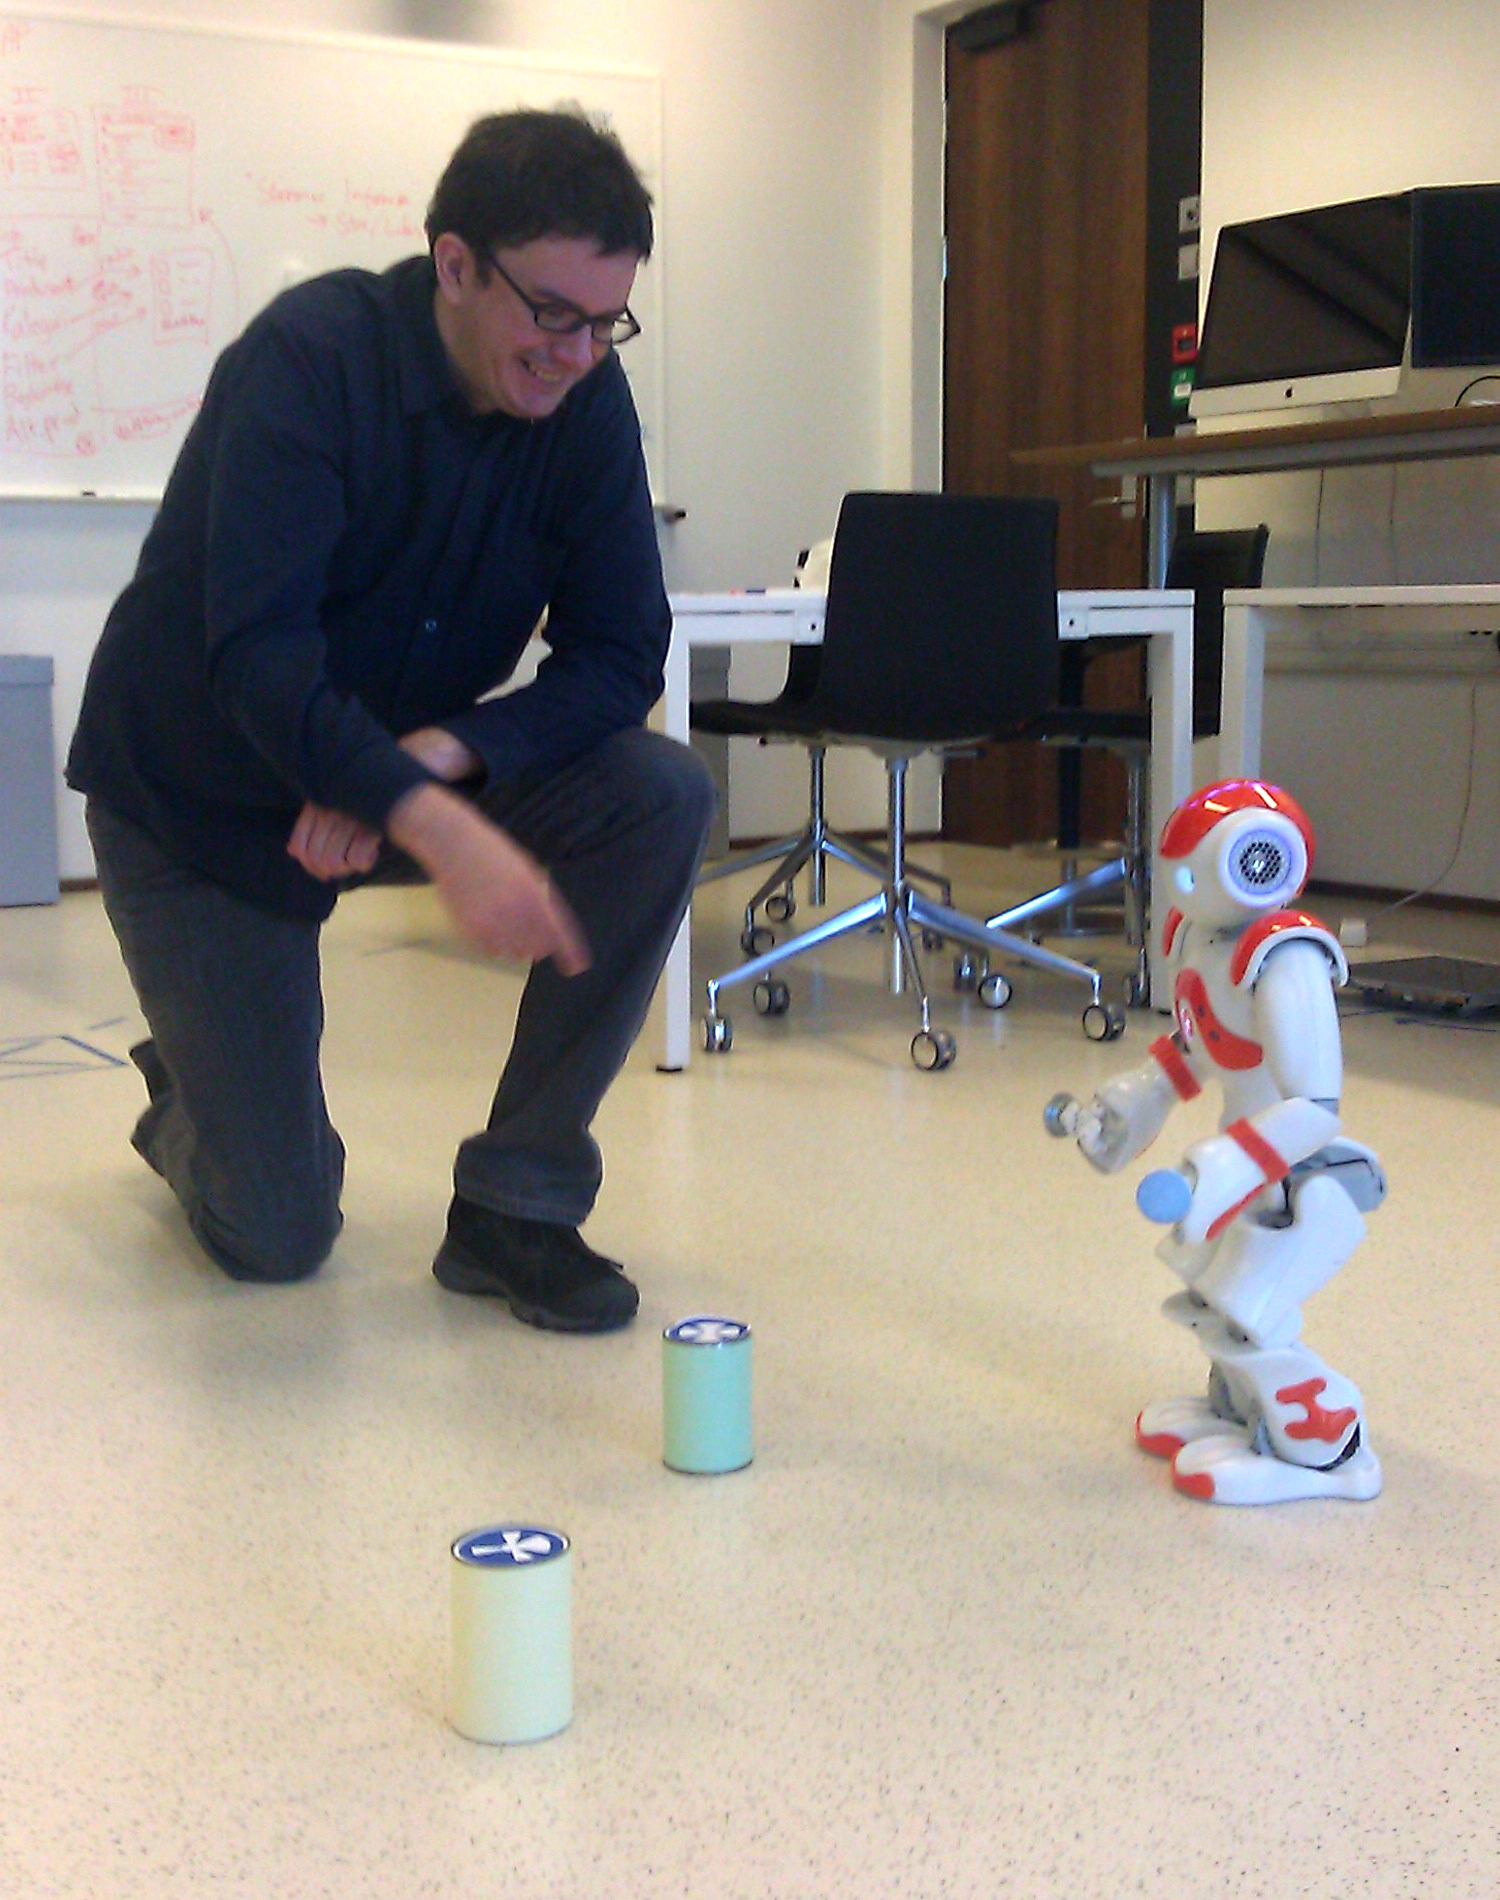
\includegraphics[scale=0.1]{imgs/nao1.jpg}
\caption{Human user interacting with the Nao robot.}
\label{fig:nao}
\end{wrapfigure}

The Nao robot V4 (NextGen) \index{Nao robot} manufactured by Aldebaran Robotics\footnote{cf.  \urlsmall{http://www.aldebaran-robotics.com}.} was used as a development and testing platform in all our experiments. An example of interaction with the robot is shown in Figure \ref{fig:nao}.  Most of our experiments involved the Nao robot conversing with a human user in a shared visual environment featuring a few basic objects that can be both perceived and grasped by the robot.  The interactions typically revolved around the completion of a few simple tasks such as moving objects from one position to another under the supervision of the human user. Chapters \ref{chap:wozlearning}--\ref{chap:user-evaluation} provide a detailed description of the interaction scenarios, data collection and evaluation setups followed for the experiments.

% combination of theory + experiments and implementation? 

\section{Outline of the thesis}

A brief overview of the thesis structure, chapter by chapter, is provided below. 

\begin{description}
  \item[\textbf{Chapter \ref{chap:background}: Background}] \hfill  \vspace{2mm}
  
This chapter introduces the fundamental concepts and methods used throughout this thesis. We start with an overview of some of the core linguistic properties of dialogue and describe key notions such as turn-taking, dialogue acts and grounding.  We then describe a range of software architectures employed to design spoken dialogue systems and the role of each component within them.  We also mention a range of important applications for spoken dialogue systems. Finally, we survey the various approaches that have been put forward in the research literature to address the dialogue management problem, including both hand-crafted and statistical methods. \vspace{2mm}

  \item[\textbf{Chapter \ref{chap:probmodelling}: Probabilistic modelling of dialogue}] \hfill \vspace{2mm}

 The chapter starts by reviewing the core notions of directed graphical models, which constitute the formal basis for our framework.  We define how Bayesian networks are constructed, and show how they can be augmented to capture temporal sequences and decision-theoretic problems. We also briefly describe the most important algorithms for learning and inference based on such models.  We then  move to the field of reinforcement learning and spell out its most central elements, such as Markov Decision Processes, value functions and policies. We also examine how reinforcement learning methods can be extended to partially observable settings, since dialogue is a prototypical example of decision-making under partial observability.  Finally, the last section translates these concepts and methods to the field of dialogue management, and discusses both supervised and reinforcement learning approaches to the optimisation of dialogue policies.
 
  \item[\textbf{Chapter \ref{chap:rules}: Probabilistic rules}] \hfill \vspace{2mm}
 
  This chapter lays down the central concepts and algorithms of our own modelling approach to dialogue management. We define what probabilistic rules are and how they are internally structured through conditions and effects.  We describe two main types of rules, used to respectively encode probability and utility distributions. We then explain how the rules are practically instantiated in the Bayesian network representing the dialogue state, as well as the algorithms employed to update the dialogue state and perform action selection. The chapter also addresses some advanced modelling questions related to the manipulation of special data structures such as lists and strings, and concludes by comparing our framework to previous work. \vspace{2mm}
  
  \item[\textbf{Chapter \ref{chap:wozlearning}: Learning from Wizard-of-Oz data}] \hfill  \vspace{2mm}
  
 This chapter shows how the parameters attached to probabilistic rules can be automatically learned from training data, in a supervised learning fashion. The algorithm used for estimating the rule parameters is grounded in Bayesian learning techniques.  To validate our approach, we detail an experiment on a statistical estimation task based on Wizard-of-Oz data collected in a human--robot interaction domain.  The experiment illustrates the benefits of probabilistic rules compared to unstructured distributions.  \vspace{2mm}

\item [\textbf{Chapter \ref{chap:rllearning}: Learning from interactions}] \hfill  \vspace{2mm}

Chapter \ref{chap:rllearning} extends parameter estimation to a reinforcement learning context.  We show how the parameters of rule-structured dialogue models can be efficiently learned from observations collected during the interaction itself, without having access to any gold standard annotations.  The procedure follows a Bayesian reinforcement learning approach and can be applied to optimise the rule parameters using both model-based and model-free variants. Finally, we report the results of two experiments carried out with a user simulator.  The experiments concentrated on the estimation of the transition model for a human--robot interaction domain, and evaluated the relative performance of a rule-structured model compared to a plain statistical model as well as the learning efficiency of model-based vs. model-free methods.   \vspace{2mm}


\item [\textbf{Chapter \ref{chap:opendial}: Implementation}] \hfill  \vspace{2mm}

Chapter \ref{chap:opendial} uncovers how the various algorithms and data structures presented in this thesis are technically integrated in the system architecture.  We explain how the \opendial{} toolkit is structured, describe how dialogue domains are practically specified in a generic XML format and discuss the implementation and performance tuning of the algorithms used for probabilistic inference and online planning.  We also compare the \opendial{} architecture to related software frameworks.  Finally, the chapter presents the integrated dialogue system employed to carry out the experiments in this thesis and the graphical user interface developed to visualise the evolution of the dialogue state over the course of the interaction. 

\item [\textbf{Chapter \ref{chap:user-evaluation}: User evaluation}] \hfill  \vspace{2mm}

This chapter presents an extensive user evaluation of our approach in a human--robot interaction domain with 37 participants.  The evaluation contrasted the empirical performance of three dialogue management strategies: a hand-crafted approach expressed as a finite-state automaton, a statistical approach based on factored models, and a hybrid approach encoded with probabilistic rules (the two latter models being estimated on the basis of a small set of Wizard-of-Oz interactions).  The empirical results show that the use of rule-structured models yields significant improvements in both objective and subjective metrics of interaction quality compared to the two baselines. \vspace{2mm}


\item [\textbf{Chapter \ref{chap:conclusions}: Concluding remarks}] \hfill  \vspace{2mm}

The final chapter concludes this dissertation with a summary of the presented research contributions, followed by an outline of future work.   \vspace{2mm}

\end{description}




\chapter{Background}
\label{chap:background}

We introduce in this chapter the most important concepts and methods employed in the field of spoken dialogue systems, with special emphasis on dialogue management.  We start by reviewing some key linguistic concepts that are particularly relevant for our work: turn-taking, dialogue acts and grounding.  A proper understanding of these aspects is indeed a prerequisite for the design of conversationally competent dialogue systems. After this linguistic overview, we move to a more technical discussion of the software architectures used to implement practical dialogue systems.  These architectures typically comprise multiple processing components, from speech recognition to understanding, dialogue management, output generation and speech synthesis.  We briefly describe the role of each component and their positions in the global processing pipeline. 

Last but not least, the final section of this background chapter delves into the diverse set of approaches that have been put forward to tackle the dialogue management problem.  We first present hand-crafted approaches, starting with finite-state policies and pursuing with more sophisticated methods based on logic- or plan-based reasoning.  Finally, we survey the more recently developed statistical approaches to dialogue management that seek to automatically extract dialogue strategies from data, based on supervised and reinforcement learning methods.

\section{What is spoken dialogue?}

We communicate in order to fulfil a wide array of social functions, such as exchanging ideas, recollecting experiences,  sustaining relationships, or collaborating with others to accomplish shared goals. These communication skills are developed in early childhood, and our cognitive abilities are in many ways shaped and amplified by this disposition for verbal interaction.  

One of the most important property of dialogue is that it is fundamentally a \textit{collaborative activity} (emphasis on both words).  It is, first of all, an \textit{activity}, which means that is is (1) motivated by the desire to achieve specific (practical or social) goals; (2) subject to costs to minimise (the communication effort); and (3) composed of a temporal sequence of basic actions.  Furthermore, if we abstract from so-called ``internal dialogues'' with oneself, dialogue involves per definition at least two participants that must act together to keep the dialogue on track.  As shown by a wealth of studies in psychology and linguistics \citep{Clark1989,Allwood92,Clark96,Garrod2004,Tomasello2005}, human conversations are characterised by a high degree of \textit{collaboration} between interlocutors.  The individuals participating in a dialogue routinely collaborate in order to coordinate their contributions and ensure mutual understanding, thereby making the interaction more efficient. This collaboration is done mostly unconsciously and is part and parcel of the conversational skills we develop as speakers of a given language. 

We describe in the next sections four major aspects of this collaborative activity: \begin{enumerate}
\item The dialogue participants take \textit{turns} in a conversation.
\item These turns are structured into basic communicative units called \textit{dialogue acts}.
\item The interpretation of these dialogue acts is subordinated to the \textit{conversational context} in which they are uttered. 
\item The participants continuously provide \textit{grounding signals} to each other in order to indicate how they understand (or fail to understand) each other's contributions.
\end{enumerate}

\subsection{Turn-taking}

Turn-taking\index{turn-taking} is one of the most basic (yet often neglected) aspect of spoken dialogue. The physical constraints of the communication channel impose that participants take turns in order to speak.   Turn-taking is essentially a resource allocation problem.  In this case, the resource to allocate is called the \textit{conversational floor}\index{conversational floor}, and social conventions dictate how the dialogue participants are to take and release their turns. 

The field of  \textit{conversation analysis}\index{conversation analysis} studies what these conventions are and how they combine to shape conversational behaviours. Human conversations are indeed remarkably efficient at turn-taking.  Empirical cross-linguistic studies have shown that the average transition time between turns revolves around 250 ms. \citep{Stivers30062009}.\footnote{Interestingly, this duration is shorter than the time required for a human speaker to plan the motor routines associated with the physical act of speaking.  This means that the next speaker must start planning his utterance before the current turn is complete, and predict when a potential turn boundary is likely to appear.} In addition, most of the utterances do not overlap: \cite{Levinson1983} indicates that less than 5 \% of the speech stream contains some form of overlap in spontaneous conversations.  

A wide variety of cues are used to detect turn boundaries, such as silence, hesitation markers, syntax (complete grammatical unit), intonation (rising or falling pitch) and body language, as described by \cite{Duncan1972}.   These cues can occur jointly or in isolation. Upon reaching a turn boundary, a set of social conventions governs who is allowed to take the turn.  The current speaker can explicitly select the next person to take the turn, for instance when greeting someone or asking a directed question \citep{sacks1974}.   This selection can also occur via other mechanisms such as gaze.  When no such selection is indicated, other participants are allowed to take the turn.  Alternatively, the current speaker can continue to hold the floor until the next boundary. 

Turn-taking is closely related to the notion of \textit{initiative}\index{initiative} in human--computer interaction. The vast majority of dialogue systems currently deployed are either system-initiated or user-initiated.  In a system-initiated dialogue, the dialogue system has full control on how the interaction is unfolding -- i.e. the system is asking all the questions and waiting for the user responses.  A user-initiated dialogue is the exact opposite: in such settings, the user is assumed to lead the interaction and request information from the system.  The most complex -- but also most natural -- interaction style is the mixed-initiative\index{mixed initiative}, where both the user and the dialogue system are allowed to take the initiative at any time and decide to either provide or solicit information whenever they see fit \citep{Horvitz:1999}. 

The turn-taking behaviour of most current-day dialogue systems remains quite rudimentary.  The most common method to detect the end of a user turn is to wait for a silence longer than a manually fixed threshold, typically ranging between 
\textonehalf  $ $ and 1.0 second.  Some system architectures also include routines for handling barge-ins\index{barge-in} -- that is, user interruptions --  \citep{StromS00}, while others simply ignore them altogether. Turn-taking has recently become a focus of research in its own right in the dialogue system literature \citep{RauxE09,Gravano2011}, in an effort to break away from the ping-pong interaction style that characterises most current dialogue interfaces.  

\subsection{Dialogue acts}

Each turn is constituted of one or more utterances.  As argued by \cite{Austin1962} and \cite{Searle1969}, utterances are nearly always purposeful: they have specific goals and are intended to provoke a specific psychological effect on the listener(s).  They are therefore best described as actions rather than abstract statements about the world.  The notion of dialogue act\index{dialogue act} embodies precisely this idea.\footnote{Dialogue acts have gone through multiple names over time, owing to the diverse range of research fields that have studied them, from philosophy to descriptive and computational linguistics.  As listed in \cite{mctear2004}, alternative denominations include speech acts \citep{Searle1969}, communicative acts \citep{allwood1976}, conversation acts \citep{TraumH92}, conversational moves \citep{sinclair1975}, and dialogue moves \citep{LarssonCEL99}.} \cite{Bunt1996} defines a dialogue act as a ``functional unit of a dialogue used by the speaker to change the context''.

In his seminal work on the philosophy of language, \cite{Searle1979} established a taxonomy of speech acts\index{speech act} divided in five central categories:
\begin{description}
\item[Assertives: ] Committing the speaker to the truth of a proposition. \\
Examples: \utt{I swear I saw him on the crime scene.}, \utt{I bought more coffee.}
\item[Directives: ]  Attempts by the speaker to get the addressee to do something. \\ Examples:  \utt{Clean your room!}, \utt{Could you post this for me?}
\item[Commissives: ] Committing the speaker to some future course of action. \\ Examples: \utt{I will deliver this review before Monday.}, \utt{I promise to work on this.}
\item[Expressives: ] Expressing the psychological state of the speaker about a state of affairs. \\ Examples: \utt{I am so happy for you!}, \utt{Apologies for being late.}
\item[Declaratives: ] Bringing about a different state of the world by the utterance. \\ Examples: \utt{You're fired.}, \utt{We decided to let you pass this exam.}
\end{description}

Modern taxonomies of dialogue acts are significantly more detailed than the one introduced by Searle.  They also provide detailed accounts of various dialogue-level phenomena such as grounding (cf. next section) that were absent from Searle's analysis. The most well-known annotation scheme is DAMSL (Dialogue Act Markup in Several Layers\index{DAMSL}) and was initially formalised by \cite{Core1997}.  DAMSL defines a rich, multi-layered annotation scheme for dialogue acts that is both domain- and task- independent.  A modified version of this scheme was applied to annotate the Switchboard corpus\footnote{The Switchboard corpus is a corpus of spontaneous telephone conversations collected in the early 1990's.  It includes about 2430 conversations averaging 6 minutes in length; totalling over 240 hours of recorded speech with native speakers of American English \citep{Godfrey1992}.} based on a set of 42 distinct dialogue acts \citep{Jurafsky1997}, including greeting and closing actions, acknowledgements, clarification requests, self-talk, responses, and many more.  An interesting aspect of DAMSL is the use of two complementary dimensions in the markup: the \textit{forward-looking functions}\index{forward-looking function}, which are the traditional speech acts in Searle's sense (assertions, directives, information requests, etc.) and the \textit{backward-looking functions}\index{backward-looking function} that respond back to a previous dialogue act and can signal agreement, understanding, or provide answers.  Both backward- and forward-looking functions can be present in the same utterance. 

Determining the dialogue act corresponding to a given utterance is a non-trivial operation. The type of utterance only gives a partial indication of the underlying dialogue act -- a question can for instance express a directive (\utt{Could you post this for me?}).  In order to accurately classify a dialogue act, a variety of linguistic factors must be taken into account, such as prosody, lexical, syntactic and semantic features, and the preceding dialogue history \citep{jurafsky1998,Shriberg1998,stolcke2000,Keizer2007}.

\subsection{Interpretation of dialogue acts} 

Dialogue acts are strongly contextual in nature: their precise meaning can often only be comprehended within the particular conversational context in which they appear. The successful interpretation  of dialogue acts must therefore venture beyond the boundaries of the isolated utterance. We briefly review here three striking aspects of this dependence on context.

\subsubsection*{Implicatures}
\index{implicature}
As shown by \cite{Grice1989}, an important part of the semantics of dialogue acts is not explicitly stated but rather implied from the context.  Consider the following constructed example: 
\begin{center}
\begin{dialogue}
\speak{A} Is William working today?
\speak {B} He has a cold.
\end{dialogue}
\end{center}
In order to retrieve the ``suggested'' meaning behind B's utterance -- namely, that William is probably not working --, one needs to assume that B is cooperative and that his response is therefore relevant to A's question.  If an utterance initially seems to deliberately violate this principle, the listener must search for additional hypotheses required to make sense of the dialogue act. \cite{Grice1989} formalised these ideas in terms of a cooperative principle composed of four conversational maxims that are assumed to hold in a natural conversation: the maxim of quality (``be truthful''), the maxim of quantity (``be exactly as informative as required''), the maxim of relation (``be relevant'') , and the maxim of manner (``be relevant'').  These notions have been further developed by various theorists such as \cite{wilson2002relevance} and \cite{horn2008handbook}.  A computational account of these implicatures (and application to dialogue systems) is provided by \cite{benotti2010implicature}. 


\subsubsection*{Non-sentential utterances}
\label{non-sentential utterance}
\index{non-sentential utterance}
Non-sentential (also called elliptical) utterances are linguistic constructions that lack an overt predicate.  They include expressions such as  \utt{where?}, \utt{at 8 o'clock}, \utt{a bit less, thanks} and \utt{brilliant!}. Their interpretation generally requires access to the recent dialogue history to recover their intended meaning. This can lead to ambiguities in the resolution, as illustrated in these examples modified from \cite{Fernandez:2007}: \begin{itemize}
\item A: ``When do they open the new station?''  $\rightarrow$ B: ``Tomorrow'' (\textit{short answer})
\item A: ``They open the station today''  $\rightarrow$ B: ``Tomorrow'' (\textit{correction})
\item A: ``They open the station tomorrow''  $\rightarrow$ B: ``Tomorrow'' (\textit{acknowledgement})
\end{itemize}

Various accounts of non-sentential utterances have been proposed, based on e.g. discourse coherence \citep{Schlangen03theinterpretation} or interaction-oriented semantics \citep{fernandez2006non,Ginzburg2012}. Machine learning approaches have also been developed \citep{Schlangen:2005,Fernandez:2007}. 

\subsubsection*{Referring expressions}

Finally, dialogue acts are replete with linguistic expressions that refer to some aspect of the conversational context.  These references can be either deictic or anaphoric. 

A deictic marker\index{deictic marker} is a reference to an entity that is determined by the context of enunciation.  Examples of such markers are \utt{here} (spatial reference), \utt{yesterday} (temporal reference), \utt{this mug} (demonstrative), \utt{you} (reference to a person), or even pointing gestures. By their very definitions, deictic markers refer to different realities depending on the situation in which they are used: a \utt{here} uttered in a classroom differs from a \utt{here} uttered in the countryside.  

In addition, dialogue can also include anaphoric expressions -- that is, expressions that refer to an element that has been previously mentioned through the history of the dialogue. An simple example of such anaphoric expression can be seen in the question-answer pair \utt{Is William working today?} $\rightarrow$ \utt{He has a cold}, where the pronoun \utt{he} must be resolved to \utt{William}. 

The appropriate processing of deictic and anaphoric expressions is an important question in dialogue systems, and pertains both to the interpretation and production process. Multiple approaches have been pursued, relying on symbolic \citep{Eckert2000} or statistical techniques \citep{StrubeM03,Stent2010}.  Researchers have also investigated the integration of salience measures \citep{Kelleher:2004}, multimodal cues \citep{Frampton:2009,Chen:2011}, the processing of spatial referring expressions \citep{zender/etal:2009-ijcai} and the incrementality of the resolution process \citep{schlangen2009incremental,poesio2011incremental}. 

\subsection{Grounding}

Dialogue acts are executed as part of a larger collaborative activity that requires the active coordination of all conversational partners, i.e. speaker(s) as well as hearer(s).  This coordination takes place at various levels.  The first and most visible level is the content of the conversational activity.   The partners must ensure mutual understanding of each other's contribution, to control that they remain ``on the same page''.  In addition, they  also coordinate the process by which the conversational activity moves forward -- by signalling that they are attending to the person who currently holds the conversational floor and acknowledging her/his contributions to the dialogue.

As an illustration, consider this short excerpt from a conversation transcribed in the British National Corpus \citep{bnc} :

\begin{dialogue} 
\speak{Kathleen } How come they can take time off yet you can't?
\speak{Steve } $\ \ \ \ \ \ $ He's been there longer than me.
\speak{Kathleen } Oh.
\speak{Steve }  $\ \ \ \ \ \ $ I can, I might have two holidays now, two days' holiday. ...
\speak{Kathleen } Well ... I don't get that, me.
\speak{Steve }  $\ \ \ \ \ \ $ What?
\speak{Kathleen } All these two days' holiday and this, you've had Christmas.
\speak{Steve }  $\ \ \ \ \ \ $ You get two point summat\footnote{``Summat'' is slang for ``something'' in the Yorkshire region. } days per month worked
\speak{Kathleen } Oh so you should've got them for January? ...
\speak{Steve }  $\ \ \ \ \ \ $ right?
\speak{Kathleen } Yeah.
\speak{Steve }  $\ \ \ \ \ \ $ And I worked three month before Christmas so I got six point summat days
\speak{Kathleen } For Christmas.
\speak{Steve }  $\ \ \ \ \ \ $ so then I had all Christmas off.
\speak{Kathleen } Oh! \\
 $\phantom{a} \ \ \ \ \ \ \ $ Yeah I get it now. \\
 $\phantom{a} \ \ \ \ \ \ \ $ ... I thought you got Christmas off like we got Christmas off.
\speak{Steve }  $\ \ \ \ \ \ $ No. \\ 
 $\phantom{a} \ \ \ \ \ \ \ $ You gotta earn them. ... \vspace{-2mm}
 \begin{flushright}\begin{scriptsize}(\urlsmall{http://www.phon.ox.ac.uk/SpokenBNCdata/KCX.html})\end{scriptsize}\end{flushright} 
\end{dialogue} 

We can observe in this short dialogue that the interlocutors constantly rely on the \textit{common ground} of the interaction to move the dialogue forward.  They regularly check what pieces of information are mutually known and understood (e.g. \utt{right?}).  They also make use of a variety of signals to indicate when things are properly grounded (\utt{oh}, \utt{yeah}, \utt{I get it}) and when they are not (\utt{I don't get that}, \utt{what?}). The common ground\index{common ground} progressively expands as the dialogue unfolds -- for instance, the system of holiday entitlement is not initially part of the shared knowledge for both speakers at the onset of the conversation, but becomes so towards the end. 

The common ground is defined as the collection of shared knowledge, beliefs and assumptions that is established during an interaction.\footnote{An information that is part of the common ground for a given group is more than simply known by every member of the group.  All group members must also be aware that the information is shared and known by the other members. Formally speaking, a proposition $p$ is part of the common knowledge for a group of agents $G$ when all the agents in $G$ know $p$, and they also all know that they all know $p$, and they all know that they all know that they all know $p$, \textit{ad infinitum}. This definition can be formalised using the mathematical apparatus of set theory or epistemic logic \citep{meyer2004epistemic}. } Each dialogue act is built upon the current common ground and participates in its gradual expansion and refinement.  This process is called \textit{grounding}\index{grounding}.  A variety of feedback mechanisms  can be used to this effect.  As described by \cite{Clark1989}, positive evidence\index{positive feedback} of understanding can be expressed via cues such as:
\begin{description}
\item[Continued attention: ] The hearer shows that he/she continues to attend to the speaker.
\item[Relevant next contribution: ] The hearer produces a relevant follow-up, as in the answer \utt{He's been there longer than me} following the question that precedes it.
\item [Acknowledgement: ] The hearer nods or utters a backchannel such as \utt{mm}, \utt{uh-uh}, \utt{yeah}, or an assessment such as \utt{I see}, \utt{great}, \utt{I get it now}.
\item [Demonstration: ] The hearer demonstrates evidence of understanding by reformulating or completing the speaker utterance.
\item [Display: ] The hearer reuses part of the previous utterance.
\end{description}

Communication problems can also occur, owing to e.g. misheard or misunderstood utterances. The hearer should in this case provide negative feedback to signal trouble in understanding. A large panel of clarification and repair strategies\index{clarification strategy} \index{repair strategy} are available to recover from these communicative failures.  These strategies include backchannels\index{backchannel} (\utt{mm?}), confirmations  (\utt{Do you mean that...?}), requests for disambiguations, invitations to repeat, and tentative corrections.  

All in all, these positive and negative signals enable the dialogue participants to dynamically synchronise what the speaker intends to express and what the hearers actually understand.   This grounding process operates mostly automatically, without deliberate effort.  It is closely related to the concept of interactive alignment\index{alignment} that has recently been articulated by \cite{Garrod2004,Garrod2009}. Humans show a clear tendency to (unconsciously) imitate their conversational partners. In particular, they automatically align their choice of words, a phenomenon called lexical entrainment\index{lexical entrainment} \citep{brennan1996conceptual}.  But alignment also occurs on several other levels such as grammatical constructions \citep{branigan2000syntactic}, pronunciation \citep{pardo2006phonetic}, accents and speech rate \citep{giles19911}, and even gestures and facial expressions \citep{bavelas1986show}.  

A proper treatment of grounding is critical for the development of conversational interfaces.  As already mentioned in the introductory chapter, comprehension errors are indeed ubiquitous in spoken dialogue systems.  The potential sources of misunderstandings are abundant, from error-prone speech recognition to out-of-domain utterances, unresolved ambiguities, and unexpected user behaviour.  Appropriate grounding strategies are crucial to address these pitfalls. Grounding for dialogue systems is an active area of research and important advances have been made regarding the formalisation of rich computational models of grounding \citep{Traum:1994thesis,MathesonPT00}, the generation of clarification requests \citep{Purver04Thesis,Rieser:2005}, the design of human-inspired error handling\index{error handling} strategies \citep{Skantze2007}, the integration of non-verbal cues such as gaze, head nods and attentional focus \citep{Nakano:2003} and the development of incremental grounding mechanisms \citep{visser_toward_2012}.

\section{Spoken dialogue systems}
\label{sec:sds}
After reviewing some of the core properties of human dialogues, we now discuss how to develop practical computer systems that aim to emulate such type of conversational behaviour.   In the introduction chapter, Figure \ref{fig:basicsds} represented a dialogue system as a black box taking speech inputs from the user and generating spoken responses.  Real-world dialogue systems have however a complex internal structure, as we detail in the next pages.

 \subsection{Architectures}
\label{sec:architectures}

Spoken dialogue systems (SDS) often take the form of complex software architectures\index{dialogue system architectures} that encompass a wide range of interconnected components. These components are dedicated to various tasks related to speech processing, understanding, reasoning and decision-making. These tasks can be grouped into five major components: 
\begin{enumerate}
\item \textit{Speech recognition}, in charge of mapping the raw speech signal to a set of recognition hypotheses for the user utterance(s).
\item \textit{Natural language understanding}, in charge of mapping the recognition hypotheses to high-level semantic representations of the dialogue act performed by the user.
\item \textit{Dialogue management}, in charge of interpreting the purpose of the dialogue act in the larger conversational context and deciding what communicative action to perform (if any).
\item \textit{Natural language generation}, in charge of finding the best linguistic (and extra-linguistic) realization for the selected communicative action.
\item And finally, \textit{text-to-speech synthesis}, in charge of synthesizing an audio signal out of the generated utterance.
 \end{enumerate}
 \index{speech recognition}\index{dialogue understanding}\index{dialogue management}\index{natural language generation}\index{text-to-speech synthesis}
 
 Figure \ref{fig:architecture} shows the flow of information for a prototypical spoken dialogue system. Many systems rely on additional middleware to act as a ``software glue'' between the components and handle the information exchange and scheduling of modules \citep{jaspis2004,Herzog:2004,Bohus:2009,schlangen2010}.
   
 \begin{figure}[h]
\centering
\vspace{5mm}
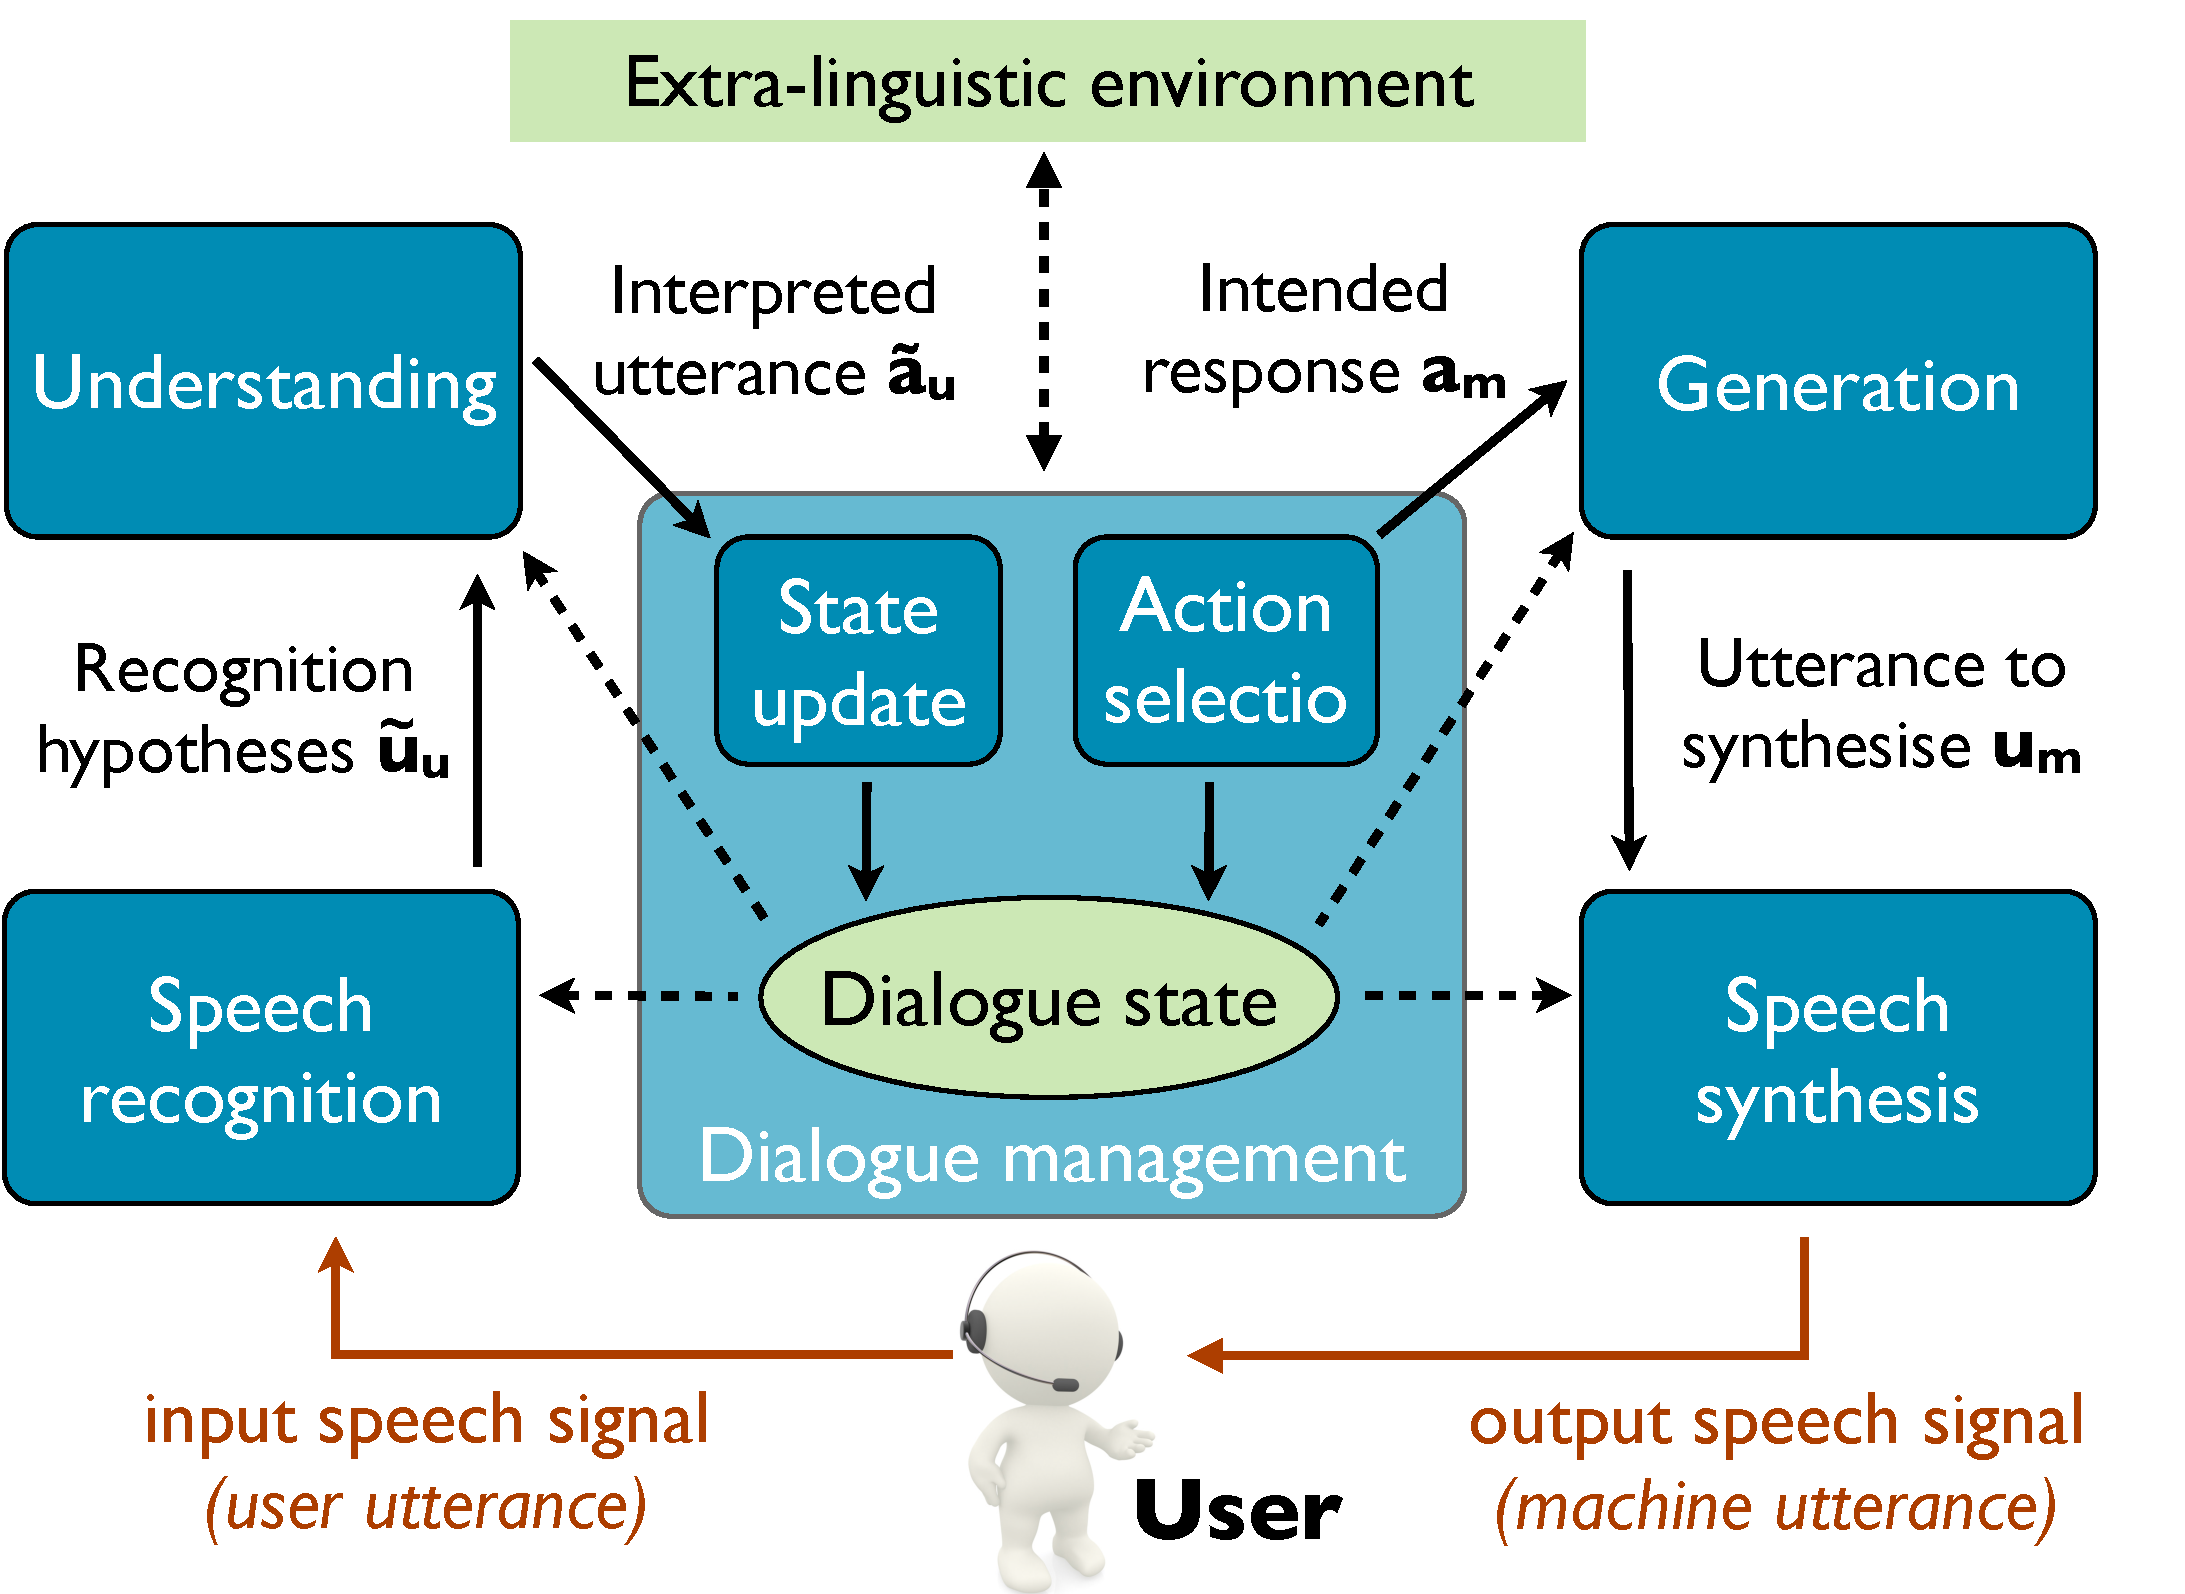
\includegraphics[scale=0.30]{imgs/architecture.pdf}
\vspace{5mm}
\caption{Information flow for a typical spoken dialogue system. The solid lines denote necessary input and outputs while the dotted lines represent optional contextual information.}
\label{fig:architecture}
\end{figure}

Spoken dialogue systems can use other modalities than speech.  In particular, additional communication channels such as touch, gestures, gaze, and other body movements can be fruitfully exploited.  As shown by e.g. \cite{smartkom}, multiple modalities can be employed to enrich communication in both directions (understanding and generation). \index{multi-modality}\index{multi-modal dialogue system}In particular, the system can refine its understanding of the actual user intentions by fusing information perceived through multiple information channels such as gestures \citep{stiefelhagen2004} or gaze \citep{koller2012}.  Non-verbal modalities can also be put to use to enhance how information is presented back to the user and convey additional grounding signals, through e.g. facial expressions and gestures. The use of multiple modalities can notably reduce understanding errors and cognitive load \citep{oviatt2004we} as well as improve the overall user experience \citep{JokinenH06}.  For all their advantages, multimodal architectures pose however a number of additional challenges related to timing, synchronisation \citep{DBLP:conf/hri/SalemKJ13} and increased system complexity. 

In addition to these non-verbal modalities, many dialogue domains are also grounded in an external context that must be accounted for\index{contextual awareness}\index{contextual modelling}.  This external context might be a physical environment for human-robot interaction, a virtual world for embodied virtual agents, a spatial location for in-car navigation systems, or simply a database of factual knowledge for information systems. Contextual factors of relevance for the application must be continuously monitored by the dialogue system (and updated whenever necessary), as many components depend on the availability of such context model for their internal processing.  Furthermore, the agent can often actively influence this context through external actions -- for instance, a grasping action will modify the location of the gripped object.   This contextual awareness necessitates the integration of additional functionalities for perception and actuation. In human--robot interaction\index{human--robot interaction} domains, these extra-linguistic modules can notably include subsystems for object and scene recognition, spatial navigation, and various motor routines for locomotion and manipulation  \citep{1570637,goodrich2007human,HawesSWZJKBBS07}. 

Several types of architectures have been proposed to assemble these components in a unified framework.  The simplest approach is to arrange the components sequentially in a pipeline\index{pipeline architecture} starting from speech recognition and ending with speech synthesis.  This approach, although relatively straightforward to develop, suffers from a number of shortcomings, amongst which the rigidity of the information flow and the difficulty of inserting feedback loops between components. Pipelines also offer poor turn-taking capabilities, since the system is unable to react before the pipeline has been fully traversed \citep{RauxE09}. More advanced architectures -- including the one put forward in this thesis -- are based on the notion of \textit{information state}\index{information state} \citep{larsson2000information,Bos2003}.  These approaches are essentially blackboard architectures revolving around a central dialogue state that is read and written by various modules connected to it.  These modules monitor the state for relevant changes, in which case they trigger their processing routines and update the state with the result.  The main advantages of such architectures are (1) a more flexible information flow, since the modules are allowed to process and update information in any order, and (2) the possibility to define modules that take full advantage of the contextual information encoded in the dialogue state.  Figure \ref{fig:architecture_comp} provides a graphical illustration of the difference between pipeline and information-state-based architectures.  

 \begin{figure}[h!]
\centering
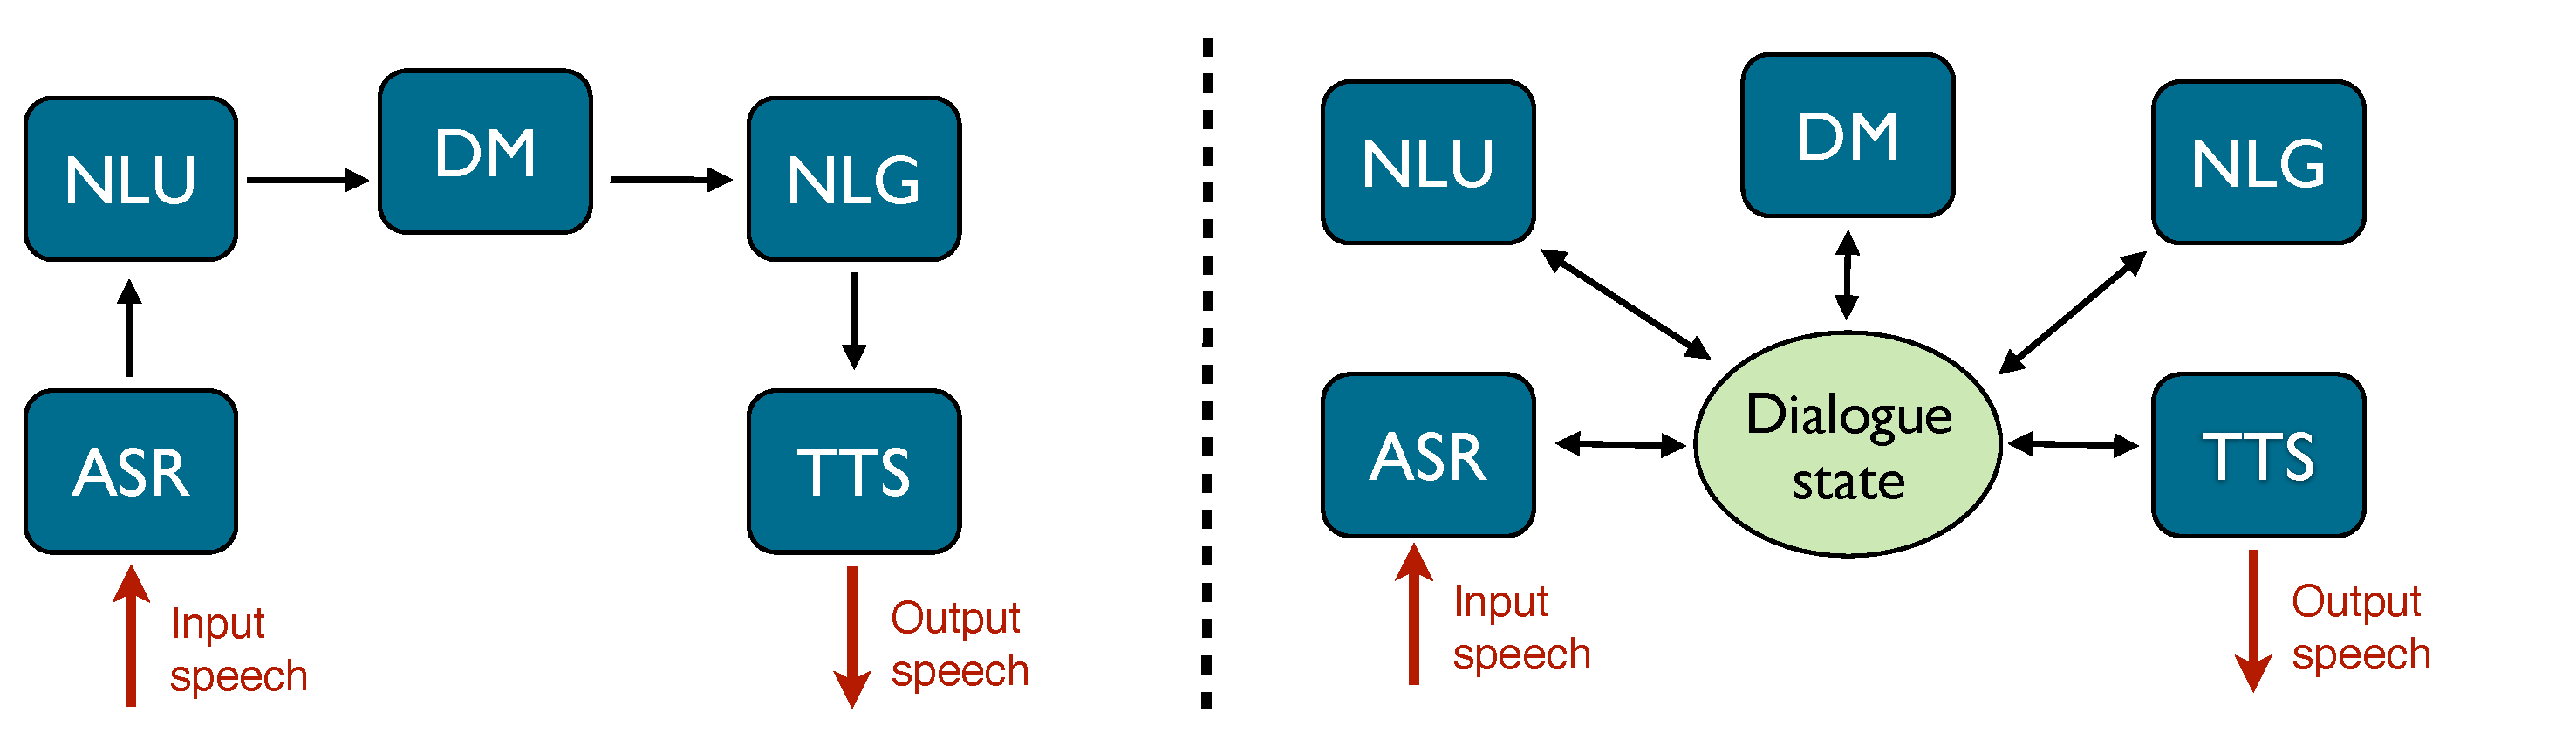
\includegraphics[scale=0.28]{imgs/architecture_comparison.pdf}
\caption{Comparison between pipeline (left) and information state (right) system architectures.   ASR = \textit{Automatic Speech Recognition}, NLU = \textit{Natural Language Understanding}, DM = \textit{Dialogue Management}, NLG = \textit{Natural Language Generation}, and TTS =\textit{Text-to-Speech Synthesis}.}
\label{fig:architecture_comp}
\end{figure}

Finally, a last aspect of dialogue system architectures that has been subject to recent research pertains to \textit{incremental processing}.  Many dialogue architectures must wait for an utterance to be fully pronounced to start its interpretation and decide on subsequent actions.  This workflow usually leads to poor reactivity and unnatural conversational behaviours.  To address this shortcoming, new architectures have been proposed to integrate incremental processing at various stages of interpretation and decision-making \citep{schlangen2009general}.\index{incremental processing}


\subsection{Components}

As explained in the previous section, the components of a dialogue systems can typically be grouped in five major steps.  We briefly describe here the role of these components and define their respective inputs and outputs.

\subsubsection*{Speech recognition}
\index{speech recognition}
Upon detection of a new speech signal emanating from the user, the first task is to recognise the corresponding utterance. Speech recognition is responsible for converting the raw speech signal from the microphone(s) into a set of hypotheses $\tilde{u}_u$ representing the words uttered by the user. To this end, the speech signal is first converted into a digital format and split into short frames (usually 10 ms). A set of acoustic features is then extracted for each frame using signal processing techniques.  Once these acoustic features are extracted, two statistical models are combined to estimate the most likely recognition hypotheses: the \textit{acoustic model} and the \textit{language model}.  \index{acoustic model}\index{language model}

The acoustic model defines the observation likelihood of particular acoustic features for a given phone\footnote{A phone is an individual sound unit of speech.  Technically speaking, acoustic models are not defined over entire phones but over sub-segments, typically decomposed into three parts: beginning, middle and end.}, while the language model defines the probability of a given sequence of words. This distinction rests on the formalisation of the speech recognition task as a \textit{Hidden Markov Model} (HMM)\index{Hidden Markov Model}, where the states represent the sequence of phones, and the observations are the acoustic features.  

%Given a sequence of acoustic observations $O$, the probability of a word sequence $W$ is straightforwardly derived using Bayes' rule: 
%\begin{equation}
%P(W|O) = \frac{P(O|W) P(W)}{P(O)} 
%\end{equation}
%where $P(O|W)$ is encoded by the acoustic model and $P(W)$ by the language model. $P(O)$ is a normalisation factor that can be ignored for decoding purposes. 

For the practical development of spoken dialogue systems, the most important element of a speech recogniser is the language model.  The language model effectively represents the set of utterances that can be accepted as inputs to the system (and their relative probabilities).  The model can be encoded either in the form of a hand-crafted recognition grammar, or via statistical modelling based on a particular corpus of reference.  In the latter case, the language model typically takes the form of an N-gram model, often a bi- or tri-gram corrected with appropriate smoothing and back-off techniques  \citep{Jelinek:1998,ChenG99}.  It is also often beneficial to dynamically modify the language model at runtime to reflect the changing context and dialogue state.  This real-time model adaptation can notably be realised by priming the words or expressions that are most contextually relevant \citep{gruenstein2005context,ESSLLI2008-springerreprint}.

The output of the speech recogniser is typically a N-best list\index{N-best list} (or recognition lattice) representing a set of possible hypotheses for the utterance, together with their relative confidence score or probabilities.  Thus, the output of the speech recogniser is a list expressed as: 
\begin{equation*}
\tilde{u}_u = \langle (\tilde{u}_u^{(1)}, p^{(1)}), (\tilde{u}_u^{(2)}, p^{(2)}), ... (\tilde{u}_u^{(n)}, p^{(n)})\rangle
\end{equation*}
where $\tilde{u}_u^{(i)}$ represents a specific recognition hypothesis and $p^{(i)}$ its corresponding probability.\footnote{In order to be proper probabilities,  the usual axioms $0 \leq p^{(i)} \leq 1$ for all $p^{(i)}$ and $\sum_{i=1}^n p^{(i)} = 1$ must be satisfied.   It should also be noted that in practice, many speech recognisers only provide raw confidence scores for their hypotheses.  Estimating the exact correspondence between these scores and meaningful probabilities is a non-trivial task that has been investigated by e.g. \cite{Williams08}.} 

\subsubsection*{Natural language understanding}
\label{section:speechunderstanding}

Once the recognition hypotheses for the utterance have been generated by the speech recogniser, the next task is to extract its semantic content.  The goal of natural language understanding (NLU) is to build a representation of the meaning(s) expressed by the form of a given utterance.  This task is a notoriously difficult endeavour, due to the combination of various factors. The first difficulty lies in speech recognition errors, with WER (Word Error Rates) often revolving around 20 \% for many dialogue applications.  The syntactic and semantic analysis of utterances is likewise complicated by the occurrence of sentential fragments,  disfluencies of various sorts (e.g. filled pauses, repetitions, corrections) and ambiguities\index{ambiguities} that must be resolved at multiple linguistic levels. 

Natural language understanding can be decomposed in a number of steps.  Parsing corresponds to the task of extracting the syntactic structure of the utterance and mapping it to a semantic representation.  Spoken language parsing can be realised through various techniques, from keyword or concept spotting \citep{KomataniTKK01,ZhangZY07} to shallow semantic parsing \citep{Coppola:2009}, grammar-based parsing \citep{VanNoord1999} and statistical parsing \citep{He200585}.  It has been shown useful to apply upstream preprocessing techniques to correct speech recognition errors \citep{Ringger:1996} and filter out disfluencies \citep{Johnson:2004}. In addition, referring expressions might also need to be resolved \citep{Funakoshi:2012}.  Finally, the dialogue act associated with the utterance must be determined \citep{stolcke2000,Keizer2007}. \cite{demori2008} provides a survey of the various models and techniques used in the field of spoken language understanding. 

Given speech recognition hypotheses $\tilde{u}_u$ given as inputs, and possibly a representation of the dialogue history and external context, the task of natural language understanding is to extract a corresponding N-best list of dialogue act hypotheses $\tilde{a}_u$ defined as: \begin{equation*}
\tilde{a}_u = \langle (\tilde{a}_u^{(1)}, p^{(1)}), (\tilde{a}_u^{(2)}, p^{(2)}), ... (\tilde{a}_u^{(n)}, p^{(n)})\rangle
\end{equation*}
where $\tilde{a}_u^{(i)}$ represents a dialogue act hypothesis, usually represented in a logical form with various predicates and arguments, and $p^{(i)}$ its corresponding probability.

\subsubsection*{Dialogue management}
\index{dialogue management}

Dialogue management occupies a central stage in spoken dialogue systems.  As already mentioned in the introductory chapter, dialogue management serves a double role.  The first task of the dialogue manager is to maintain a representation of the current dialogue state\index{dialogue state} and update it as new information becomes available\index{dialogue state update}.\footnote{Some approaches explicitly distinguish between two types of management tasks: task management, responsible for monitoring and advancing the execution of the application objectives, and dialogue management \textit{stricto sensu}, responsible for the more conversational aspects of the interaction. Establishing the boundary between the two types of tasks is however not always trivial.} This dialogue state should encode every information that is of general relevance for the system, such as the recent dialogue history (encoded as a temporally ordered sequence of dialogue acts performed by the dialogue participants), the current conversational floor, the status of the task(s) to fulfil, and various features describing the context of the interaction.  Furthermore, the dialogue state can also include information that is indirectly inferred from the individual observations. In particular, many dialogue domains include a variable that explicitly encode the hypothesised user intention.  This user intention, although never directly observed, can often be derived from the user inputs through a sequence of reasoning steps.  Similarly, the dialogue state can also integrate features that characterise the user profile and her/his preferences.\index{user model} Depending on the theoretical premises chosen for the system, the dialogue state can be either encoded as a fully observable data structure or represent partial observability through the definition of probability distributions on the values of the state variables. 

The second task of dialogue management is to take decisions based on this dialogue state.  This task is often called \textit{action selection}. \index{action selection} The dialogue manager is responsible for selecting the next action to perform by the system, which can be a communicative action (e.g. a piece of information to communicate, a question to task, a grounding signal to convey), an external action (e.g. a physical movement for a robot or a database manipulation for a booking system), a combination of the two, or no action at all.  The action selection mechanism can take many forms, ranging from a direct mapping between states and actions to the application of logical rules or the use of offline or online planning techniques. 

Dialogue management leads to two distinct outcomes: (1) an updated dialogue state that reflects the observations received as inputs (user dialogue acts, contextual changes etc.), and (2) a selected system action denoted as $a_m$ (the $m$ subscript standing for ``machine'' to distinguish it from the user act $a_u$).  As for the user dialogue act $a_u$, the system action $a_m$ is often represented in a logical form composed of predicates and arguments. 

Section \ref{sec:dm} describes in more detail the various approaches and techniques that have been proposed in the literature to formalise the dialogue management process. 

\subsubsection*{Generation}
\index{natural language generation}
Assuming the selected system action $a_m$ relates to a verbal action, the following step is to find the best linguistic realisation for the abstract communicative goal defined in $a_m$.  As for natural language understanding, a variety of generation techniques are available, from shallow generation strategies based on canned sentences or templates to more more sophisticated approaches based on sentence planning and surface realisation \citep{Stone2003,koller-stone:2007}.  More recently, statistical methods have also been pursued in enhance the robustness and user-adaptivity of the generation algorithms \citep{Rieser:2010,DethlefsC11}. 

The inputs of the generation module are the selected system action $a_m$ and optionally the features defined in the dialogue state $s$ (e.g. the user model and the external context). Given this information, the generation module will produce a corresponding user utterance denoted $u_m$.  In the case of multimodal systems, the module may also deliver realisations for other modalities than the speech channel, such as gestures or facial expressions.

\subsubsection*{Speech synthesis}
\index{text-to-speech synthesis}\index{speech synthesis}
The final step of the processing cycle is to synthesise the utterance in a speech waveform --  a process called \textit{text-to-speech synthesis}.  This synthesis is performed in two consecutive stages.  The utterance is first converted into a phonemic representation. This conversion involves multiple processing steps related to text normalisation, phonetic and prosodic analysis.  Once the conversion is completed, the resulting phonemic representation is fed to a synthesiser in charge of producing the actual waveform. This synthesis can either be performed by gluing together pre-recorded units of speech from a speech database (concatenative synthesis) or by generating sounds using explicit acoustic models of the vocal tract (formant and articulatory synthesis). Most current dialogue systems rely on concatenative synthesis, and in particular unit selection \citep{hunt1996}. 

\subsection{Applications}

Spoken dialogue systems have a wide variety of applications, ranging from academic research prototypes to mature commercial products. The first applications can be found in telephone-based systems for information access and service delivery.  A large variety of systems have been developed in this area, for applications as diverse as automated call-routing \citep{GorinRW97}, travel planning \citep{walker2001}, weather updates \citep{jupiter}, bus schedule retrieval \citep{RauxLBBE05} or tourist information \citep{lemon2006}.  The recent emergence of smartphones also led to the development of new voice interfaces for multimodal local search \citep{EhlenJ13}, cross-lingual communication \citep{yochina} and even pedestrian exploration  \citep{janarthanam2012integrating}.  Many of these ideas have found their way into commercial products, as evidenced by the success of applications such as Apple's Siri, Nuance's Dragon Go! and Google Now. 

Spoken dialogue systems can also be applied in domains where the use of touch interfaces and screens should be avoided because it is impractical or dangerous.  This is notably the case for in-car navigation systems \citep{cumove,CastronovoMPM10} where voice interfaces are to be preferred for safety reasons.  The recent trends towards ubiquitous computing and ``ambient'' intelligence in smart home environments also offer promising applications of dialogue system technology \citep{vipperla2009a,ambient2010}.

Spoken dialogue systems are deployed in increasingly complex and open-ended interaction domains, where the artificial agent is no longer a mere executor of user commands, but increasingly plays the role of a collaborator or intelligent assistant.  Conversational interfaces have notably developed in the healthcare sector to monitor -- and hopefully improve -- the health condition and fitness of patients through interactive dialogues \citep{BickmoreG06,Stahl:2009,MorbiniFDSTR12}.  Substantial research has also been devoted into the development of interactive tutoring assistants in various learning contexts \citep{ChiVLJ11,Dzikovska:2011,jan2011,TraumAAFGKLNS12}. 

Finally, dialogue systems form an integral part of many robotic systems.  Robots are deployed in increasingly social environments, such as homes, offices, schools and hospitals.  There is therefore a growing need for robots endowed with communicative abilities. Human-robot interaction is an active area of research and has focused on aspects such as situated dialogue processing \citep{CantrellSSW10,cosybook:dialogue}, adaptivity \citep{DoshiR08}, symbol grounding \citep{Roy05,lemaignan2012} and multimodal interaction \citep{stiefelhagen2004,salem2012,MirnigWSMGBGT13}.
 
\section{Dialogue management}
\label{sec:dm}

Various approaches have been proposed to formalise the dialogue management problem.  Common to virtually all approaches to dialogue management is (1) the representation of the agent's knowledge of the current situation in a data structure called the \textit{dialogue state} and (2) the use of a decision mechanism to select the action to perform in each dialogue state. A wide range of strategies have been proposed to represent, update and act upon this dialogue state.  We first describe hand-crafted approaches and then move on to the more recently developed statistical methods. 

\subsection{Hand-crafted approaches}
\label{sec:handcrafted}

\subsubsection*{Finite-state automata}

The simplest approach to dialogue management is based on finite-state automata (FSA).  A finite state automaton is defined by a collection of states and directed edges between them.  Decision-making is made possible by associating each state with a specific action to execute at that state. Each edge in the automata is labelled with a condition on the user input that, if satisfied, will move the current state from the source of the edge to its target.  Figure \ref{fig:fsa} illustrates an example of finite-state automata for a simple, system-initiated interaction that takes user directions.  If the user response is different from the five expected inputs, the system will ask the user to repeat until a admissible input is provided.  The system will continue to request directions until the \utt{stop} command is uttered, in which case a final state is reached. 


\begin{figure}[h]
\centering
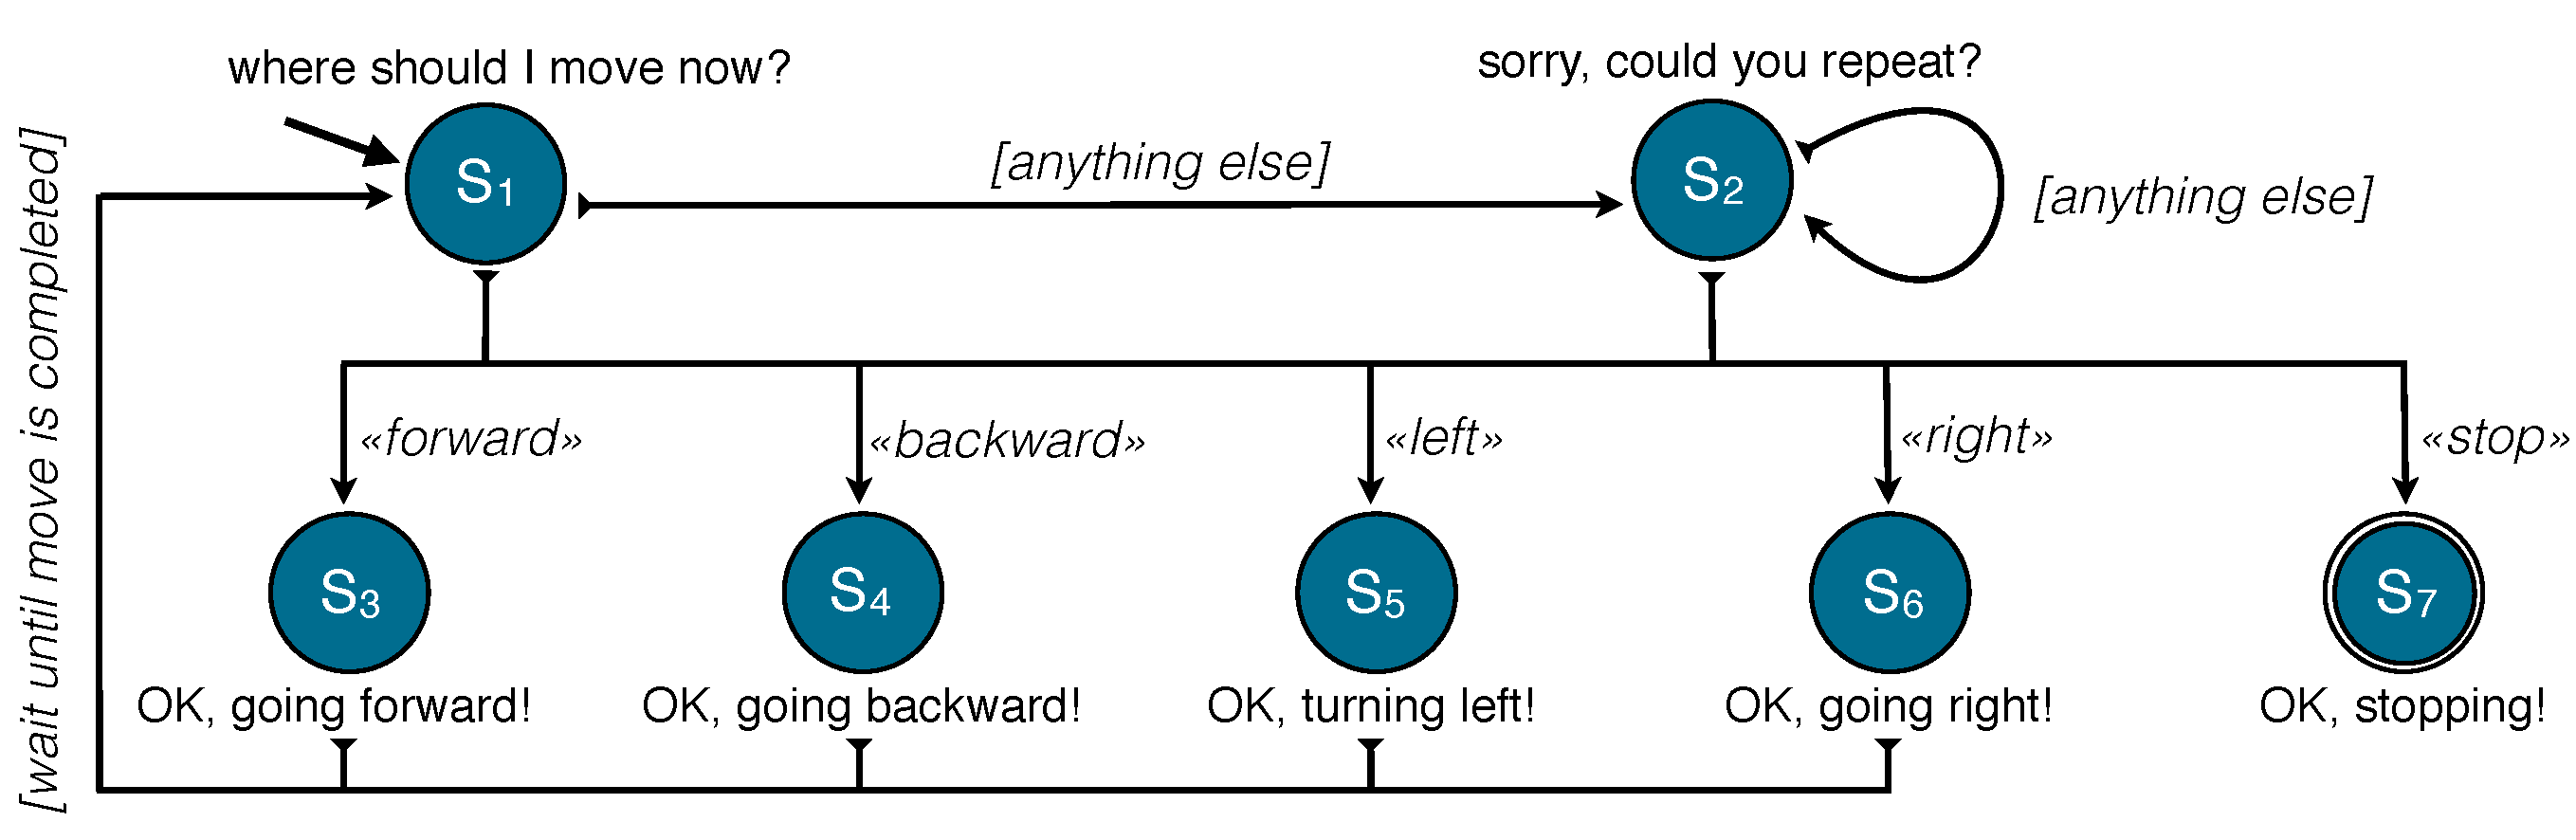
\includegraphics[scale=0.32]{imgs/fsa.pdf}
\caption{Example of finite-state automaton (FSA) for dialogue management, with seven possible states. The starting state for this FSA is $s_1$ and the (unique) ending state is $s_7$. The edges $s_3,... s_7 \rightarrow s_1$ are traversed once the movement is completed, and the two edges $s_1, s_2 \rightarrow s_2$ are traversed for any other user input than the five specified directions.}
\label{fig:fsa}
\end{figure}

A finite-state automaton is formally defined as a tuple $\langle \mathcal{S}, \Sigma, \delta, s_0, \mathcal{F} \rangle$, where $\mathcal{S}$ is the set of possible states, $\Sigma$ the set of inputs that the system can accept (in this case, the user dialogue acts, and possibly external events),  $\delta: \mathcal{S} \times \Sigma \rightarrow \mathcal{S}$ the transition function mapping every (state,input) pair to its successor state, $s_0$ the start state, and $\mathcal{F}$ the set of final states. 

Finite-state automata provide a simple and versatile framework for the development of a dialogue manager. Their expressive power is however rather limited, as the dialogue state of a FSA is represented as a single, atomic symbol, and the possible user moves by a finite enumeration of possible transitions allowed for each state.  Finite-state automata are therefore difficult to scale to more complex domains where the dialogue state might need to track multiple variables and allow for a large number of user dialogue acts.  

\subsubsection*{Logic- and plan-based approaches}

Richer representations of the dialogue state are required to overcome the rigidity of finite-state automata. A popular alternative builds on representations that encode the dialogue state as a frame constituted of a set of slot-value pairs \citep{seneff2000}.  Frame-based systems start with an empty frame that is gradually filled by the user inputs.  After each user move, a set of production rules define what actions to take  -- typically, a request to elicit a value for a particular slot -- based on the current frame.  The process continues until all slots are filled, which marks the completion of the dialogue. 

Due to their greater expressivity, frame-based systems offer a number of advantages in terms of domain modelling and dialogue control.  They remain however difficult to extend to other domains than classical slot-filling applications such as flight booking.  The \textit{information state} approach \citep{Larsson:2000} is an attempt to provide a more solid theoretical foundation for dialogue management in rich conversational domains.  As already mentioned in Section \ref{sec:architectures}, information state approaches rely on a blackboard architecture where various modules are attached to a central workspace called the information state. This information state is therefore continuously monitored by the modules integrated the dialogue system, and represent the full contextual knowledge available to the agent. In addition to the usual variables describing the dialogue history and the application task, the information state can also incorporate ``mentalistic'' entities such as the private and shared beliefs of the conversational agents.  The information state can exhibit a rich internal structure encoded as attribute-value matrices (AVMs) or typed records  \citep{RobinCooper2012}. 

Upon reception of a relevant input, the dialogue manager modifies this information state using a collection of update rules. In addition to state-internal operations that modify particular variables of the information state, the update rules are also employed to derive the actions to execute by the agent.  Given a collection of rules and a generic strategy to apply them, the dialogue manager can both update its state and select the next action to perform by way of logical inference. This action selection can notably be grounded on the set of open questions raised and not yet answered during the interaction \citep{larsson2002,Ginzburg2012}.  

Plan-based approaches such as the ones developed by \cite{Freedman:2000} and \cite{Allen:2001} take one step further. These approaches also rely on complex representations of the dialogue state that notably encompass the belief, desires and intentions (BDI) of each agent \citep{Cohen1979,Allen1980}.  But instead of update rules, classical planning is used to update the state and select the next action.  In such settings, both the user and the system are assumed to act in pursuit of their long term goals.  The interpretation of the user actions is thus cast as a \textit{plan recognition} problem, where the system seeks to derive the belief, desires and intentions that best explain the observed conversational behaviour of the speaker.  Similarly, the selection of system actions is derived from the (task-specific) long term objectives of the system. This search for the best action is an instance of a classical planning task, which can be solved using off-the-shelf planning algorithms. These algorithms require the declaration of a planning domain that specifies the preconditions and effects of every action. Agent-based frameworks such as the Constructive Dialogue Modelling approach developed by \cite{Jokinen:2009} follow similar principles, with a particular emphasis on conceptualising dialogue as a collaborative activity grounded in communicative principles of rational and coordinated interaction between agents. 

\subsubsection*{Benefits and limitations of hand-crafted approaches}

The primary benefits of hand-crafted approaches to dialogue management lie in their ability to capture rich conversational phenomena and endow the system designer with a fine-grained control over the application behaviour.  They have also laid the foundations for substantial advances in the semantic and pragmatic interpretation of dialogue moves \citep{ThomasonManuscript-THOEUA,Ginzburg2012}, the formalisation of social obligations \citep{Traum:1994}, the rhetorical structure of dialogue \citep{0521659515}, or the use of plan-based reasoning to infer the user intentions \citep{Allen1980,Litman87}.  They nevertheless suffer from two important shortcomings: \begin{enumerate}
\item They generally assume complete observability of the dialogue context and provide only a limited account (if any) of uncertainties. This assumption is unfortunately difficult to reconcile with the imperfections and restricted coverage of speech recognition and understanding.
\item They require the dialogue domain to be specified by hand, either through the definition of an finite-state automaton, a collection of update rules or a set of action schemas for planning.  This requirement is hard to satisfy for many domains, since the behaviour of real users is often challenging to anticipate (unsurprisingly, human behaviour can be difficult to predict) and can deviate significantly from the expectations of the system developers. 
\end{enumerate}

Statistical approaches, to which we now turn, have been specifically developed to address these two issues.

\subsection{Statistical approaches}
\label{sec:statistical}

Common to all statistical approaches to dialogue management is the idea of automatically optimising a dialogue policy (that is, a function associating each possible dialogue state to a system action) from interaction data.  Starting from this shared premise, statistical approaches vary along multiple dimensions such as the type of learning algorithm, the representation of the dialogue state and policy, and the nature of the data on which to estimate the models. We outline in this section the core concepts of statistical approaches, which will be exposed in a more formal setting in the next chapter. 

\subsubsection*{Supervised learning}

The first possible approach is to learn dialogue strategies by imitation based on examples of expert behaviour.  This expert behaviour can be recorded through so-called ``Wizard-of-Oz'' experiments.  As already mentioned in the introduction chapter, a Wizard-of-Oz experiment is an interaction in which a human user is asked to interact with a system that is remotely operated by a human agent (without the user being made aware of this control).  A hidden wizard is often preferred to a visible human interlocutor, as people tend to behave differently when they talk to a machine or a human person \citep{JonnsonD88}.  One can collect multiple interactions of this type and record the wizard decisions at each point, along with their context.   The resulting data set can be fed to a supervised learning algorithm in order to construct a dialogue policy that attempts to imitate the conversational behaviour of the wizard.  Learning the dialogue policy is thus seen as a classification problem with states as inputs and actions as outputs. The goal of the learning algorithm is then to construct a classifier  that optimises the classification accuracy for the Wizard-of-Oz data set, considering the wizard actions as ``gold standards''.  This classifier can be estimated with any standard machine learning methods (decision trees, logistic regression, etc.).
 
In a supervised setting, action selection is essentially viewed as a sequence of isolated decision problems.  As argued by \cite{817450}, this formalisation ignores some important characteristics of conversational behaviour. Dialogue is fundamentally a dynamic process where the state and action at time $t$ have a direct influence on the resulting state at time $t+1$.  This temporal connection between states is typically lost with classical supervised learning approaches. Furthermore, the state space grows exponentially with the number of state variables, and can therefore reach very large sizes.  The training data available from a fixed Wizard-of-Oz corpus will therefore only cover a fraction of the state space for the domain.  As a consequence, many states encountered at runtime will have no appropriate training examples on which to ground the action selection.  Generalisation techniques can however be used to mitigate this problem of data sparsity. 

% note about our approach: generalisation enable a better account of the data sparsity problem.  plus, the state dynamics are not lost since we perform belief update.  Finally, the appraoch can be seen as an initial boostrapping that can then be further refined through online reinforcement learning (Bayesian prior), as in Williams etc. also, we learn utilities, not a direct classification. Also: a user simulator is difficulty for situated and open-ended environments.  we learn a POMDP policy by simulation

\subsubsection*{Reinforcement learning}

Reinforcement learning (RL) presents an attractive solution to the problem of dialogue policy optimisation.  A reinforcement learning problem typically revolves around an \textit{agent} interacting with its environment, typically to perform some practical task.  Through its actions, the agent is able to change the state of its environment.  After each action, the agent can observe both the new environment state resulting from its actions, as well as a numerical reward encoding the immediate value (positive or negative) of the executed action in relation to the agent's goal. The goal of the learning agent is to find the best action to execute in any given state via a process of trial and error  -- the best action being characterised as the one that maximise the agent's expected long-term reward.  

Reinforcement learning tasks are generally formalised using \textit{Markov Decision Processes} (MDPs), which are defined as tuples $\langle \mathcal{S}, \mathcal{A}, T, R \rangle$ with a state space $\mathcal{S}$, an action space $\mathcal{A}$, a transition function $T$ that encodes  the probability $P(s'|s,a)$ of reaching state $s'$ after executing action $a$ in state $s$, and a reward function $R$ that specifies the reward value associated with the execution of action $a$ in state $s$. Dialogue can be expressed as a Markov Decision Process where the state space corresponds to the possible dialogue states and the actions to the set of (verbal or extra-verbal) actions available to the dialogue agent.  The transition function $T$ captures the ``dynamics'' of the conversation, and indicates how the dialogue state is expected to change as a result of the system actions. Finally, the reward function $R$ expresses the objectives and costs of the application. A common reward function is to assign a high positive value for the successful completion of the task, a high negative value for a failure, and a small negative value for soliciting the user to repeat or clarify her/his intention.  

Given a particular MDP problem, the goal of the learning agent is to find a policy $\pi: \mathcal{S} \rightarrow \mathcal{A}$ that maps each possible state to the best action to execute at that state.  The best action is defined as the action that maximises the \textit{expected return} for the agent.  Simply put, the return is the long-term (discounted) accumulation of rewards from the current state up to a given horizon. 

Various learning methods have been devised to automatically extract this optimal policy from interaction experience. Due to the large amounts of cycles that are necessary to converge onto an optimal policy, direct interactions with real users are often impossible or highly impractical for many domains. Instead, most recent approaches have relied on the construction of a user simulator able to generate unlimited numbers of interactions on the basis of which the dialogue system can optimise its policy.  
The user simulator can either be designed by experts  or ``bootstrapped'' from existing datasets  or Wizard-of-Oz studies \citep{InTech_RL_2008_OP,FramptonL09}. The reliance on a user simulator for policy optimisation has the major advantage of allowing the learning agent to explore millions of dialogue trajectories on a scale that would be impossible to achieve with real users.  Simulated interactions run however the risk of deviating from real user behaviours.

A limitation faced by MDP approaches is the assumption that the dialogue state is fully observable. As frequently noted in the course of this thesis, this assumption simply does not hold for most dialogue domains, owing to the presence of multiple sources of uncertainty, in particular speech recognition errors.  An elegant solution to this problem is to extend the MDP framework by allowing the state to be a hidden variable that is indirectly inferred from observations.  Such extension gives rise to a  \textit{Partially Observable Markov Decision Process} (POMDP).  POMDPs are formally defined as tuples $\langle \mathcal{S}, \mathcal{A}, T, R, \mathcal{O}, Z \rangle$.  As in a classical MDP, $\mathcal{S}$ represents the state space, $\mathcal{A}$ the action space, $T$ the transition probability $P(s'|s,a)$ between states, and $R$ the reward function $R(s,a)$.  However, the actual state is no longer directly observable.  Instead, the process is associated with an observation space $\mathcal{O}$ that expresses the set of possible observations that can be perceived by the system (for instance, the N-best lists of user dialogue acts generated by the speech recogniser and NLU modules) . The function $Z$ finally defines the probability $P(o|s)$ of observing $o$ in the current state $s$.  

In the POMDP setting, the agent knowledge at a given time is represented by the \textit{belief state} $b$, which is a probability distribution $P(s)$ over possible states.  The belief state is continuously updated as additional information becomes available in the form of e.g. new observations. Based on this belief state, a POMDP policy is defined as a function mapping each possible belief state to its optimal action.  As for MDP-based reinforcement learning, POMDP approaches usually derive the dialogue policy from interactions with a user simulator  \citep{Young:2010,Thomson:2010:BUD:1772996.1773040, daubigney2012}. The optimisation process is however considerably more complex than for MDPs, as the belief state is a continuous and high-dimensional structure. Approximation techniques are therefore necessary in order to extract dialogue policies of reasonable quality in such complex space. The next chapter fleshes out the theoretical foundations of these modelling strategies and their applications to spoken dialogue systems.

\subsubsection*{Benefits and limitations of statistical approaches}

%To conclude this section on statistical approaches to dialogue management, it is useful to recapitulate the major benefits and limitations of statistical approaches compared to the more traditional hand-crafted strategies.  

As stated in the previous sections, one key benefit of statistical approaches is the improved robustness towards errors and unexpected events. This robustness stems primarily from the use of probabilistic reasoning techniques that explicitly account for the uncertainty inherent in spoken dialogue.  The second benefit is the possibility to optimise dialogue policies in a principled, data-driven manner based on a generic specification of the system objectives expressed in the reward function.  This specification allows the system designer to explicitly encode the various goals and costs of the system. This ability to represent trade-offs between multiple, sometimes conflicting objectives is one important advantage of reinforcement learning approaches.  Empirical studies have shown that automatically optimised policies can outperform hand-crafted strategies in both simulated environments and  real user trials, based on objectives and subjective metrics of dialogue success \citep{Supelec270,6407655}. 

Statistical modelling techniques come however with a number of challenges of their own. The most pressing issue is the paucity of suitable data sets.  Statistical models often require large amounts of training data to estimate their parameters. Unfortunately, real interaction data is scarce, expensive to acquire, and difficult to transfer from one domain to another.  User simulators can partly alleviate this problem, but must often themselves be bootstrapped from data, and offer no guarantee of producing conversational behaviours that reflect those of real users.  The computational complexity of the learning algorithm can also be problematic. Statistical approaches -- and especially POMDP-based systems -- must often carefully engineer their state and action variables to limit the size of the search space and ensure the learning process remains tractable.  Albeit several dimensionality reduction techniques have been proposed in the literature \citep{williams2005,Young:2010,Cuayahuitl:2010,CrookL11}, most work has so far concentrated on slot-filling applications.   Domains such as tutoring systems, cognitive assistants and human-robot interaction must however often deal with state-action spaces that are considerably more elaborate, with multiple tasks to perform, sophisticated user models, and a complex, dynamic environment.  In such settings, the dialogue system might need to track a large number of variables in the course of the interaction, which quickly leads to a combinatorial explosion of the state space.  How to define appropriate statistical models for these open-ended dialogue domains remains an open question, to which the present thesis aims to offer preliminary answers. 

Finally, many practical dialogue applications need to enforce generic constraints on the dialogue flow.  Such constraints may for instance correspond to business rules specific to the particular application.  The incorporation of such constraints in the optimisation process of dialogue policies is however far from trivial. As noted by \cite{Paek:2008}, this lack of direct control on the final policy is one of the main reasons for the slow adoption of RL approaches in industrial systems.  Although some researchers have worked on the integration of expert knowledge into dialogue policy learning \citep{williams2008,Henderson:2008}, much work remains to be done to bring about a unified approach to dialogue management that combines the robustness of data-driven approaches with the control and expressivity of hand-crafted strategies. 

Table \ref{table:approaches} presents a comparison of the most important hand-crafted and statistical methods to dialogue management in terms of state representation, account of state uncertainty (in the sense of having multiple hypotheses about the current state, each one assigned with a specific probability), type of state update and action selection mechanism.  The last row also describes how the approach developed in this thesis stands in comparison to these methods. 
  
\renewcommand{\arraystretch}{2.0}
\setlength{\tabcolsep}{8pt}
\begin{sidewaystable}
\begin{center}
\begin{tabular}{|p{55mm}||p{31mm}|p{16mm}|p{50mm}|p{66mm}|} \hline
\centering \textbf{Approach} &  \centering \textbf{State representation} &  \centering \textbf{State uncertainty} &  \centering \textbf{State update mechanism} & \textbf{Action selection mechanism} \vspace{5pt} \\  \hline \hline
Finite state automata & Atomic state & no & Traversal of matching edge & Action associated with node \vspace{5pt} \\ \hline
Frame-based systems \; \; \; \; \; \; \; \; \; \; \; \; \begin{footnotesize}\citep[e.g.][]{seneff2000}\end{footnotesize}& Slot/value pairs & no & Slot-filling given user inputs & Production rules \vspace{5pt} \\ \hline
Information state update \; \; \; \; \; \; \begin{footnotesize}\citep[e.g.][]{Larsson:2000}\end{footnotesize} & Rich typed feature structure \vspace{5pt} & no & Update rules & Decision rules \vspace{5pt} \\ \hline
Plan-based systems   \; \;  \; \; \; \; \; \; \; \; \begin{footnotesize}\citep[e.g.][]{Freedman:2000,Allen:2001}\end{footnotesize} & BDI model \vspace{5pt} & no & Plan recognition and update of BDI model & Classical planning \vspace{5pt} \\ \hline
Supervised approaches \; \; \; \; \; \; \; \; \begin{footnotesize}\citep[e.g.][]{Hurtado:2005}\end{footnotesize} & Atomic/factored state & no & Extraction of state variables from history and task status & Classifier estimated from Wizard-of-Oz data by supervised learning\vspace{5pt} \\ \hline
MDP-based systems  \; \; \; \; \; \; \; \; \begin{footnotesize}\citep[e.g.][]{Walker:2000,817450}\end{footnotesize} & Atomic/factored state & no & Extraction of state variables from history and task status & Policy optimised via reinforcement learning from real or simulated dialogues \vspace{5pt} \\ \hline
POMDP-based systems \; \; \; \; \; \; \begin{footnotesize}\citep[e.g.][]{Roy:2000,Young:2010}\end{footnotesize}\vspace{5pt} & Atomic/factored state & yes & Update of belief state & Policy optimised via reinforcement learning from real or simulated dialogues \vspace{5pt} \\ \hline
Probabilistic rules & Factored state & yes & Structured belief state update (with probabilistic rules) & Policy optimised via (Bayesian) supervised or reinforcement learning \vspace{5pt} \\ \hline 
\end{tabular}
\end{center}
\caption{Comparison of dialogue management approaches.}
\label{table:approaches}
\end{sidewaystable}


\section{Summary}

We have presented in this chapter the most important concepts and methods in the area of dialogue processing and management.  Starting with a linguistic analysis of the most important dialogue phenomena, we discussed several key aspects of verbal interactions, such as their articulation in sequences of turns and dialogue acts. We also stressed the importance of contextual knowledge in the interpretation and production of dialogue acts, and the role of grounding signals to maintain mutual understanding among the conversational partners. 

Section \ref{sec:sds} described how spoken dialogue systems are internally structured. As we have explained, dialogue systems are often instantiated in complex software architectures that comprise numerous interconnected components for tasks such as speech recognition, understanding, dialogue management, natural language generation and speech synthesis.  Dialogue systems can also be extended to handle (i.e. both perceive and act upon) extra-linguistic modalities and environmental factors. The range of possible applications of dialogue system technology is broad and includes domains as varied as mobile applications for information access and service delivery, in-car navigation systems, smart home environments, cognitive assistants, tutoring systems, and service robots. 

The last section presented an overview of the dialogue management task. A key concept shared by virtually all approaches to dialogue management is the \textit{dialogue state}, a data structure used to encode the system knowledge of the current conversational situation.  This dialogue state can take multiple forms, from the atomic symbols used in finite-state approaches to the rich nested feature structures employed in information state formalisms. Based on this dialogue state, an action selection mechanism is then responsible for the selection of the next action to execute.  In hand-crafted approaches, this mechanism is manually specified by the application developer, either via direct mappings from state to actions, or indirectly through the use of planning techniques.  Statistical approaches, on the other hand, seek to automatically optimise dialogue policies from (real or simulated) interaction data.  A wide range of learning techniques have been developed to perform this optimisation, from supervised learning on a Wizard-of-Oz data set to reinforcement learning based on a user simulator and a generic reward function.   Reinforcement learning techniques can themselves be divided into MDP approaches, where action effects are stochastic but the dialogue state itself is assumed to be known, and POMDP approaches, which incorporate both stochastic action effects and state uncertainty.

We concluded our review of dialogue management approaches by noting that both hand-crafted and statistical methods have significant challenges to address.  This is especially striking for open-ended domains such as human-robot interaction, which exhibit both high levels of noise and uncertainty and a rich dialogue context.   One of the central claims of this thesis is that these domains are best addressed with a hybrid approach to dialogue management that combines probabilistic modelling with expert knowledge about the domain structure.  Chapter \ref{chap:rules} presents how such modelling approach can be formalised.  But before doing so, we first need to lay down the mathematical apparatus required for designing probabilistic models of dialogue, which is the subject of the next chapter.



\chapter{Probabilistic rules}
\label{chap:rules}

The previous chapter fleshed out how dialogue could be represented as a stochastic process and described the benefits of using graphical models to efficiently encode the probability and utility models employed in dialogue management. Plain graphical models must however face non-trivial scalability issues when applied to dialogue domains associated with rich conversational contexts. The number of parameters necessary for state update and action selection can indeed increase rapidly with the complexity of the domain models. Alas, only small quantities of genuine training data are available in most dialogue domains, and usually cover only a small fraction of the state-action space of interest. 

To address this discrepancy between the size of the parameter space and the amount of data available to estimate them, we introduce in this chapter a new approach to probabilistic dialogue modelling, based on the notion of \textit{probabilistic rules}.  Probabilistic rules are structured mappings between conditions and effects, and function as \textit{high-level templates} for the construction of a dynamic decision network.  The key advantage of this structured modelling approach is the drastic reduction of the number of parameters compared to traditional representations.  We also argue that these expressive representations are particularly well suited to encode the probability and utility models of dialogue domains, where substantial amounts of expert knowledge can often be leveraged to structure the relationships between variables. 

The chapter is divided in six sections. Section \ref{sec:rmotivation} exposes in general terms how structural assumptions can be applied to reduce the size and complexity of probabilistic models.  Section \ref{sec:formalisation} defines the formalism of probabilistic rules and its main theoretical properties.  These definitions are then connected in Section \ref{sec:ruleinstantiation} to the graphical models described in the previous chapter by showing how the rules are practically instantiated in the Bayesian network representing the dialogue state. Section \ref{sec:processing-workflow} explains how this instantiation procedure is incorporated in the processing workflow for updating the dialogue state and selecting the system actions. Finally, Section \ref{sec:amodelling} addresses some advanced modelling questions and Section \ref{sec:relatedwork} relates the approach to previous work.


\section{Structural leverage}
\label{sec:rmotivation}

The starting point of our approach is the observation that the probability and utility models used in dialogue management often exhibit a fair amount of \textit{internal structure}.  
We have already discussed in the previous chapter one simple instance of this internal structure, namely factored representations based on conditional independences. However, the internal structure of dialogue domains does not limit itself to these basic independence assumptions, and much can be gained by exploiting other types of structural properties, as shall be argued in the next pages. 

%If two sets of random variables $\mathbf{X}$ and $\mathbf{Y}$ are conditionally independent given $\mathbf{Z}$, we can rewrite the probability distribution $P(\mathbf{X}, \mathbf{Y} \, | \, \mathbf{Z})$ as $P(\mathbf{X} \, | \, \mathbf{Z}) (\mathbf{Y} \, | \, \mathbf{Z}) $.  


\subsubsection*{Latent variables}
 
The number of parameters required to estimate the distributions of a graphical model can often be reduced by introducing \textit{latent variables} (i.e. unobserved or hidden variables) that act as intermediaries between the source and target variables. Indeed, many application domains are often best explained by the combination of a small number of distinct factors or influences, each encoded by a separate random variable and associated with a subset of input and output variables. This layer of latent variables is usually never observed directly but contribute to structuring the model.\footnote{The construction of layered computational models is one of the most active research topic in artificial intelligence and machine learning, and form in particular the foundations of deep learning approaches \citep{Bengio:2009}.} In the particular case of medical diagnosis, the relations between predisposing factors and observed symptoms are for instance best described by postulating an intermediary layer of variables -- possible diseases -- that mediates between the predisposing factors and the observed symptoms.  Figure \ref{fig:latentvariables} illustrates how latent variables can be exploited to provide an additional layer of abstraction within a graphical model.

 \begin{figure}[h]
\centering
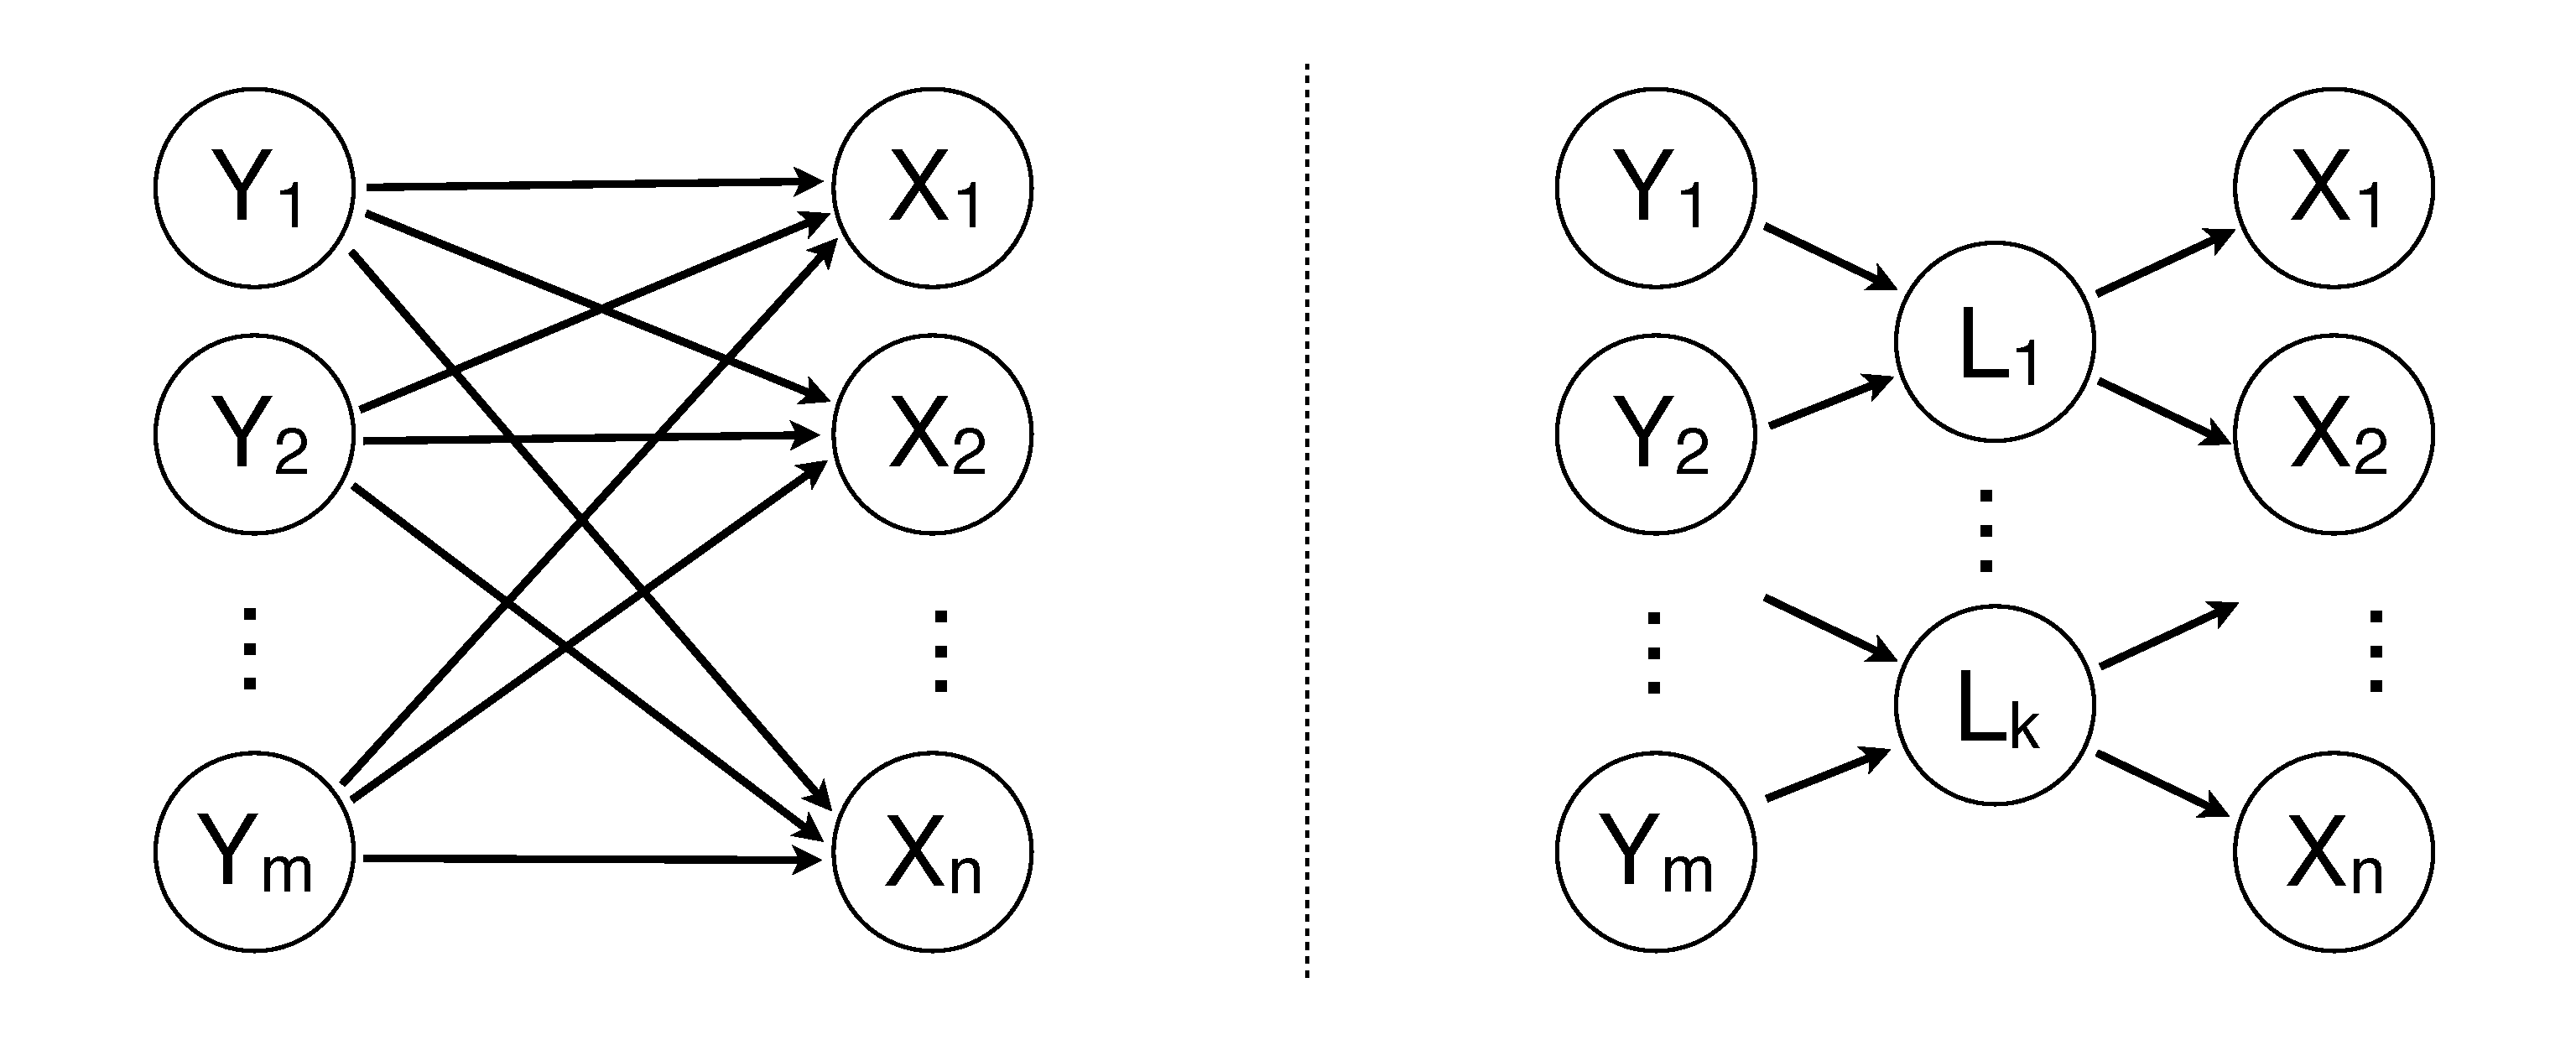
\includegraphics[scale=0.25]{imgs/latentvariables.pdf}
\caption{Comparison between a model that directly maps variables $\mathbf{Y}$ to $\mathbf{X}$ (left side) and one relying on latent variables $\mathbf{L}$ to serve as intermediaries (right side).}
\label{fig:latentvariables}
\end{figure}

Dialogue models can benefit from the inclusion of such latent variables. The transition function can for instance be modelled in terms of a limited number of latent variables, each responsible for capturing specific aspects of the interaction dynamics.  We shall see in the forthcoming sections that probabilistic rules precisely operate as latent variables when instantiated in the dialogue state. 

\subsubsection*{Partitioning}

A random variable $X$ with parent variables $Y_1,...Y_m$ must specify a separate probability distribution for every possible assignment of values for the parent variables. In other words, the number of parameters required to specify the distribution $P(X \, | \, Y_1,..., Y_m)$ is exponential in the number of parents $m$. Fortunately, the values of these parents variables can be grouped into \textit{partitions} yielding similar outcomes for $X$. One can therefore directly define the conditional probability distributions on these groups rather than on the full enumeration of combined values for the parent variables. Partitioning is an example of \textit{abstraction mechanism} which can be used to reduce the model complexity and improve its ability to generalise to unseen examples. 

%Utility distributions can also partition the values of their dependent variables in a similar way.  

Figure \ref{fig:partitioning} illustrates such partitioning operation for the conditional probability distribution $P(\mathit{Fire} \, | \mathit{Weather}, \mathit{Rain})$.  The space of possible values for the parent variables is defined in this example as $Val(\mathit{Weather}) \times Val(\mathit{Rain})$ and contains 6 possible elements.  We can observe that this space can be split in two partitions: $\mathit{Rain}\!=\mathit{true} \lor \mathit{Weather}\!\neq\mathit{hot}$ and $\mathit{Rain}\!=\mathit{false} \land \mathit{Weather}\!=\mathit{hot}$. This partitioning allows a significant reduction of the number of parameters required for the conditional probability distribution.  It should be noted that grouping value assignments into partitions corresponds to a modelling choice and can degrade the model accuracy if the partitions do not reflect actual similarities in the predicted outcomes.

%As illustration, consider a minimalistic dialogue in a robot learning scenario where the robot can ask the user yes/no questions pertaining to the colour of one specific object (e.g. \utt{Is the object red?}). In this simple scenario, the state is represented with two variables: the user dialogue act $a_u = \{\mathit{yes,no}\}$ and a variable representing the object colour, $\mathit{colour} = \{\mathit{blue,green, ...}\}$ with $n$ possible colours.  The system actions take the form $a_m = \{ \mathit{VerifyColour(c)}: c \in \mathit{colour}\}$, where $VerifyColour(c)$ corresponds to asking the user whether the object is of colour $c$.  Since the object colour remains constant, the transition function for this domain is defined as $P(a_u'|a_m, \mathit{colour})$. The number of parameters required to specify the transition function is $n^2$ (since $a_m$ and $\mathit{colour}$ have $n$ possible values each). 

%However, one can reasonably assume in this example that the particular colour mentioned in the question is irrelevant to predict the next user dialogue act $P(a_u'|a_m,\mathit{colour})$ as long as it matches (or fails to match) the actual colour of the object.  Based on this assumption, one can divide the space $Val(a_m) \times Val(\mathit{colour})$ into two distinct partitions: 
%\begin{enumerate}
%\item One partition in which the verification question corresponds to the actual colour of the object: $\exists c: colour\!=\!c \land a_m\!=\!\mathit{VerifyColour(c)}$.
%\item One partition in which there is a mismatch between the colour mentioned in the question and the actual colour: $\exists c: colour\!=\!c \land a_m\!\neq\!\mathit{VerifyColour(c)}$.
%\end{enumerate}

%By abstracting over the specific colour mentioned in the question, partitioning allows us to drastically reduce the number of parameters required for the conditional probability distribution $P(a_u'|a_m,\mathit{colour})$ from a total of $n^2$ to only $2$. Figure \ref{fig:partitioning} illustrates this reduction. 


 \begin{figure}[h]
\centering
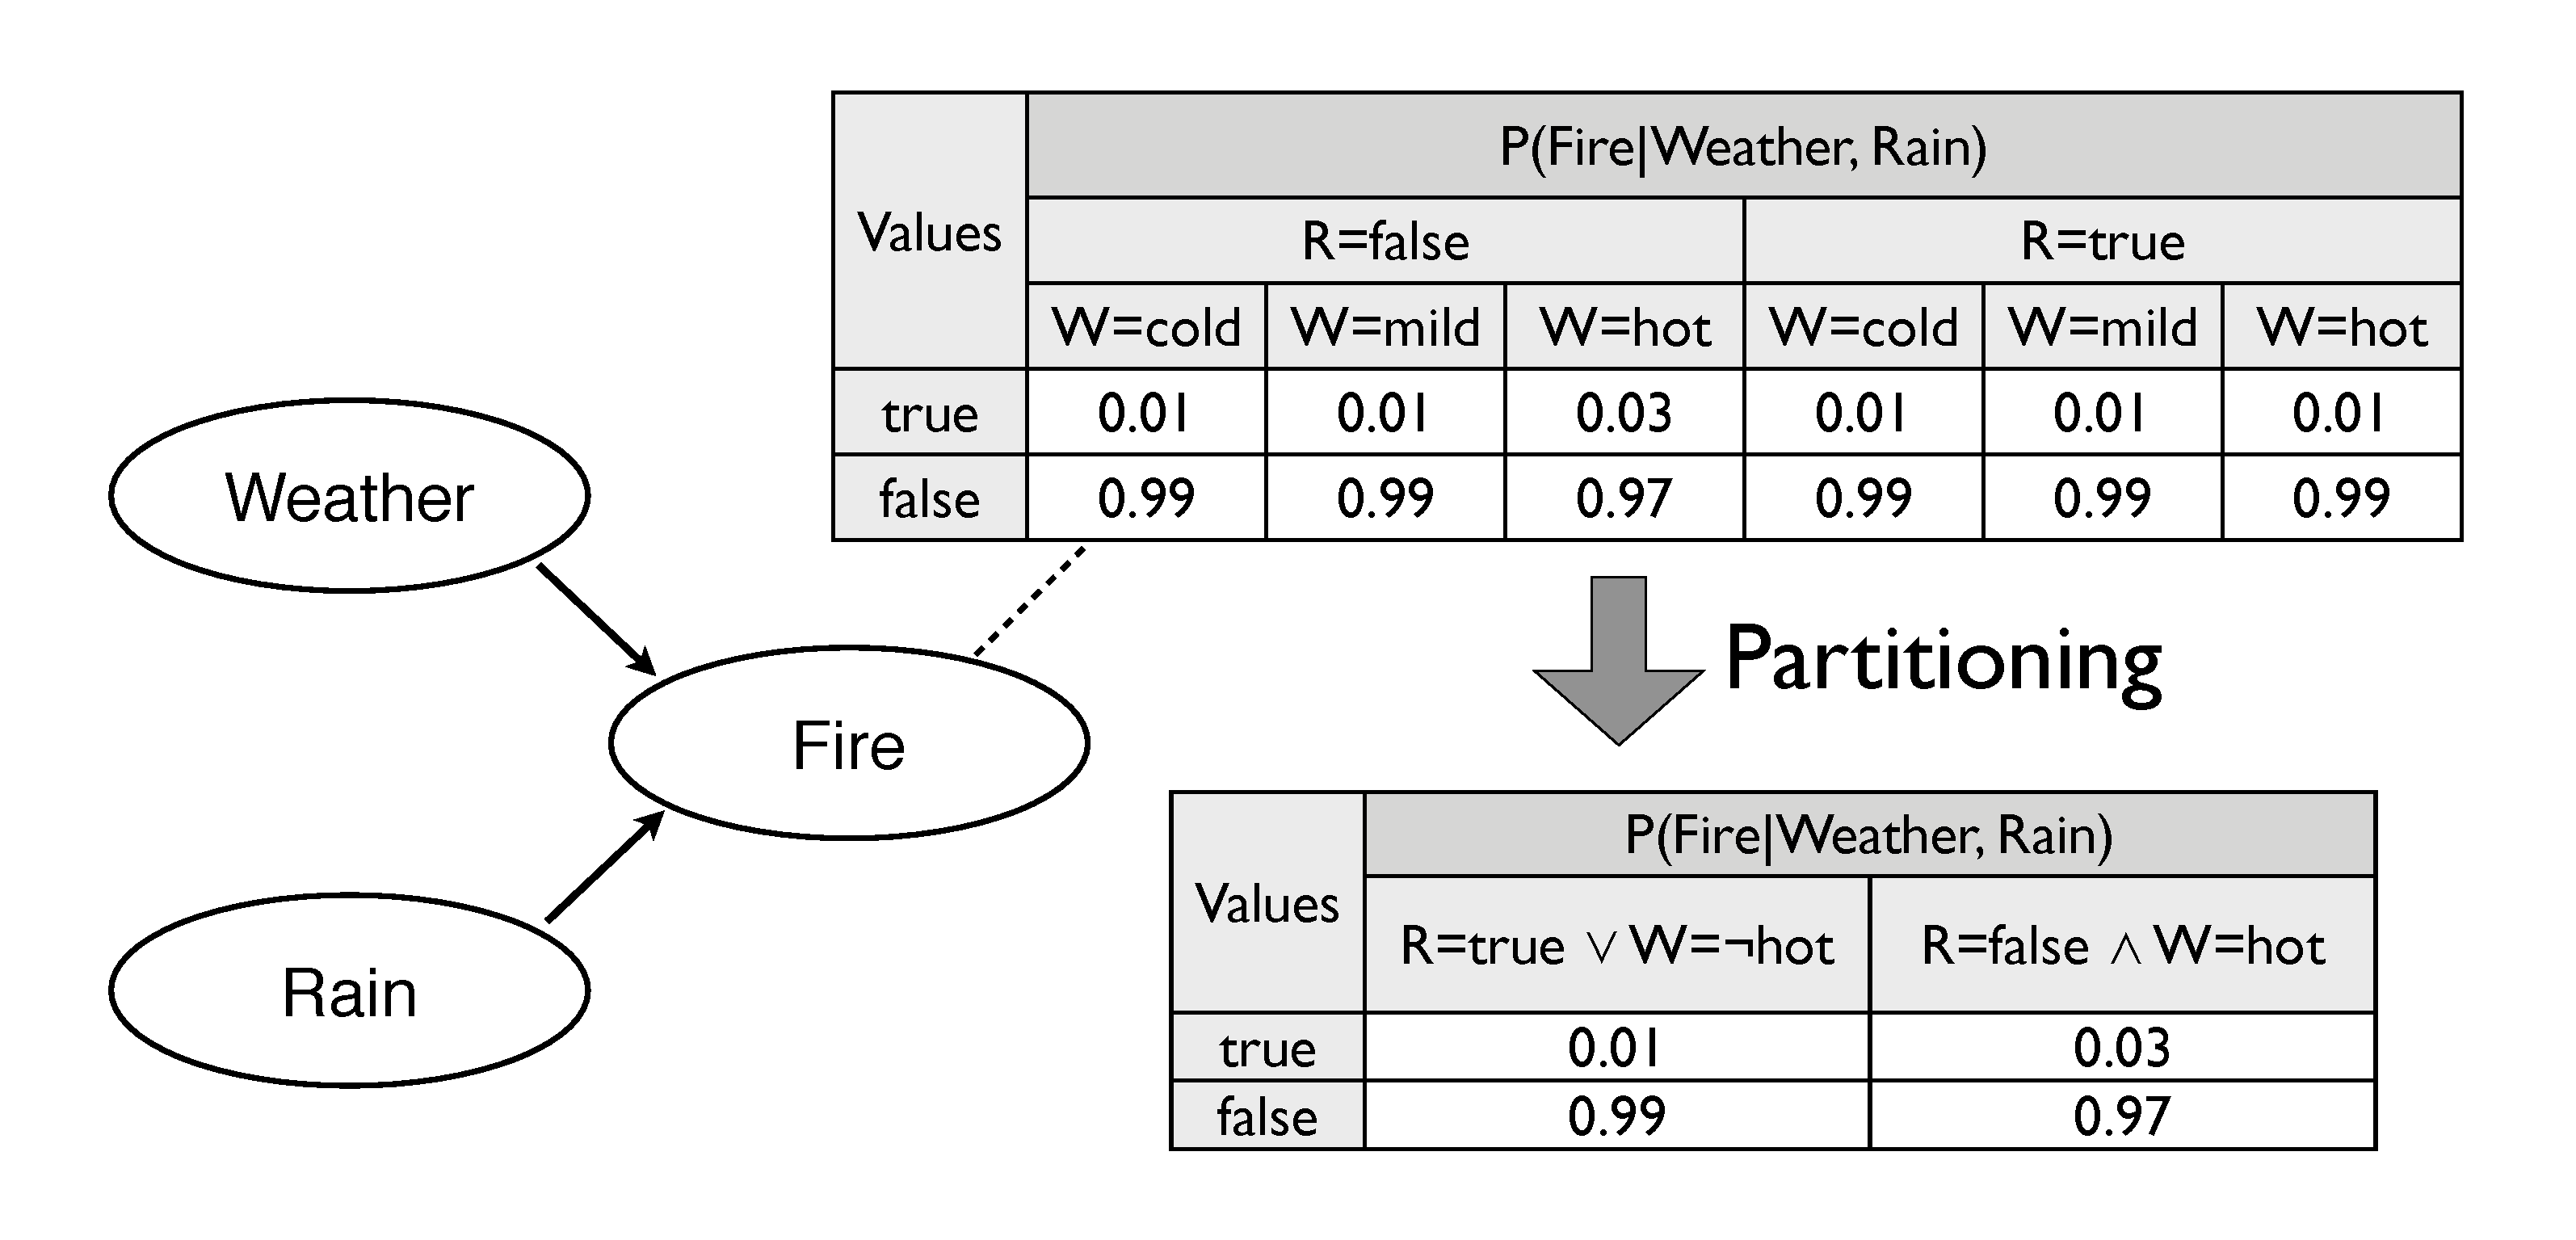
\includegraphics[scale=0.25]{imgs/partitioning.pdf}
\caption{Partitioning for the conditional probability distribution $P(\mathit{Fire} \, | \mathit{Weather}, \mathit{Rain})$.}
\label{fig:partitioning}
\end{figure}

Partitions must be both exhaustive (each combination of values for the parent variables must belong to one partition) and mutually exclusive (a combination of values can only belong to one partition).  As we can observe from the example, partitions can often be concisely expressed via logical conditions on the variable values.  A given assignment of values is then grouped in a partition if it satisfies the condition associated with it.

\subsubsection*{Quantification}

Many dialogue domains are composed of objects or entities related to one another. These domains are often difficult to directly encode by a fixed set of random variables, as the number of entities and relations may vary over time.  Examples of relational structures include: 
\begin{itemize}
\item Collections of physical objects in a visual scene, each described by specific features (colour, shape) and relations with other objects (e.g. spatial relations),
\item Indoor environments topologically structured in rooms and spaces in which to navigate. 
\item Stacks of tasks to complete by the agent, each task being possibly connected to other tasks via precedence or inclusion relationships.
\item Linguistic entities employed in the dialogue acts of the conversational partners, linked with one another through multiple syntactic, semantic, referential or pragmatic relations. 
\end{itemize}

First-order logic provides an excellent basis for representing and manipulating such relational structures, as it offers a principled language for (1) referring to objects connected with one another through functions and relations and (2) describing their properties in a concise way through the use of universal and existential quantifiers.\footnote{We shall not cover in this thesis the mathematical foundations of first-order logic, but the interested reader is invited to refer to e.g. \cite{gamut1991logic} for a formal overview of the logical concepts mentioned throughout this thesis.}

Graphical models represent relational domains by instantiating one random variable for every possible grounding of the functions and predicates defined for the domain for a collection of objects.\footnote{Such operation is akin to \textit{propositionalisation} in the terminology of first-order logic.}  A domain with two objects $o_1$ and $o_2$ and a relation $\mathit{leftOf}(x,y)$ will for instance generate the four groundings $\mathit{leftOf}(o_1,o_2)$, $\mathit{leftOf}(o_2,o_1)$ $\mathit{leftOf}(o_1,o_1)$ and $\mathit{leftOf}(o_2,o_2)$. The definition of probability and utility distributions that can handle the relational semantics of such representation is however problematic. In particular, generic properties and constraints such as $\forall x, \neg \mathit{leftOf}(x,x)$ and $\forall x, y, z, \mathit{leftOf}(x,y) \land \mathit{leftOf}(y,z) \Rightarrow \mathit{leftOf}(x,z)$ can be difficult to enforce at a global level, since classical probabilistic models offer no direct support for quantifiers.  Their expressive power is indeed intrinsically limited to propositional logic. 
 
The unification of first-order logic and probability theory has spanned a new research area called \textit{statistical relational learning} \citep{getoor:srlbook07}. A common trait of most approaches to statistical relational learning is the definition of a logic-based description language which is employed as a template to generate classical probabilistic models given a set of constants. The introduction of quantifiers provide an abstraction mechanism to reduce the complexity of probability and utility models by describing constraints or relations that hold for all possible groundings of a given formula and can therefore apply to large sets of random variables. 

\section{Formalisation}
\label{sec:formalisation}

We now outline a generic description framework for expressing the various types of internal structure we have just detailed.  This description framework revolves around the notion of \textit{probabilistic rules}.The framework was originally presented in \cite{rulebasedmodels-sigdial2012,lison-semdial2012}.

The key idea is to represent distributions with the help of \textit{if ... then ... else} control structures, based on the following skeleton:
\begin{equation*}
\begin{aligned}
& \textbf{if} \ \ (\text{condition 1 holds}) \ \ \textbf{then} \\ 
& \;\;\;\;\; \text{Distribution 1 over possible effects} \\
& \textbf{else if} \ \ (\text{condition 2 holds}) \ \ \textbf{then} \\ 
& \;\;\;\;\; \text{Distribution 2 over possible effects} \\
& ... \\
& \textbf{else} \\
& \;\;\;\;\; \text{Distribution } n \text{ over possible effects} \\ 
\end{aligned}
\label{eq:probrule}
\end{equation*}

Each \textit{if ... then} branch specifies both a \textit{condition} on particular state variables and an associated distribution over possible \textit{effects}.   The \textit{if ... then ... else} structure is read in sequential order, as in programming languages, until a satisfied condition is found, which causes the activation of the corresponding probabilistic effects. 

We first present how probabilistic rules can express conditional probability distributions in terms of structured mappings between input and output variables.  We then show how to  generalise the formalism to utility distributions and extend it with quantification mechanisms.

A terminological note is here in order: we shall use the term \textit{probabilistic rules} as an umbrella term that covers all types of rules in this thesis, while \textit{probability rules} will only refer to rules expressing probability distributions over effects, and \textit{utility rules} to rules expressing utility distributions.

\subsection{Probability rules}
\label{sec:probabirules}

Probability rules take the form of \textit{if ... then ... else} control structures and map a list of conditions on input variables to probabilistic effects on output variables. More formally, a rule is expressed as an ordered list $\langle br_1, ... br_{n}\rangle$, where each branch $br_i$ is a pair $(c_i, P(E_i))$, $c_i$ is a condition and $P(E_i)$ an associated distribution over possible effects.  The distribution $P(E_i)$ is a categorical distribution with possible effects $Val(E_i) = \{e_{(i,1)},... e_{(i,m_i)}\}$, where $m_i$ is the number of alternative effects in $P(E_i)$.  Each effect $e_{(i,j)} \in Val(E_i)$ has a particular probability denoted $p_{(i,j)}$. 

Given these elements, a basic probability rule reads as such:
\begin{equation}
\begin{aligned}
& \textbf{if} \ \ (c_{1}) \ \ \textbf{then} \\ 
& \;\;\;\;\; \begin{cases}
P(E_1\!=\!e_{(1,1)}) = p_{(1,1)} \\
 ... \\
P(E_1\!=\!e_{(1,m_1)}) = p_{(1,m_1)} 
\end{cases} \\[3mm]
& \textbf{else if} \ \ (c_{2}) \ \ \textbf{then} \\ 
& \;\;\;\;\; \begin{cases}
P(E_2\!=\!e_{(2,1)}) = p_{(2,1)} \\
 ... \\
P(E_2\!=\!e_{(2,m_2)}) = p_{(2,m_2)}
\end{cases} \\ 
& ...  \\
& \textbf{else} \\
& \;\;\;\;\; \begin{cases}
P(E_{n}\!=\!e_{(n,1)}) = p_{(n,1)} \\
... \\
P(E_{n}\!=\!e_{(n,m_n)}) = p_{(n,m_n)}
\end{cases}
\end{aligned}
\label{eq:probrule}
\end{equation}

 In the rest of this thesis, we will often use $P(e_{(i,j)})$ as notational convenience for $P(E_i = e_{(i,j)})$.   

%The three following sections describe how the conditions $c_i$, effects $e_{(i,j)}$ and associated effect probabilities $p_{(i,j)}$ are respectively defined. 

\subsubsection*{Conditions}

The conditions $c_i$ are expressed as logical formulae grounded in a subset of random variables defined in the dialogue state. This subset of state variables are the \textit{input variables} of the rule, which we shall denote as $I_1,...I_{k}$. Conditions can be arbitrarily complex logical formulae connected by conjunction, disjunction and negation, and (as we shall see in Section \ref{sec:quantification}) can also include universally quantified variables. The examples $(\mathit{Rain}\!=\mathit{true} \lor \mathit{Weather}\!\neq\mathit{hot})$ and $(\mathit{Rain}\!=\mathit{false} \land \mathit{Weather}\!=\mathit{hot})$ in Figure \ref{fig:partitioning} are instances of valid conditions on the two input variables $Rain$ and $\mathit{Weather}$. 

Given that a rule is defined through a \textit{if ... then ... else} control structure, the partitioning is guaranteed by construction to be exhaustive and mutually exclusive (only one branch will be followed).  When provided with an assignment of values on the input variables, the conditions are tested in sequential order until one is satisfied. When no terminating \textbf{else} block is explicitly specified at the end of a rule, the framework assumes a final \textbf{else} block associated with a void effect to ensure that the partitioning is exhaustive. The last condition $c_n$ is thus guaranteed to be always trivially satisfied irrespective of the input variable values. 

The conditions on the input variables offer a compact partitioning of the state space to mitigate the dimensionality curse.  Without this partitioning in alternative conditions, a rule ranging over input variables $I_1,...I_{k}$ each containing $q$ possible values would need to enumerate $q^{k}$ possible assignments.  Partitioning this space reduces this number to $n$ mutually exclusive partitions, where $n$ corresponds to the number of conditions for the rule and is usually small. 


\subsubsection*{Effects}

Associated to each condition $c_i$ stands a collection of mutually exclusive effects $e_i^{1...m_i}$. Each effect $e_{(i,j)}$ defines a specific assignment of values for a set of variables called the \textit{output variables} of the rule.  An effect is defined as a conjunction of (variable,value) pairs $O_1\!=\!o_1 ... \land O_{l}\!=\!o_{l}$ where $O_1,... O_{l}$ are the output variables (which may already exist or yet to be created) and $o_1,...o_{l}$ the corresponding values for these variables. In the partitioning example from Figure \ref{fig:partitioning}, the output variable is unique and corresponds to $Fire$. We shall however encounter examples of rules with more than one output variable. 

Effects can be void -- that is, represent an empty assignment.  In such case, the effect does not lead to any change in the distribution of the output variables for the rule. 

\subsubsection*{Probabilities}

Each effect $e_{(i,j)}$ is assigned with a probability $p_{(i,j)} = P(E_i = e_{(i,j)})$ that must satisfy the usual probability axioms $p_{(i,j)} \geq 0  \ \forall i,j$ and $\sum_{j = 1}^{m_i} p_{(i,j)} = 1 \ \forall i$.  The probabilities can be either fixed by hand or correspond to parameters to estimate from data.  Chapters \ref{chap:wozlearning} and \ref{chap:rllearning} detail how Dirichlet distributions can be exploited to estimate probability parameters. 

%In the latter case, we adopt a Bayesian learning approach (cf. Section \ref{sec:learning}) and assume the probabilities $p_i^{1...m_i}$ to be drawn from the conjugate prior of categorical distributions, namely Dirichlet distributions.

\subsubsection*{Example}

Rule $r_1$ illustrates a simple example of probability rule:
\begin{align*}
r_1: \ \ \ \ \ & \textbf{if} \ (\mathit{Rain}\!=\!\mathit{false} \land \mathit{Weather}\!=\!\mathit{hot}) \ \textbf{then} \\
& \;\;\;\;\;  \begin{cases}
 P(\mathit{Fire}\!=\!\mathit{true}) = 0.03 \\ 
P(\mathit{Fire}\!=\!\mathit{false}) = 0.97
\end{cases} \\ 
& \textbf{else} \\
& \;\;\;\;\; \begin{cases}
P(\mathit{Fire}\!=\!\mathit{true}) = 0.01 \\
P(\mathit{Fire}\!=\!\mathit{false}) = 0.99
\end{cases} 
\end{align*}

Rule $r_1$ has two input variables: $\mathit{Rain}$ and $\mathit{Weather}$ as well as one output variable $\mathit{Fire}$. The rule specifies that the probability of a fire is 0.03 in case of no rain and a hot weather and 0.01 in all other cases.  The rule structure enables the conditional probability distribution for $\mathit{Fire}$ to be specified with only four probabilities in comparison to twelve for the original CPD (Figure \ref{fig:partitioning}). 

%Here is a first example of probabilistic rule pertaining to the user action model: 
%\begin{align*}
%\textbf{Rule 1}: \ \ & \textbf{if} \ (\exists X: a_m=\mathit{Confirm(X)} \land i_u = \mathit{X})  \ \textbf{then} \\ 
%& \;\;\;\;\; \{[P(a_u' = \mathit{Confirm}) = 0.9]\} \\
%& \textbf{else if} \ (\exists X: a_m=\mathit{Confirm(X)} \land i_u \neq \mathit{X})  \ \textbf{then} \\ 
%& \;\;\;\;\; \{[P(a_u' = \mathit{Disconfirm}) = 0.95]\}
%\end{align*}
%The rule specifies that, if the system requests the user to confirm that his intention is $X$ and his actual intention is indeed $X$, the user is expected to utter a $\mathit{Confirm}$ action with probability 0.9.  Otherwise, the rule produces a void effect -- i.e. it leaves the distribution $P(a_u')$ unchanged. If the intention is different, the user will utter a $\mathit{Disconfirm}$ action with  probability 0.95.   

\subsection{Utility rules}

The rule-based formalism we have outlined can also be used to express utility distributions with only minor notational changes. Utility rules essentially retain the same form as probability rules, with one important exception, namely that the probabilistic effects are replaced by utility distributions over particular assignments of decision variables. 

Formally, a utility rule is an ordered list $\langle br_1, ... br_n\rangle$, where each branch $br_i$ is a pair $(c_i, U_i)$ where $c_i$ is a condition and $U_i$ an associated utility distribution over possible assignments of decision variables. The utility distribution $U_i$ specifies a set of possible decisions $d_{(i,1)},... d_{(i,m_i)}$.  Each decision $d_{(i,j)}$ has a particular utility value denoted $u_{(i,j)}$.  Utility rules can be expressed in the following manner:
\begin{equation}
\begin{aligned}
& \textbf{if} \ \ (c_{1}) \ \ \textbf{then} \\ 
& \;\;\;\;\; \begin{cases}
U_1(d_{(1,1)}) = u_{(1,1)} \\
 ... \\
U_1(d_{(1,m_1)}) = u_{(1,m_1)} 
\end{cases} \\[3mm]
& \textbf{else if} \ \ (c_{2}) \ \ \textbf{then} \\ 
& \;\;\;\;\; \begin{cases}
U_2(d_{(2,1)}) = u_{(2,1)} \\
 ... \\
U_2(d_{(2,m_2)}) = u_{(2,m_2)} 
\end{cases} \\
& ...  \\
& \textbf{else} \\
& \;\;\;\;\; \begin{cases}
U_n(d_{(n,1)}) = u_{(n,1)} \\
... \\
U_n(d_{(n,m_n)}) = u_{(n,m_n)}
\end{cases}
\end{aligned}
\end{equation}

A utility rule assigns utility values to particular system decisions depending on conditions on the state variables.  As for probability rules, the conditions $c_i$ are defined as arbitrary logical formulae on input variables $I_1,... I_k$.  The decisions $d_{(i,j)}$ are assignments $A_1\!=\!a_1 ... \land A_{l}\!=\!a_{l}$ where the variables $A_1,..A_{l}$ are decision variables and $a_1,...a_{l}$ possible values for these variables. The utility values $u_{(i,j)}$ are real numbers (which may be positive or negative).  

Although most utility rules only include one single decision variable, the possibility to integrate multiple decision variables is helpful in domains where the system can execute multiple actions in parallel. Such situations can arise in human-robot interaction and multi-modal applications, as the system can communicate through both verbal and non-verbal channels and is often able to perform physical actions in addition to communicative acts. 
 
\subsubsection*{Example}

Rule $r_2$ provides a simple example of utility rule:

\begin{align*}
r_2: \ \ & \textbf{if} \ (\mathit{Fire}\!=\!\mathit{true}) \ \textbf{then} \\
& \;\;\;\;\;  \begin{cases}
U(\mathit{Tanker}\!=\!\mathit{drop\mbox{-}water}) = 5 \\
U(\mathit{Tanker}\!=\!\mathit{wait}) = -5
\end{cases} \\
& \textbf{else} \\
& \;\;\;\;\; \begin{cases}
U (\mathit{Tanker}\!=\!\mathit{drop\mbox{-}water}) = -1 \\
U(\mathit{Tanker}\!=\!\mathit{wait}) = 0
\end{cases}
\end{align*}

Rule $r_2$ stipulates the respective utilities of the two possible utility values for the decision variable $\mathit{Tanker}$ depending on the variable $\mathit{Fire}$. 

\subsection{Quantification}
\label{sec:quantification}

Quantification is a powerful mechanism to abstract over particular relational aspects of the domain structure.  Logical variables can be included in the specification of both the conditions and effects of a given rule, and are universally quantified on top of the rule.\footnote{These variables are variables in the sense of first-order logic, and are not to be confused with the random variables of the probabilistic model.}  A rule containing the quantified variables $y_1...y_p$ in its conditions and/or effects is therefore formalised as:
\begin{equation}
\begin{aligned}
\forall \mathbf{y} = y_1, y_2,...y_p: \\
& \textbf{if} \ \ (c_{1}(\mathbf{y})) \ \ \textbf{then} \\ 
& \;\;\;\;\; \begin{cases}
P(E_1\!=\!e_{(1,1)}(\mathbf{y})) = p_{(1,1)} \\
 ... \\
P(E_1\!=\!e_{(1,m_1)}(\mathbf{y})) = p_{(1,m_1)} 
\end{cases} \\[3mm]
& \textbf{else if} \ \ (c_{2}(\mathbf{y})) \ \ \textbf{then} \\ 
& \;\;\;\;\; \begin{cases}
P(E_2\!=\!e_{(2,1)}(\mathbf{y})) = p_{(2,1)} \\
 ... \\
P(E_2\!=\!e_{(2,m_2)}(\mathbf{y})) = p_{(2,m_2)} 
\end{cases} \\ 
& ...  \\
& \textbf{else} \\
& \;\;\;\;\; \begin{cases}
P(E_n\!=\!e_{(n,1)}(\mathbf{y})) = p_{(n,1)} \\
... \\
P(E_n\!=\!e_{(n,m_n)}(\mathbf{y})) = p_{(n,m_n)}
\end{cases}
\end{aligned}
\label{eq:rulewithquant}
\end{equation}

The formalisation allows specific elements $y_1,...y_p$ in the conditions and effects to be \textit{underspecified}.  The mapping between conditions and effects specified by the rule holds for every possible assignment of the underspecified variables. Based on this quantification mechanism, probabilistic rules can cover large portions of the state space in a highly compact manner, based on a reduced number of parameters. One of the key advantages of such representation is that it allows for powerful forms of \textit{parameter sharing}, as the effect probabilities $p_{(i,j)}$ in the above rule are made independent of the various possible instantiations of the variables $y_1,...y_p$. Quantification also applies to utility rules in the same manner. 

\subsubsection*{Example}

Rule $r_3$ provides a simple example of probability rule including a quantified variable:
\begin{align*}
r_3: \ \ & \forall y: \\ 
& \textbf{if} \ (\mathit{shape}(y) = \mathit{sphere})  \ \textbf{then} \\ 
& \;\;\;\;\; \begin{cases}
P(\mathit{graspable}(y)\!=\!\mathit{true}) = 0.9 \\
P(\mathit{graspable}(y)\!=\!\mathit{false}) = 0.1
\end{cases} \\ 
&\textbf{else if} \ (\mathit{shape}(y) = \mathit{cone})  \ \textbf{then} \\ 
& \;\;\;\;\; \begin{cases}
P(\mathit{graspable}(y)\!=\!\mathit{true}) = 0.2 \\
P(\mathit{graspable}(y)\!=\!\mathit{false}) = 0.8
\end{cases}
\intertext{Rule $r_3$ specifies how the graspability of a given object $y$ depends on its shape (a sphere being easier to grasp than a cone). Similarly, rule $r_4$ defines the utility of a grasping action depending on the task and object graspability:}
r_4: \ \ & \forall y: \\ 
& \textbf{if} \ (task= grasp(y) \land \mathit{graspable}(y) = \mathit{true})  \ \textbf{then} \\ 
& \;\;\;\;\; \begin{cases}
U(a_m\!=\!\mathit{grasp}(y)) = 2 \\
\end{cases} \\
&\textbf{else} \\
& \;\;\;\;\; \begin{cases}
U(a_m\!=\!\mathit{grasp}(y)) = -2 \\
\end{cases} 
\end{align*}
Rule $r_4$ associates an utility of 2 to the action of grasping an object $y$ when it corresponds to the task and is feasible. Grasping the object in any other case results in a negative utility of -2. 

%The careful reader may notice that quantified variables can be placed both inside the name of particular variables, as in $\mathit{graspable}(y)$, as well as inside the variable values, as in $grasp(y)$.  

%Assume you want to predict the next user dialogue act $a_u'$ after a system-initiated question such as ``What colour is the object'' depending on the colour of the object that is referred to. Rule $r_3$ is an example of rule that employs quantification on two variables denoted $o$ and $c$.\footnote{Note the absence of an explicit final \textit{else} branch, which is then by default associated with an empty effect.}
%\begin{align*}
%r_3: \ \ & \forall o, c: \\ 
%& \textbf{if} \ (a_m\!=\!\mathit{WhatIsColour}(o) \land \mathit{colour}(o)\!=\!\mathit{c})  \ \textbf{then} \\ 
%& \;\;\;\;\; \begin{cases} P(a_u'=\mathit{AssertProperty}(o,\mathit{c})) = 0.95 \end{cases}
%\end{align*}

%Rule $r$ assumes the presence in the dialogue state of a random variable $colour(o_i)$ for each object $o_i$ perceived by the system.  The rule specifies that the user is likely (with probability 0.95) to utter a dialogue act such as ``the object is X'' at the next turn, where X is the actual colour of the object. Otherwise no prediction is made. If the dialogue state contains e.g. one object $o_1$ with $P(\mathit{colour}(o_1)=blue)=0.8$ and the last system action was $WhatIsColour(o_1)$, the probability of the user uttering ``the object is blue'' is therefore $0.76$.  

\section{Rule instantiation}
\label{sec:ruleinstantiation}

We represent the dialogue state as a Bayesian network over state variables, in line with other dialogue management approaches such as \cite{Thomson:2010:BUD:1772996.1773040,bui2010}. Rules are then applied at runtime on this dialogue state.  The instantiation is performed by creating a distinct node for every rule to apply. These rule nodes are essentially latent variables that serve as intermediaries between input and output variables.  Albeit the presence of these rules is never directly observed, they help structuring the relations between variables and enable the system designer to decompose complex probability and utility models into smaller parts.   % The instantiated rules are equivalent to a dynamic decision network (cf. previous chapter). 

We describe below the instantiation procedure for each type of rule. For the sake of clarity, we shall first limit our discussion to rules without quantifiers, and then demonstrate how quantifiers can be accounted for in the instantiation process. 

\subsection{Probability rules}
\label{sec:probruleinstantiation}

Let $\mathcal{B}$ be the Bayesian network representing the current dialogue state, and $\mathcal{R}$ a set of rules to apply to this dialogue state.  For each rule $r \in \mathcal{R}$, a distinct chance node is created.\footnote{The original instantiation algorithm presented in \citep{rulebasedmodels-sigdial2012} included two separate nodes: one for the rule condition and one for the effect.  The formalism was later simplified to one single node.} This chance node represents a random variable defined on the possible effects of the rule.  The node is conditionally dependent on the input variables of the rule (i.e. the set of all variables that are mentioned in the rule conditions), and is also connected via outgoing edges to its output variables (i.e. the set of all variables that are mentioned in the rule effects). 

Figure \ref{fig:instantiationprob} illustrates this construction process on a constructed example composed of the two rules $r_5$ and $r_6$.  To simplify the rule representation, we shall usually omit the explicit specification of the probability for the empty effect in the effect distributions.  The remaining probability mass in the rules is thus by default assigned to the empty effect.

The two rules $r_5$ and $r_6$ are applied on the state variables $A$, $B$, $C$ and $D$.  The application of the two rules results in an update of the variable $A$ and the creation of a new variable $E$. The nodes corresponding to the output variables are by convention denoted with a prime to distinguish them from the input nodes.  

\begin{figure}[h]
\centering
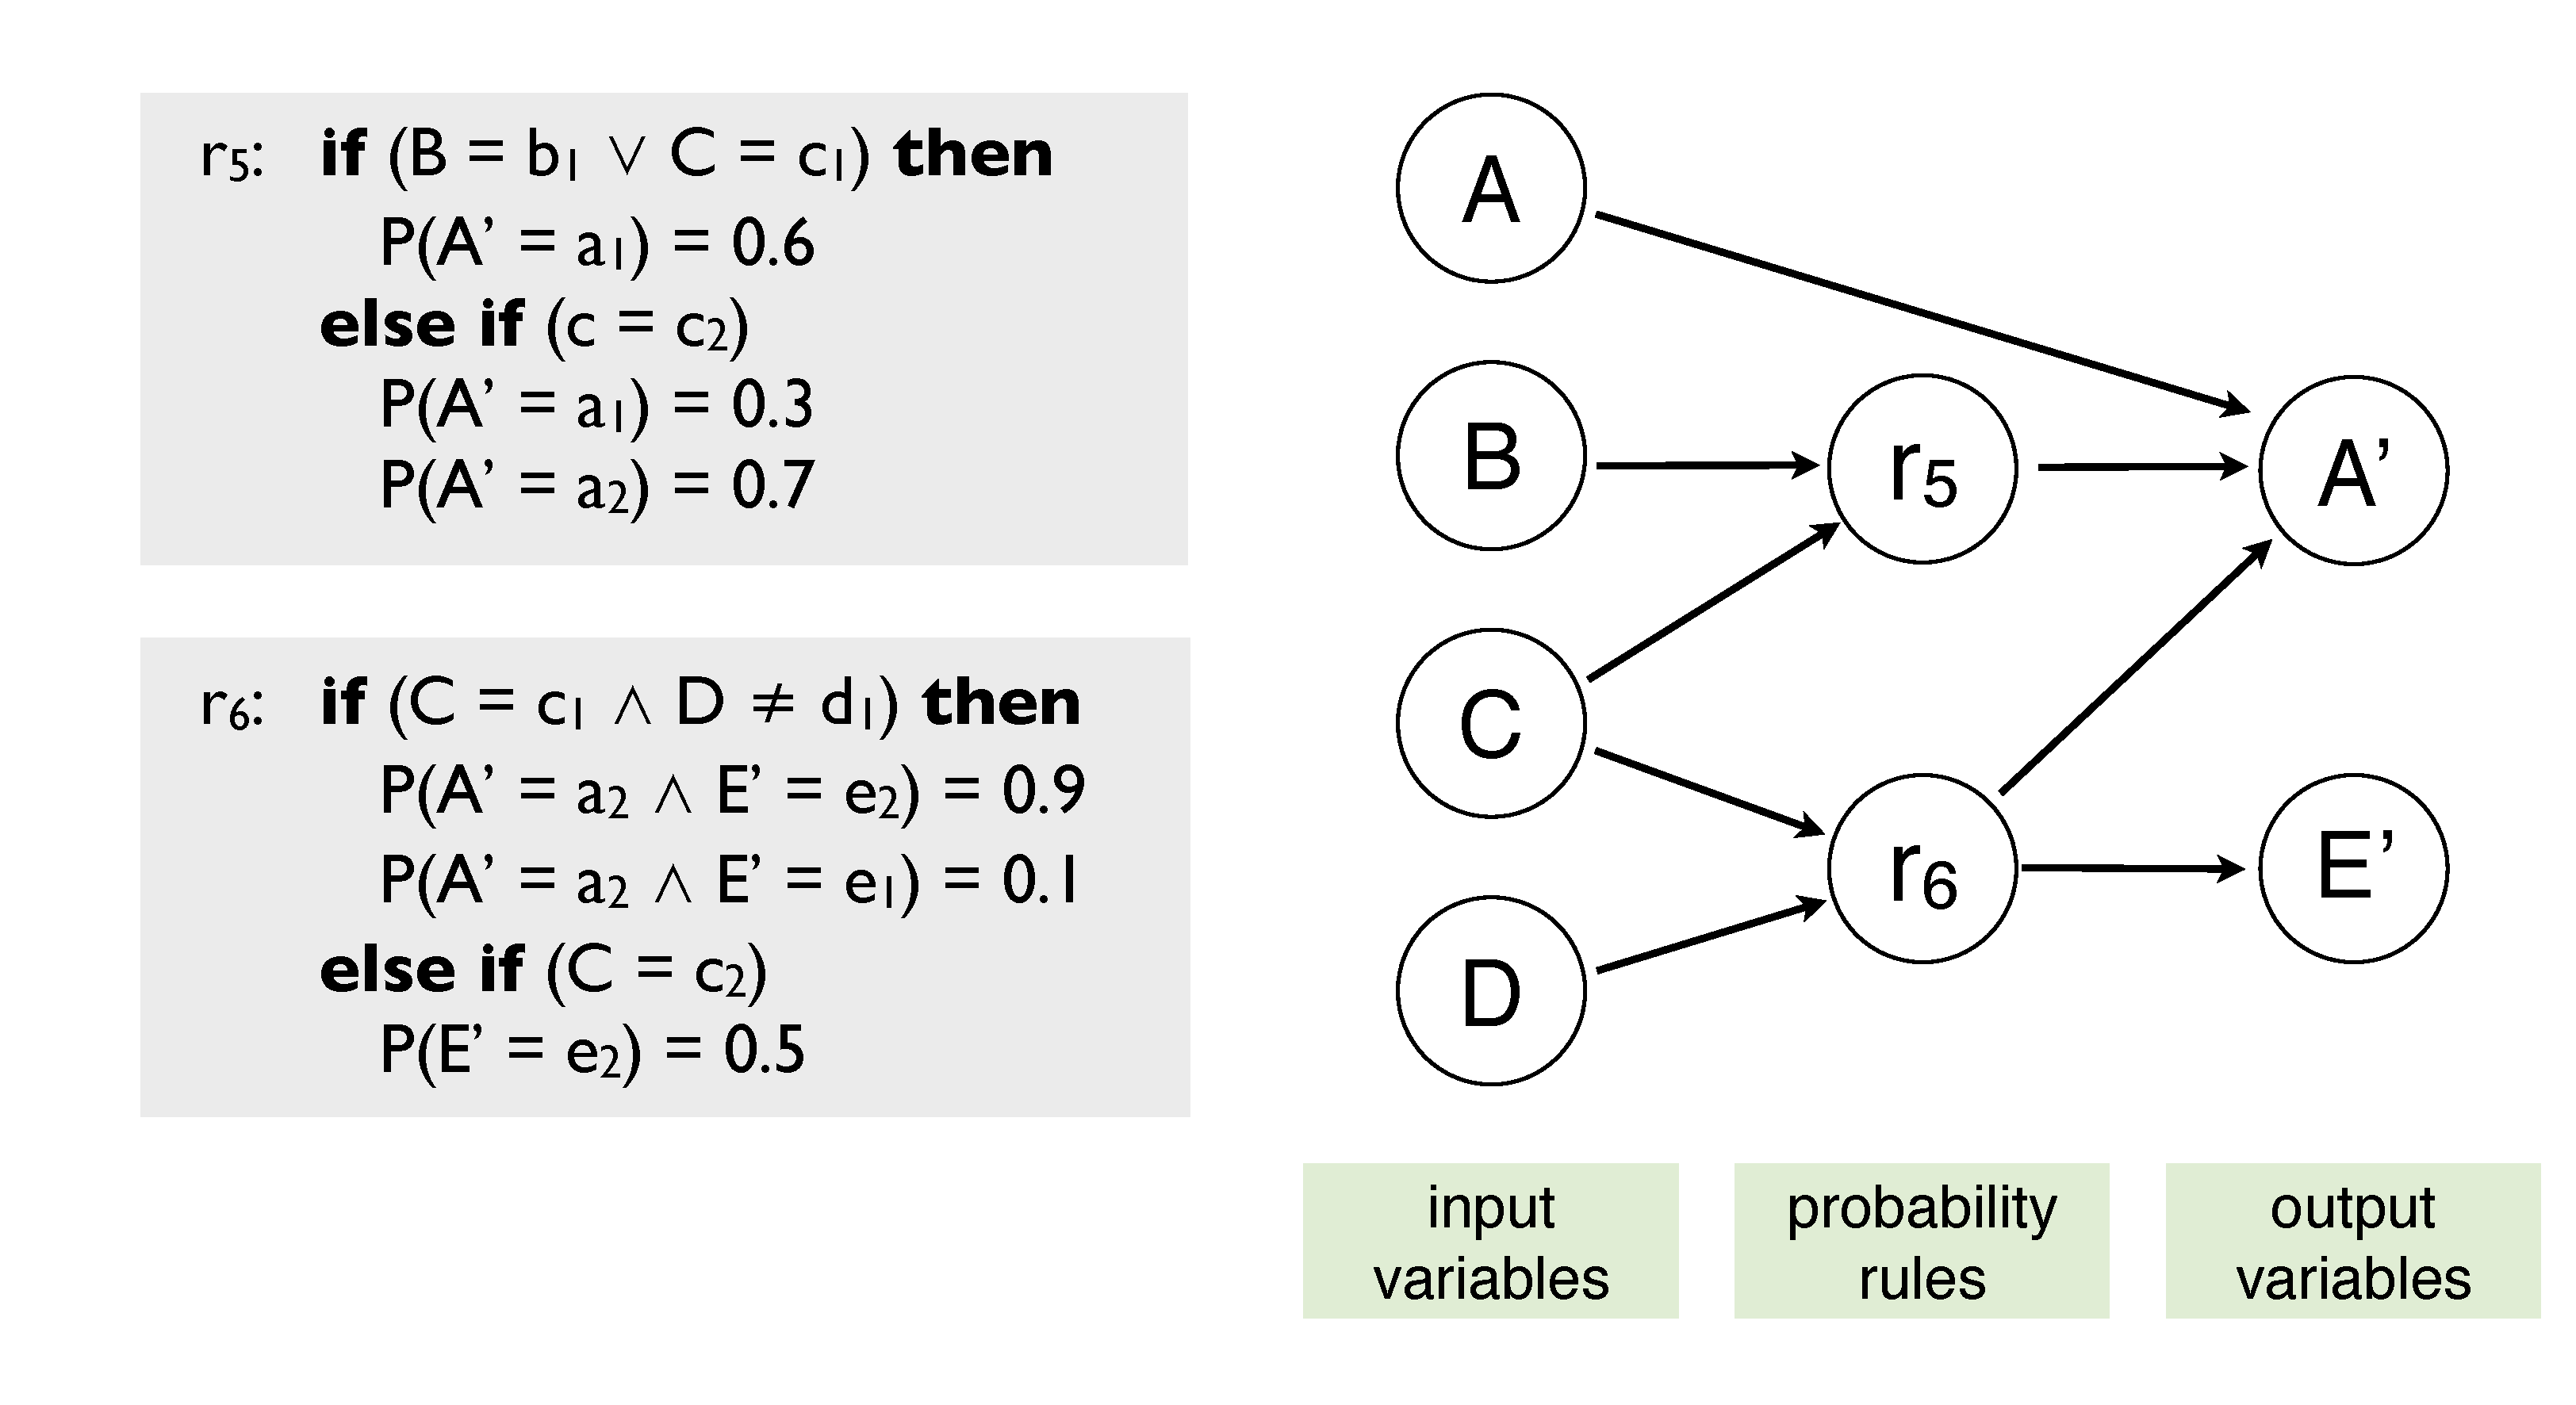
\includegraphics[scale=0.25]{imgs/ruleinstantiation.pdf}
\caption{Example of instantiation for the two probability rules $r_5$ and $r_6$. }
\label{fig:instantiationprob}
\end{figure}

The random variable represented by the node $r_5$ has three possible values, reflecting the effects described in the rule: $Val(r_5) = \{ \{A\!=\!a_1\}, \{A\!=\!a_2\}, \{\cdot\}\}$, where $\{\cdot\}$ denotes the empty effect.  Similarly, the random variable $r_5$ has four alternative effects: $Val(r_6) = \{\{A\!=\!a_2 \land E\!=\!e_2\}, \{A\!=\!a_2 \land E\!=\!e_1\}, \{E=e_2\}, \{\cdot\}\}$. 

We shall also adopt the following terminology to denote the probability distributions created through the instantiation procedure: 
\begin{itemize}
\item The conditional probability distribution associated with rule nodes such as $r_5$ and $r_6$ given their inputs is a \textit{rule distribution}.
\item The conditional probability distribution associated with output variables such $A'$ and $E'$ given the rule nodes that determine it is an \textit{output distribution}.
\end{itemize}

\subsubsection*{Rule distributions}

The rule distributions directly reflect the rule semantics.  Formally, the conditional probability distribution of a rule node $r$ given its input variables $I_1,...I_k$ is defined as: 
\begin{align}
& P(r\!=\!e \, | \, I_1\!=\!i_1,... I_k\!=\!i_k) = P(E_i = e) \label{eq:ruledistrib}
 \\ 
& \; \; \; \; \; \; \; \; \text{ where } i = \min_i (c_i \text{ is satisfied with } I_1\!=\!i_1 \land ... I_k\!=\!i_k) \nonumber 
\end{align}
Formally speaking, a condition $c_i$ is said to be satisfied iff the input assignment logically entails that the condition is true, that is :$(I_1\!=\!i_1 \land ... I_k\!=\!i_k) \vdash c_i$. The rule conditions are checked in sequential order until one condition is found to be satisfied. The rule distribution is then simply determined as the effect distribution $P(E_i\!=\!e)$ associated with the first satisfied condition $c_i$.  As the last condition $c_n$ corresponds to the final \textbf{else} block and is therefore always trivially true, there will always be at least one satisfied condition. 

As an example, the rule distribution $P(r_5 \, | \, B\!=\!b_1, C\!=\!c_1)$ for the node $r_5$ in Figure \ref{fig:instantiationprob} is defined as:
\begin{itemize}
\item $P(r_5 = \{A\!=\!a_1\} \, | \, B\!=\!b_1, C\!=\!c_1) = 0.6$
\item  $P(r_5 = \{\cdot\} \, | \, B\!=\!b_1, C\!=\!c_1) = 0.4$
%\item $P(r_5 = \{A\!=\!a_2\} \, | \, B\!=\!b_1, C\!=\!c_1) = 0$
\end{itemize}
Similarly, the distribution $P(r_6 \, | \, C\!=\!c_1, D\!=\!d_1)$ is a distribution with the empty effect $\{\cdot\}$ assigned to a probability 1. 

\subsubsection*{Output distributions} 

An output node $X'$ is conditionally dependent on all the rule nodes that refer to the variable $X$ in their effects.  In addition, output nodes that correspond to the updated version of existing nodes (such as $A'$ in the example of Figure \ref{fig:instantiationprob}) also include a conditional dependence on these existing nodes. The output distribution is a reflection of the combination of effects specified in the parent rules. The conditional probability distribution $P(X'|r_1\!=\!e_1,...r_n\!=\!e_n)$ for an output variable $X'$ with $n$ incoming rule nodes is defined in the following manner:
\begin{align}
&P(X'\!=\!x' \, | \, r_1\!=\!e_1,... r_n\!=\!e_n) = \begin{dcases}
\frac{\sum_{v \in {\mathbf{e}(X)}} \mathbf{1}(x' = v)} { |\mathbf{e}(X)| } & \text{if } \mathbf{e}(X)\!\neq\!\emptyset \\
\mathbf{1}(x' = \mathit{None}) & \text{otherwise}
\end{dcases}
\label{eq:outputdist1}
\end{align}
where the following notation is used: \begin{itemize}
\item $\mathbf{e}$ is the conjunction of all effects, i.e. $\mathbf{e} = e_1 \land ... e_n$.  This conjunction can include more than one assigned value for a particular variable.
\item $\mathbf{e}(X)$ denotes the (possibly empty) list of values specified for the variable $X$ in $\mathbf{e}$. 
\item $\mathbf{1}(b)$ is the indicator function for the Boolean $b$, with $\mathbf{1}(b)=1$ if $b$ is true and $0$ otherwise.
\end{itemize}

Equation \eqref{eq:outputdist1} stipulates that the distribution for $X'$ will follow the values assigned in the effect(s) provided that at least one effect specifies a value for it. If the effects include conflicting assignments, the distribution is spread uniformly over the alternative values. If no effects $e_1,...e_n$ specifies a value for $X$ , the value for $X'$ is set to a default $None$ value with probability 1. 

If the node $X'$ is an update of an existing node $X$, the procedure remains essentially the same as for \eqref{eq:outputdist1}, except in the case where all the effects specify empty assignments for the variable. In such case, the distribution for $X'$ will fall back to the value defined for the existing node $X$ instead of being assigned a $\mathit{None}$ value:
\begin{align}
&P(X'\!=\!x' \, | \, r_1\!=\!e_1,... r_n\!=\!e_n, X\!=\!x) = \begin{dcases} 
\frac{\sum_{v \in {\mathbf{e}(X)}} \mathbf{1}(x' = v)} { |\mathbf{e}(X)| }  & \text{if } \mathbf{e}(X)\!\neq\!\emptyset \\
\mathbf{1}(x' = x) & \text{otherwise}
\end{dcases}\label{eq:outputdist2}
\end{align}

As an example, the output distribution $P(A' \, | \, r_5\!=\!\{\cdot\},r_6\!=\!\{A\!=\!a_2 \land E\!=\!e_2\}, A\!=\!a_3)$ in Figure \ref{fig:instantiationprob} results in a deterministic distribution with a unique value $a_2$ with probability 1, since $\mathbf{e}(A) = \{a_2\}$. If the two rules generate conflicting assignments, the probability mass is divided equally over the alternative values.\footnote{This uniform division of the probability mass reflects that, in the absence of further knowledge, all rules are assumed to have the same ``weight''. If two or more rules generate contradictory effects, there is therefore no way to tell which rule is to take precedence. This assumption could however be refined in the future by e.g. associating numerical weights to particular rules or specifying a dominance hierarchy between the rules.}   The output distribution $P(A' \, | \, r_5\!=\!\{A\!=\!a_1\},r_6\!=\!\{A\!=\!a_2 \land E\!=\!e_2\}, A\!=\!a_3)$ provides two alternative values for $A$: $\mathbf{e}(A) = \{a_1,a_2\}$. The output distribution is thus a uniform distribution with two values: $a_1$ and $a_2$, each with probability 0.5. Finally, if all effects are empty, the output distribution is a simple copy of the distribution for the existing variable: $P(A' \, | \, r_5\!=\!\{\cdot\},r_6\!=\!\{\cdot\}, A\!=\!a_3)$ has a unique value $a_3$ with probability 1. 

Output distributions are directly derived from the effects in the rule nodes and are thus entirely parameter-free.  The ordering of the parent rules in the conditional probability distribution is arbitrary. The resulting distribution bears resemblance to the probabilistic Independence of Causal Influence (pICI) described by \cite{diez06}. 


\subsubsection*{Instantiation algorithm} 
\label{sec:utilruleinstantiation}

The procedure for instantiating a rule in a given dialogue state is detailed in Algorithm \ref{algo:instantiateProbRule}. 

\begin{algorithm}[h!]
\caption{: \textsc{InstantiateProbRule} ($\mathcal{B}, \mathit{r}$)}
\begin{algorithmic}[1] \vspace{1mm}
\REQUIRE Bayesian network $\mathcal{B}$ for the current state
\REQUIRE Probability rule $\mathit{r}$ to instantiate in network  \vspace{1mm}
\STATE $I_1,...I_k \leftarrow$ input variables for $\mathit{r}$
\STATE Create chance node $r$ with the rule distribution in Eq. \eqref{eq:ruledistrib}
\STATE Add node $r$ and dependency edges $I_1,...I_k \rightarrow r$ to $\mathcal{B}$ 
\IF {$Val(r) = \{\cdot\}$}
\STATE Prune $r$ from $\mathcal{B}$
\ELSE
\STATE $O_1,...O_l \leftarrow$ output variables mentioned in the effects of $r$
\FORALL {variable $O \in O_1,...O_l$}
\IF {$O'$ not already in $\mathcal{B}$}
\STATE Create chance node $O'$ with the output distribution in Eq. \eqref{eq:outputdist1}-\eqref{eq:outputdist2}
\STATE Add node $O'$ and (in case $O$ exists) dependency edge $O \rightarrow O'$ to $\mathcal{B}$
\ENDIF
\STATE Add dependency edge $r \rightarrow O'$ to $\mathcal{B}$ 
\ENDFOR
\ENDIF
\end{algorithmic}
\label{algo:instantiateProbRule}
\end{algorithm}

The first steps of the instantiation process are to extract in the Bayesian network the input variables of the rule (line 1), create a node corresponding to the rule (line 2) and include its dependency edges in the network (line 3).  The algorithm then checks whether at least one effect in $r$ is non-empty given its conditional dependences (lines 4).  If all effects are empty, the rule node is irrelevant and can be directly pruned (line 5). Otherwise, the output variables are extracted (line 7), and output nodes that do not already exist in the network are created (line 10-11). The final step is to establish dependency edges between the rule node and these output variables (line 13).


\subsection{Utility rules}

Utility rules are instantiated in the Bayesian network according to a similar procedure, with two notable differences compared to probability rules: \begin{itemize}
\item As utility rules define utility distributions, their instantiation correspond to utility nodes instead of chance nodes.
\item Instead of output variables, the rules are associated with decision variables.  The association direction is inverted, as the decision node must be input to the utility node.
\end{itemize} 

The result of the instantiation process is a decision network that incorporates chance nodes (corresponding to the state variables), utility nodes (corresponding to the utility rules) and associated decision nodes. Figure \ref{fig:instantitionutil} illustrates the instantiation of two utility rules $r_7$ and $r_8$. 

\begin{figure}[h]
\centering
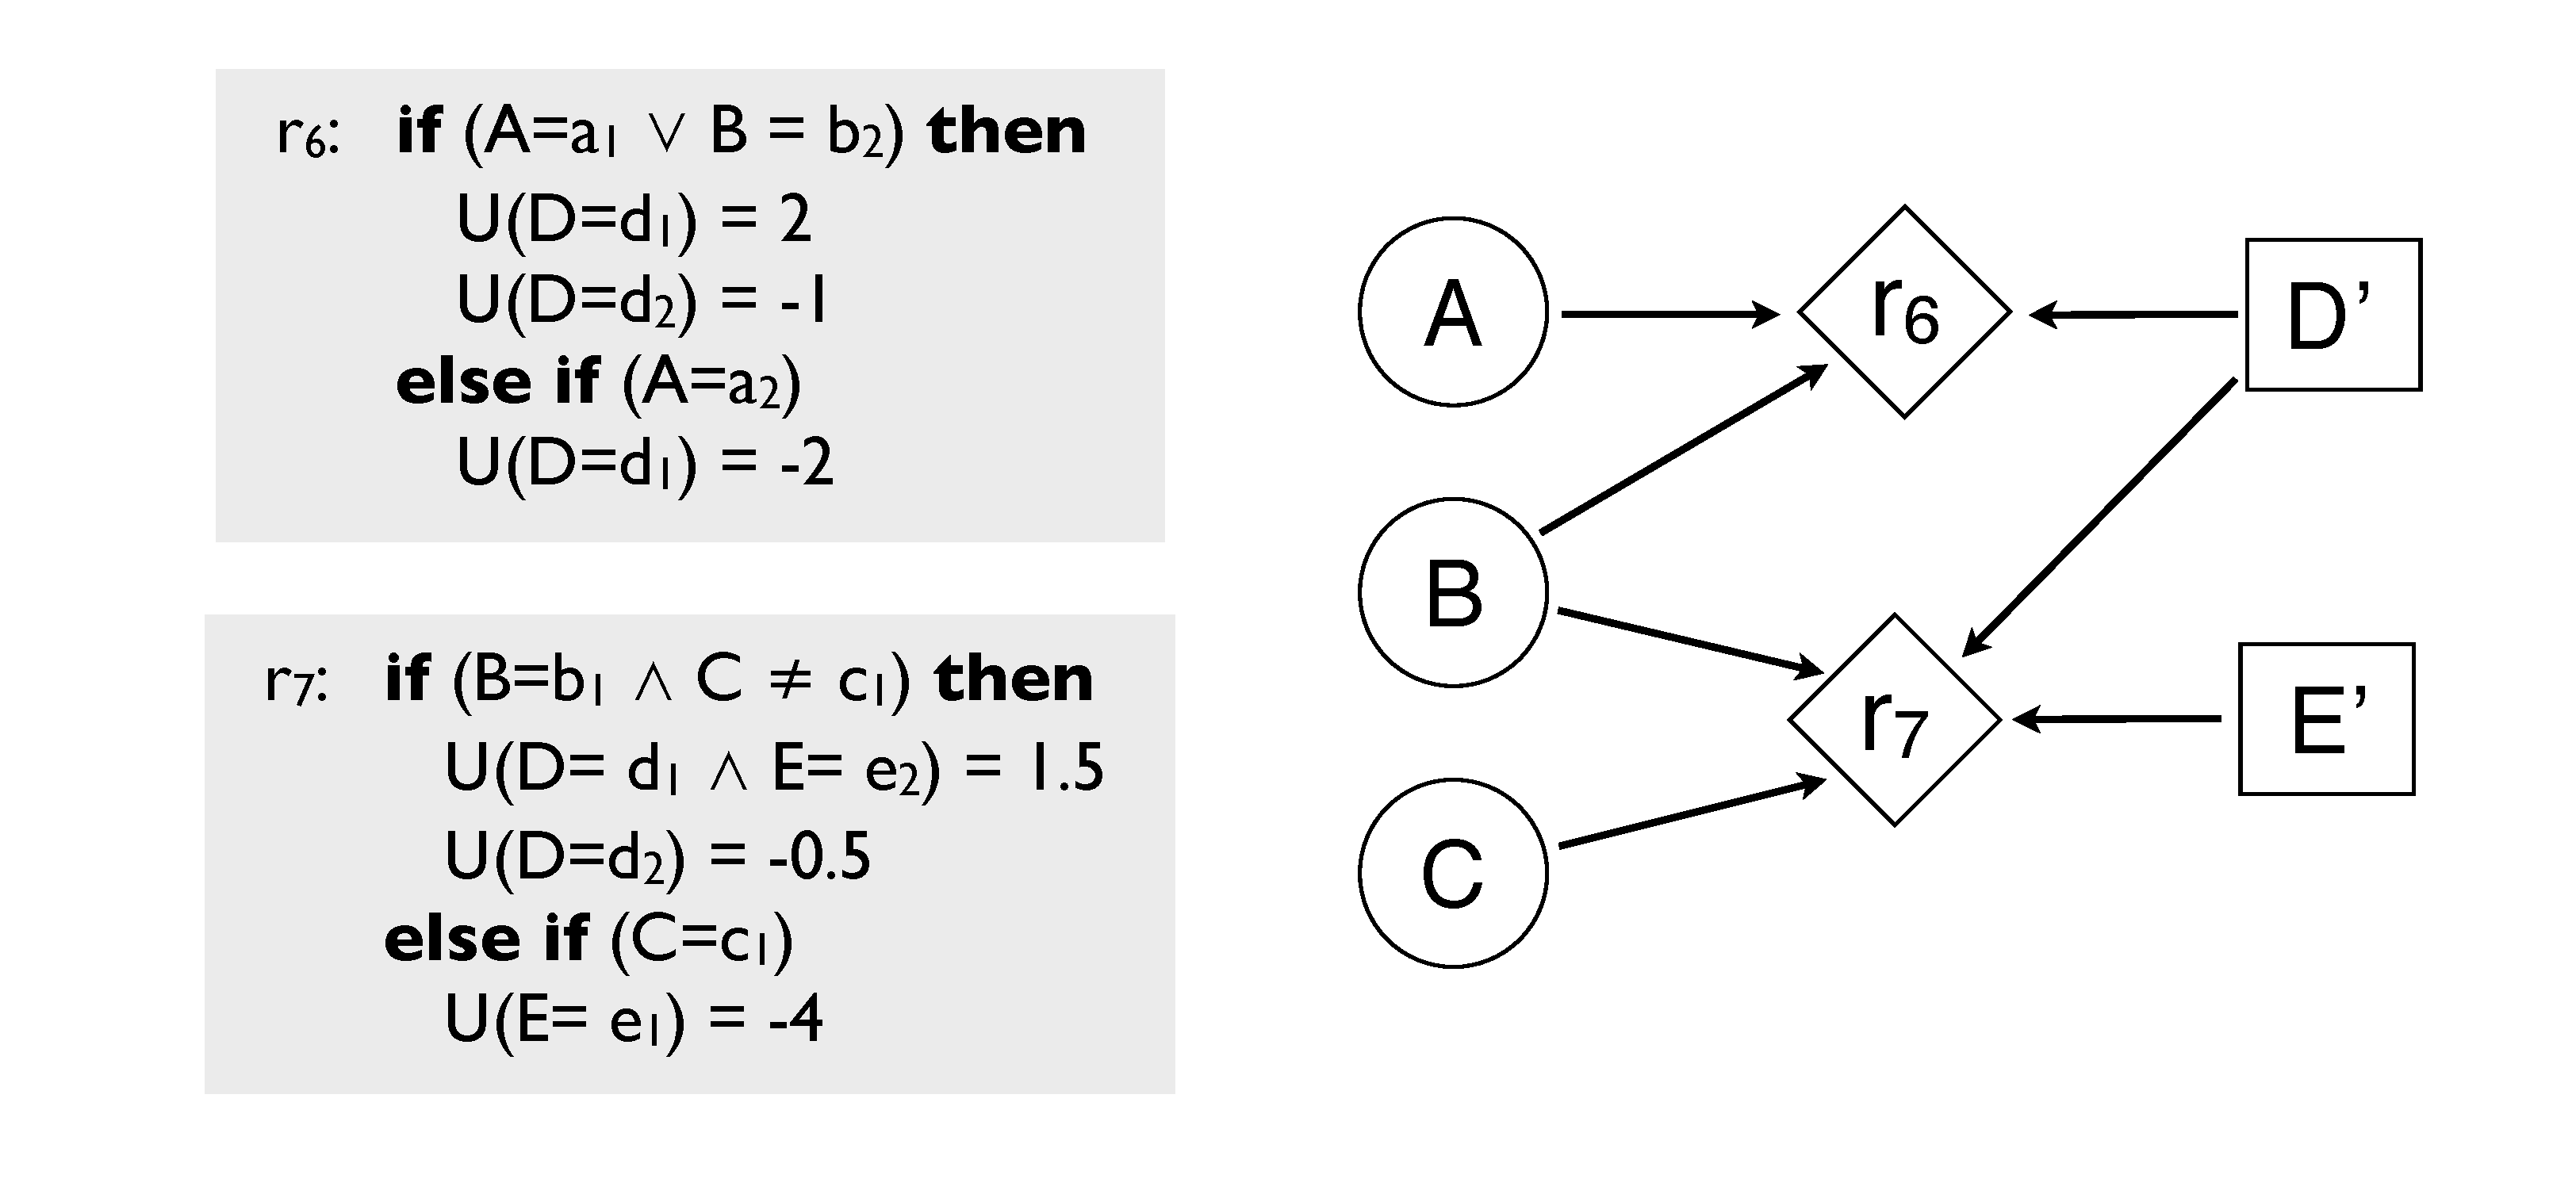
\includegraphics[scale=0.25]{imgs/ruleinstantiation2.pdf}
\caption{Example of instantiation for the two utility rules $r_7$ and $r_8$.}
\label{fig:instantitionutil}
\end{figure}


The utility distribution associated with each rule is a direct translation of the  \textit{if ... then ... else} rule.  Formally, the utility distribution generated by a rule $r$ with input variables $I_1,...I_k$ and decision variables $A_1,...A_l$ is defined as:
\begin{align}
& U_r(I_1\!=\!i_1,... I_k\!=\!i_k, A_1\!=\!a_1,... A_l\!=\!a_l) = U_i(A_1\!=\!a_1 \land... A_l\!=\!a_l) \label{eq:utildistrib}\\
&  \; \; \; \; \; \; \; \;  \; \; \; \text{ where } i = \min_i (c_i \text{ is satisfied with } I_1\!=\!i_1 \land ... I_k\!=\!i_k) \nonumber
\end{align}

If no utility is explicitly specified for $A_1\!=\!a_1 \land... A_l\!=\!a_l$, the default value is zero. 

As is conventionally assumed in decision networks, the total utility for a given assignment of decision variables is defined as the \textit{sum} of all utilities.  In case $A\!=\!a_1$, $B=\!=\!b_1$ and $C\!=\!c_1$, we can therefore calculate the total utility for the actions $D'\!=\!d_1 \ \land \ E'\!=\!e_1$ to be equal to $2 - 4 = -2$. 


\subsubsection*{Instantiation algorithm} 

The procedure for instantiating a utility rule is similar in most respects to the one already outlined for probability rules. Algorithm \ref{algo:instantiateUtilRule} details the procedure, starting from the extraction of the input variables, the creation of the rule node, and the inclusion of conditional dependences (line 1-3). The algorithm then checks if the utility distribution stipulates a non-zero utility for at least one decision (line 4).  If the answer is negative, the node is essentially irrelevant and can be pruned (line 5).  The decision variables associated with the rule are extracted (line 7), and a corresponding decision node is created if it does not already exists (line 10). Finally, the possible values specified for the decision variable are integrated to the node (line 12), and a dependency edge is established between the decision node and the utility node for the rule (line 13). 

\begin{algorithm}[h!]
\caption{: \textsc{InstantiateUtilRule} ($\mathcal{B}, \mathit{r}$)}
\begin{algorithmic}[1] \vspace{1mm}
\REQUIRE Bayesian network $\mathcal{B}$ for the current state
\REQUIRE Utility rule $\mathit{r}$ to instantiate in network  \vspace{1mm}
\STATE $I_1,...I_k \leftarrow $ input variables for $rule$
\STATE Create utility node $r$ with the utility distribution in Eq. \eqref{eq:utildistrib}
\STATE Add node $r$ and dependency edges $I_1,...I_k \rightarrow r$ to $\mathcal{B}$ 
\IF {utility distribution is empty for all inputs}
\STATE Prune $r$ from $\mathcal{B}$
\ELSE
\STATE $A_1,...A_l \leftarrow$ decision variables mentioned in the effects of $r$
\FORALL {variable $A \in A_1,...A_l$}
\IF {$A'$ not already in $\mathcal{B}$}
\STATE Create decision node $A'$ and add it to $\mathcal{B}$
\ENDIF
\STATE Add in $Val(A')$ the action values specified in the effects of $r$
\STATE Add dependency edge $A' \rightarrow r$ to $\mathcal{B}$ 
\ENDFOR
\ENDIF
\end{algorithmic}
\label{algo:instantiateUtilRule}
\end{algorithm}

\subsection{Quantification}
\label{sec:applicationquantif}

We saw in Section \ref{sec:quantification} that conditions and effect could include universally quantified variables, but have not yet discussed how such underspecified rules could be practically instantiated in the Bayesian network. The general instantiation principle remains unchanged: to each rule corresponds a distinct rule node responsible for the mapping between input and output variables (or decision variables for utility rules). The instantiation procedure must be however extended to accommodate the presence of quantified variables.  The key idea is to find all relevant \textit{groundings} for the quantified variables, and then calculate the effect distribution for each grounding. This method of handling quantifiers by extracting all possible groundings and reasoning at the propositional level is an instance of \textit{ground inference} \citep{getoor:srlbook07}. 

\subsubsection*{Extraction of input variables}

Universally quantified rules may underspecify both the names and values of random variables, as we saw in the examples of Section \ref{sec:quantification}.  Rule $r_3$ includes for instance a reference to an underspecified random variable $\mathit{shape}(y)$.  In order to instantiate the rule, the system must therefore first determine all random variables included in the model that match the underspecified description. If rule $r_3$ is instantiated on a state containing two objects $o_1$ and $o_2$, the resulting input variables will therefore be $\mathit{shape}(o_1)$ and $\mathit{shape}(o_2)$. 

Algorithm \ref{algo:getinputvariables} outlines how this search for matching input variables can proceed. The first step is to extract the initial input variables associated with the rule, which may include underspecified descriptions such as $\mathit{shape}(y)$. The algorithm then loops on each underspecified description to find possible groundings in the random variables of the Bayesian network.  The final result corresponds to the combination of the fully specified input variables for the rule and the groundings for the underspecified variables.  

\begin{algorithm}[h!]
\caption{: \textsc{GetInputVariables} ($\mathcal{B}, \mathit{r}$)}
\begin{algorithmic}[1] \vspace{1mm}
\REQUIRE Bayesian network $\mathcal{B}$ for the current state
\REQUIRE Probability or utility rule $\mathit{r}$ \vspace{1mm}
\STATE $\mathcal{I}_{r} \leftarrow $ Initial (possibly underspecified) input variables for $\mathit{r}$
\STATE $\mathcal{U}_{r} \leftarrow $ Subset of variable names in $\mathcal{I}_{r}$ that are underspecified
\STATE $\mathcal{G}_{r} \leftarrow$ Set of possible groundings for $\mathcal{U}_{r}$, initially empty
\FOR {underspecified variable name $u \in \mathcal{U}_{r}$}
\FOR {random variable $X$ in $\mathcal{B}$}
\IF {$X$ matches $u$}
\STATE $\mathcal{G}_{r} \leftarrow \mathcal{G}_{r} \cup [X]$
\ENDIF
\ENDFOR
\ENDFOR
\RETURN $(\mathcal{I}_{r} \ / \ \mathcal{U}_{r}) \ \cup \  \mathcal{G}_{r}$
\end{algorithmic}
\label{algo:getinputvariables}
\end{algorithm}

 %Line 1 in Algorithms \ref{algo:instantiateProbRule} and \ref{algo:instantiateUtilRule} is then replaced by: 
%\begin{algorithmic}[1] \vspace{1mm}
%\STATE $I_1,...I_k \leftarrow $ \textsc{GetInputVariables} ($\mathcal{B}, \mathit{r}$)
%\end{algorithmic}


\subsubsection*{Extraction of relevant groundings}

Once the input variables for the rules are retrieved, the next step is to establish the set of relevant groundings $G$ for the universally quantified variables.  The groundings are always determined relative to a particular assignment of values for the (grounded) input variables $I_1,...I_k$.

Given an input assignment $\{I_1\!=\!i_1 \land ... I_k\!=\!i_k\}$, the set of groundings $G$ are derived in a heuristic manner, by checking which ground terms (constants and functions of constants) from the input assignment can function as proper substitutions for the quantified variables.  These ground terms define the domain of discourse for the application of the universal quantifier. The collection of relevant ground terms is then combined into subsets of size $p$, where $p$ corresponds to the number of universally quantified variables $\mathbf{y} = y_1, ... y_p$. These combinations form the groundings $G$ for the input assignment. 


%The groundings are always determined relative to a particular assignment of values for the input variables. Given such input assignment, the groundings are defined as substitutions of quantified variables to ground terms that result in the satisfaction of at least one condition. Let us assume a rule with input variables $I_1,...I_k$ and quantified over $\mathbf{y}$. Given a particular assignment for the input variables $I_1,...I_k$, each condition $c_i$ is checked to find the possible groundings of its quantified variables that lead to the satisfaction of the condition.\footnote{The search for possible groundings is limited to a set of ground terms (constants and functions of constants) determined in a heuristic manner, based on the ground terms used in the parent variables of the rule node.}  The number of groundings can be zero if the condition cannot be satisfied. As illustrated in Algorithm \ref{algo:getgroundings}, the result of this process is a set of groundings $G$ that leads to the satisfaction of at least one condition when substituted to the quantified variables in this condition. The expression $\phi[a/b]$ denotes (as in formal logic) the formula $\phi$ where all instances of $a$ are substituted by $b$.

% specified in the input assignment. For instance, the assignment $\mathit{shape}(o_1)\!=\!\mathit{sphere} \land \mathit{shape}(o_1)\!=\!\mathit{cone}$ includes a total of six ground terms: $o_1$, $o_2$, $\mathit{sphere}$, $\mathit{cone}$, $\mathit{shape}(o_1)$ and $\mathit{shape}(o_1)$.
 
% For instance, the assignment $\mathit{shape}(o_1)\!=\!\mathit{sphere} \land \mathit{shape}(o_1)\!=\!\mathit{cone}$ includes 6 ground terms: $o_1$, $o_2$, $\mathit{sphere}$, $\mathit{cone}$, $\mathit{shape}(o_1)$ and $\mathit{shape}(o_1)$.

 %The possible groundings for a given input must be in this setting restricted to a finite set. In order to retain tractability, the maximum number of groundings is also capped by a threshold.
 %Groundings that satisfy a condition leading to an empty effect can be discarded. 
 
%\begin{algorithm}[h!]
%\caption{: \textsc{GetGroundings} ($\mathit{r}, \{I_1\!=\!i_1 \land ... I_k\!=\!i_k\}$)}
%\begin{algorithmic}[1] \vspace{1mm}
%\REQUIRE $\mathit{r}$: Probability or utility rule 
%\REQUIRE $\{I_1\!=\!i_1 \land ... I_k\!=\!i_k\}$ assignment for the parent variables of the rule  \vspace{1mm}
%\STATE $G \leftarrow \emptyset$
%\FORALL {condition $c_i$ in $\mathit{r}$}
%\STATE Let $\mathbf{y}_i \subset \mathbf{y} $ be the quantified variables present in $c_i$
%\STATE $G_i \leftarrow \{\text{groundings } \mathbf{g} $ such that $ \ c_i [\mathbf{y}_i / \mathbf{g} ] \text{ is satisfied with } I_1\!=\!i_1 \land ... I_k\!=\!i_k \}$
%\STATE $G \leftarrow G \cup G_i$
%\ENDFOR
%\RETURN $G$
%\end{algorithmic}
%\label{algo:getgroundings}
%\end{algorithm}


\subsubsection*{Quantified probability rules}

As we have seen, probability rules are instantiated as chance nodes associated with a rule distribution.  For rules containing universal quantifiers, each grounding in $G$ gives rise to a particular distribution over effects.  The instantiation procedure generates a distinct effect distribution for each grounding $\mathbf{g}_j$: 
\begin{align}
& P(r_{\mathbf{g}_j}\!=\!e' \, | \, I_1\!=\!i_1,... I_k\!=\!i_k) = P(E_i = e) \label{eq:quantifruledistrib}
 \\
& \; \; \; \; \; \; \; \; \text{where } i = \min_i (c_i[\mathbf{y} / \mathbf{g}_j]\text{ is satisfied with } I_1\!=\!i_1 \land ... I_k\!=\!i_k) \nonumber \\ 
& \; \; \; \; \; \; \; \; \text{and } e' = e [\mathbf{y} / \mathbf{g}_j] \nonumber
\end{align}

The expression $\phi[a/b]$ denotes (as in formal logic) the formula $\phi$ where all instances of $a$ are substituted by $b$.

Empty and redundant effect distributions are discarded. The grounding procedure results in a  collection of distributions $ \langle P(r_{\mathbf{g}_1}),... P(r_{\mathbf{g}_p}) \rangle$.    The final conditional probability distribution for the rule node is then defined as the joint distribution over these grounding-specific distributions: 
\begin{align}
& P(r\!=\![e_1 \land ... e_{q}] \, | \, I_1\!=\!i_1,... I_k\!=\!i_k) = \prod_{j=1}^{q} P(r_{\mathbf{g}_j}\!=\!e_j)
\end{align}

Figure \ref{fig:quantinstantitionprob} shows how the rule $r_3$ is instantiated in a state with two objects $o_1$ and $o_2$, each associated with a random variable describing its shape.

\begin{figure}[h]
\centering
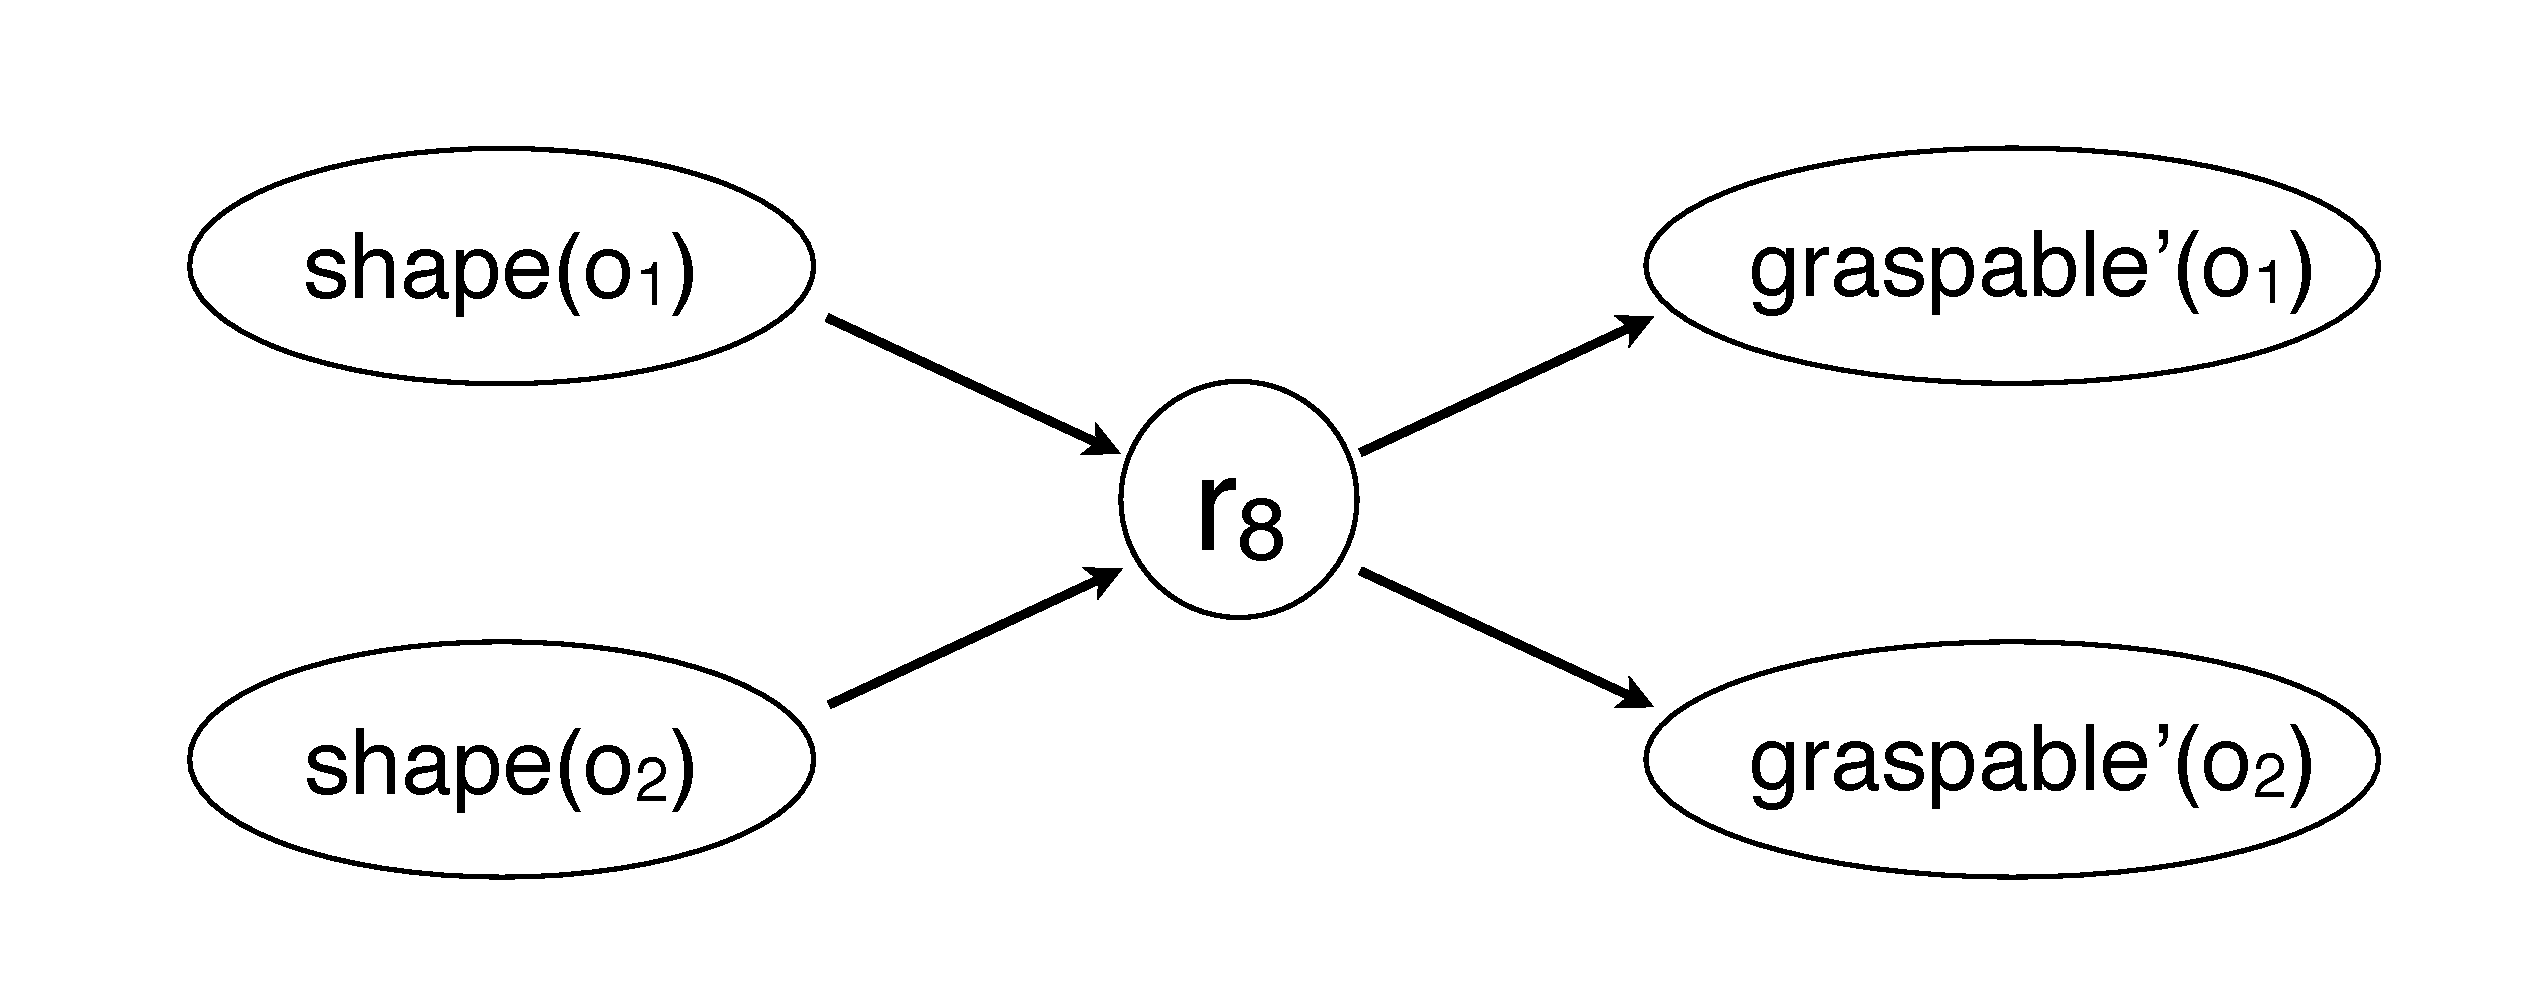
\includegraphics[scale=0.25]{imgs/quantruleinstantiation.pdf}
\caption{Instantiation of the probability rule $r_3$ on a state with two objects $o_1$ and $o_2$.}
\label{fig:quantinstantitionprob}
\end{figure}

As an example, the probability distribution $P(r_3 \, | \, \mathit{shape}(o_1)\!=\!\mathit{sphere}, \mathit{shape}(o_2)\!=\!\mathit{cone})$ has two relevant groundings $y\!=\!o_1$ and $y\!=\!o_2$, from which four alternative effects are derived: \begin{itemize}
\item $\{\mathit{graspable}(o_1)\!=\!true \land \mathit{graspable}(o_2)\!=\!true \} $ with probability $0.9 \times 0.2 = 0.18$ 
\item $\{\mathit{graspable}(o_1)\!=\!true \land \mathit{graspable}(o_2)\!=\!false\}$ with probability $0.9 \times 0.8 = 0.72$ 
\item $\{\mathit{graspable}(o_1)\!=\!false \land \mathit{graspable}(o_2)\!=\!true \}$ with probability $0.1 \times 0.2 = 0.02$ 
\item $\{\mathit{graspable}(o_1)\!=\!false \land \mathit{graspable}(o_2)\!=\!false\}$ with probability $0.1 \times 0.8 = 0.08$. 
\end{itemize} 

The effects specified for $r_3$ mention two output variables: $\mathit{graspable}(o_1)$ and $\mathit{graspable}(o_1)$.  These two variables are thus created as children of the node $r_3$. 

\subsubsection*{Quantified utility rules}

Utility rules can be similarly extended to accommodate quantified variables. As for probability rules, the instantiation of universally quantified utility rules proceeds by determining a set of groundings and generating a particular utility distribution for each.\footnote{The extraction of groundings is slightly modified for utility rules in order to integrate the ground terms appearing in both the input and decision assignments.}
 For a utility rule with input variables $I_1,...I_k$, decision variables $A_1,...A_l$ and quantified variables $\mathbf{y}$,
 
 \begin{align}
& U_{\mathbf{g}_j}(I_1\!=\!i_1,... I_k\!=\!i_k, A_1\!=\!a_1',... A_l\!=\!a_l') = U_i(A_1\!=\!a_1 \land... A_l\!=\!a_l) 
 \\
& \; \; \; \; \; \; \; \;   \; \; \;\text{where } i = \min_i (c_i[\mathbf{y} / \mathbf{g}_j]\text{ is satisfied with } I_1\!=\!i_1 \land ... I_k\!=\!i_k) \nonumber \\
& \; \; \; \; \; \; \; \;   \; \;  \text{and } a_1' = a_1[\mathbf{y} / \mathbf{g}_j], ... \ \ a_l' = a_l[\mathbf{y} / \mathbf{g}_j] \nonumber
\end{align}

After discarding empty and redundant distributions, the result is a set of utility distributions $ \langle U_{\mathbf{g}_1},... U_{\mathbf{g}_p} \rangle$. The total utility distribution for the rule is then constructed by adding up the grounding-specific utility distributions:   
\begin{align}
& U_{r}(I_1,... I_k, A_1\,... A_l) = \sum_{j=1}^{q} U_{\mathbf{g}_j}(I_1,... I_k, A_1,... A_l) \label{eq:quantifruledistrib}
\end{align}


The result of instantiating rule $r_4$ on a state with two objects $o_1$, $o_2$ with associated random variables $\mathit{graspable}(o_1)$ and $\mathit{graspable}(o_2)$ is shown in Figure  \ref{fig:quantinstantitionutil}.  

\begin{figure}[h]
\centering
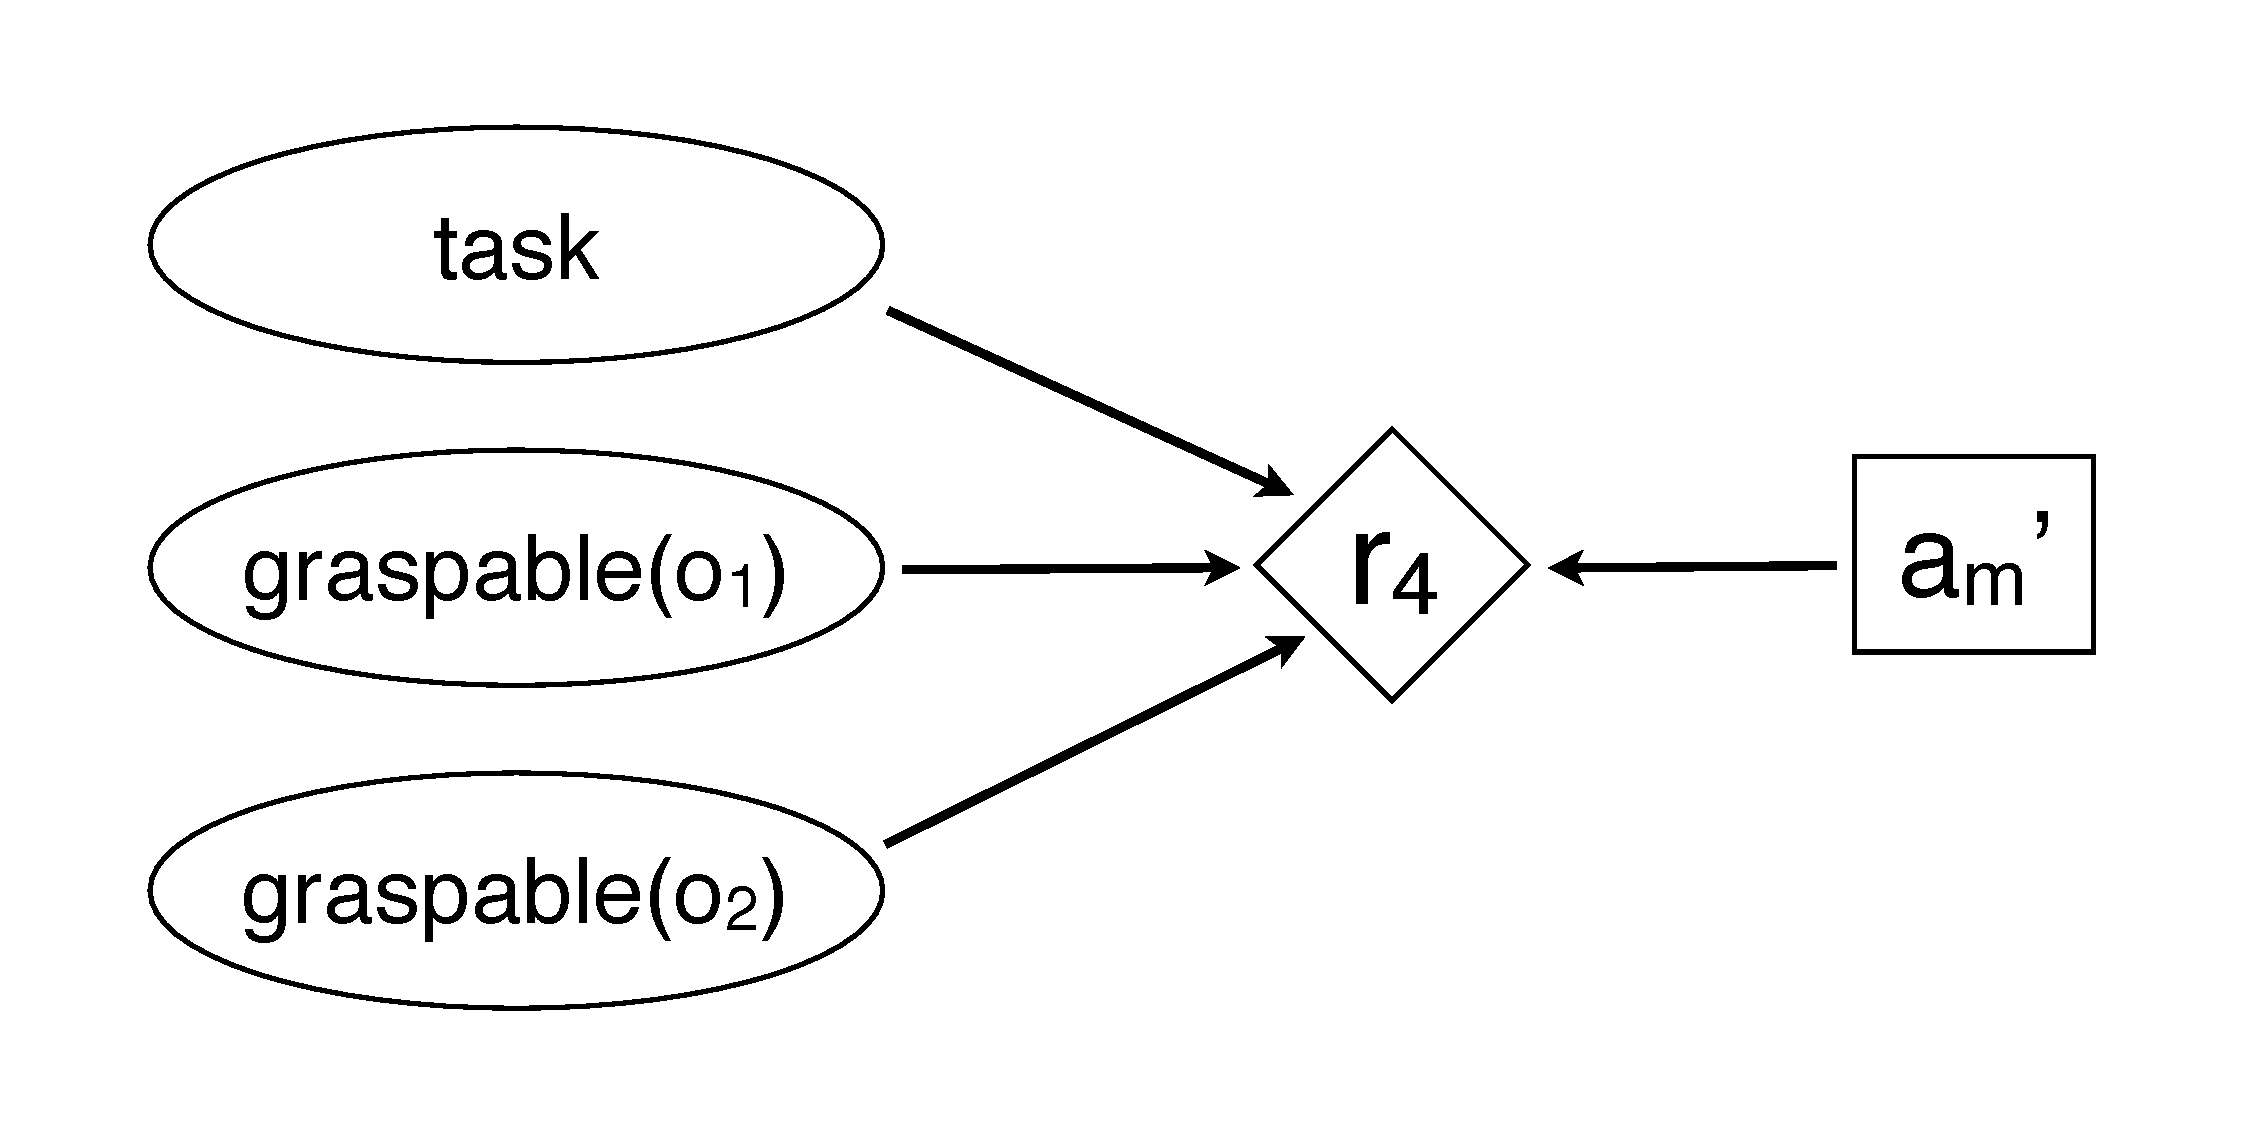
\includegraphics[scale=0.25]{imgs/quantutilruleinstantiation.pdf}
\caption{Instantiation of the quantified utility rule $r_9$ on a state with two objects $o_1$ and $o_2$.}
\label{fig:quantinstantitionutil}
\end{figure}

The utility distribution $U_{r_4}(\mathit{task}\!=\!\mathit{grasp}(o_1), \mathit{graspable}(o_1) \!=\!\mathit{true}, \mathit{graspable}(o_2)\!=\!\mathit{false}, a_m)$ assigns the action $a_m\!=\!\mathit{grasp}(o_1)$ to a utility of 2, while the action $a_m\!=\!\mathit{grasp(o_2)}$ is assigned to a utility of -2. 

\subsubsection*{Tractability aspects}

Although the use of universally quantifiers greatly improves the expressivity of probabilistic rules, they also tend to increase the in- and out-degrees of rule nodes (that is, the cardinality of their parents and children nodes). Approximate inference techniques are thus necessary to handle this conditional structure in a tractable manner. Sampling methods such as likelihood weighting have in practice proved to work well in this setting (cf. Section \ref{sec:inference}).

It should be stressed that the groundings are always extracted \textit{given a specific value assignment} for the input variables. By restricting the groundings to this limited domain of discourse, we ensure that the number of alternative effects remains bounded and avoid the generation of spurious effects.   This instantiation procedure was found to be much more efficient than copying the rule in distinct nodes, as investigated in earlier implementations of the formalism \citep{relational-apl2012}.  This procedure departs from other frameworks such as Markov Logic Networks, where the functions and predicates are duplicated for every possible grounding of variables in the domain \citep{Richardson:2006}.


 %In order to keep the number of groundings under control, the specification of probabilistic rules should nevertheless refrain from introducing more universally quantified variables than necessary.

%

\section{Processing workflow}
\label{sec:processing-workflow}

The two previous sections detailed how probability and utility rules are internally defined, and how they can be instantiated as nodes of a graphical model. We are now ready to explain how collections of rules are practically applied at runtime to update the dialogue state and perform action selection. The general workflow is strongly inspired by information-state approaches to dialogue management \citep{Larsson:2000,Buckley:2006}, as the dialogue state serves as a central blackboard monitored by various groups of rules that are ``triggered'' upon relevant changes. 

The section first describes how dialogue domains are organised in collections of rules called ``models'', and then goes on to explain how these models are applied to update state variables and express the utility of particular actions. We also demonstrate the general processing workflow on a detailed example. 


\subsection{Domain representation}

Dialogue domains can consist of multiple probability and utility rules. These rules are internally grouped in collections of rules called \textit{models}. A model is simply a collection of rules that is associated with one or more ``trigger'' variables that specify when the model is to be instantiated. Each model is attached the dialogue state and monitors it to detect changes affecting their trigger variables. When these trigger variables are changed at runtime by another module, they lead to the instantiation of the model rules. Formally, a model $m$ is defined as a pair $\langle \mathcal{T}_m, \mathcal{R}_m \rangle$ where $\mathcal{T}_m$ corresponds to the trigger variables and $\mathcal{R}_m$ to the rules included in the model.

A dialogue domain is represented as a pair $\langle \mathcal{B}_0, \mathcal{M} \rangle$, where $\mathcal{B}_0$ is the initial dialogue state  and $\mathcal{M}$ the set of rule-based models attached to it. The organisation of rules into models allows the system designer to structure the application pipeline in a modular manner. Each model can be intuitively viewed as a distinct component responsible for a particular inference or decision step. 

Section \ref{sec:domain-specification} explains how dialogue domains (and the models that compose them) are practically encoded in the \opendial architecture, based on an XML specification. 

\subsection{Update algorithm} 

The software architecture adopted in this thesis takes the form of an event-driven, blackboard architecture \citep{jaspis2004,Buckley:2006} revolving around a dialogue state $\mathcal{B}$ represented as a Bayesian network.  As in information state approaches, this dialogue state is read and written by the various modules integrated in the dialogue system. 

The update procedure is shown in Algorithm \ref{algo:stateupdate}. The procedure is started upon the reception of new variables to incorporate in the state, such as new user inputs processed by the speech recognition and natural language understanding components. The first step is to insert the variables in the dialogue state and possibly relate them to their predicted values (lines 2-3). The algorithm then triggers the instantiation of the relevant domain models (line 4), leading to a recursive chain of updates.  If the expanded dialogue state contains decision and utility variables, the algorithms searches for the optimal action, selects it, and activates the models that are triggered as a result  (lines 6-8). Finally, the updated state is reduced by pruning away unnecessary nodes and incorporating the evidence (line 10). 


\begin{algorithm}[h]
\caption{: \textsc{UpdateState} ($\mathcal{B}, \mathbf{X}$)}
\begin{algorithmic}[1] \vspace{1mm}
\REQUIRE Bayesian network $\mathcal{B}$ for the current state
\REQUIRE New random variables $\mathbf{X}$ to insert in the state \vspace{1mm}
\STATE Initialise evidence $\mathbf{e} \leftarrow \emptyset$
\STATE Insert $\mathbf{X}'$ to the current state $\mathcal{B}$ 
\STATE $\mathcal{B}, \mathbf{e} \leftarrow $ \textsc{IntegratePredictions}($\mathcal{B}, \mathbf{e}, \mathbf{X}'$)
\STATE $\mathcal{B}, \mathbf{e} \leftarrow$ \textsc{TriggerModels} ($\mathcal{B}, \mathbf{e},  \mathbf{X}'$) \vspace{1mm}
\WHILE {$\mathcal{B}$ contains decision variables}
\STATE $\mathbf{a}^* \leftarrow $ \textsc{SelectAction} ($\mathcal{B}, \mathbf{e}$)
\STATE Assign $\mathbf{A}' = \mathbf{a}^*$
\STATE $\mathcal{B}, \mathbf{e} \leftarrow$ \textsc{TriggerModels} ($\mathcal{B}, \mathbf{e}, \mathbf{A}'$)
\ENDWHILE \vspace{1mm}
\STATE $\mathcal{B} \leftarrow \textsc{PruneState} (\mathcal{B}, \mathbf{e})$ \vspace{1mm}
\end{algorithmic}
\label{algo:stateupdate}
\end{algorithm}

We now describe each of these steps in detail.


\subsubsection*{Connecting predictions and observations}

Rules are sometimes used to provide predictions on variables that will be observed in the next time steps.\footnote{This is notably the case for the user action model $P(a_u \, | \, i_u, a_m)$, which estimate the relative probabilities for the next dialogue action from the user. The prediction provide a prior on the future observation of the user action.} In order to distinguish random variables that express a prediction on a future outcome from those that reflect an actual (although possibly uncertain) observation, we denote predictive variables with a subscript $p$. A variable $X_p$ represents therefore a random variable on the predicted values of the variable $X$ to be observed in the future. 

\begin{wrapfigure}[11]{r}{48mm}
\vspace{-2mm}
\centering
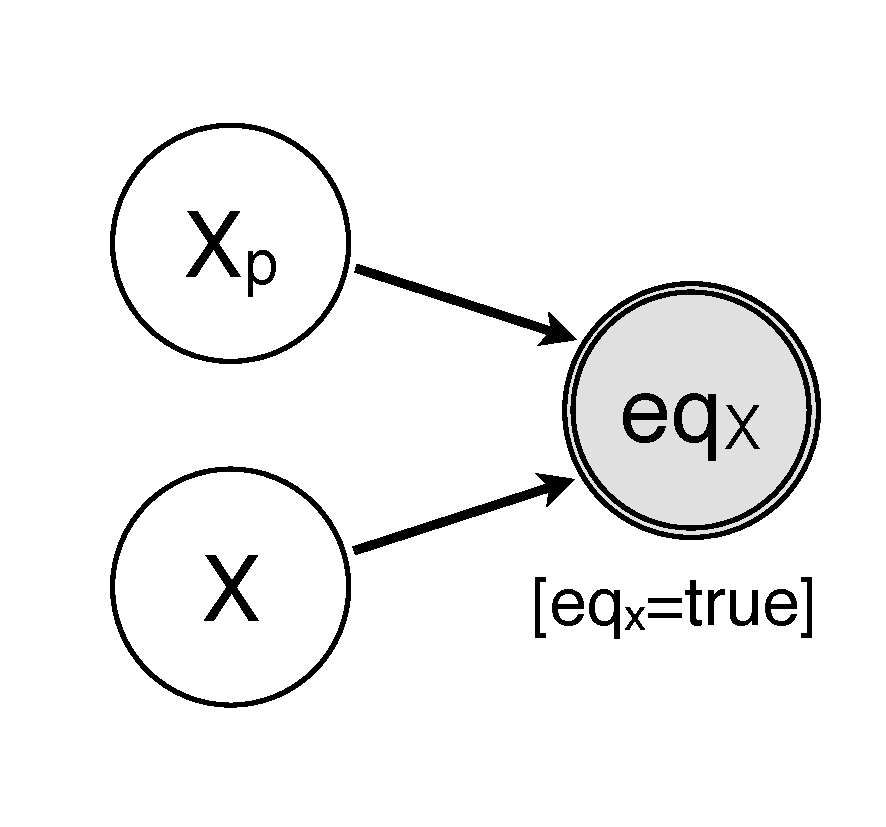
\includegraphics[scale=0.25]{imgs/prediction.pdf} 
\vspace{-2mm}
\caption{Equivalence node $eq_{X}$ with parents $X$ and $X_p$.}
\label{fig:prediction}
\end{wrapfigure}

Prediction and observation variables must be connected with one another at runtime.  In the case where the observation is known with certainty, this connection can simply be represented as an assignment of evidence values.  However, dialogue often include observations that are themselves uncertain and represent ``soft'' or virtual evidence.  Several techniques are available to practically encode this evidence. The method adopted in this thesis is to add a new boolean-valued chance node, subsequently called the \textit{equivalence node} $eq_{X}$, that is conditionally dependent on both $X$ and $X_p$, as shown in Figure \ref{fig:prediction}. The conditional probability distribution of $eq_X$ is deterministic (graphically depicted by a double circle around the chance node): 
\begin{equation}
P(eq_{X}\!=\!true \, | \, X\!=\!x, X_p\!=\!x_p) = \begin{cases}
1 & \text{if } x = x_p \\
0 & \text{otherwise}
\end{cases} \label{eq:equivdistrib}
\end{equation}

The use of a distinct node to express the evidence is motivated by the fact that $X$ and $X_p$ can have arbitrary incoming and outgoing edges with other variables. 

The assignment $eq_{X} \!=\! true$ is added to the evidence. The posterior distribution given the evidence allows the prediction to act as a prior for the observed distribution:
\begin{align}
&P(X = x \, | eq_{X}\!=\!true) \nonumber \\
&=  \alpha \ P(X\!=\!x)  \sum_{x_p \in Val(X_p)} P(eq_{X}\!=\!true | X\!=\!x, X_p \!=\!x_p ) P(X_p\!=\!x_p) \\
&= \alpha \ P(X\!=\!x) \ P(X_p\!=\!x) \label{eq:equivalence}
\end{align}

The inclusion of an equivalence node between $X$ and $X_p$ with evidence  $[eq_{X}\!=\!true]$ modifies the distribution of the variables $X$ and$X_p$ as well as their respective parents/children nodes.  Algorithm \ref{algo:integratepredictions} illustrates the process of integrating predictions for the variables $\mathit{Vars}$. 

\begin{algorithm}[h]
\caption{: \textsc{IntegratePredictions} ($\mathcal{B}, \mathbf{e}, \mathit{Vars}$)}
\begin{algorithmic}[1] \vspace{1mm}
\FORALL {$X \in \mathit{Vars}$}
\IF {there is a corresponding prediction variable $X_p \in \mathcal{B}$}
\STATE Create equivalence node $eq_{X}$ with distribution in Eq. \eqref{eq:equivdistrib}
\STATE Insert $eq_{X}$ in $\mathcal{B}$ with parents $\mathit{X}$ and $\mathit{X}_p$
\STATE Add assignment $[eq_{X}\!=\!true]$ to evidence $\mathbf{e}$
\ENDIF
\ENDFOR
\RETURN $\mathcal{B}, \mathbf{e}$
\end{algorithmic}
\label{algo:integratepredictions}
\end{algorithm}



\subsubsection*{Model instantiation}

After inserting the new variables in the dialogue state and connecting them to their predicted values, the next step in the processing workflow is to trigger the relevant domain models . 

Algorithm \ref{algo:triggerModels} summarises the steps involved in the instantiation of the domain models. The algorithm takes three arguments: a dialogue state $\mathcal{B}$ represented as a Bayesian network, an assignment of evidence values and a list of random variables that have been recently updated in the dialogue state. The algorithm loops on all domain models and instantiates the ones that are triggered by the updated variables. The rules are instantiated one by one, following the procedure we have outlined in the previous section. Once all models are traversed, the output variables of the instantiated rules become updated variables themselves, and the procedure is repeated until no more models can be applied.  To avoid the occurrence of infinite triggering cycles, models are limited to one instantiation per update. The algorithm returns both the dialogue state expanded with new variables, and the evidence assignment attached to the equivalence nodes. 


\begin{algorithm}[h]
\caption{: \textsc{TriggerModels} ($\mathcal{B}, \mathbf{e}, \mathit{UpdatedVars}$)}
\begin{algorithmic}[1] \vspace{1mm}
\WHILE {$\mathit{UpdatedVars} \neq \emptyset$}
\STATE $\mathit{NewVars} \leftarrow \emptyset$
\FORALL {models $m$}
\IF {$\mathit{UpdatedVars} \cap \mathcal{T}_m \neq \emptyset$ and $m$ has not yet been applied}
\FORALL {rule $r \in \mathcal{R}_m$}
\IF {$r$ is a probability rule}
\STATE $\mathcal{B} \leftarrow \textsc{InstantiateProbRule}(\mathcal{B},r)$
\ELSIF {$r$ is a utility rule}
\STATE $\mathcal{B} \leftarrow \textsc{InstantiateUtilRule}(\mathcal{B},r)$
\ENDIF
\STATE Let $\mathcal{O}_r$ be the new output variables created by rule $r$
\STATE $\mathit{NewVars} \leftarrow \mathit{NewVars} \cup \mathcal{O}_r$
\STATE $\mathcal{B}, \mathbf{e} \leftarrow $ \textsc{IntegratePredictions}($\mathcal{B}, \mathbf{e}, \mathcal{O}_r)$
\ENDFOR
\ENDIF
\ENDFOR 
\STATE $\mathit{UpdatedVars} \leftarrow \mathit{NewVars}$
\ENDWHILE 
\RETURN $\mathcal{B}, \mathbf{e}$
\end{algorithmic}
\label{algo:triggerModels}
\end{algorithm}


\subsubsection*{Action selection}

Whenever the new dialogue state contains utility and decision nodes, the system must decide on the action to perform.  Algorithm \ref{algo:actionselection} illustrates how actions can be selected on the basis of the current dialogue state augmented with the decision and utility nodes created by the utility rules. The algorithm searches for the assignment of action values that maximise the current utility given the dialogue state and the evidence and returns it. This utility maximisation is based on standard inference algorithms for decision networks such as likelihood weighting (cf. Section \ref{sec:inference}). 

The utility nodes are removed from the state once the decision is made. The action selection procedure described here only takes into account the current (immediate) utility and does not rely on any forward planning.  Chapter \ref{chap:rllearning} demonstrates how this procedure can be extended to perform online planning on a limited horizon.  \\

\begin{algorithm}[h]
\caption{: \textsc{SelectAction} ($\mathcal{B}, \mathbf{e}$)}
\begin{algorithmic}[1] \vspace{1mm}
\STATE Let $\mathbf{A}'$ be the set of all decision variables in $\mathcal{B}$
\STATE Find optimal value $\mathbf{a}^* = \argmax_{\mathbf{a}} U(\mathbf{A}' = \mathbf{a}, \mathbf{e})$
\STATE Remove utility nodes from the state $\mathcal{B}$
\RETURN $\mathbf{a}^*$
\end{algorithmic}
\label{algo:actionselection}
\end{algorithm}


\subsubsection*{State pruning}

The instantiation of the domain models results in the inclusion of numerous new nodes in the dialogue state. However, many nodes in this expanded Bayesian network  only serve as intermediaries and do not directly express meaningful information about the current state of the dialogue. The last step is therefore to reduce the dialogue state to its minimal size, by removing all intermediary nodes -- including rule nodes, outdated versions of state variables, equivalence nodes and predictive nodes that are attached to them -- in order to only retain current state variables. The accumulated evidence is also integrated in the posterior distribution of the state variables.

The procedure is outlined in Algorithm \ref{algo:pruneState}. The first step is to determine which nodes to keep (line 1-6).  Only the most recent versions of state variables are retained. 
The nodes are then added one by one in a new dialogue state $\mathcal{B}'$.  The parents of each variable is determined, and its conditional probability distribution is calculated given the evidence.  The parents of a state variable are the closest ancestors of the variable within the subset of nodes in $\mathit{NodesToKeep}$, and its conditional probability distribution is determined as $P_{\mathcal{B}}(N \, | \, \mathit{Parents}, \mathbf{e})$.  This posterior distribution is calculated via sampling techniques. This is done by sampling all nodes in $\mathcal{B}$, then deriving the distributions $P_{\mathcal{B}}(N \, | \, \mathit{Parents}, \mathbf{e})$ on the basis of the collected samples. 

\begin{algorithm}[h]
\caption{: \textsc{PruneState} ($\mathcal{B}, \mathbf{e}$)}
\begin{algorithmic}[1] \vspace{1mm}
\STATE $\mathit{NodesToKeep} \leftarrow \emptyset$
\FORALL {node $N \in \mathcal{B}$}
\IF {$N$ is a state variable and $\nexists \ N' \in \mathcal{B}$}
\STATE $\mathit{NodesToKeep} \leftarrow \mathit{NodesToKeep} \cup [N]$ 
\ENDIF
\ENDFOR
\STATE Create new state $\mathcal{B}' \leftarrow \emptyset$
\FORALL {node $N \in  \mathit{NodesToKeep}$}
\STATE Add node $N$ to $\mathcal{B}'$ (with primes removed from node name)
\STATE $\mathit{Parents} \leftarrow \{M \in \mathit{NodesToKeep} : M \text{ is an ancestor of } N \text{ and there is } $ \\ $\phantom{a}$  \; \; \; \; \; \; \; \; \;  a path $M \rightarrow^+  N \text{ without node in } \mathit{NodesToKeep} \}$ 
\STATE Add dependency edges between $\mathit{Parents}$ and $N$ in $\mathcal{B}'$
\STATE Assign distributions $P_{\mathcal{B}'}(N \, | \, \mathit{Parents}) \leftarrow P_{\mathcal{B}}(N \, | \, \mathit{Parents}, \mathbf{e})$
\ENDFOR
\RETURN $\mathcal{B}'$
\end{algorithmic}
\label{algo:pruneState}
\end{algorithm}


Figure \ref{fig:pruning} illustrates the input and output of the pruning process.  Note that the primes attached to the labels of output variables are deleted from the random variable names.

\begin{figure}[h]
\centering
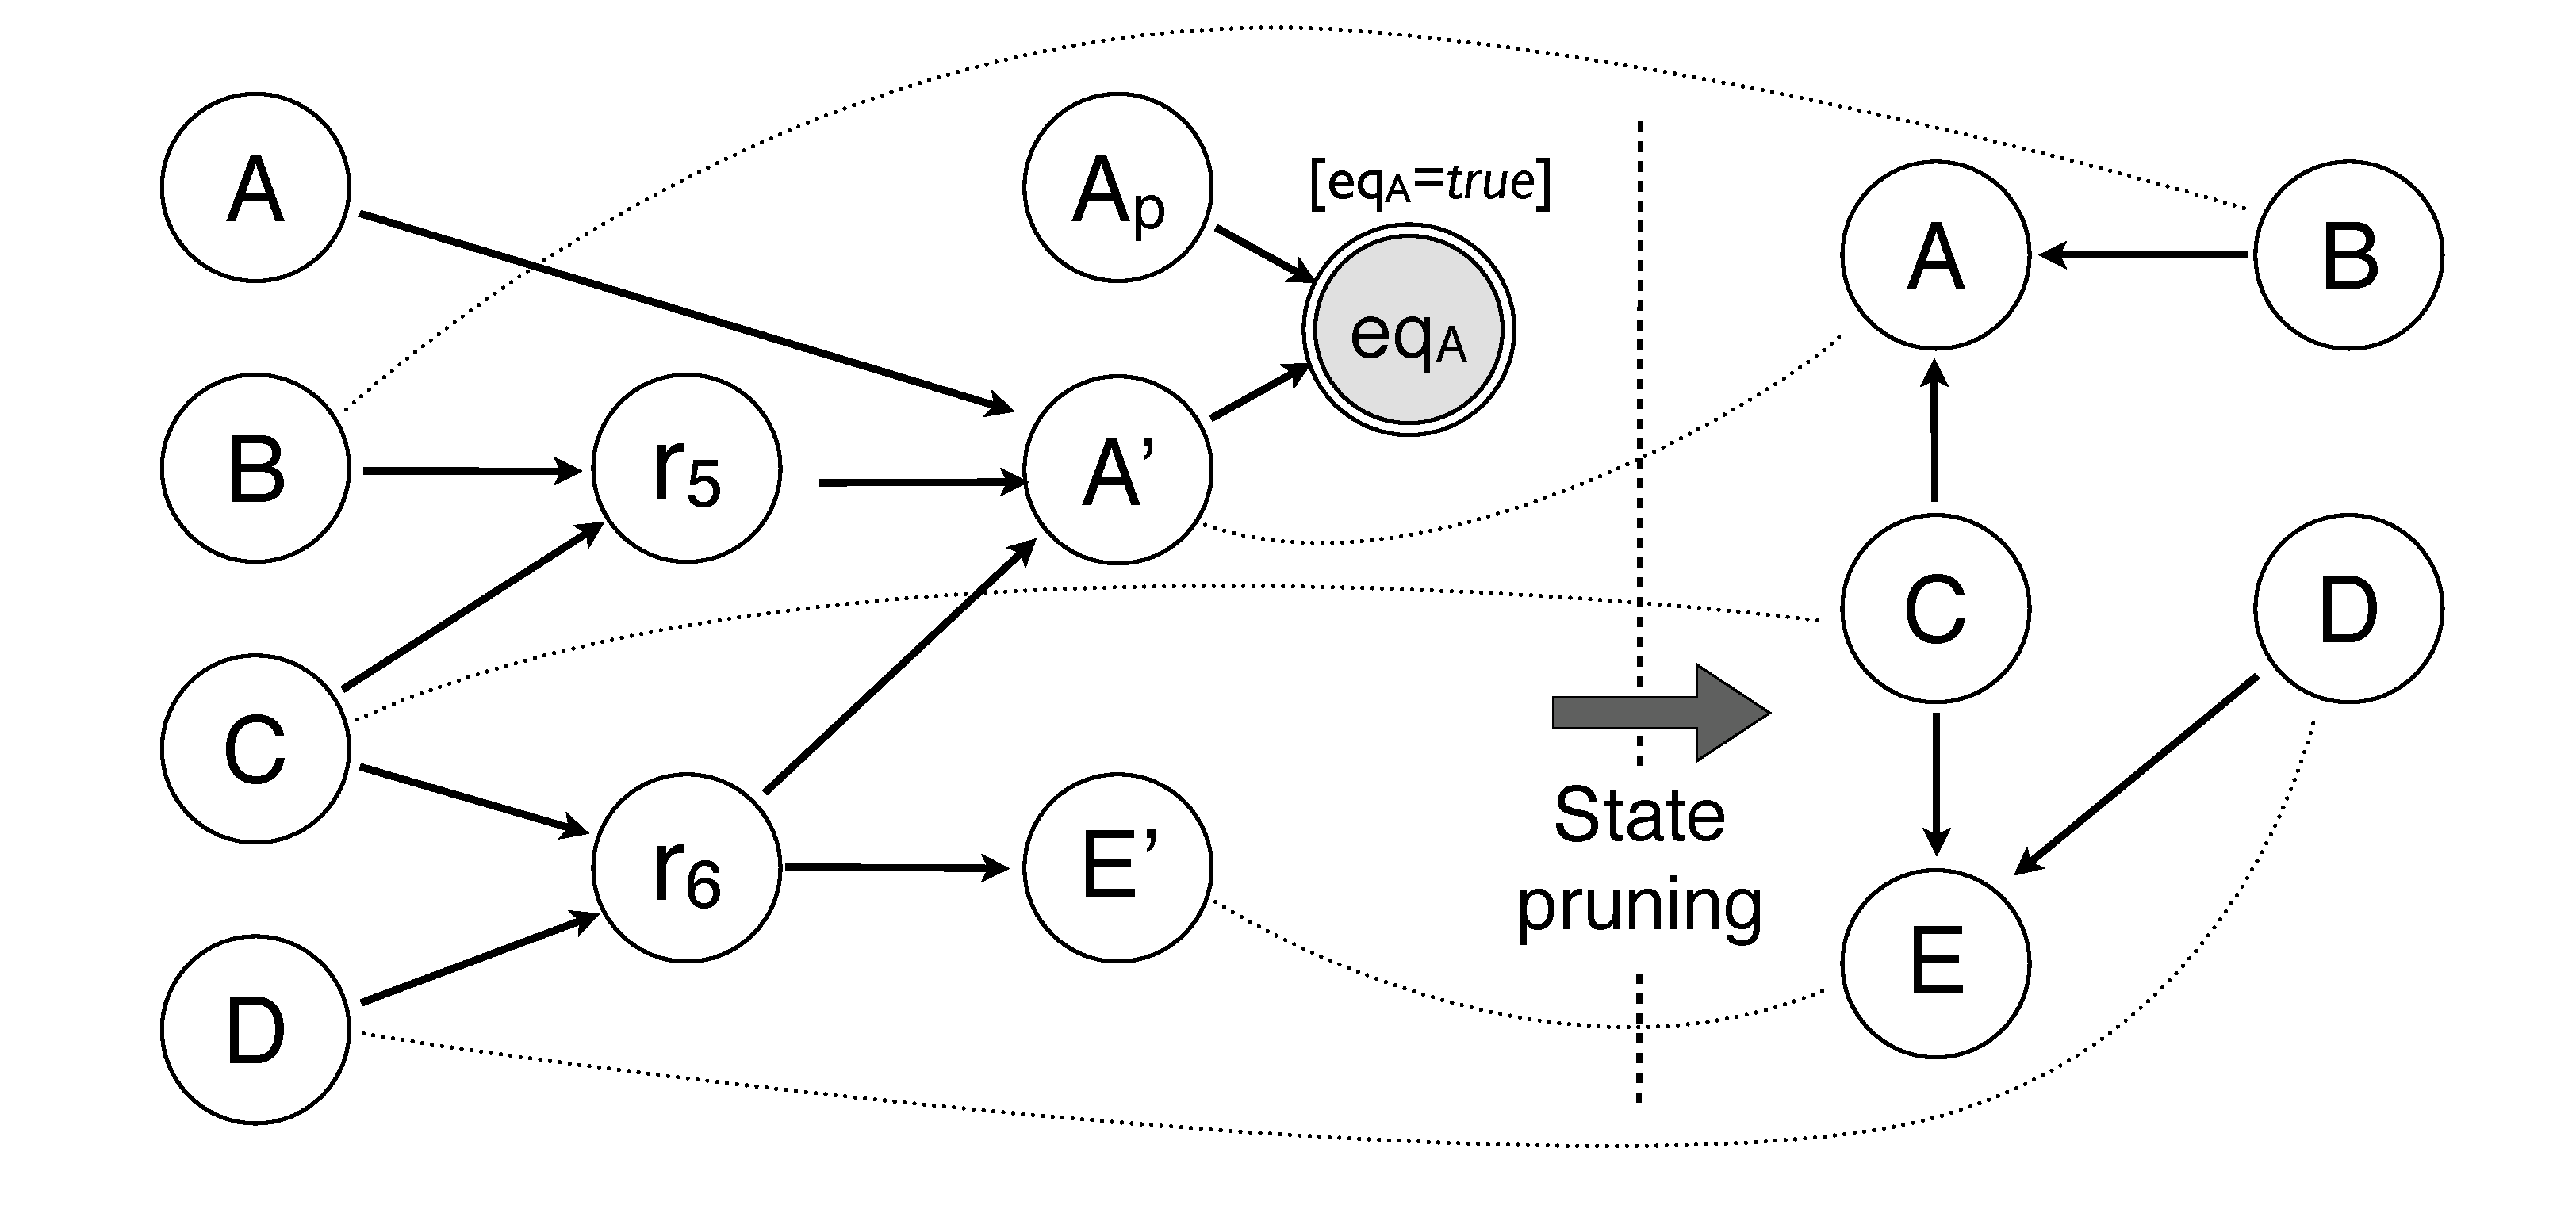
\includegraphics[scale=0.20]{imgs/pruning.pdf}
\caption{Illustration of the state pruning process. Only the nodes $A'$, $B$, $C$, $D$ and $E'$ are retained. The dotted lines denote the correspondence between nodes.}
\label{fig:pruning}
\end{figure}


\subsection{Detailed example}
\label{sec:detailedexample}

We now describe a minimal but complete example of workflow for a short interaction. 

\subsubsection*{Description}

Assume a domain similar to the one shown in Figure \ref{fig:fsa}, where a user can request a robot to move forward, backward, left, right, or stop.  The set of dialogue acts $a_u$ that can be recognised by the system is the following: 
\begin{center}
$\{\mathit{Request(Forward)}$, $\mathit{Request(Backward)}$, $\mathit{Request(Left)}$, \\ $\mathit{Request(Right)}$, $\mathit{Request(Stop)}$, $\mathit{Other}\}$. \\
\end{center}
The corresponding system actions $a_m$ are: 
\begin{center}
$\{\mathit{Move(Forward)}$, $\mathit{Move(Backward)}$, $\mathit{Move(Left)}$, \\ $\mathit{Move(Right)}$, $\mathit{Move(Stop)}$, $\mathit{AskRepeat}\}$. 
\end{center}
The objective of the system is to fulfil the user command if it is reasonably confident regarding which action to execute.  Otherwise, the system asks the user to repeat. 

\subsubsection*{Domain specification}

The domain specification designed for this constructed example is constituted of an empty initial state and the following two rule-based models: \begin{itemize}
% = \langle \langle a_u \rangle, \langle r_9, r_{10} \rangle \rangle$
\item Model $m_1$ is triggered by $a_u$ and includes the two utility rules $r_{9}$ and $r_{10}$:
\begin{align*}
r_{9}: \ \ & \forall y: \\ 
& \textbf{if} \ (a_u = Request(y)) \ \textbf{then} \\ 
& \; \; \begin{cases} 
U(a_m = Move(y)) = 2 \\ 
\end{cases} \\
& \textbf{else} \\ 
& \; \; \begin{cases} 
U(a_m = Move(y)) = -2 \\ 
\end{cases} \\[4mm]
r_{10}: \ \ &  \; \; \begin{cases} U(a_m = \mathit{AskRepeat}) = 0.5 \end{cases}
\end{align*}

Rule $r_{9}$ specifies that the utility of executing the action corresponding to the user command is 2, with a penalty of $-2$ when the wrong action is executed. Rule $r_{10}$ assign a utility of 0.5 for asking a clarification question.\footnote{As the action selection process presented thus far does not perform forward planning, the utilities provided in this example correspond to long-term expected utilities (Q-values in the reinforcement learning terminology).}

%= \langle \langle a_m \rangle, \langle r_{11} \rangle \rangle
\item Model $m_2$ is triggered by $a_m$ and has one single predictive rule $r_{11}$: 
\begin{align*}
r_{11}: \ \ & \forall y: \\ 
& \textbf{if} \ (a_m = \mathit{AskRepeat} \land a_u=y) \ \textbf{then} \\ 
& \; \;  \begin{cases} 
P(a_{u\mbox{-}p} = y) = 0.9 \\ 
\end{cases}
\end{align*}
Rule $r_{11}$ specifies that the probability that the user will repeat his last utterance when asked by the system to do so is expected to be $0.9$.
\end{itemize}

\subsubsection*{Processing workflow}

We now detail the processing workflow associated with the following constructed interaction:
\begin{dialogue} 
\speak{User } Now move forward \\ $\phantom{b}$ $\tilde{a}_u = \langle (\mathit{Request(Forward)}, 0.6), (\mathit{Request(Backward)}), 0.4)\rangle$  \\[-3mm]
\speak{System } Could you please repeat? \\[-3mm]
\speak{User } Please move forward! \\ $\phantom{b}$ $\tilde{a}_u = \langle (\mathit{Request(Forward)}, 0.7), (\mathit{Other}, 0.2), (\mathit{Request(Backward)}, 0.1) \rangle$ \\[-3mm]
\speak{System } OK, moving forward!
\end{dialogue}
The (constructed) recognition hypotheses $\tilde{a}_u$ produced by the ASR/NLU components are written underneath the user utterance. 

Figure \ref{fig:detailedexample} details the steps involved in the state update procedure that follows from the reception of dialogue act hypotheses from the natural language understanding component. 

%Note that the probability and utility distributions shown in the figure are marginalised on their dependent variables.

\begin{figure}[p]
\centering
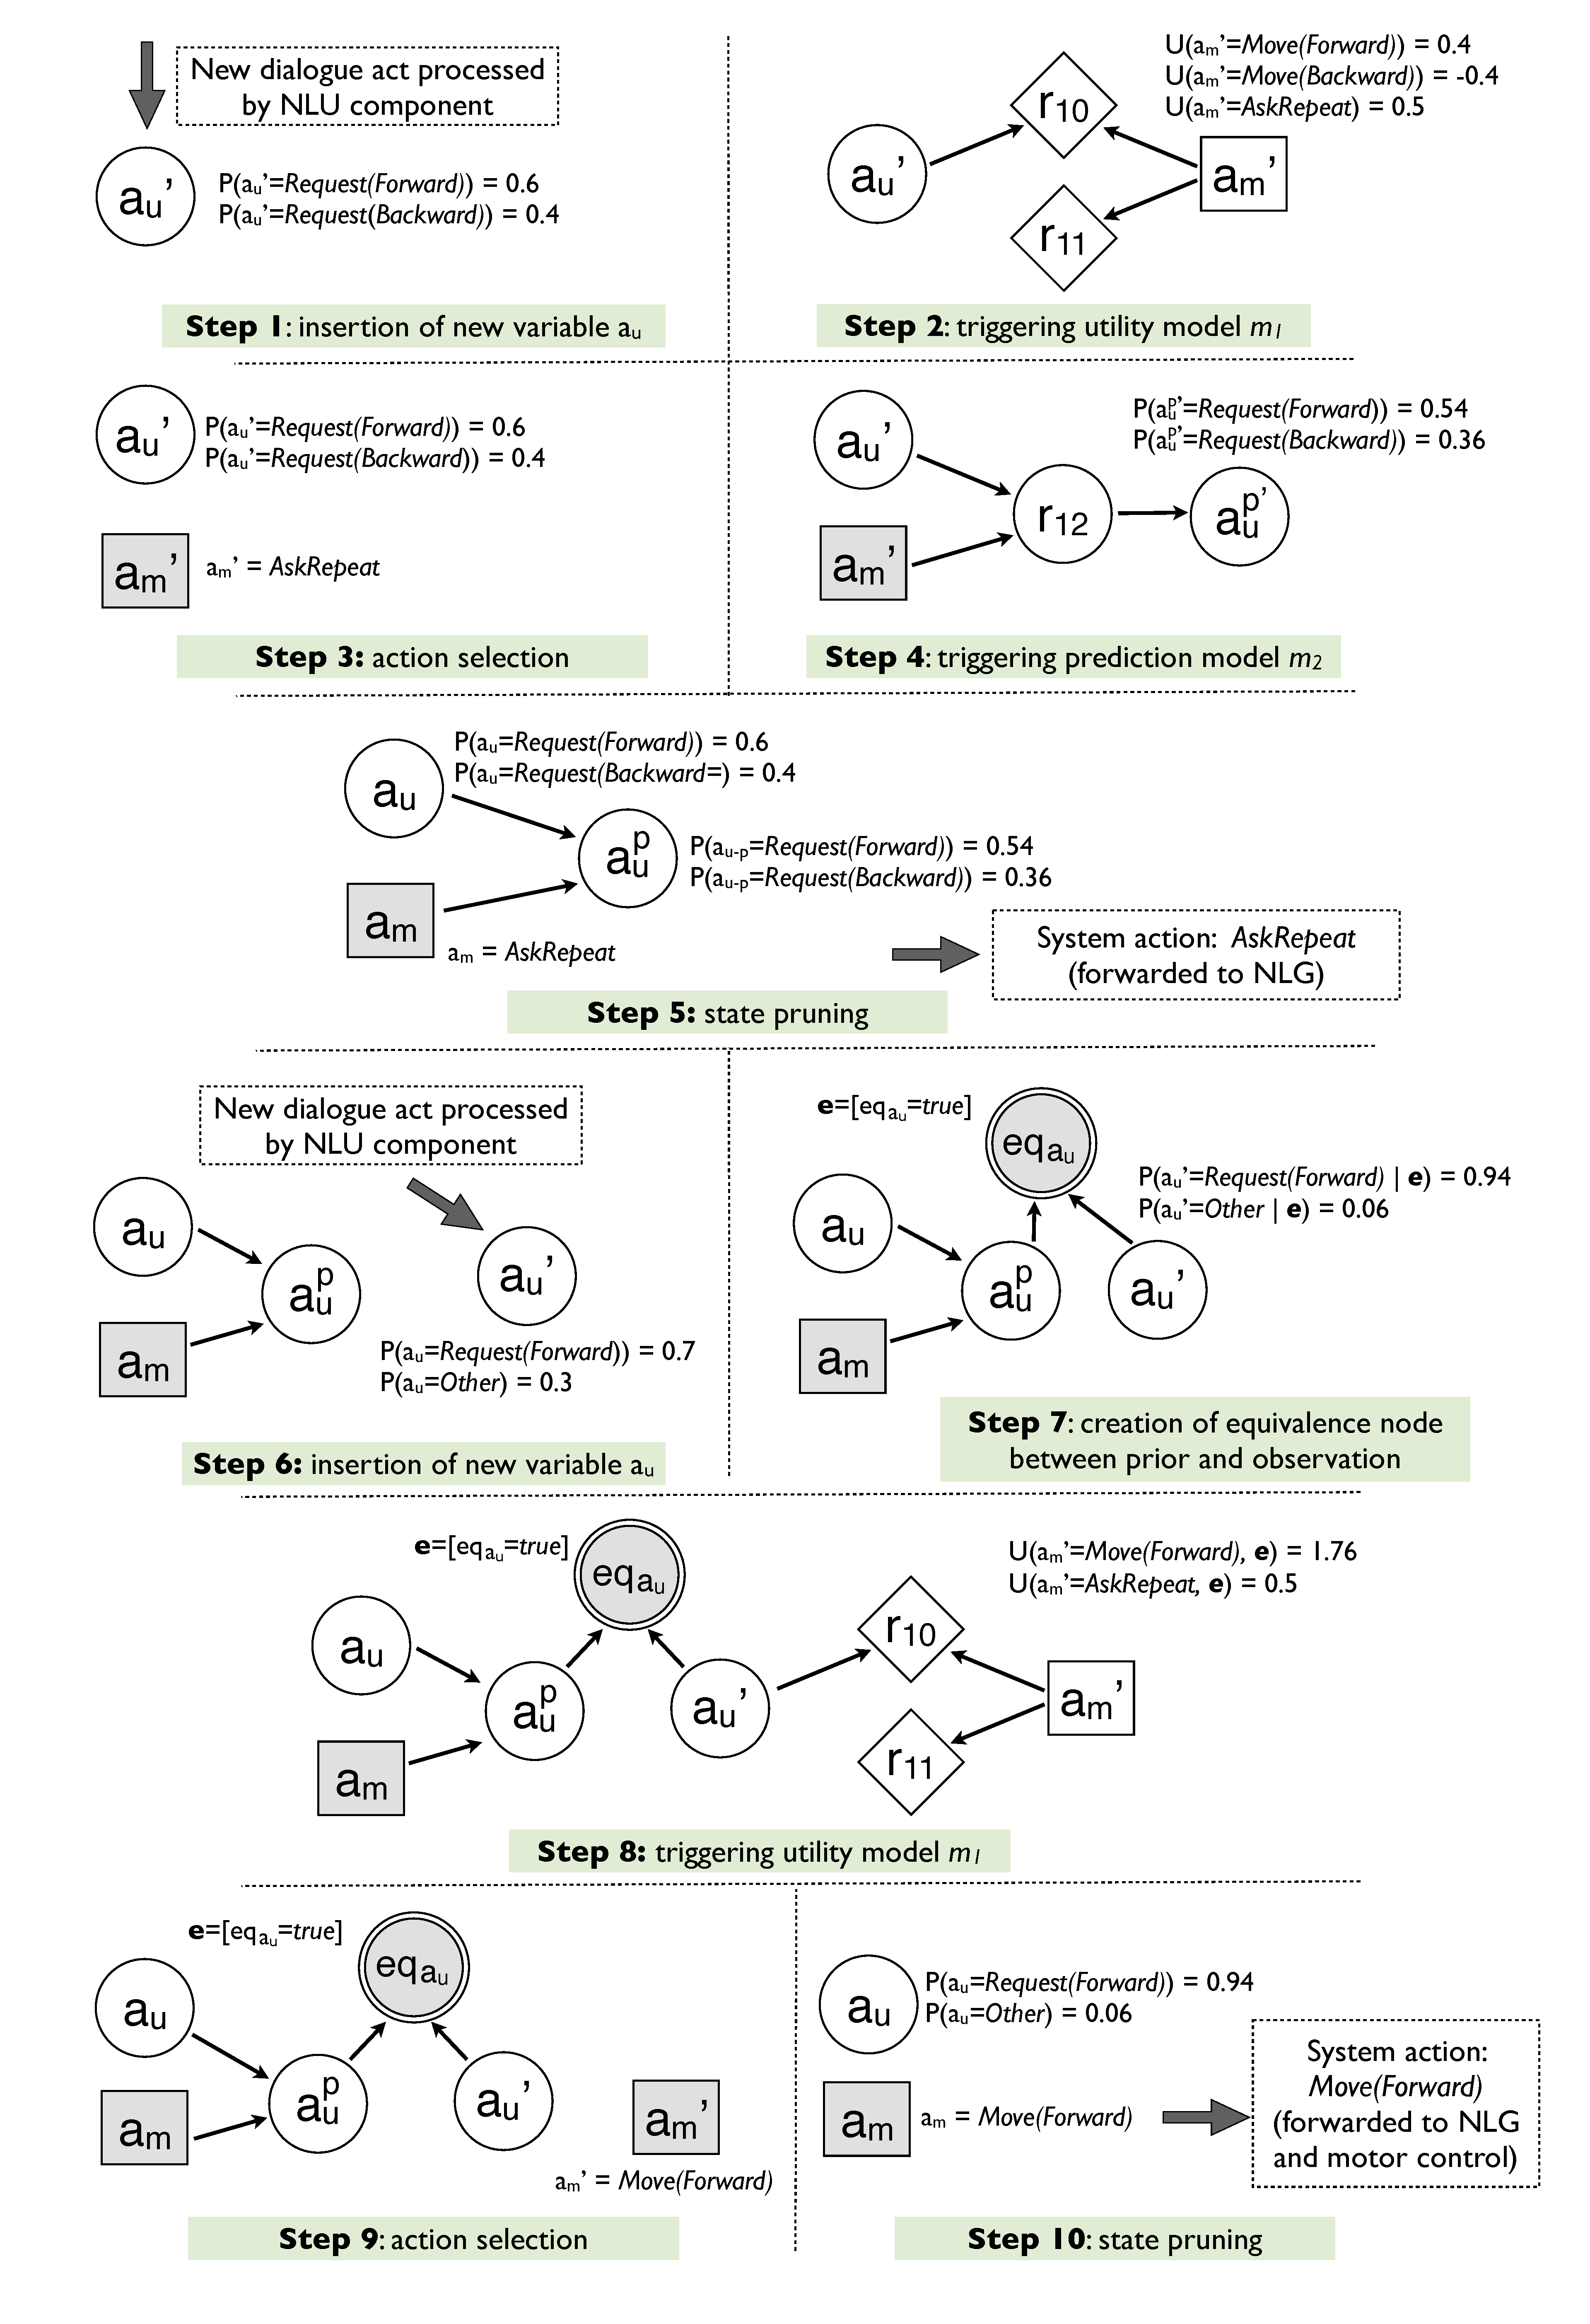
\includegraphics[scale=0.25]{imgs/detailedexample.pdf}
\caption{Detailed example of processing workflow. }
\label{fig:detailedexample}
\end{figure}
 
Step 1 inserts the new dialogue act hypotheses on the dialogue state.  This insertion triggers 
the utility model $m_1$. The instantiation results in Step 2 in the creation of two utility nodes and one decision node.  The optimal action to perform in such case is $\mathit{AskRepeat}$, which is selected by the system in Step 3. The action selection triggers model $m_2$ in Step 4, which creates a prediction node $a_{u\mbox{-}p}'$ expressing the expected probability distribution for the next user dialogue act. The state is finally pruned of the intermediary rule node in Step 5.  System components such as NLG can react on the updated state and generate the proper linguistic realisation of the system action. The system then waits for the user input, which is shown in Step 6.  The relation between the predicted and actual user response leads in Step 7 to the creation of an equivalence node, and the inclusion of the assignment $eq_{a_u} = true$ in the evidence. We notice that the combination of the prior distribution over predicted values and the actual distribution over dialogue act hypotheses increases the probability of $a_u' = \mathit{Request(Forward)}$. Step 8 triggers the model $m_1$ based on the new user input.  The optimal action is this case is $\mathit{Move(Forward)}$, which is selected in Step 9.  This selection triggers model $m_2$, but rule $r_{11}$ only generates in this case an empty effect and is therefore directly deleted. Finally, the state is pruned of its intermediary nodes in Step 10, retaining only the last user and system actions $a_u$ and $a_m$. 

In comparison to the finite-state solution present in Figure \ref{fig:fsa}, we observe that the rule-structured approach defined by models $m_1$ and $m_2$ allows the dialogue manager to 
accumulate evidence over time and prime the recognition hypotheses of the user dialogue act $a_u$ based on the previous dialogue act.  This accumulation of evidence is absent from the FSA, due its rigid state representation and lack of memory. 

\section{Advanced modelling}
\label{sec:amodelling}

Dialogue domains often include random variables with values expressed via specific data structures such as lists or strings. The rule-based formalism described in the previous sections can be easily complemented with special-purpose tools to efficiently operate on these data structures. We first explain how conditions and effects can be defined on variables that represent lists, and then discuss how rules can manipulate strings. 

\subsection{Operations on lists}

Some state variables are best represented as lists of elements. For instance, the dialogue state may include random variables that enumerate  the $n$ most recent dialogue acts in the interaction history, the stack of tasks that remain to perform, or the list of visual objects perceived by the system.  The range of values for such state variables is the power set of its possible elements. 


Special-purpose operators for the manipulation of such lists can be integrated in both the conditions and effects of probabilistic rules: 
\begin{itemize}
\item Rule conditions can include operators to check the presence or absence of particular elements in a list, such as $a \in A$ or $a \notin A$. 
\item Rule effects can also be augmented to manipulate elements from a list.  Three new types of effects are created to this end, in addition to the traditional assignment of output values: \textit{add effects} (adding an element to a list), \textit{delete effects} (deleting an element from a list) and \textit{clear effects} (clearing all elements of a list). The resulting lists are sorted by insertion order. 
\end{itemize}

Figure \ref{fig:seteffects} illustrates two rules that apply these new effects to update a state variable $A$. 
 
\begin{figure}[h]
\centering
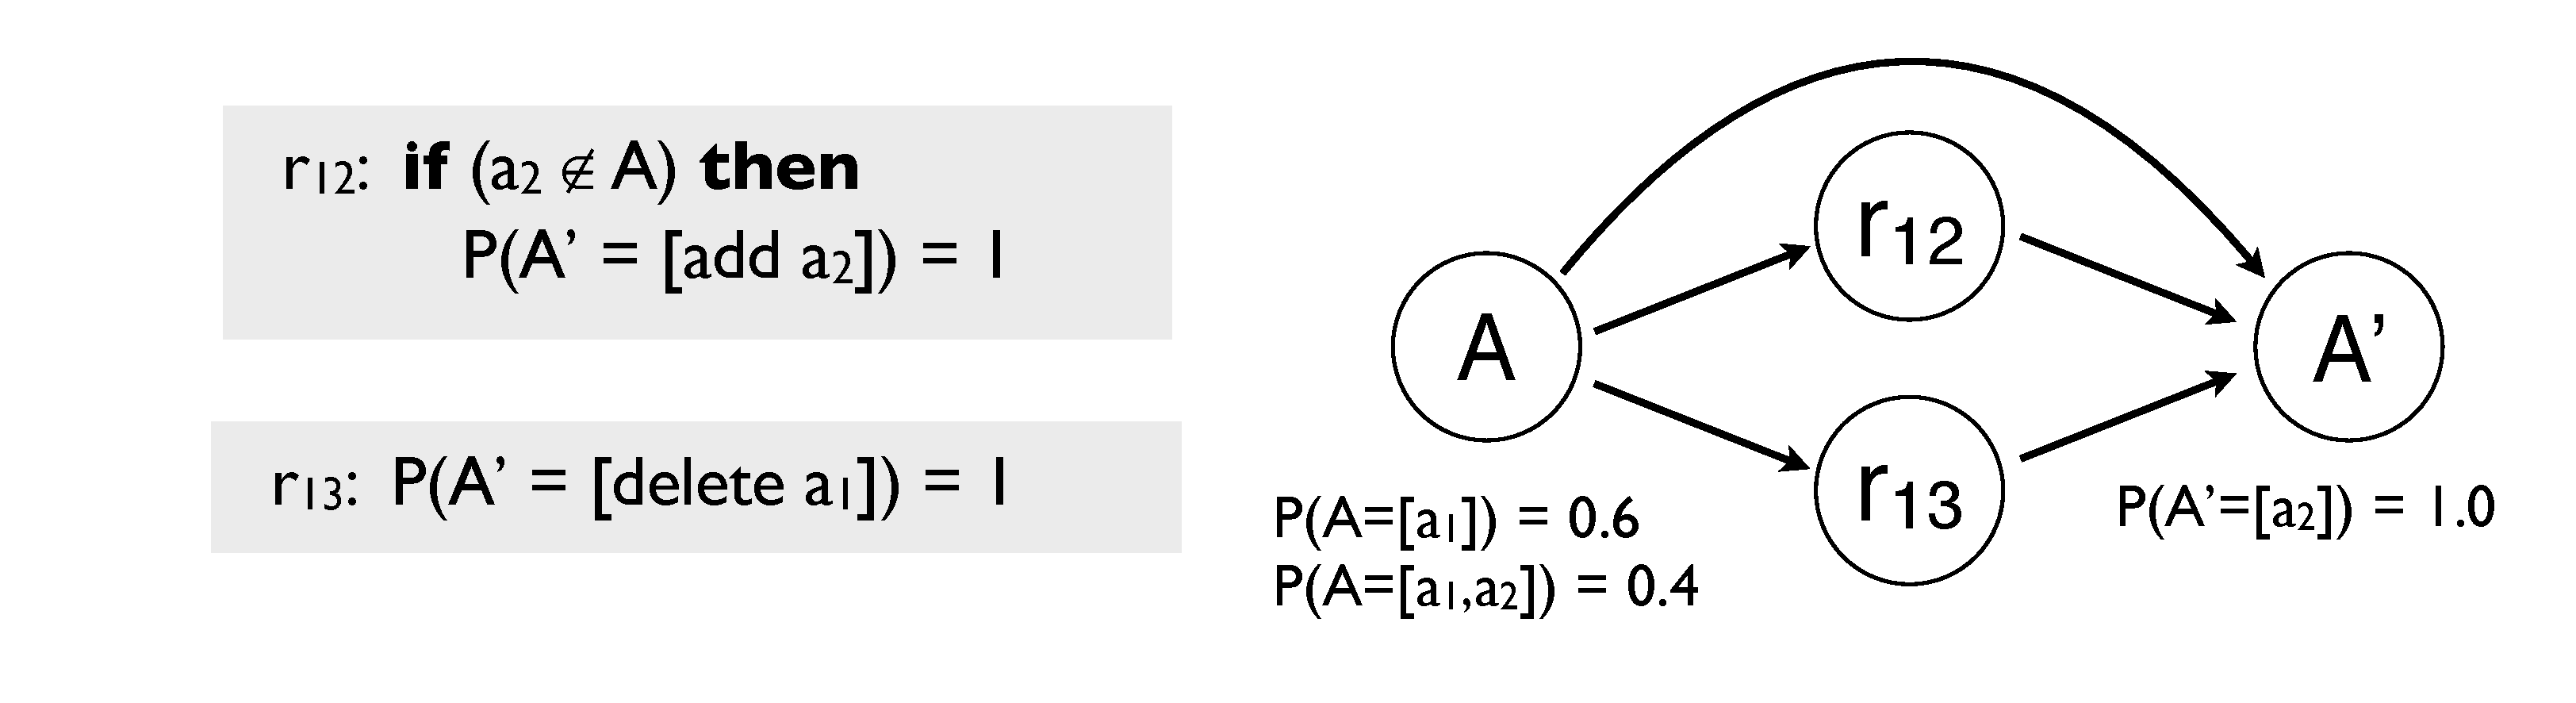
\includegraphics[scale=0.25]{imgs/seteffects.pdf}
\caption{Example of rules using add/delete effects to manipulate lists.}
\label{fig:seteffects}
\end{figure}

These new effects can be incorporated to the framework through a simple modification of the output distribution. Let $\mathbf{e}$ denote as before the conjunction of all effects $e_1 \land ... e_n$. In addition to the previously defined set of values $\mathbf{e}(X)$ assigned for the variable $X$, we construct two new sets of values $\mathbf{e}_{add}(X)$ and $\mathbf{e}_{del}(X)$ that represent the values that are respectively added and deleted for the variable $X$ through the new effects we just described. Note that $\mathbf{e}_{del}(X)$ may include all values for $X$ if the clear effect is applied. 

The output distribution in Equation \eqref{eq:outputdist2} is then rewritten as:
\begin{align}
&P(X'\!=\!x' \, | \, r_1\!=\!e_1,... r_n\!=\!e_n, X\!=\!x) = \hspace{5cm} \nonumber \\ & \; \; \; \; \; \; \; \; \; \;  \begin{dcases} 
\frac{\sum_{v \in {\mathbf{e}(X)}} \mathbf{1}(x' = v)} { |\mathbf{e}(X)| }  & \text{if } \mathbf{e}(X)\!\neq\!\emptyset \\
\mathbf{1}(x' = \left(\mathbf{e}_{add}(X) \cup \left(x \; / \; \mathbf{e}_{del}(X)\right)\right)) & \text{otherwise} \\
\end{dcases}\label{eq:outputdist4}
\end{align} 

The output distribution associated for a new variable (cf. Equation \eqref{eq:outputdist1}) can be rewritten in a similar manner.

%The assignment effects in $\mathbf{e}(X)$ and the add/delete effects in $\mathbf{e}_{add}(X)$ and $\mathbf{e}_{delete}(X)$ being mutually incompatible, the assignment effects are assumed to take precedence.

%Lists are defined to be equal if they include the same elements in the same order.

%Other types of collections such as sets with no duplicate elements can be exploited in the same manner. 

\subsection{Operations on strings}

Many of the data structures present in the dialogue state are strings -- the most prominent ones being the last user utterance $u_u$ and the last system utterance $u_m$. The integration of special-purpose functionalities for manipulating strings within the conditions and effects of probabilistic rules is therefore desirable. In particular, rules can be extended to perform template-based string matching operations.  The idea is to include a new type of conditions that checks whether a string matches a given template.  Both full and partial matching can be employed. Templates are allowed to include slots to fill. These slots are conceptually similar to the quantified variables discussed in Sections \ref{sec:quantification} and \ref{sec:applicationquantif}. A successful match will thus generate values for the filled slots, which will be included as part of the groundings for the rule. 

Figure \ref{fig:stringmanip} illustrate how such rules are applied in practice.  $\{OBJ\}$ denotes a slot that is to be filled through matching the template with the value specified in $u_u$. 
\begin{figure}[h]
\centering
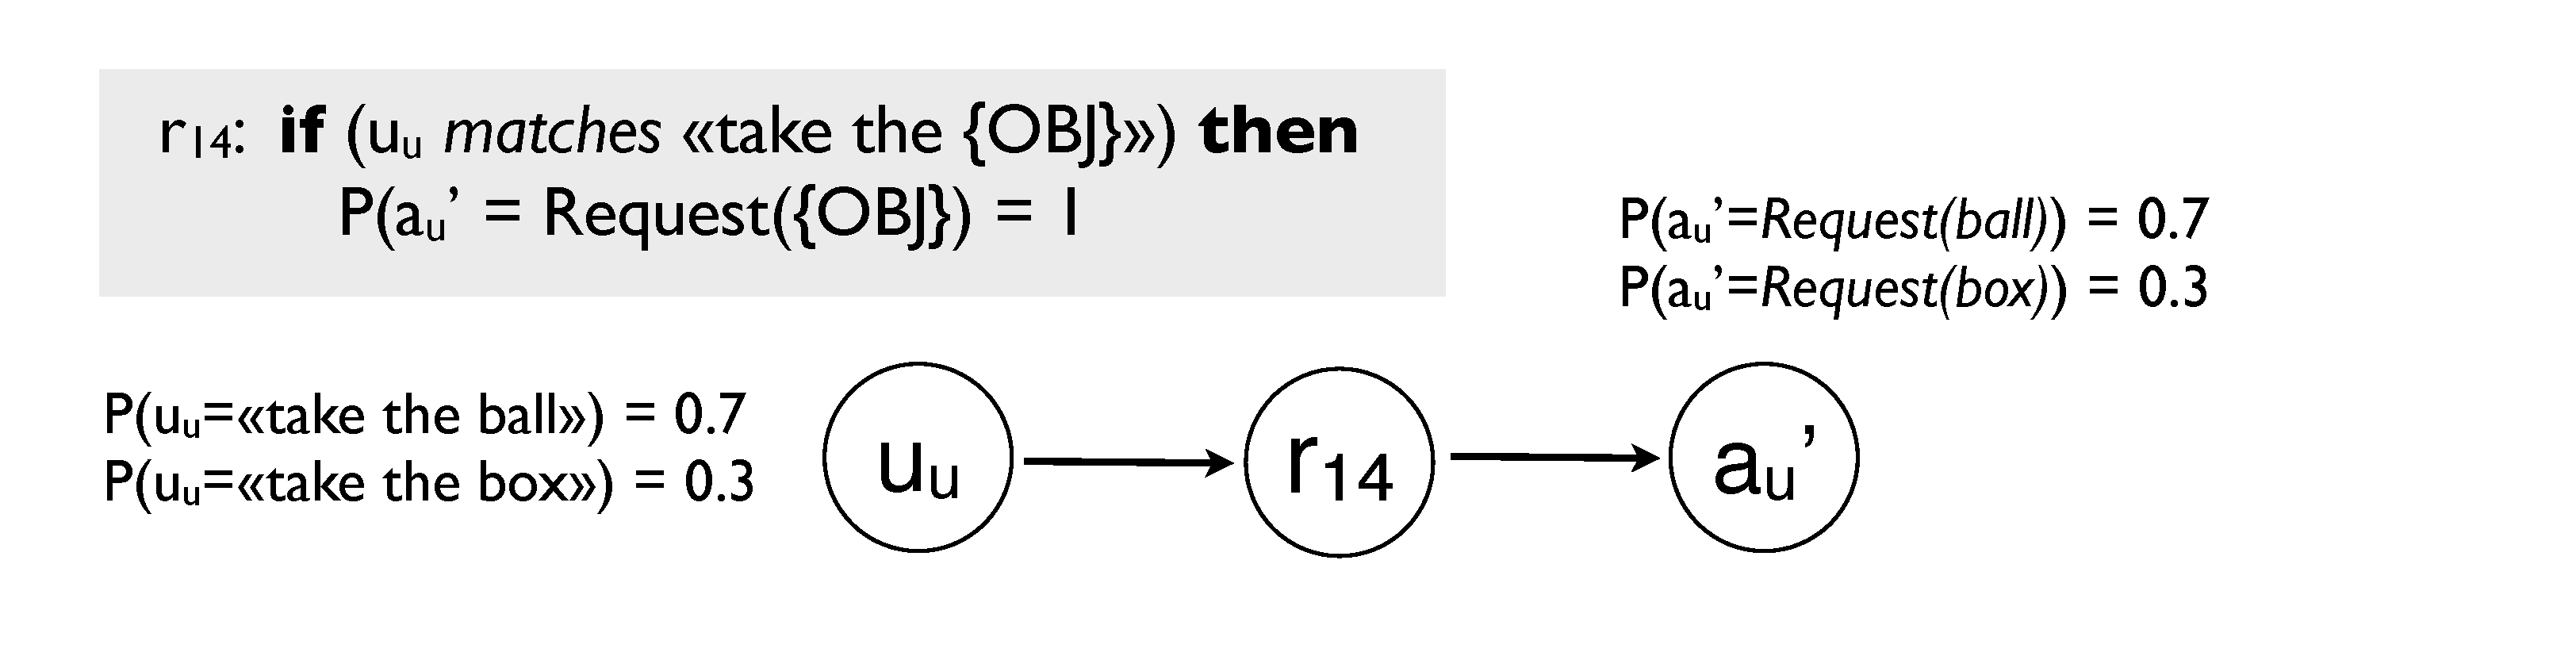
\includegraphics[scale=0.25]{imgs/stringmanip.pdf}
\caption{Example of rule using string matching operations.}
\label{fig:stringmanip}
\end{figure}

\section{Relation to previous work}
\label{sec:relatedwork}

The idea of using structural knowledge in probabilistic models has been explored in many directions, both in the fields of decision-theoretic planning and reinforcement learning \citep{Hauskrecht98,Pineau2004,KerstingR04,lang10jair,Otterlo2012} and in statistical relational learning \citep{Jaeger01,Richardson:2006,getoor:srlbook07}.  The introduced structure may be hierarchical, relational, or both. As in our approach, most of these frameworks rely on the use of expressive representations serving as templates for the generation of classical probabilistic models.  The surveys of \cite{Otterlo2006,Otterlo2012} provide a complete overview of relational and first-order logical approaches for reinforcement learning in Markov decision processes, covering both model-free and model-based methods.  While the formalisation presented in this thesis and the aforementioned approaches share many insights, they also reveal several interesting differences: 

\begin{itemize}

\item Probabilistic rules are primarily tailored for dialogue management tasks and seek to capture dialogue domains by striking a balance between propositional and first-order logic. The formalism deliberately eschews the complexity of full-scale first-order probabilistic inference to ensure that the domains models can be applied under real-time constraints. This design choice sets it apart from other frameworks such as Markov Logic Networks which can express arbitrary first-order formulae but are often tedious to instantiate due to the size and complexity of the resulting models.\footnote{See however \cite{Kennington:2012} for an approach that attempts to apply Markov Logic Networks to natural language understanding tasks.} 

\item Probabilistic rules are also designed to operate under partially observable settings, as state uncertainty is a pervasive and unavoidable aspect of verbal interactions.  By contrast, most previous work on relational probabilistic models are limited to fully observable environments, with the exception of some limited theoretical studies by \cite{Wang:2010,SannerK10}. 

\item Finally, the presented framework posits that the \textit{if ... then ... else} structures of probabilistic rules are best encoded by the system designers based on their expert knowledge of the domain, while the rule parameters can be estimated empirically. We therefore exclude the problem of structure learning from the scope of this thesis, as opposed to several approaches in which the domain rules and constraints are extracted via machine learning techniques \citep{PasulaZK07,Kok:2009}.

\end{itemize}

Probabilistic rules also bear similarities with planning description languages such as the Planning Domain Description Language \citep[PDDL, see ][]{mcdermott1998} and its probabilistic extension, the Probabilistic Problem Description Language \citep[PPDDL, see ][]{younes2004ppddl1}.  These languages are structured through action schemas that specify how (parametrised) actions can yield particular effects under various conditions. As in probabilistic rules, these languages try to carefully balance between the language expressivity and the complexity of the planning algorithm, based on a subset of first-order logic. A relational extension of PDDL, named RDDL, has also been introduced in recent planning competitions \citep{Sanner:RDDL}. The learning techniques presented by \cite{PasulaZK07} to estimate transition functions based on noisy indeterministic deictic rules is directly related to our approach, as is the recent work \cite{lang10jair} on probabilistic noisy planning rules.   Both frameworks define conditions associated with probabilistic distributions over effects. Their approaches are however restricted to fully observable settings. 

In the dialogue management literature, most structural approaches rely on a clear-cut task decomposition into goals and sub-goals \citep{Allen:2000:AGD:973935.973937,Steedman-Petrick:07,Bohus:2009}, where the completion of each goal is assumed to be fully observable, discarding any remaining uncertainty.  Our own work on multi-policy dialogue management in \cite{multipolicy-sigdial2011} relaxes the assumption of perfect knowledge of task completion, handling multiple policies as a problem of probabilistic inference over activation variables.  Probabilistic rules can be considered an extension of this early work, where the structural knowledge is not confined to task decomposition but is extended to generic rules over state variables.  

The formalism presented in this chapter is strongly inspired by information-state approaches to dialogue management \citep{Larsson:2000,Bos2003}, which are also based on a shared state representation that is updated according to a rich repository of rules.  \cite{Ginzburg2012} also models conversational phenomena by way of update operations that are encoded with rules mapping conditions to effects. However, contrary to the framework presented here, the rules specified in these approaches are generally deterministic and do not include learnable parameters. The action selection mechanism is also conceptualised slightly differently, as information-state frameworks rely on rules that directly select the most appropriate action given the current state. Probabilistic rules adopt by contrast a decision-theoretic approach that divides action selection in two stages: rules first provide utility distributions for the system action, and the system then searches for the action that yields the maximum expected utility. 

The literature on dialogue policy optimisation with reinforcement learning also contains several approaches dedicated to dimensionality reduction for large state-action spaces, such as function approximation \citep{Henderson:2008}, hierarchical reinforcement learning \citep{Cuayahuitl:2010} and summary POMDPs \citep{Young:2010}.  Many of these techniques have already been discussed in Section \ref{sec:application-dm} and will therefore not be repeated here. Most current approaches in dialogue policy optimisation focus on large but weakly structured state spaces (generally encoded as large lists of features), which are suited for slot-filling dialogue applications but are difficult to transfer to more open-ended or relational domains.  The idea of state space partitioning, implemented here via high-level conditions, has also been explored in recent papers \citep[see e.g. ][]{Williams2010}. \cite{Crook:2010} explored the introduction of complex user goal states including disjunction and negation operators. \cite{Heriberto2011} describes a policy optimisation approach based on logic-based representations of the state-action space for relational MDPs. The main difference with our approach lies in his reduction of the belief state to fully observable variables whereas we retain the partial observability associated with each variable.  The work of \cite{Mehta:2010,Raux2011} demonstrated how tree-structured Bayesian networks called probabilistic ontology trees can improve belief tracking performance.  The tree structure is derived in their work from a hierarchical concept structure .  Finally, \cite{neill2011} describe a procedure for dialogue strategy selection based on probabilistic logic.

\section{Conclusion}

This chapter presented the formalism of probabilistic rules, which forms the core of the modelling approach developed in this thesis. We started by arguing that dialogue models are often highly structured, and that this structure can be leveraged by (1) introducing latent variables, (2) partitioning value assignments for the parent variables, and (3) making use of quantification. We then explained how these structural insights can be transferred into a new framework -- probabilistic rules -- that combines concepts borrowed from both first-order logic and probability theory in order to get ``the best of both worlds'', i.e. a representation formalism that is both richly expressive and capable of capturing uncertain knowledge.  These rules are practically defined as \textit{if...then...else} control structures that associate high-level conditions on input variables to probabilistic effects on output variables.  Multiple extensions of the formalism have been developed to e.g. encode utility distributions, enclose universal quantifiers, and efficiently manipulate data structures such as lists and templates. 

At runtime, these rules are instantiated in the Bayesian network representing the current dialogue state. The instantiation procedure creates a latent node for each rule, which is conditionally dependent on the input variables of the rule.  For probability rules, this node is a chance node that expresses a probability distribution over the possible effects of the rule. Utility rules are similarly instantiated with a utility node expressing the utility distribution for specific decision variables.  Universally quantified variables can be included in the conditions and effects of the rules, allowing particular aspects of the rule to be underspecified. The rules are grouped into models that are attached to the dialogue state and are triggered upon relevant state updates. 

Probability and utility rules effectively function as high-level templates for the definition of a dynamic decision network. The expressive power of these rules allows them to efficiently encode complex relations between variables, and thereby reduce the number of parameters to estimate.  We have however not yet detailed how this parameter estimation is practically performed. The next two chapters provide answers to this important question. 



\chapter{Learning from Wizard-of-Oz data}
\label{chap:wozlearning}

The previous chapter presented the formalism of probabilistic rules and described their practical instantiation as latent nodes of a graphical model. Probabilistic rules are generally associated to a number of parameters, which may either express probabilities over effects (for probability rules) or utilities associated with particular decisions (for utility rules). But where exactly do these probabilities and utilities come from?
\index{supervised learning}
This thesis develops two distinct approaches to this question. The present chapter concentrates on the first approach, which is grounded in supervised learning techniques. We demonstrate how rule parameters can be optimised to best imitate the action choices of a human expert through a process of statistical estimation based on Wizard-of-Oz data. The next chapter will then detail an alternative reinforcement learning approach to the same task.

The chapter is divided in three sections.  Section \ref{sec:rule-params} describes how uncertainty regarding the value of rule parameters can be explicitly represented through prior distributions. Section \ref{sec:rule-supervised} goes on to explain how these distributions can be gradually refined through Bayesian learning on data gathered from Wizard-of-Oz interactions.  The learning algorithm  is used to progressively narrow down the spread of the parameter distributions to the values providing the best fit for the training data. Finally, Section \ref{sec:wozlearning-experiments} reports on experimental results in a human--robot interaction domain for which small amounts of Wizard-of-Oz data were recorded. The experiment compared the learning performance of a utility model structured with probabilistic rules against two baselines respectively encoded with plain utility tables and with linear models. The evaluation showed that the rule-structured model was able to imitate the dialogue policy followed by the wizard significantly better than its unstructured counterparts.

\section{Parameters of probabilistic rules}
\label{sec:rule-params}

\subsection{General methodology}

The examples of probabilistic rules seen so far all relied on fixed probability and utility values. These values can, however, be replaced by parameters that reflect unknown values that are to be estimated empirically, on the basis of training data. 
 
The overall structure of parametrised rules remains essentially identical to the one outlined in the previous chapter.  Probability rules are once more defined in terms of conditions $c_i$ associated to probability distributions $P(E_i)$ over effects.  The probability of each effect $e_{(i,j)}$ is, however, no longer fixed but is instead represented by a parameter $\theta_{(i,j)}$, giving rise to the following skeleton: 
\begin{equation}
\begin{aligned}
& \textbf{if} \ \ (c_{1}) \ \ \textbf{then} \\ 
& \;\;\;\;\; \begin{cases}
P(E_1\!=\!e_{(1,1)}) = \theta_{(1,1)} \\
 \dots \\
P(E_1\!=\!e_{(1,m_1)}) = \theta_{(1,m_1)} 
\end{cases} \\[3mm]
%& \textbf{else if} \ \ (c_{2}) \ \ \textbf{then} \\ 
%& \;\;\;\;\; \begin{cases}
%P(E_2\!=\!e_{(2,1)}) = \theta_{(2,1)}, \\
% \dots \\
%P(E_2\!=\!e_{(2,m_2)}) = \theta_{(2,m_2)}
%\end{cases} \\ 
& \dots  \\
& \textbf{else} \\
& \;\;\;\;\; \begin{cases}
P(E_{n}\!=\!e_{(n,1)}) = \theta_{(n,1)} \\
\dots \\
P(E_{n}\!=\!e_{(n,m_n)}) = \theta_{(n,m_n)}
\end{cases}
\end{aligned}
\end{equation}

Parametrised utility rules analogously replace utility values with unknown parameters:
\begin{equation}
\begin{aligned}
& \textbf{if} \ \ (c_{1}) \ \ \textbf{then} \\ 
& \;\;\;\;\; \begin{cases}
U_1(d_{(1,1)}) = \theta_{(1,1)} \\
 \dots \\
U_1(d_{(1,m_1)}) = \theta_{(1,m_1)}
\end{cases} \\[3mm]
%& \textbf{else if} \ \ (c_{2}) \ \ \textbf{then} \\ 
%& \;\;\;\;\; \begin{cases}
%U_2(d_{(2,1)}) = \theta_{(2,1)} \\
% \dots \\
%U_2(d_{(2,m_2)}) = \theta_{(2,m_2)}
%\end{cases} \\
& \dots  \\
& \textbf{else} \\
& \;\;\;\;\; \begin{cases}
U_n(d_n^1) = \theta_{(n,1)} \\
\dots \\
U_n(d_{(n,m_n)}) = \theta_{(n,m_n)}
\end{cases}
\end{aligned}
\end{equation} 

We focus in this work on the problem of parameter estimation given a known and fixed rule structure.  The methodological stance adopted in this thesis rests on the idea that the structure of probabilistic rules is best defined by the system designer, while the rule parameters is best determined by statistical optimisation techniques. Based on our own practical experience with various dialogue systems, we believe that such a division of labour between the human designer and the learning algorithm is a sensible one, as system designers generally have a good grasp of the domain structure and relations between variables but are often unable to quantify the precise probability of an effect or utility of an action.\footnote{Humans are indeed notoriously poor at estimating probabilities and are prone to multiple cognitive biases when doing so, as evidenced by numerous studies in behavioural psychology.  The interested reader is invited to consult e.g.\ \cite{ohagan2006} for more details on the psychological aspects of the human perception of uncertainty and the difficult problem of probability elicitation from experts.}\index{probability distribution!elicitation of}

Although our work concentrates on parameter estimation \index{parameter estimation} with a known rule structure, it should be noted that recent developments in statistical relational learning have shown that the structure of stochastic rules can also be extracted from data \citep{PasulaZK07,Kok:2009}  These methods are, however, generally confined to domains of limited size and full observability and are therefore difficult to apply to the types of dialogue domains investigated in this thesis work.  \index{statistical relational learning}


%Domain models can be composed of both fixed and parametrised rules and can therefore accommodate a wide spectrum of learning tasks from fully statistical models with virtually no prior knowledge to manually designed models with only a handful of parameters. 

\subsection{Parameter priors}
\label{sec:rule-params-priors}
\index{rule parameters!Bayesian learning of}
\index{rule parameters!prior distributions of}

Throughout this thesis, we follow a \textit{Bayesian} approach to parameter estimation and associate the rule parameters with explicit prior distributions over their range of possible values.  These prior parameter distributions have a continuous range of values and can be either univariate or multivariate.  The benefits of Bayesian approaches compared to maximum likelihood methods are multiple:
\begin{enumerate} 
\item Bayesian methods allow domain knowledge to be directly included into the learning cycle through the use of informative priors (cf. discussion below). The system designers are thus able to bias the initial prior distributions according to their domain expertise.
\item Bayesian methods explicitly capture the model uncertainty both at the beginning and at the end of the learning process. The outputs of a Bayesian learning cycle are indeed full posterior distributions over the possible parameter values instead of being reduced to point estimates (as for maximum likelihood estimation).  The dialogue agent can therefore explicitly account for parameter uncertainty at runtime and use it to simultaneously learn, reason and act in its environment \citep{Ross:2011}. Furthermore, the reliance on full parameter distributions facilitates the combination of multiple learning processes, as the posterior distribution generated by one learner can be passed on as the prior distribution of another. 
\end{enumerate}

We describe below possible parameter distributions for probability rules and then discuss the case of utility rules.  

\subsubsection*{Probability parameters}
\index{rule parameters!of probability rules}

The distributions over the effects of probability rules are categorical probability distributions.  As already discussed in Section \ref{sec:learning}, the parameter priors of categorical and multinomial distributions are best expressed using \textit{Dirichlet} distributions. \index{Dirichlet distribution}

Each distribution over effects $P(E_i)$ is associated with its own Dirichlet distribution of dimension $m_i$, where $m_i$ is the number of alternative effects (including the empty effect if appropriate).  Rule $r_{1}$ provides an example of a parametrised probability rule: 
\begin{align*}
r_{1}: \ \ \ \ \ & \textbf{if} \ (\mathit{Rain}\!=\!\mathit{false} \land \mathit{Weather}\!=\!\mathit{hot}) \ \textbf{then} \\
& \;\;\;\;\;  \begin{cases}
 P(\mathit{Fire}'\!=\!\mathit{true}) = \theta_{r_{1}(1,1)} \\ 
P(\mathit{Fire}'\!=\!\mathit{false}) = \theta_{r_{1}(1,2)}
\end{cases}  \\ 
& \textbf{else} \\
& \;\;\;\;\; \begin{cases}
P(\mathit{Fire}'\!=\!\mathit{true}) = \theta_{r_{1}(2,1)} \\
P(\mathit{Fire}'\!=\!\mathit{false}) = \theta_{r_{1}(2,2)}
\end{cases} 
\end{align*}


The parameters of rule $r_{1}$ can be expressed with two Dirichlets $\boldsymbol\theta_{r_{1}(1)} = \langle \theta_{r_{1}(1,1)},\theta_{r_{1}(1,2)} \rangle$ and $\boldsymbol\theta_{r_{1}(2)} = \langle \theta_{r_{1}(2,1)}, \theta_{r_{1}(2,2)} \rangle$ respectively associated with the effect distributions for the first and second condition.  The Dirichlet distributions in this example have two dimensions (since two alternative effects are mentioned in the rule), which make them equivalent to \textit{Beta} distributions. 

Dirichlet distributions are continuous, multivariate probability distributions defined by the meta-parameters $\boldsymbol\alpha = [\alpha_1, \dots, \alpha_k]$, where $k$ corresponds to the dimensionality of the categorical distribution of interest.  Dirichlet distributions over the parameters $\theta_1, \dots, \theta_k$ are formally expressed by the following probability density function:
\begin{align}
P(\theta_1, \dots, \theta_k\,; \boldsymbol\alpha) = \frac{1}{\mathrm{B}(\boldsymbol\alpha)} \prod_{i=1}^k \theta_i^{\alpha_i - 1} \ \ \ \text{with } \mathrm{B}(\boldsymbol\alpha) = \frac{\prod_{i=1}^k \Gamma(\alpha_i)}{\Gamma\bigl(\sum_{i=1}^k \alpha_i\bigr)}
\end{align}

where $ \mathrm{B}(\boldsymbol\alpha)$ serves as normalisation factor and builds upon on the gamma function $\Gamma$.\footnote{The gamma function is a generalisation of the factorial for real numbers, and is defined as $\Gamma(z) = \int_0^\infty  t^{z-1} e^{-t}\,{\rm d}t$.} The notation $P(\theta_1, \dots, \theta_k\,; \boldsymbol\alpha)$ refers to the joint density function of the random variables $\theta_1, \dots, \theta_k$ given the specified (hyper-)parameters $\boldsymbol\alpha$. 

Figure \ref{fig:dirichletfun} depicts the shape of the probability density functions for several variants of the two-dimensional Dirichlet distribution $P(\theta_1,\theta_2\,; \boldsymbol\alpha)$.  The second dimension $\theta_2$ is not explicitly shown on the figure but can be directly derived from the first dimension, since $\theta_1 + \theta_2=1$.  The figure illustrates how the $\boldsymbol\alpha$ hyper-parameters determine the shape of the distribution. As the $\boldsymbol\alpha$ counts grow larger, the density function becomes increasingly focused on a particular region of the parameter space.  The $\boldsymbol\alpha$ counts can therefore be tuned to skew the distribution in a particular way based on prior domain knowledge. Such prior distributions are called ``informative'' priors, since their shape is influenced by expert information. In the absence of such information, non-informative distributions such as $\mathrm{Dirichlet}(1,1)$ can also be employed. 
\index{informative and non-informative prior}
\begin{figure}[ht]
\centering
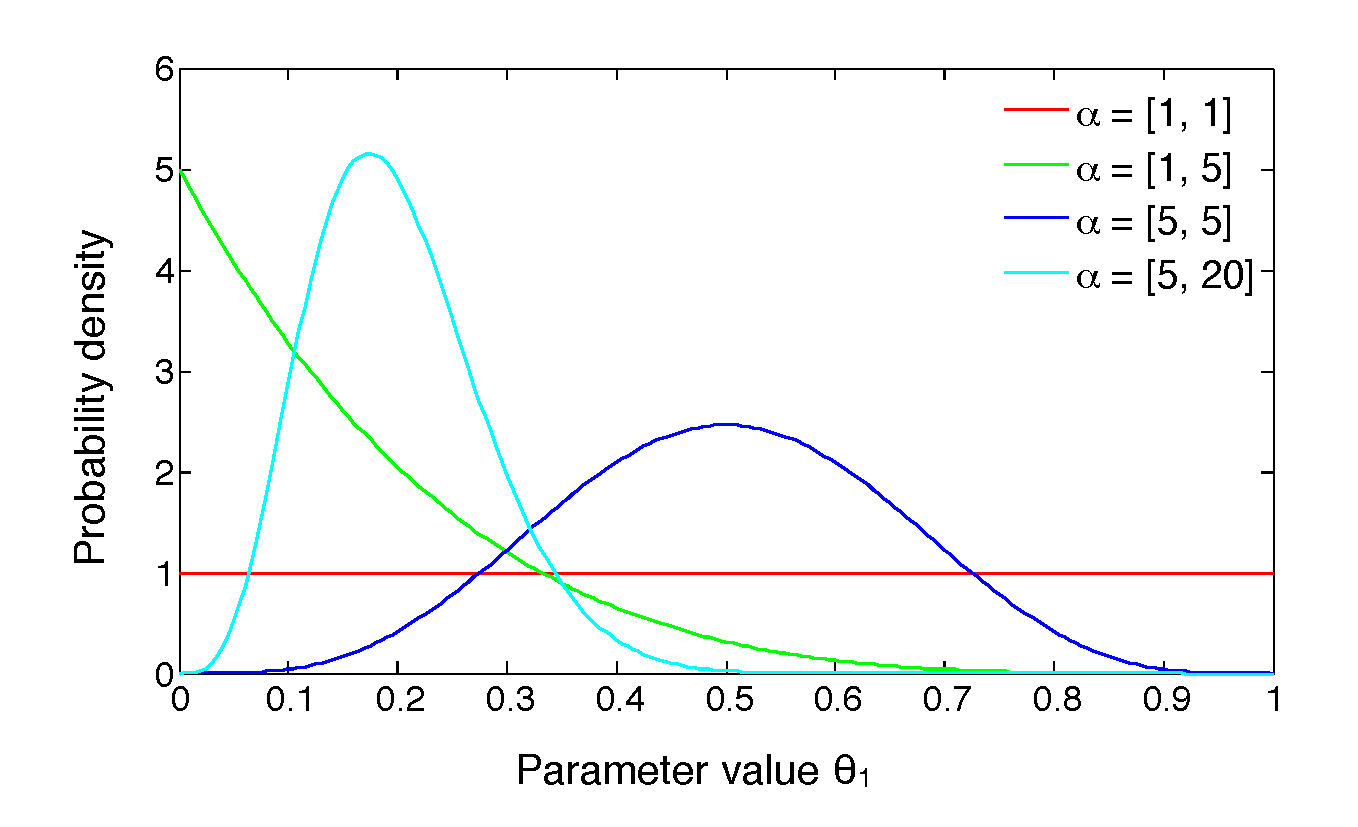
\includegraphics[scale=0.45]{imgs/dirichletfun.pdf}
\caption{Probability density functions for the Dirichlet distribution $P(\theta_1 \,; \boldsymbol\alpha)$  according to various values for the $\boldsymbol\alpha$ hyper-parameters.}
\label{fig:dirichletfun}
\end{figure}

As Dirichlet distributions are conjugate priors of categorical distributions, their posterior distribution after the observation of their corresponding variable remains a Dirichlet distribution with updated counts. As an illustrative example, the posterior distribution of $\boldsymbol\theta_{r_{1}(1)}$ after observing a fire when $\mathit{Rain}\!=\!\mathit{false} \land \mathit{Weather}\!=\!\mathit{hot}$ can be derived from Bayes' rule: 
\begin{align}
&P(\boldsymbol\theta_{r_{1}(1)} \; | \; \mathit{Fire}'\!=\!\mathit{true}, \mathit{Rain}\!=\!\mathit{false}, \mathit{Weather}\!=\!\mathit{hot}) \nonumber \\
& = \eta \ P(\mathit{Fire}'\!=\!\mathit{true} \; | \; \mathit{Rain}\!=\!\mathit{false}, \mathit{Weather}\!=\!\mathit{hot}\,; \boldsymbol\theta_{r_{1}(1)}) \ P(\boldsymbol\theta_{r_{1}(1)}) \nonumber \\
& = \eta \ \theta_{r_{1}(1,1)} \ \mathrm{Dirichlet}(\alpha_1,\alpha_2) \nonumber \\
& = \eta' \ \theta_{r_{1}(1,1)} \ [ \theta_{r_{1}(1,1)}^{\alpha_1 - 1} \times \theta_{r_{1}(1,2)}^{\alpha_2 - 1} ]   = \eta' \ \textrm{Dirichlet}(\alpha_1+1,\alpha_2) \nonumber 
\end{align}

where $\eta$ and $\eta'$ are normalisation factors.  Given a prior probability distribution $P(\boldsymbol\theta_{r_{1}(1)}) \sim \mathrm{Dirichlet}(\alpha_1, \alpha_2)$, the posterior distribution for $\boldsymbol\theta_{r_{1}(1)}$ after the observation  $\mathit{Fire}\!=\!\mathit{true}$ is thus another Dirichlet distribution $\sim \mathrm{Dirichlet}(\alpha_1+1,\alpha_2)$.  This updated Dirichlet distribution results in a slightly higher probability for the occurrence of fire, reflecting the evidence provided by the observation. 

%As explained in Section \ref{sec:learning}, this property is, however, contingent on the full observability of the domain variables. 

%$For instance, we can encode the fact that the user is unlikely to change his intention after a clarification request by assigning a higher $\alpha$ value to the intention $i_u'$ corresponding to the current value $i_u$ when $a_m$ is a clarification request. 


\subsubsection*{Utility parameters}
\index{rule parameters!of utility rules}

The parameters of utility rules are also defined by probability density functions.  However, contrary to probability values, the values in a utility distribution are independent of one another and need not satisfy the probability axioms (their range of possible values is arbitrary). Each utility value $u_{(i,j)}$ assigned to decision $d_{(i,j)}$ is therefore associated with its own, univariate distribution.

Rule $r_{2}$ illustrates a utility rule with four independent parameters:
\begin{align*}
r_{2}: \ \ & \textbf{if} \ (\mathit{Fire}\!=\!\mathit{true}) \ \textbf{then} \\
& \;\;\;\;\;  \begin{cases}
U(\mathit{Tanker}'\!=\!\mathit{drop\mbox{-}water}) = \theta_{r_{2}(1,1)} \\
U(\mathit{Tanker}'\!=\!\mathit{wait}) = \theta_{r_{2}(1,2)}
\end{cases} \\
& \textbf{else} \\
& \;\;\;\;\; \begin{cases}
U (\mathit{Tanker}'\!=\!\mathit{drop\mbox{-}water}) = \theta_{r_{2}(2,1)} \\
U(\mathit{Tanker}'\!=\!\mathit{wait}) = \theta_{r_{2}(2,2)}
\end{cases}
\end{align*}

Several types of density functions can be applied to define the prior distributions over these utility values.  This thesis concentrates on two specific families of priors, one non-informative (uniform distributions) and one informative (normal distributions): \index{uniform distribution} \index{normal distribution}
\begin{enumerate}
\item Continuous uniform distributions are defined on an interval $[a,b]$ which corresponds to the allowed range of utility values, and have the following density:
\begin{equation}
P(\theta\,; a, b) = \begin{cases}
\frac{1}{b - a} & \text{for } \theta \in [a,b]  \\
0               & \text{otherwise}
\end{cases}
\end{equation}

\item Normal (also called Gaussian) distributions are defined by a probability density function revolving around a mean $\mu$ and variance $\sigma^2$:
\begin{equation}
P(\theta\,; \mu, \sigma^2) = \frac{1}{\sqrt{2\pi\sigma^2}}\operatorname{exp}\left\{-\frac{\left(\theta-\mu\right)^2}{2\sigma^2}\right\}
\end{equation}
The range of possible values can be further constrained by truncating the density function.

\end{enumerate}

Normal distributions are well suited to represent utility values for which rough initial estimates are available. If a particular utility value is expected to lie in the vicinity of a particular value, its probability distribution can be expressed via a normal distribution with a mean centred on this value and a variance reflecting the confidence in the provided estimate. 

Figure \ref{fig:uniformn} illustrates three instances of probability density functions for a parameter $\theta$.  The first distribution corresponds to a uniform distribution on the interval $[-2,4]$, while the second and third distributions are truncated normal distributions with mean $\mu=2$ and variances respectively assigned to $\sigma^2=4$ and $\sigma^2=1$ . The two normal distributions illustrate how prior knowledge about the utility value can be incorporated in the prior -- in this case, the distributions rest on the assumption that the true utility value is likely to revolve around the value 2. 

\begin{figure}[ht]
\centering
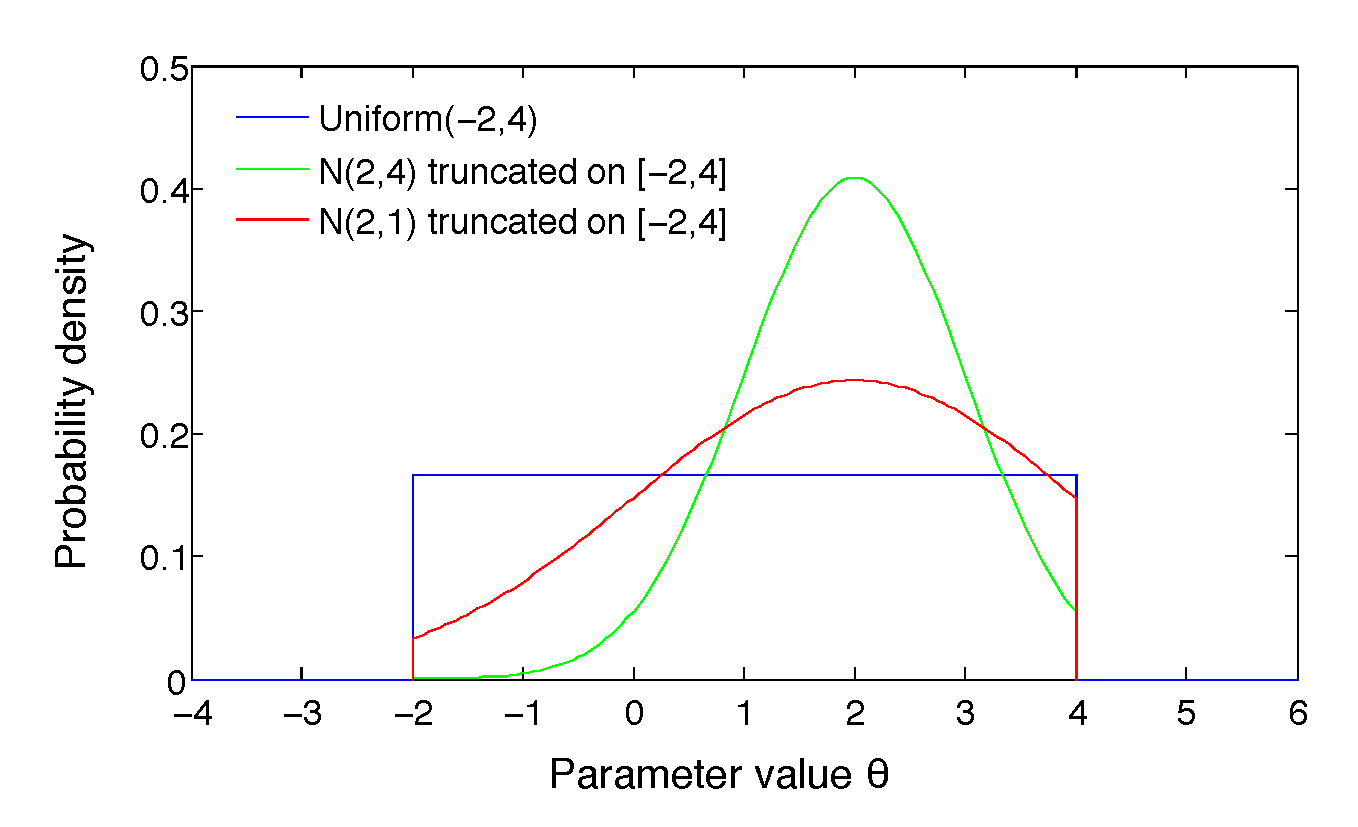
\includegraphics[scale=0.45]{imgs/uniformn.pdf}
\caption{Probability density functions $P(\theta)$ over the interval $[-2,4]$ using an uniform distribution, a truncated normal distribution $\mathcal{N}(2,4)$ and a truncated normal distribution $\mathcal{N}(2,1)$.} 
\label{fig:uniformn}
\end{figure}

\subsection{Instantiation}
\label{sec:rule-params-instantiation}

Parameters are instantiated in the dialogue state as chance nodes.  One distinct node is created for each (univariate or multivariate) parameter distribution and included as a parent of its corresponding rule node. The rule distributions defined in Section \ref{sec:ruleinstantiation} must be slightly adapted to account for these parameters in the parent nodes of the rule.  The rest of the instantiation process remains unchanged. 

\subsubsection*{Parameters of probability rules}

A parametrised probability rule $r$ structured with $n$ conditions is associated with $n$ multivariate parameter nodes $\boldsymbol\theta_{r(1)}, \dots, \boldsymbol\theta_{r(n)}$.  Each distribution $P(\boldsymbol\theta_{r(i)})$ is a Dirichlet distribution of dimension $m_i$, where $m_i$ is the number of effects associated with the condition $c_i$ (including the empty effect). Figure \ref{fig:ruleinstantiation_params} illustrates this instantiation procedure with two probability rules.  

The conditional probability distribution of a rule node $r$ given its input variables $I_1, \dots, I_k$ and parameters $\boldsymbol\theta_{r(1)}, \dots, \boldsymbol\theta_{r(n)}$ is a straightforward adaptation of Equation \eqref{eq:ruledistrib}:
\begin{align}
& P(r\!=\!e \, | \, I_1\!=\!i_1, \dots,  I_k\!=\!i_k\,; \boldsymbol\theta_{r(1)}, \dots, \boldsymbol\theta_{r(n)})  = P(E_i = e\,; \boldsymbol\theta_{r(i)}) \\
& \; \; \; \; \; \; \; \; \text{ where } i = \min_i (c_i \text{ is satisfied with } I_1\!=\!i_1 \land \dots \land I_k\!=\!i_k) \nonumber
\end{align}

\subsubsection*{Parameters of utility rules}

The parameters of utility rules are instantiated in a similar manner, as shown in Figure \ref{fig:ruleinstantiation_params2}. The corresponding utility distribution is adapted from Equation \eqref{eq:utildistrib} as follows:
\begin{align}
& U_r(I_1\!=\!i_1, \dots, I_k\!=\!i_k, A_1'\!=\!a_1, \dots, A_l'\!=\!a_l\,; \boldsymbol\theta_{r(1)}, \dots, \boldsymbol\theta_{r(n)}) \nonumber \\ 
& = U_i(A_1'\!=\!a_1, \dots, A_l'\!=\!a_l\,; \boldsymbol\theta_{r(i)})  \label{eq:utildistrib_params}\\
& \; \; \; \; \; \; \; \; \text{ where } i = \min_i (c_i \text{ is satisfied with } I_1\!=\!i_1 \land \dots \land I_k\!=\!i_k) \nonumber
\end{align}

\begin{figure}[h!]
\centering
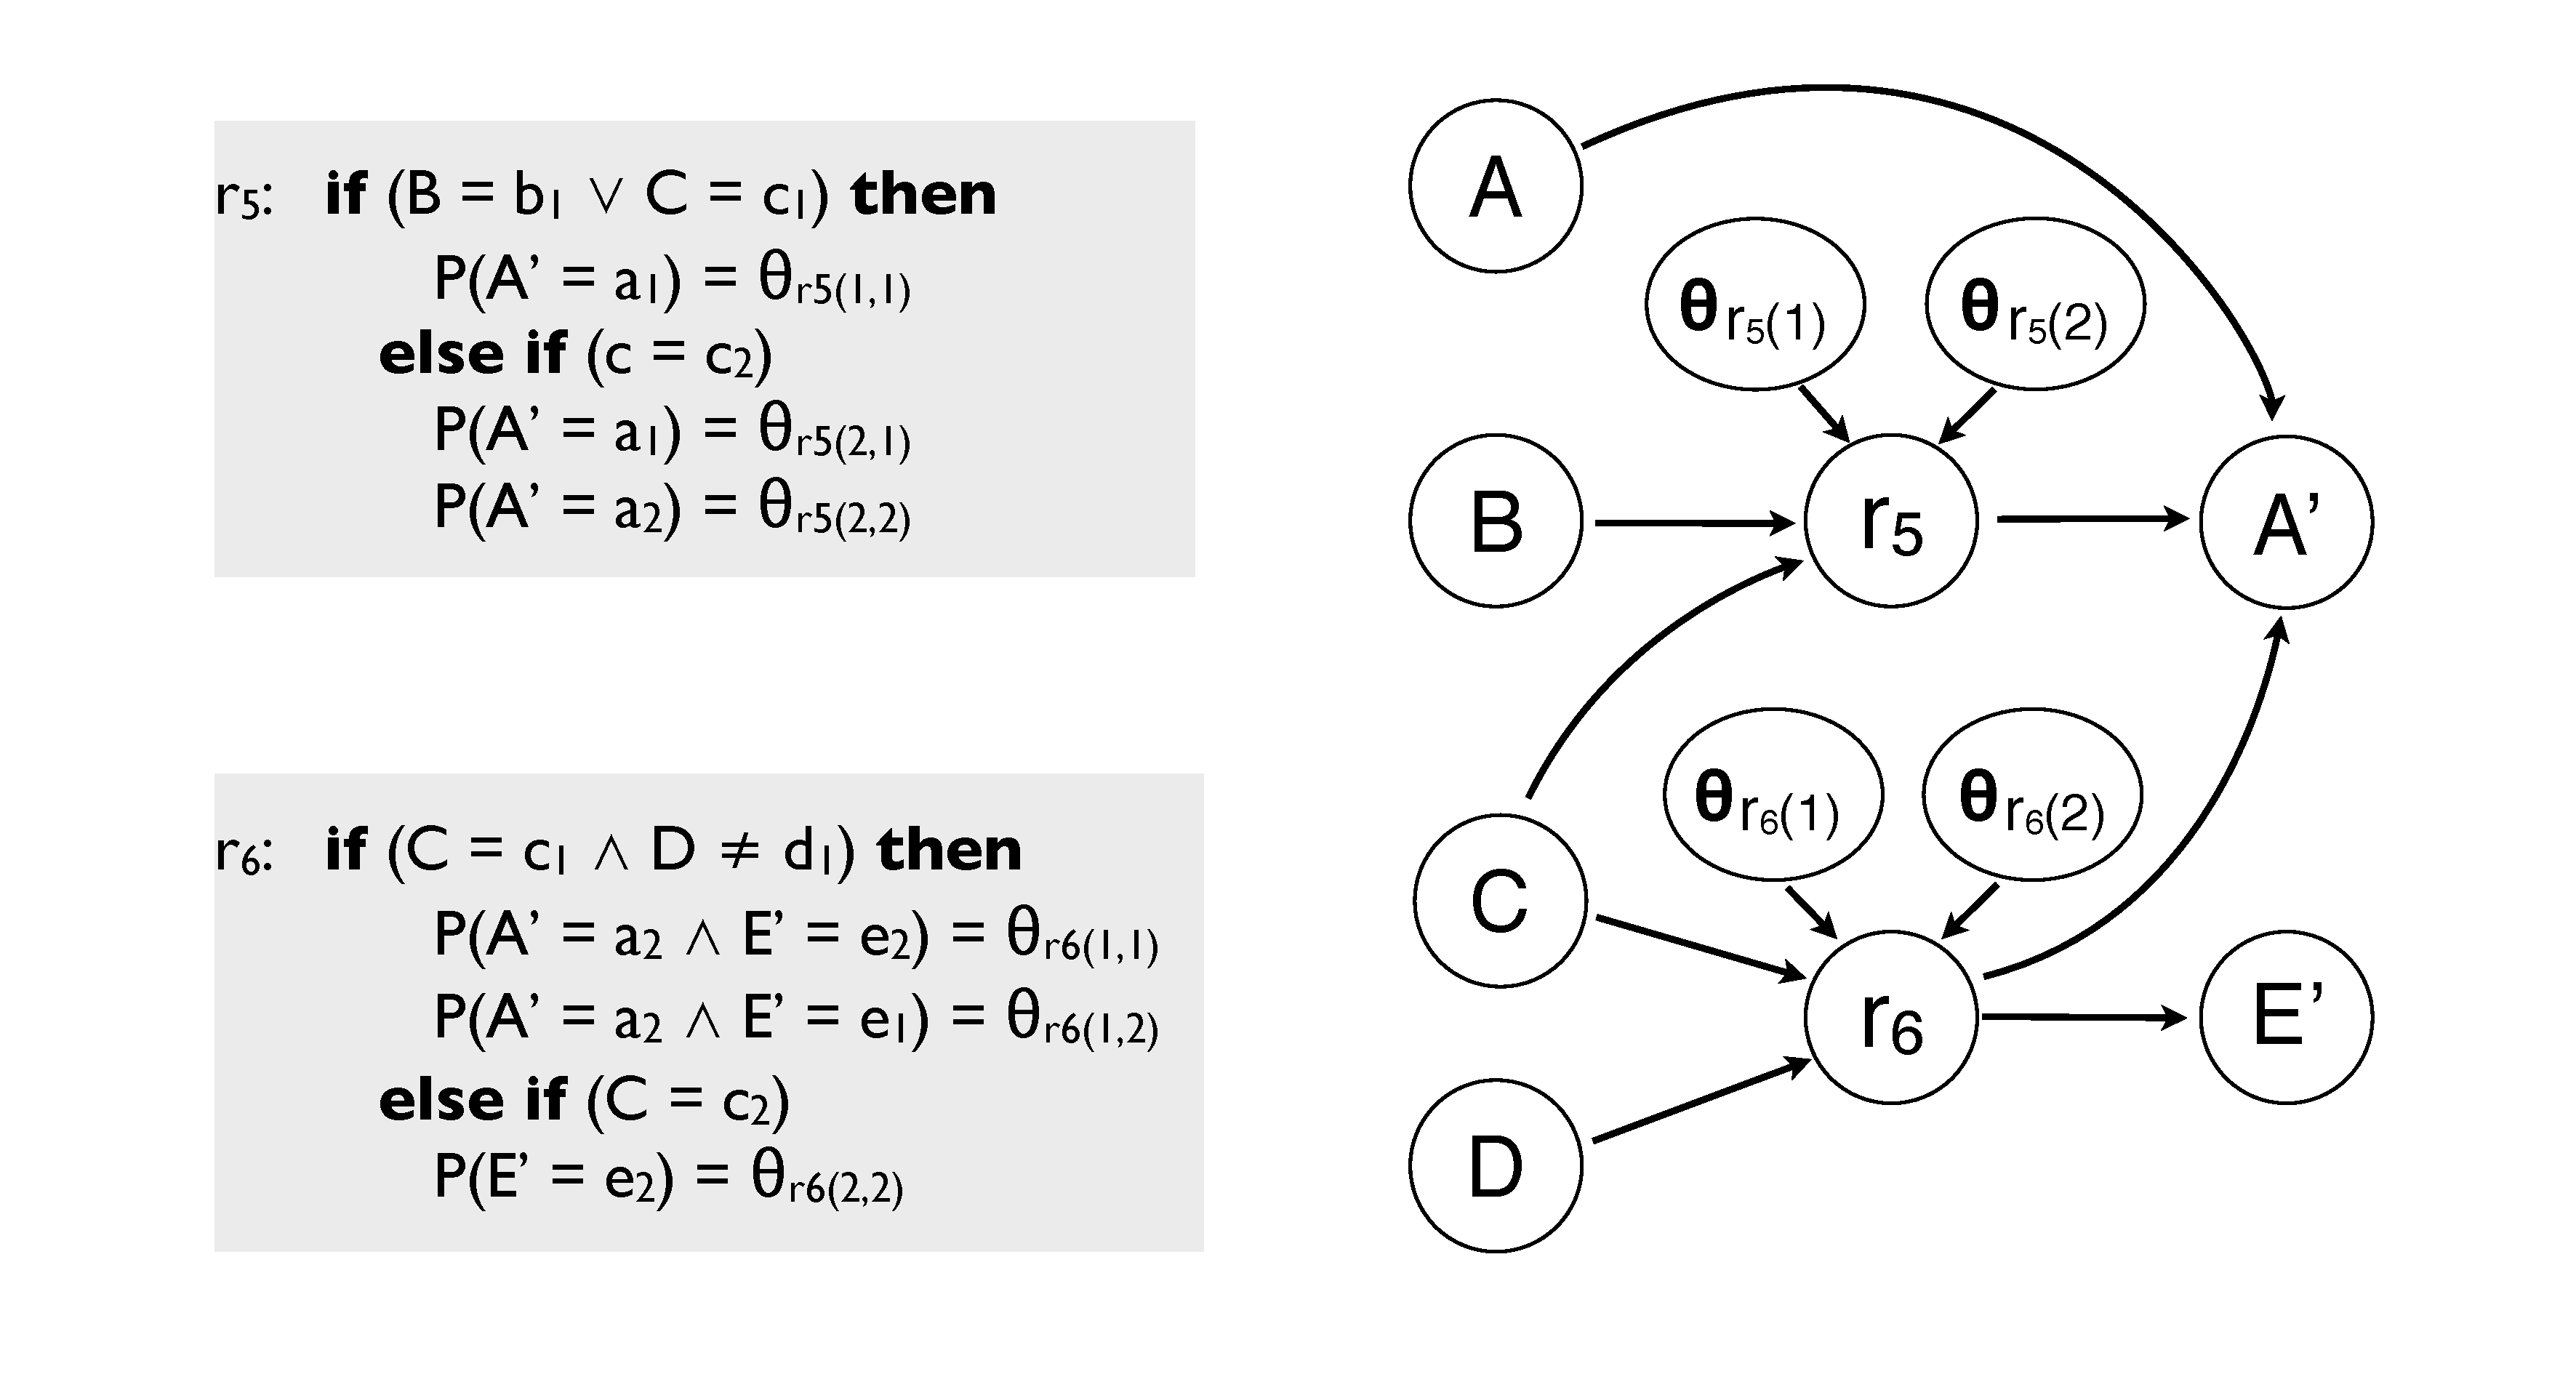
\includegraphics[scale=0.25]{imgs/ruleinstantiation_params.pdf}
\caption{Example of instantiation for two parametrised probability rules $r_5$ and $r_6$.}
\label{fig:ruleinstantiation_params}
\end{figure}


\begin{figure}[h!]
\centering
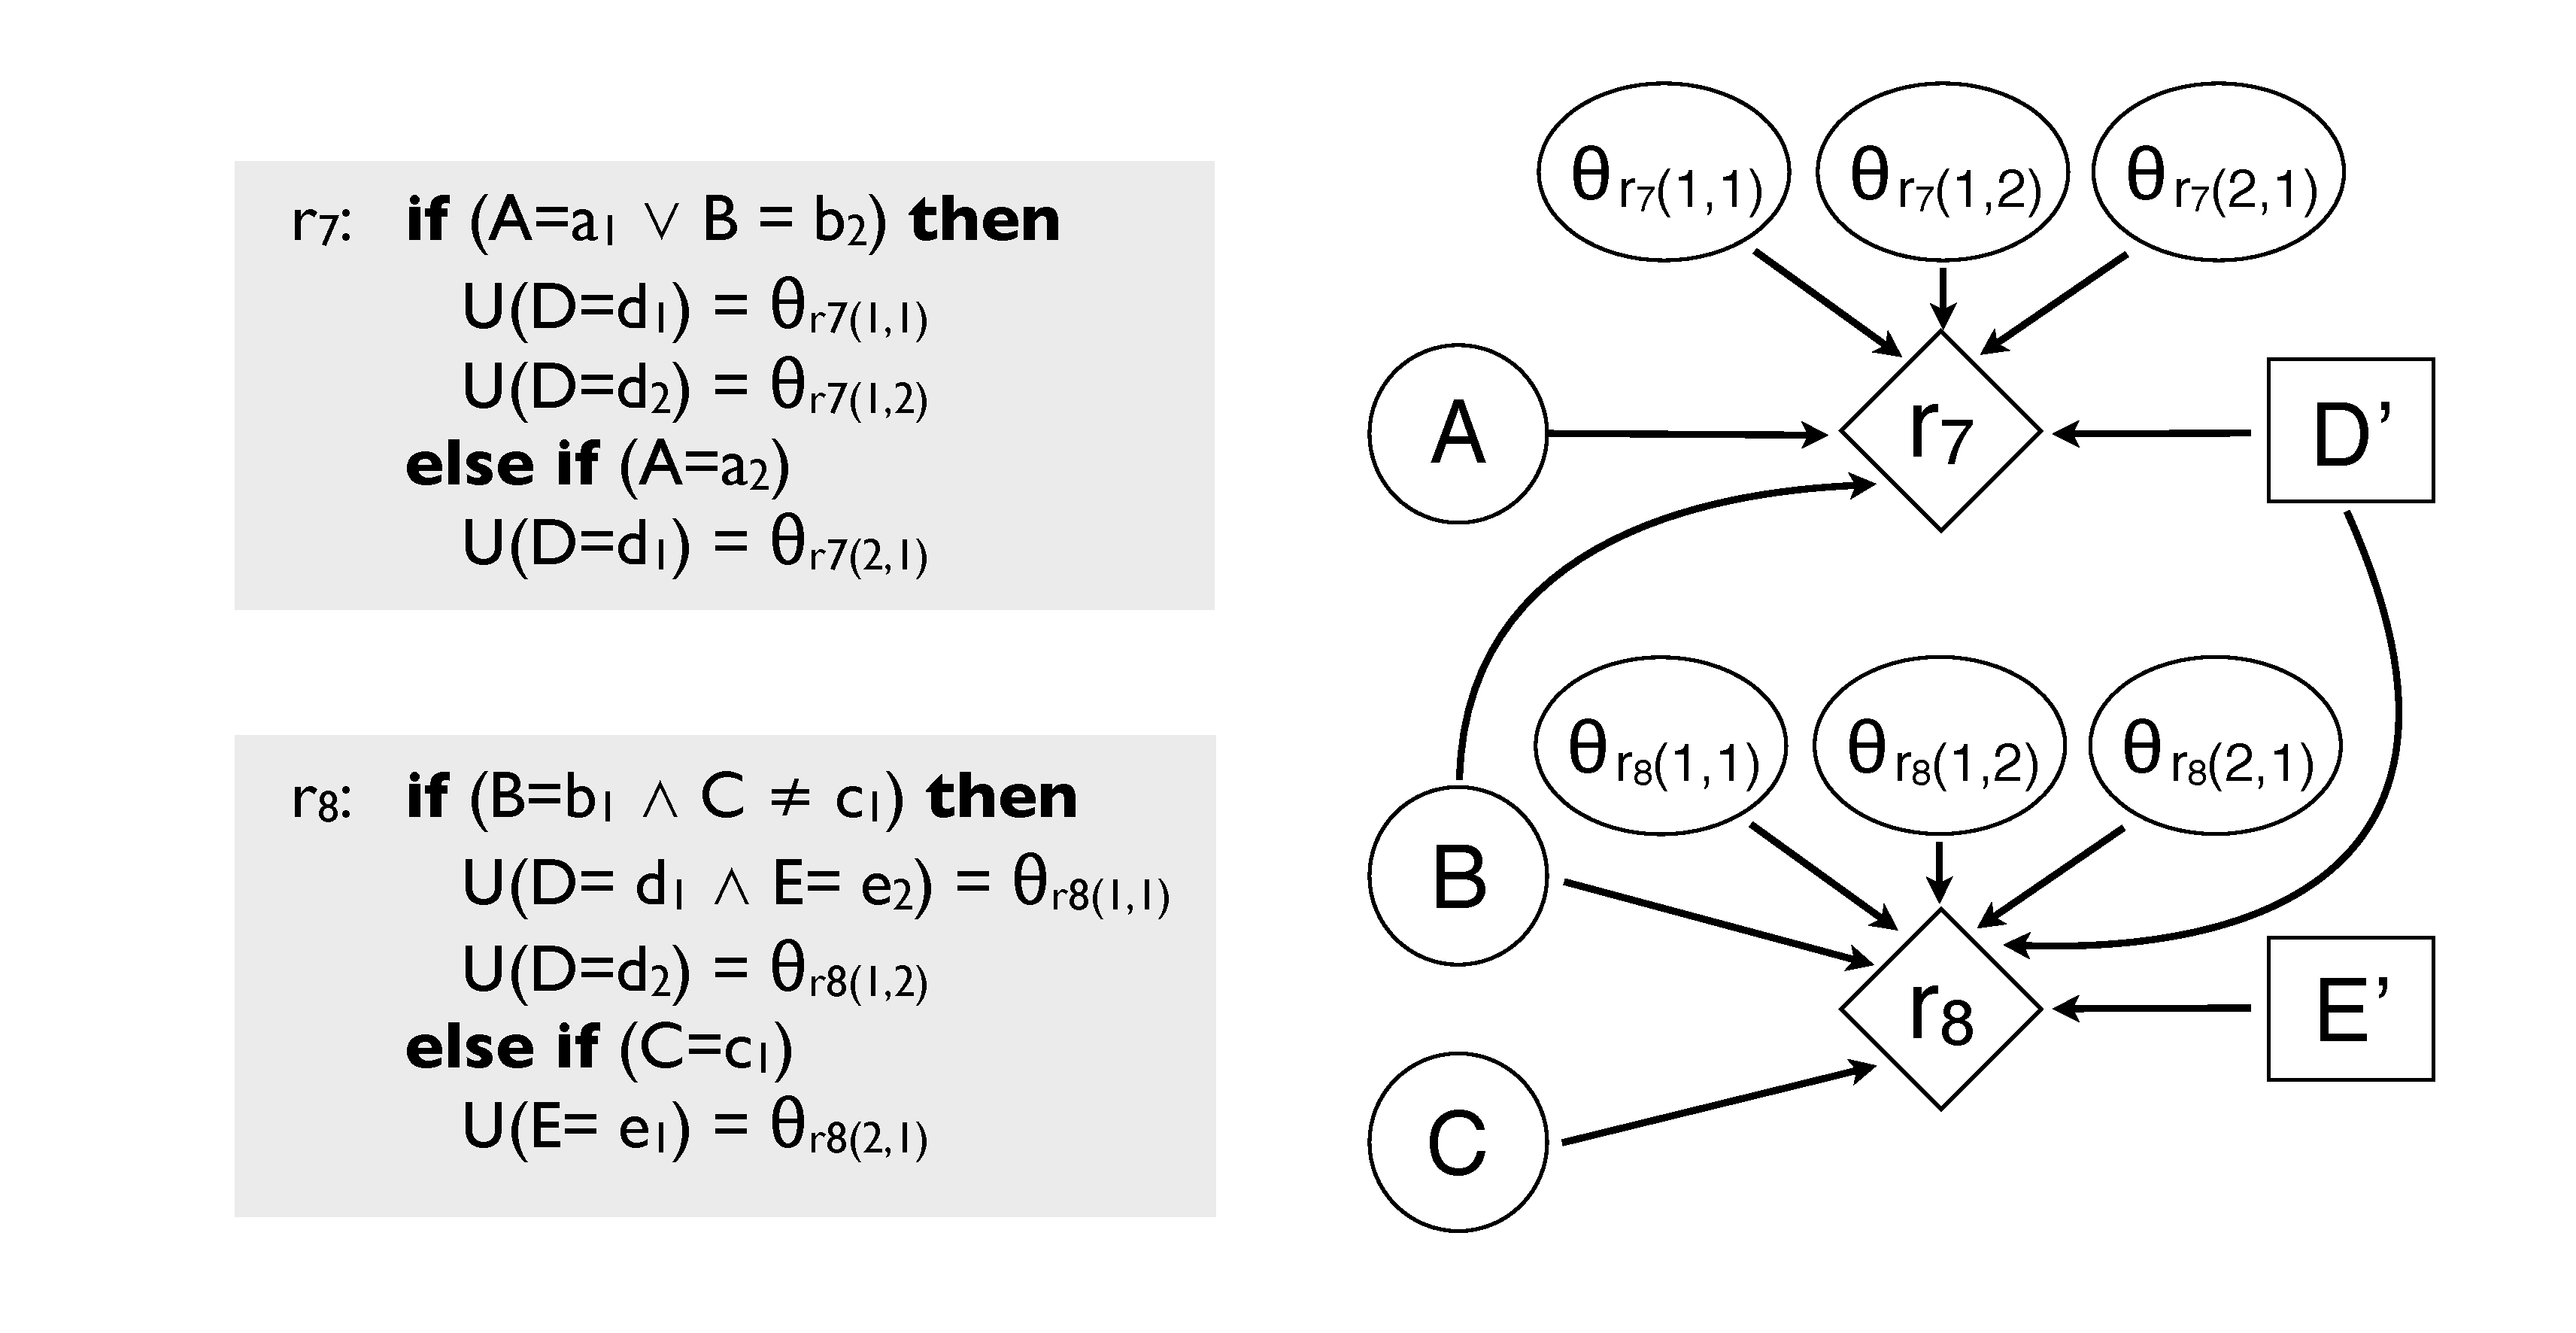
\includegraphics[scale=0.25]{imgs/ruleinstantiation2_params.pdf}
\caption{Example of instantiation for two parametrised utility rules $r_7$ and $r_8$.}
\label{fig:ruleinstantiation_params2}
\end{figure}

\section{Supervised learning of rule parameters}
\label{sec:rule-supervised}
\index{rule parameters!supervised learning of}
\index{supervised learning}

Once the rule parameters are instantiated as nodes in the dialogue state, one can calculate their posterior distribution $P(\boldsymbol\theta \, | \, \mathcal{D})$ after observing a particular data set $\mathcal{D}$ using standard algorithms for probabilistic inference. The estimation of rule parameters corresponds to a learning problem with partial data (cf. Section \ref{sec:learning}), since some of the nodes in the dialogue state  -- such as rule nodes -- are not directly observed. The posterior distribution $P(\boldsymbol\theta \, | \, \mathcal{D})$ is thus no longer guaranteed to remain in the same distribution family as their prior distributions.  The solution adopted here is to approximate the parameter distributions via sampling techniques.
The estimation of rule parameters from data is practically achieved by cycling through the data sample one after the other and gradually refining the parameter distributions in the light of the observed values. We describe in the next pages the generic representation of the training data as well as the learning algorithm employed for the estimation of rule parameters given some reasonable assumptions about the wizard behaviour.  
\subsection{Wizard-of-Oz training data}
\label{sec:rule-supervised-oz}
\index{Wizard-of-Oz interaction|textbf}

The focus of this chapter is on the estimation of rule parameters from a specific type of training data, namely Wizard-of-Oz interactions. Wizard-of-Oz interactions are interactions between human users and a dialogue system which is remotely controlled by a human expert ``behind the curtains''.  They constitute a simple and efficient method to collect realistic conversational behaviour for a particular domain in the absence of a fully implemented or optimised system.\footnote{Developing spoken dialogue systems can indeed lead to a classical ``chicken-and-egg'' dilemma: In order to build up a particular system, system designers often need to know what types of user utterances and behaviours are expected -- but in order to collect such data, one must first have an integrated dialogue system with which the users can interact.  Wizard-of-Oz interactions are a way to circumvent this dilemma.}

%We describe below the representation format used to encode these interactions and how domain models can be optimised given some reasonable assumptions about the wizard behaviour. 

\subsubsection*{Representation format}

For the specific purpose of estimating the parameters of dialogue management models, we can represent Wizard-of-Oz interactions as a sequence of state--action pairs $\mathcal{D} = \{\langle \mathcal{B}_i, a_i \rangle : 1 \leq i \leq n\}$, where $\mathcal{B}_i$ corresponds to the dialogue state at time $i$, and $a_i$ is the associated action performed by the wizard.  The number $n$ corresponds to the total number of recorded actions. 
\index{dialogue state}
The dialogue state $\mathcal{B}_i$ represents the current conversational situation at time $i$ as it was perceived by the wizard.  The dialogue state usually includes the recent dialogue history as well as important contextual features.  As explained in the previous chapter, the dialogue state can be encoded as a Bayesian network to reflect state uncertainty and dependencies amongst state variables. Associated to each dialogue state is the corresponding action $a_i$ selected by the wizard at that state. This action can be void if the wizard decides to take no action at that specific step in the dialogue. 

%The sequence of state-action pairs $\mathcal{D}$ is in our approach automatically extracted from the collected interactions, without any manual annotation.  

Many conversational situations allow for multiple, equally ``correct'' system responses.  This characteristic of verbal interactions carries over to the state--action pairs of Wizard-of-Oz data sets, as one can occasionally observe similar states mapped to different wizard actions. The wizard actions should therefore be viewed as an indication of good conversational behaviour, but do not constitute absolute gold standards in the traditional sense of being the uniquely appropriate output for the given dialogue state. The existence of multiple responses also entails that the accuracy of the learned models remains contingent on the degree of internal consistency of the wizard actions. 

\subsubsection*{Assumptions about the wizard behaviour}
\index{Wizard-of-Oz interaction!assumptions about}

Parameter estimation on Wizard-of-Oz data rests on the assumption that the wizard is a rational agent and will tend to select actions that are deemed most useful in their respective dialogue state. It should be stressed that the agent is only assumed to act rationally \textit{given} the perceived (uncertain) dialogue state. The wizard must indeed act on the basis of ``noisy'' inputs (including e.g.\ speech recognition errors) and may as a consequence select suboptimal actions if the provided inputs contain erroneous hypotheses. It should therefore be stressed that the assumption of rationality does not equate to an assumption of omniscience on the part of the wizard.  

In practice, the posited rationality of the wizard implies that the likelihood $P_{\mathcal{B}_i}(a_i\,; \boldsymbol\theta)$ of a wizard action $a_i$ in a particular dialogue state $\mathcal{B}_i$ under the parameters $\boldsymbol\theta$ will depend on the utility of action $a_i$ in $\mathcal{B}_i$ relative to other possible actions (as formalised below).

\subsection{Learning cycle}
\label{sec:rule-supervised-learning}
\index{supervised learning!as imitation}

The goal of the learning process is to estimate the posterior distribution $P(\boldsymbol\theta \, | \, \mathcal{D})$ over the rule parameters given the collected Wizard-of-Oz data set. The procedure operates in an incremental fashion by traversing the state--action pairs one by one and updating the posterior parameter distributions after each pair.  

\subsubsection*{Likelihood distribution}
 \index{likelihood distribution}
One key element of the learning cycle is the definition of the probability $P_{\mathcal{B}_i}(a_i\,; \boldsymbol\theta)$, which specifies the likelihood of the wizard action $a_i$ in a dialogue state $\mathcal{B}_i$ given the parameters $\boldsymbol\theta$. The intuitive purpose of this likelihood is to favour the parameter values that provide a good fit for the wizard action choices. In practice, this is achieved by representing the likelihood of the wizard action $a_i$ in terms of the relative utility of action $a_i$ compared to alternative action choices. The first step is to calculate the utility $U_{\mathcal{B}_i}(a\,; \boldsymbol\theta)$ for all possible actions $a$, and to subsequently rank the actions in descending order of utility.  As the wizard is presupposed to act rationally in most cases, the wizard action is expected to appear at the top of this ranked list of actions. Formally, the likelihood of action $a_i$ given the parameters $\boldsymbol\theta$ is expressed as:
\begin{align}
P_{\mathcal{B}_i}(a_i\,; \boldsymbol\theta) & = \begin{cases} \eta \, p & \text{if } a_i \ \text{ is the action with highest utility given } \boldsymbol\theta  \\
\eta (1-p) p & \text{ if } a_i \ \text{is the second-highest action} \\
\eta (1-p)^2 p & \text{ if } a_i \ \text{is the third-highest action} \\ 
\dots
\end{cases} \nonumber \\[3mm]
& = \ \ \eta (1-p)^x p \ \ \ \ \ \ \ \text{ where } x \text{ is the position of action } a_i \label{eq:likelihood1} \\ 
&  \phantom{= (1-p)^x p} \ \ \ \ \ \ \ \ \ \ \ \text{ in the ranked list of actions}  \nonumber
\end{align}

The $\eta$ factor in Eq. \eqref{eq:likelihood1} represents as usual the normalisation factor, while the probability $p$  represents the learner confidence in the judgement of the wizard.  A value $p = 0.7$ will hence indicate that the wizard is assumed to act rationally -- and thus select the highest-utility action -- with probability $0.7$. The probability $p$ indirectly defines the learning rate of the estimation process: the higher the probability, the faster the learner will converge to a policy that imitate the wizard actions.  However, a high value for $p$ renders the learner more vulnerable to the occasional errors and inconsistencies on the part of the wizard. 


\begin{wrapfigure}[18]{r}{65mm}
\vspace{-2mm}
\centering
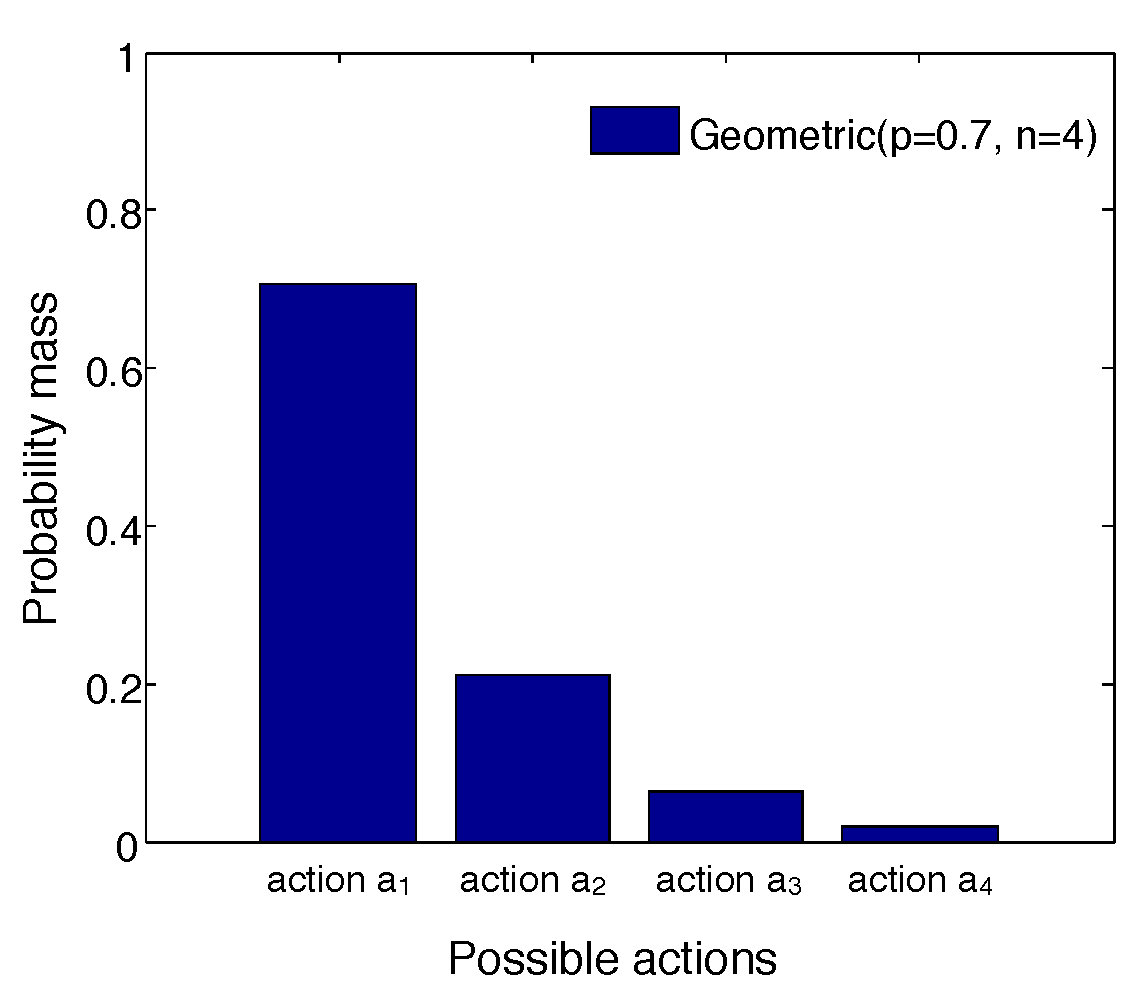
\includegraphics[scale=0.34]{imgs/geometric.pdf} 
\vspace{-6mm}
\caption{Distribution $P_{\mathcal{B}_i}(a_i\,; \boldsymbol\theta)$ for four action values $[a_1, a_2, a_3, a_4]$ ranked by decreasing utility, with $p=0.7$.}
\label{fig:geometric}
\end{wrapfigure}
\index{geometric distribution}
The probability distribution represented by Equation \eqref{eq:likelihood1} is a particular instance of a \textit{geometric} distribution.\footnote{Technically speaking, the definition in Equation \eqref{eq:likelihood1} corresponds to a truncated version of the geometric distribution, as the support of the distribution is finite (the number of possible actions is bounded). The reduction of the distribution to a finite support is achieved via the normalisation factor $\eta$.} Geometric distributions correspond to the number of Bernoulli trials required to get one success. The reliance on geometric distributions to formalise the likelihood of the observed actions is motivated by the posited rationality of the wizard decisions.  In other words, the formalisation is grounded in the assumption that the wizard will select the highest utility action with probability $p$, the second-highest action with probability $(1-p)p$, and so forth. The geometric distribution is monotonically decreasing, which ensures that the probability of a high-utility action will always be higher than its lower-utility alternatives.   Figure \ref{fig:geometric} illustrates an example of likelihood distribution over four action values $[a_1, a_2, a_3, a_4]$, where $U_{\mathcal{B}_i}(a_1\,; \boldsymbol\theta) > U_{\mathcal{B}_i}(a_2\,; \boldsymbol\theta) > U_{\mathcal{B}_i}(a_3\,; \boldsymbol\theta) > U_{\mathcal{B}_i}(a_4\,; \boldsymbol\theta)$.


\subsubsection*{Posterior parameter distribution}
\index{posterior distribution}
Given the aforementioned likelihood distribution, the posterior distribution over the parameters is defined via Bayes' rule: 
\begin{equation}
P_{\mathcal{B}_i}(\boldsymbol\theta \, | \, a_i) = \eta \, P_{\mathcal{B}_i}(a_i\,; \boldsymbol\theta) \, P(\boldsymbol\theta ) \label{eq:paramposterior}
\end{equation}

The factor $\eta$ is used for normalisation. The calculation of this posterior distribution is a non-trivial inference problem as the probabilistic model contains both continuous and discrete random variables.  Two types of solutions can be distinguished:
\begin{itemize}
\item The first strategy is to discretise the range of parameter values into distinct, mutually exclusive buckets, and thereby transform continuous variables into discrete variables, with a number of values equivalent to the number of buckets employed for the discretisation.
\item The second strategy is to retain the continuous nature of the parameters, but approximate the inference process through the use of sampling techniques.  
\end{itemize}
\index{probability distribution!discretisation of}\index{sampling techniques}
Although both solutions are implemented in the \opendial{} toolkit, sampling techniques such as likelihood weighting have in practice proved to be more efficient and scalable than discretisation. 

After sampling, the full joint distribution $P_{\mathcal{B}_i}(\boldsymbol\theta \, | \, a_i)$ is factored into the individual parameter variables. This factorisation corresponds to a simplifying assumption as parameter independence is theoretically no longer guaranteed when handling partially observed data. 
%:\begin{equation}
%P_{\mathcal{B}_i}(\boldsymbol\theta | a_i) = \prod_{\theta_j \in \boldsymbol\theta} P_{\mathcal{B}_i}(\theta_j | a_i)
%\end{equation}

\subsubsection*{Representation of the posterior}

The result of the posterior calculation in Equation \eqref{eq:paramposterior} is a collection of sampled values. In order to derive a full probability density function from these samples, one can either follow a so-called parametric approach and seek to reconstruct the underlying parametric distributions (such as Gaussian or Dirichlet distributions) that best fit the data, or adopt a non-parametric strategy and directly represent the posterior as a function of the collected samples. Parametric approaches, albeit interesting, are difficult to apply in this setting, for two main reasons:
\begin{enumerate}\index{non-parametric distribution}
\item The distribution family of the posterior is hard to determine, as the posterior is no longer ensured to remain in the same family as the prior when learning from partial data.  
\item Additionally, fitting multivariate distributions such as Dirichlets based on sampled values is a laborious computational process with no closed-form solutions.\footnote{Numerical methods based on fixed-point and Newton-Raphson iterations do exist, however \citep{minka2003}.}
\end{enumerate}

We have consequently adopted a non-parametric representation of the posterior distributions, based on \textit{kernel density estimation}\index{kernel density estimation} (KDE).  The kernel density estimator for a continuous variable $X$ for which a set of samples $x_1, \dots, x_n$ is available is given by:
\begin{equation}
P(x) = \frac{1}{nh} \sum_{i=1}^n K\Big(\frac{x-x_i}{h}\Big) \label{eq:kde}
\end{equation}
where $K(\cdot)$ is a \textit{kernel function}\index{kernel function} and $h$ is a smoothing parameter called the \textit{bandwidth}. Multiple kernel functions can be used, but a common choice is to adopt a Gaussian kernel. The kernel density estimator corresponds in this case to a combination of $n$ Gaussians, where each Gaussian is centred on a sample point $x_i$.  This combination of Gaussians is smoothed proportionally to the bandwidth parameter. Figure \ref{fig:kde} illustrate the use of kernel density estimation for a continuous variable based on a set of 50 samples and a Gaussian kernel. The figure shows the influence of the bandwidth parameter on the shape of the resulting density function. Kernel density estimators do not necessitate any particular assumption about the nature of the underlying distribution, and are therefore well-suited to represent distributions of indeterminate type -- as is the case for posterior distributions over the parameters of probabilistic rules. 

\begin{figure}[ht]
\centering
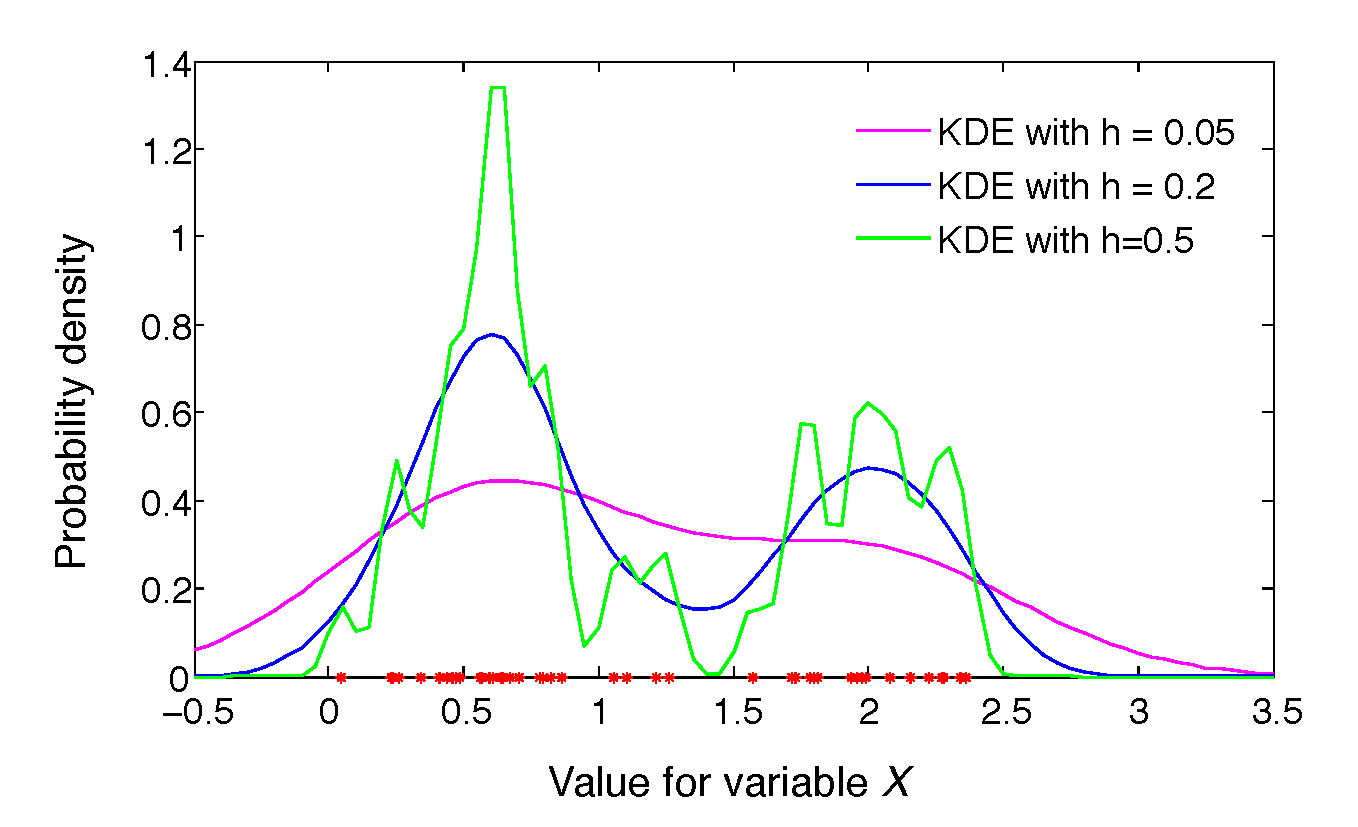
\includegraphics[scale=0.45]{imgs/kde.pdf} 
\caption{Kernel density estimators (KDEs) for a continuous variable $X$ based on 50 samples (shown on the X axis). The density function is shown for three possible bandwidths $h$. }
\label{fig:kde}
\end{figure}

Multivariate distributions are encoded with a multivariate extension of KDE based on product kernels \citep{Silverman1986}.  All estimators in our experiments employ Gaussian kernels with a bandwidth tuned from the sample variance using Silverman's rule of thumb \citep{Silverman1986}. 


\subsubsection*{Learning algorithm}

Algorithm \ref{algo:wozlearning} presents the general procedure for estimating model parameters from Wizard-of-Oz data.  The algorithm loops on each instance pair in the training data.   The posterior parameter distribution is estimated via sampling, based on the likelihood of the wizard action (line 2).  The individual posterior distributions for each parameter are then reconstructed via kernel density estimation on the sampled values (line 3-5), and the process is repeated. 

%For each pair, the algorithm starts by including the parameters in the dialogue state and triggering the domain models (line 2 and 3).

\begin{algorithm}[h!]
\caption{: \textsc{WoZ-learning} ($\mathcal{M}, \boldsymbol\theta, \mathcal{D}, N$)}
\begin{algorithmic}[1] \vspace{1mm}
\REQUIRE Rule-structured models $\mathcal{M}$ for the domain
\REQUIRE Model parameters $\boldsymbol\theta$ with prior distribution $P(\boldsymbol\theta)$
\REQUIRE Wizard-of-Oz data set $\mathcal{D} = \{\langle \mathcal{B}_i, a_i \rangle : 1 \leq i  \leq n\}$
\REQUIRE Number $N$ of samples to draw for each learning example
\ENSURE Posterior distribution $P(\boldsymbol\theta \; | \; \mathcal{D})$ for the parameters  \vspace{1mm}
\FORALL {$\langle \mathcal{B}_i, a_i \rangle \in \mathcal{D}$}
%\STATE Set $\mathcal{B}_i \leftarrow \mathcal{B}_i \cup \boldsymbol\theta$
%\STATE $\mathcal{B}_i, \mathbf{e} \leftarrow$ \textsc{TriggerModels} ($\mathcal{B}_i, \emptyset,  \mathcal{B}_i$) 
%\STATE Let $U_{\mathrm{min}}$ be the minimal threshold for the utilities in $\mathcal{B}_i$ \vspace{2mm} 
%\STATE Define likelihood  $P_{\mathcal{B}_i}(a_i\,; \boldsymbol\theta) \leftarrow \dfrac{U_{\mathcal{B}_i}(a_i\,; \boldsymbol\theta) - U_{\mathrm{min}}}{\sum_{a \in \mathit{Val}(A)} \left(U_{\mathcal{B}_i}(a\,; \boldsymbol\theta) - U_{\mathrm{min}}\right)} $ \vspace{2mm} 
\STATE Draw $N$ samples $\mathbf{x}_1, \dots, \mathbf{x}_N$ from posterior $P_{\mathcal{B}_i}(\boldsymbol\theta \, | \, a_i) = \eta \, P_{\mathcal{B}_i}(a_i\,; \boldsymbol\theta) \, P(\boldsymbol\theta )$
\FORALL {parameter variable $\theta \in \boldsymbol\theta$}
\STATE Set $P(\theta) \leftarrow \mathrm{KDE}(\mathbf{x}_1(\theta), \dots, \mathbf{x}_N(\theta))$
\ENDFOR
\ENDFOR
\RETURN $P(\boldsymbol\theta)$
\end{algorithmic}
\label{algo:wozlearning}
\end{algorithm}


\section{Experiments}
\label{sec:wozlearning-experiments}

We evaluated the learning approach outlined in this chapter in the context of a dialogue policy learning task for a human--robot interaction scenario.  The goal of the experiment, originally presented in \cite{rulebasedmodels-sigdial2012}, was to evaluate whether the parameters of a rule-structured utility model could be efficiently optimised from small amounts of Wizard-of-Oz data.  The evaluation metric was defined in this experiment as the proportion of actions corresponding to the wizard selections. The rule-structured model was compared to two baselines encoding the action utilities via traditional representations (plain utility tables and linear functions, respectively). \index{Wizard-of-Oz interaction!agreement measure}

%The empirical results showed that the model encoded with utility rules were able to reproduce the wizard policy  than the more weakly structured baseline models. 

It should be stressed that the purpose of the experiment is limited to the evaluation of the \textit{learning performance}\index{learning performance} of the model. The evaluation of the model in terms of e.g.\ qualitative and quantitative metrics of interaction success (and user satisfaction) constitutes an important but separate question, which will be addressed in Chapter \ref{chap:user-evaluation}. 

We first describe in this section the dialogue domain employed for the experiment, after which we detail the data collection procedure and experimental setup, and finally present and analyse the empirical results. 

\subsection{Dialogue domain}
\label{sec:wozlearning-experiments-domain}
\index{dialogue domain}

The scenario for the Wizard-of-Oz experiment involved a human user and a Nao robot (nicknamed ``Lenny''), which is a programmable humanoid robot developed by Aldebaran Robotics. Figure \ref{fig:nao2} shows a human user interacting with the robot during a data collection experiment. \index{human--robot interaction}\index{Nao robot}

\begin{figure}[ht]
\begin{center}
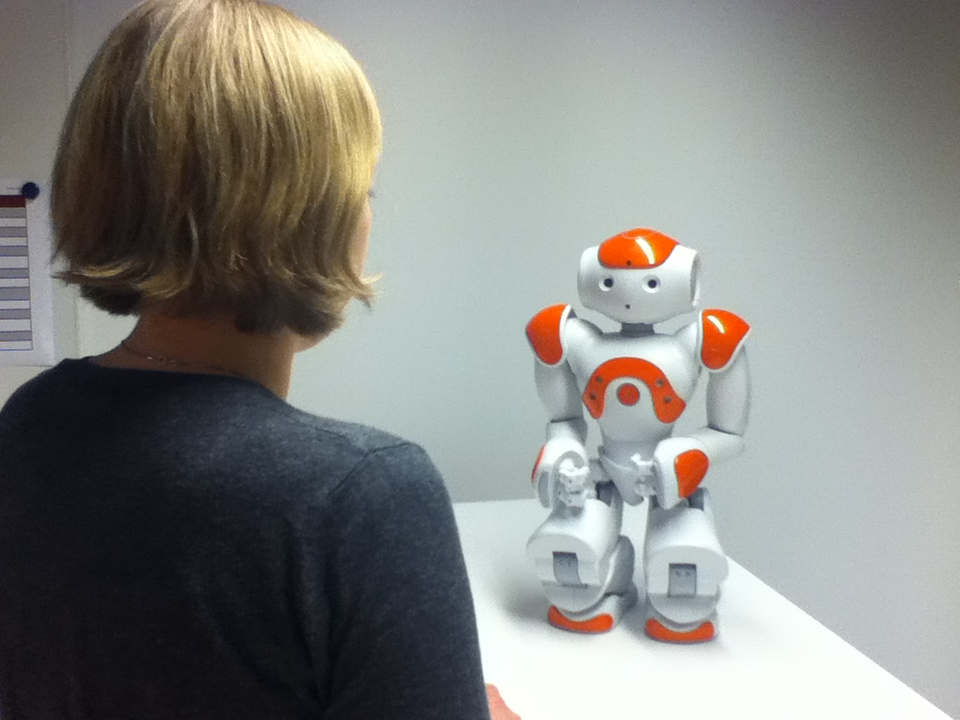
\includegraphics[scale=0.25]{imgs/bilde.jpg}
\end{center}
\caption{Human user interacting with the Nao robot during the Wizard-of-Oz data collection.}
\label{fig:nao2}
\end{figure}

The users were instructed to teach the robot a sequence of body movements such as lifting arms, stepping forward, backward, kneeling down, etc.  The movements could be performed either in consecutive order or in parallel (provided the movements were not in conflict).  The users were free to decide on the movements to perform, and communicated their intention using spoken commands (no gesture recognition was here involved).  The robot was programmed to memorise the instructed sequence and could ``replay'' it at any time.

The list of possible dialogue acts\index{dialogue acts} for the user is shown in Table \ref{table:userdas}, and includes a total of 16 dialogue act templates (expanding into 41 dialogue acts when counting all possible argument instantiations). The set of user dialogue acts contain both task-specific dialogue moves to convey user commands as well as conversational actions for feedbacks, acknowledgements, corrections and engagement.  To respond to these user inputs, the robot/wizard had at its disposal a repository of 12 possible actions (expanding into 41 alternative actions when counting all possible instantiations of the action arguments).  The actions included both physical and verbal actions. The verbal actions available to the system comprised various types of clarification requests and grounding acts. The list of system actions is given in Table \ref{table:systemdas}. 

\renewcommand{\arraystretch}{1.3}

\begin{table}[ht]
\begin{footnotesize}
\begin{tabular}{p{60mm}} 
$\cdot$ $\mathrm{MoveArm}(x,y) $ \\ $ \ \ \ \ \ \text{ where } x=\{\mathrm{Left,Right,Both}\} $ \\ $ \ \ \ \ \  \text{ and } y = \{\mathrm{Up,Down,Lateral,}$ \\ $\ \ \ \ \ \ \ \ \ \  \ \ \ \ \ \ \ \ \ \ \ \ \mathrm{Forward,Folded}\}$ \\
$\cdot$ $\mathrm{MoveHead}(y) $ \\ $\ \ \ \ \  \text{ where } y = \{\mathrm{Up,Left,Down,Right}\}$ \\
$\cdot$ $\mathrm{MoveFoot}(x,y) $ \\ $\ \ \ \ \  \text{ where } x = \{\mathrm{Left,Right}\} $ \\ $\ \ \ \ \ \text{ and } y = \{\mathrm{Forward,Backward}\}$ \\
$\cdot$ $\mathrm{Turn}(y) $ \\ $\ \ \ \ \ \text{ where } y = \{\mathrm{Left,Right}\}$ \\ 
$\cdot$ $\mathrm{Kneel}$ \\
$\cdot$ $\mathrm{StandUp}$ 
\end{tabular}
\hspace{2cm}
\begin{tabular}{p{60mm}} 
$\cdot$ $\mathrm{SitDown}$ \\
$\cdot$ $\mathrm{DoMovements}(y) $ \\ $ \ \ \ \ \  \text{ where } y = \{\mathrm{InParallel,InSequence}\}$\\
$\cdot$ $\mathrm{RepeatAll}$ \\
$\cdot$ $\mathrm{ForgetAll}$ \\
$\cdot$ $\mathrm{Confirm}$ \\
$\cdot$ $\mathrm{Disconfirm}$ \\
$\cdot$ $\mathrm{Say}(x)$ \\  $ \ \ \ \ \  \text{ where } x = \{\mathrm{Hello, Compliment,}$ \\ $\ \ \ \ \ \ \ \ \ \ \ \ \ \ \ \ \ \ \ \ \ \ \ \ \  \mathrm{ThankYou, Goodbye}\}$\\
$\cdot$ $\mathrm{GoToInitPose}$ \\ 
$\cdot$ $\mathrm{FollowMe}$ \\
$\cdot$ $\mathrm{Stop}$ 
\end{tabular}
\end{footnotesize}
 \caption{List of user actions $a_u$.} 
\label{table:userdas}
\end{table}

\begin{table}[ht]
\begin{footnotesize}
\begin{tabular}{p{60mm}} 
$\cdot$ $\mathrm{Demonstrate}(z)$ \\ $\ \ \ \ \ \text { where } z = \{\mathrm{MoveArm}(x,y), $ \\ $\ \ \ \ \ \ \ \ \ \ \ \ \ \ \ \ \ \ \ \ \ \ \ \ \  \mathrm{MoveHead}(y),\mathrm{Kneel}, $ \\ $\ \ \ \ \ \ \ \ \ \ \ \ \ \ \ \ \ \ \ \ \ \ \ \ \  \mathrm{StandUp},\mathrm{SitDown}, $ \\ $\ \ \ \ \ \ \ \ \ \ \ \ \ \ \ \ \ \ \ \ \ \ \ \ \  \mathrm{MoveFoot}(x,y), \mathrm{Turn}(y)\}$ \\ $\ \ \ \ \ \text{ and } x, y \text{ take the same values}$ \\ $\ \ \ \ \ \ \ \ \ \ \ \ \ \ \ \ \ \ \ \ \text{as for the user actions}$ \\
$\cdot$ $\mathrm{Say}(x)$ \\  $ \ \ \ \ \  \text{ where } x = \{\mathrm{Hello, ThankYou,}$ \\ $\ \ \ \ \ \ \ \ \ \ \ \ \ \ \ \ \ \ \ \ \ \ \ \ \  \mathrm{Goodbye}\}$
\end{tabular}
\hspace{2cm}
\begin{tabular}{p{60mm}} 
$\cdot$ $\mathrm{AskConfirmation}$ \\
$\cdot$ $\mathrm{RegisterMove}$ \\
$\cdot$ $\mathrm{UndoMove}$ \\
$\cdot$ $\mathrm{AskRepeat}$ \\
$\cdot$ $\mathrm{Acknowledgement}$ \\
$\cdot$ $\mathrm{AskIntention}$ \\
$\cdot$ $\mathrm{DemonstrateAll}$ \\
$\cdot$ $\mathrm{ForgetAll}$ \\
$\cdot$ $\mathrm{StopMove}$ \\
$\cdot$ $\mathrm{FollowUser}$ 

\end{tabular}
\end{footnotesize}
\caption{List of system actions $a_m$.} 
\label{table:systemdas}
\end{table}

\subsection{Wizard-of-Oz data collection}
\label{sec:wozlearning-experiments-woz}

\subsubsection*{System architecture}
\index{dialogue system architecture}
An integrated dialogue system was developed in order to collect Wizard-of-Oz interactions for the human--robot interaction domain described above. The dialogue system is equipped with all standard processing modules for speech understanding, generation and robot control.  Figure \ref{fig:exp1_architecture} illustrates the general system architecture and its connection to the robotic platform. At the centre of the architecture lies a shared dialogue state to which multiple system components are attached. These components monitor the dialogue state for relevant changes and read/write to it as they process their data flow. The dialogue manager is replaced by the wizard during data collection. 


\begin{figure}[ht]
\begin{center}
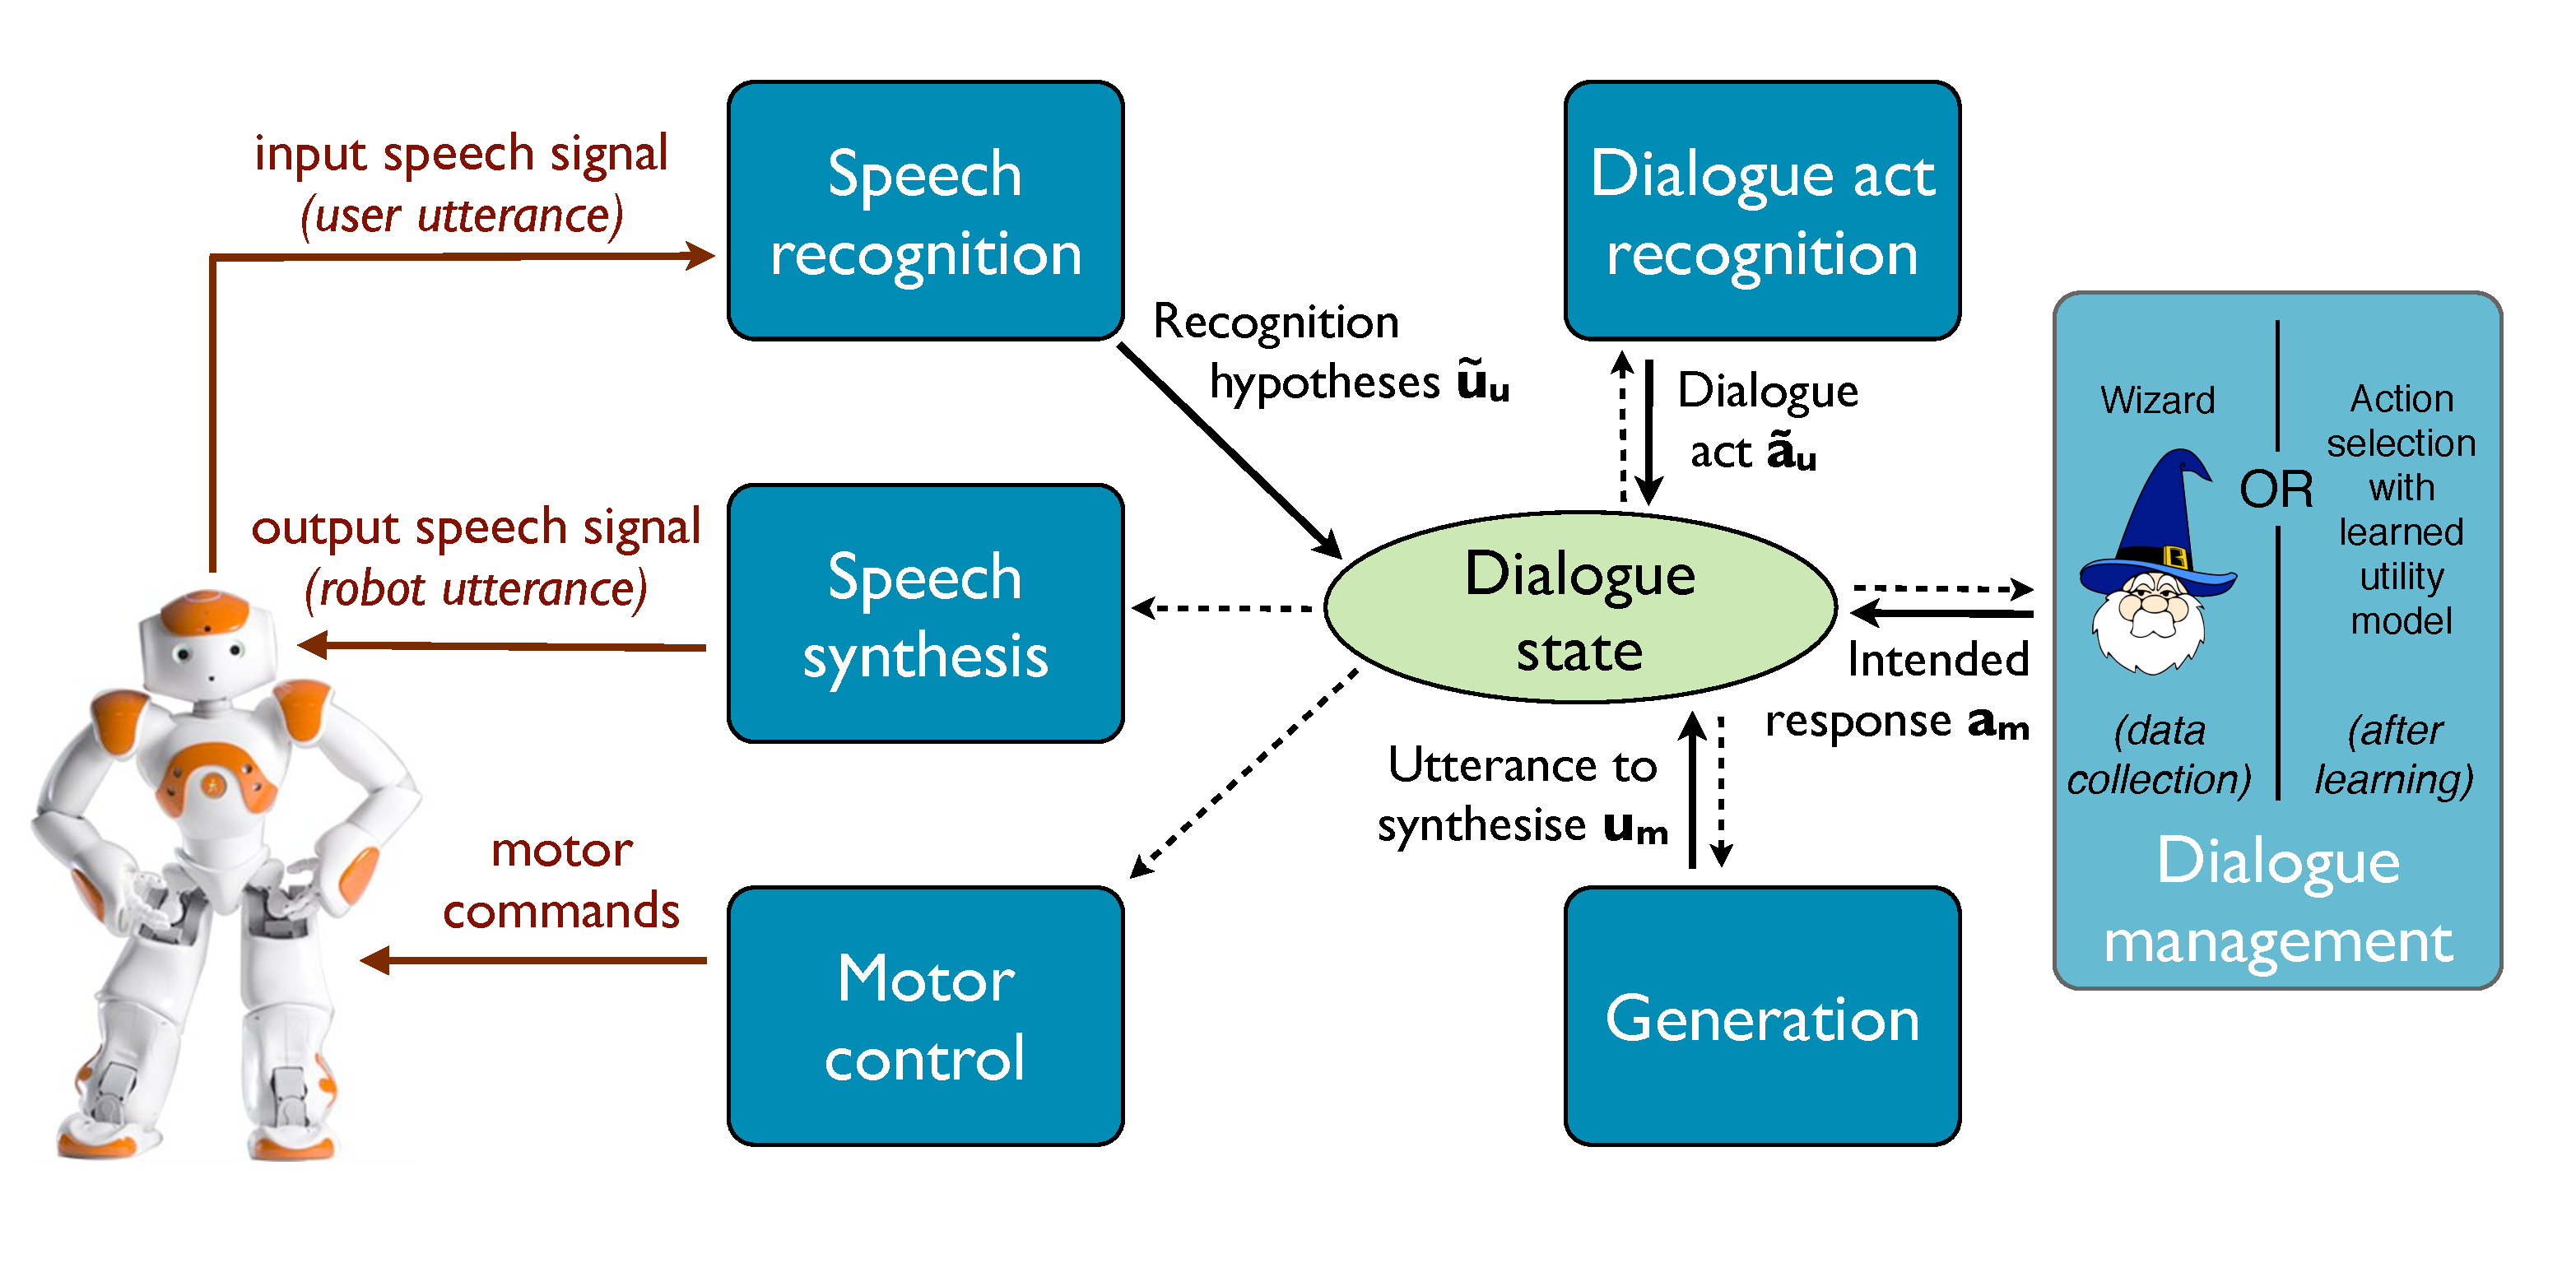
\includegraphics[scale=0.30]{imgs/exp1_architecture.pdf}
\end{center}
\caption{System architecture used for the experiment.}
\label{fig:exp1_architecture}
\end{figure}


The modules used for the experiments include in particular an off-the-shelf speech recogniser connected to four microphones placed on the robot head. The language model of the speech recogniser is encoded with a small hand-crafted recognition grammar, while the acoustic model was set to U.S. English. The corresponding user dialogue acts are then derived from the ASR hypotheses via a template-based recognition model. On the generation side, a shallow generation model is in charge of the surface realisation of the verbal actions which is then sent to the speech synthesis engine.  Finally, the execution of physical actions is delegated to a separate component, responsible for planning the robot movements and controlling its motors in real-time, based on the software libraries available on the robotic platform. 

\subsubsection*{Data collection procedure}
\index{Wizard-of-Oz interaction!data collection}
 Each recorded dialogue involved one human subject interacting with the Nao robot in a shared visual scene.  The dialogues were relatively short, with an average duration of about four minutes. We collected a total of 20 interactions with 7 distinct users, for a total of 1020 system turns, summing to around one hour of interaction.  The users were recruited amongst the students and researchers in the Department of Informatics at the University of Oslo, while the role of the wizard was taken by the author of the present thesis.  All the interactions were performed in English. All but one users were non-native speakers of English.\footnote{This mismatch between the acoustic model trained on native American speakers and the foreign accents of the participants may partly explain the relatively high level of speech recognition errors.}  As the speech recogniser relied on a language model of limited coverage, the users were briefed before each experiment about the comprehension capabilities of the robot in order to adjust their expectations about what the robot could and could not understand, and thereby limit the number of out-of-coverage utterances.

Wizard-of-Oz experiments should ideally place the wizard in the same types of decision contexts as the ones encountered by the dialogue manager. To this end, the wizard was prevented from listening directly to the spoken utterances of the user and was instead provided with the N-best list generated by the speech recogniser.  The N-best lists appeared on the wizard control screen as hypotheses accompanied with their respective probabilities. On the basis of these inputs, the wizard could then select the action to perform from a list of alternatives.  

Transcripts 1 and 2 present two recorded excerpts of Wizard-of-Oz interactions.  The user utterances are displayed as N-best lists of speech recognition hypotheses. 

\begin{Transcript}[p!]
\begin{dialogue} \vspace{3mm}
\speak{Human} $\begin{bmatrix}\text{ hello Lenny} & 0.22 \\
\text{ follow me} & 0.20 \\
\text{ hi Lenny} & 0.53 \end{bmatrix}$ \vspace{3mm}
\speak{Robot} \ \ \ Hello there!\vspace{3mm}
\speak{Human} $\begin{bmatrix}\text{ move your left arm up} & 0.41 \\
\text{ move the left arm up} & 0.27 \\
\text{ put your left arm up} & 0.30 \end{bmatrix}$ \vspace{3mm}
\speak{Robot} \ \ \ Sure! \vspace{2mm}\\
\direct{\refer{Robot} executes the movement $\mathrm{MoveArm(Left,Up)}$} \\
\direct{\refer{Robot} waits a few seconds} \vspace{2mm}
\speak{Robot} \ \ \ Was that correct? \vspace{3mm}
\speak{Human} $\begin{bmatrix}\text{ yes} & 0.88 \\
\text{ thanks} & 0.10 \end{bmatrix}$ \vspace{2mm} \\
\direct{\refer{Robot} registers the movement as confirmed} \vspace{3mm}
\speak{Robot} \ \ \ Great \vspace{3mm}
\speak{Human} $\begin{bmatrix}\text{ move your right arm up at the same time} & 0.26 \\
\text{ put the right arm up at the same time} & 0.32 \\
\text{  move the right arm up at the same time} & 0.38 \end{bmatrix}$ \vspace{3mm}
\speak{Robot} \ \ \ Let's see \vspace{1mm} \\
\direct{\refer{Robot} executes movement $\mathrm{MoveArm(Both,Up)}$} \vspace{2mm}
\speak{Robot} \ \ \ Was that correct? \vspace{3mm}
\speak{Human} $\begin{bmatrix}\text{ kneel} & 0.25 \\
\text{ thanks} & 0.14 \\
\text{  no} & 0.57 \end{bmatrix}$  \vspace{2mm} \\
\direct{\refer{Robot} discards last movement and goes back to previous position} \vspace{2mm}
\speak{Robot} \ \ \ What should I do then?  \\
\end{dialogue}
\vspace{-4mm} \hspace{1cm}\direct{...} \vspace{3mm}
\caption{User interaction with wizard-controlled robot, first excerpt}
\end{Transcript}

\begin{Transcript}[p!]
\vspace{4mm} \hspace{1cm} \direct{...}
\begin{dialogue} 
\speak{Human} $\begin{bmatrix}\text{ stop} & 0.25 \\
\text{ stand up} & 0.41 \\
\text{ no} & 0.25 \end{bmatrix}$ \vspace{3mm}
\speak{Robot} Let's see \vspace{1mm} \\
\direct{\refer{Robot} executes movement $\mathrm{StandUp}$} \vspace{3mm}
\speak{Human}  $\begin{bmatrix}\text{ put your right arm forward} & 0.31 \\
\text{ move your right arm forward} & 0.36 \\
\text{ move the right arm forward} & 0.30 \end{bmatrix}$ \vspace{2mm} \\
\direct{\refer{Robot} registers movement $\mathrm{StandUp}$ as implicitly confirmed} \vspace{2mm}
\speak{Robot} Let's see \vspace{1mm} \\
\direct{\refer{Robot} executes movement $\mathrm{MoveArm(Right,Forward)}$} \vspace{3mm}
\speak{Human} $\begin{bmatrix}\text{ move forward the left arm} & 0.31 \\
\text{ lower the left arm} & 0.35 \\
\text{ lower both arms} & 0.29 \end{bmatrix}$ \vspace{3mm}
\speak{Robot} Sorry, could you repeat? \vspace{3mm}
\speak{Human} $\begin{bmatrix}\text{ raise your left arm} & 0.28 \\
\text{ lift your right arm} & 0.31 \\
\text{ lift your left arm} & 0.37 \end{bmatrix}$ \vspace{3mm}
\speak{Robot} Sure \vspace{1mm} \\
\direct{\refer{Robot} executes movement $\mathrm{MoveArm(Left,Up)}$} \\
\direct{\refer{Robot} waits a few seconds} \vspace{3mm}
\speak{Robot} Should I do it like this? \\
\speak{Human} $\begin{bmatrix}\text{ kneel} & 0.23 \\
\text{ wrong} & 0.22 \\
\text{ no} & 0.47 \end{bmatrix}$ \vspace{3mm} \\
\direct{\refer{Robot} discards last movement and goes back to previous position} \vspace{2mm}
\speak{Robot} What should I do then?  \vspace{3mm}
\speak{Human} $\begin{bmatrix}\text{ move your left arm up} & 0.29 \\
\text{ move the left arm up} & 0.34 \\
\text{ move the left arm down} & 0.28 \end{bmatrix}$ \vspace{3mm} \\
\end{dialogue}
\vspace{-4mm} \hspace{1cm} \direct{...} \vspace{3mm}
\caption{User interaction with wizard-controlled robot, second excerpt}
\end{Transcript}

\subsubsection*{Dialogue state}
\index{dialogue state}
Each selected action $a_m$ was recorded along with the complete dialogue state $\mathcal{B}$ in effect at the time of the selection. The dialogue state consisted of five independent variables: \begin{enumerate}
\item The last user dialogue act $a_u$ (with the values given in Table \ref{table:userdas})
\item The last system action $a_m$ (with the values given in Table \ref{table:systemdas})
\item The recorded sequence of (confirmed) movements, encoded as a list (cf. Section \ref{sec:amodelling})
\item The last physical movement demonstrated by the robot
\item Finally, a periodically updated variable expressing the number of seconds elapsed since the last user or system action.  This variable is used to determine when the system should ask for an explicit confirmation from the user.
\end{enumerate}

The state variables are represented with their full probability distributions. The dialogue state recorded right before the wizard registers the first movement in Transcript 1 corresponds for instance to the following specification: 
\begin{align*}
\mathcal{B} = \begin{cases} a_u = [ (\mathrm{Confirm}, p\!=\!0.88), (\mathrm{Say(ThankYou)}, p\!=\!0.10), (\mathit{None}, p\!=\!0.02) \rangle \\
a_m = \langle (\mathrm{AskConfirmation}, p\!=\!1) ] \\
\mathit{moveSequence} = [ ( \emptyset, p\!=\!1) ] \\
\mathit{lastMove} = [ (\mathrm{MoveArm(Left,Up)}, p\!=\!1) ] \\
\mathit{silence} = [ (0 \textrm{ seconds}, p\!=\!1) ] \end{cases}
\end{align*}

\subsection{Experimental setup}
\label{sec:wozlearning-experiments-setup}

The central question investigated in this experiment is the following: Does the encoding of dialogue management models in terms of probabilistic rules improve the efficiency of the parameter estimation process compared to more traditional representations? If yes, how significant is the difference? The experiment focused therefore on the learning performance of various utility models based on limited amounts of training data gathered from Wizard-of-Oz interactions. The parameters correspond here to the utilities of the various system actions depending on the current state.

\subsubsection*{Baseline models}

The experiment relied on two distinct baselines that express the utility model of the domain based on traditional representations: \begin{enumerate}
\item The first baseline is a plain utility table\index{utility table} that maps every combination of state values and actions to a particular utility.  For a given set of state variables $X_1, \dots, X_n$, 
the utility for the system action $a_m$ is therefore defined by: 
\begin{equation}
U(X_1=x_1, \dots, X_n=x_n, a_m) = \theta_{(x_1, \dots, x_n, a_m)}
\end{equation}
where the $\theta_{(x_1, \dots, x_n, a_m)}$ value corresponds to the utility encoded in the table for the state--action pair. The number of required parameters is thus $|\mathit{Val}(X_1)| \times \dots \times |\mathit{Val}(X_n)| \times |\mathit{Val}(a_m)|$. In order to keep the model tractable, the utility table was factored in the experiments in three parts, each responsible for a subset of the possible system actions. These utility tables comprised a total of 8962 independent parameters. 
%\begin{align*}
%&U(a_u,a_m,\mathit{lastMove},\mathit{moveSequence},\mathit{silence},a_{m}') \\ 
%&= U(a_u, a_m,a_{m}') + U(a_u,\mathit{lastMove},a_{m}') + U(a_m,\mathit{silence},a_{m}') 
%\end{align*}
\item The second baseline defines the utility of a given action as a linear combination\index{linear model} of values -- one for each state variable.  The total utility is thus determined as:
\begin{equation}
U(X_1=x_1, \dots, X_n=x_n, a_m) = \sum_{i=1}^{n} \theta_{(x_i, a_m)}
\end{equation}
where $\theta_{(x_i, a_m)}$ corresponds to the utility weight of the variable value $x_i$ for the action $a_m$.  Note that the weights are specific to a given action value. The number of required parameters is here $|\mathit{Val}(a_m)| \times (|\mathit{Val}(X_1)| + \dots + |\mathit{Val}(X_n)|)$.  As a consequence, the size of the linear model is reduced to 581 independent parameters.  However, this baseline hinges on the assumption that the total utility of a given action can be decomposed as a linear combination of weights for each state variable value.
\end{enumerate}

\subsubsection*{Rule-structured model}
\index{rule-structured model}
The two baselines were compared to a utility model structured with 15 utility rules. The interested reader is invited to browse the specification of these rules in Appendix \ref{chap:domainspecs}. The rule structure was designed by hand, while the parameters (in this case, utility values) remained unknown. The rules were associated to a total of 24 parameters. 

\subsubsection*{Parameter estimation}
\index{parameter estimation}

Figure \ref{fig:exp1_baselines} offers a graphical comparison of the utility models produced for the two baselines and the rule-structured approach.  The two baselines are essentially ``flattened'' or unstructured versions of the rule-based model.  The input and output variables remain identical in all three models. However, the two baselines directly associate each state--action combination to a single utility value, while the rule-structured approach defines this overall utility in a more indirect manner, through the instantiation of multiple utility rules. 

\begin{figure}[ht]
\centering
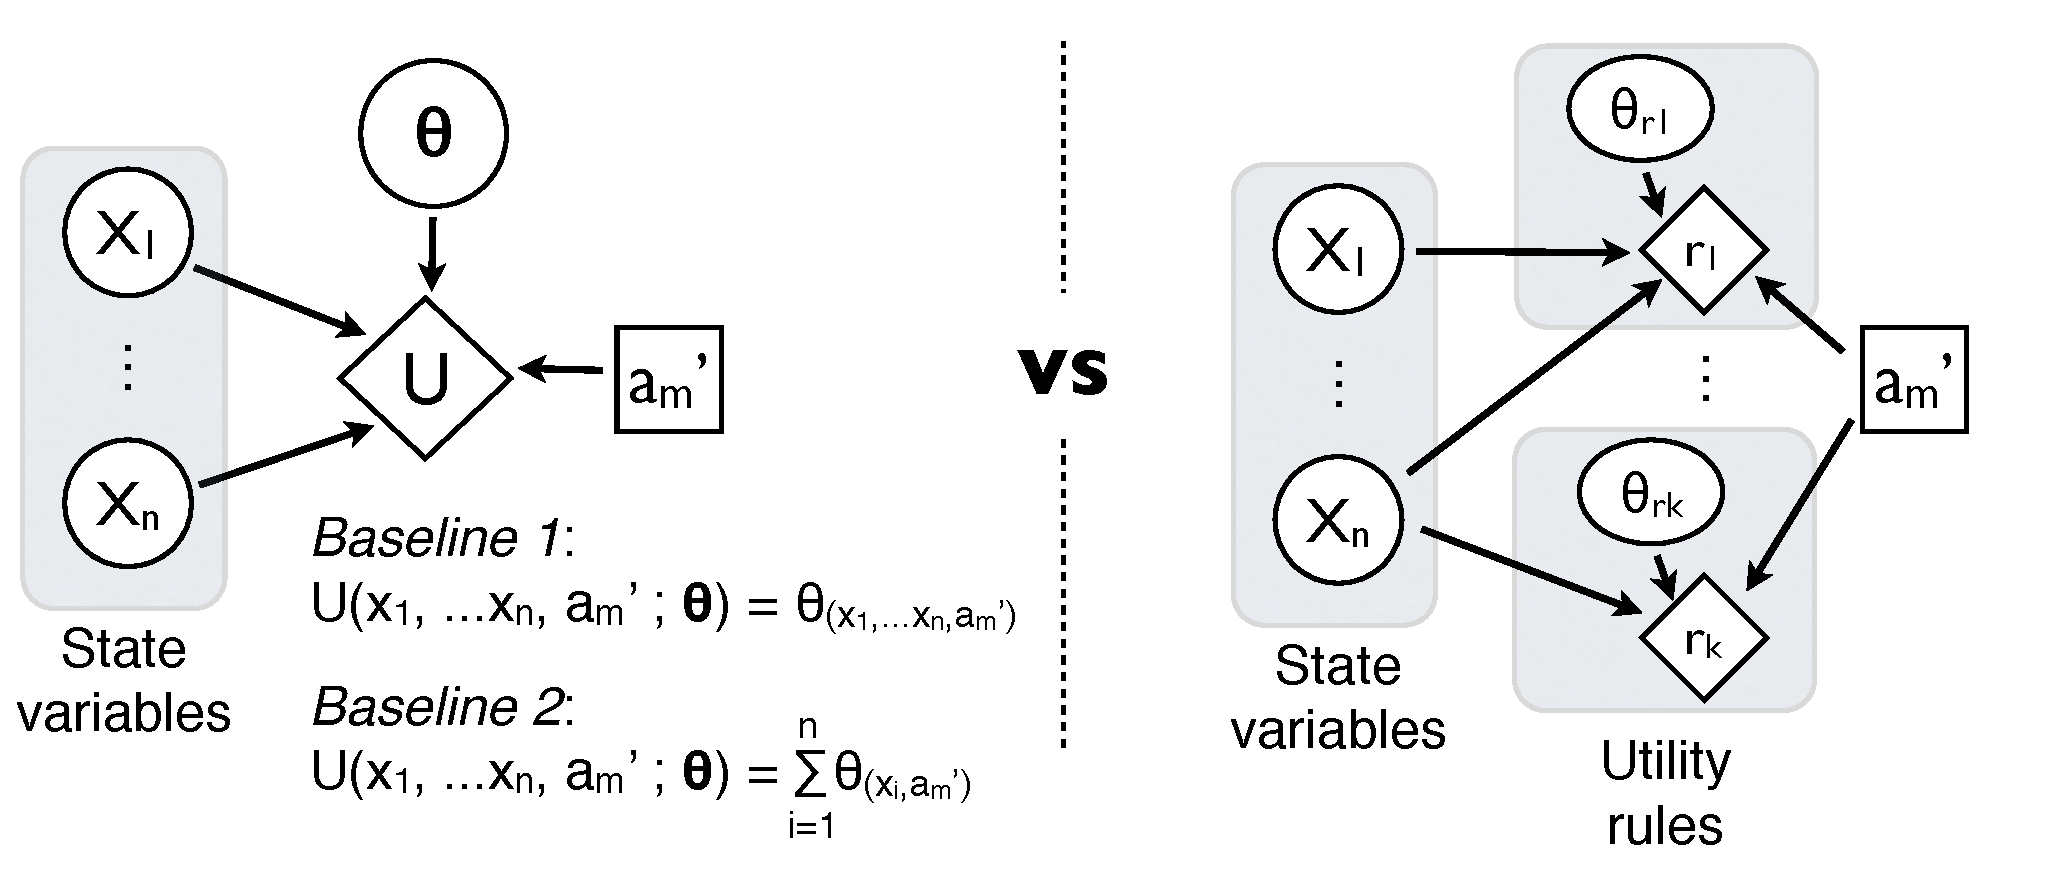
\includegraphics[scale=0.40]{imgs/exp1_baselines.pdf}
\caption{Baseline utility models (left) compared to the rule-structured utility model (right).}
\label{fig:exp1_baselines}
\end{figure}


The parameter estimation procedure followed the Bayesian learning approach detailed in Section \ref{sec:rule-supervised-learning}.  The prior distributions on the utility values were initialised with uniform priors on the interval $[-1,6]$ in all three models. 

%For the baseline models, the function \textsc{triggerModels}(...) resulted in the creation of one single utility node connected to the system action, as illustrated in Figure \ref{fig:exp1_baselines}.

\subsubsection*{Evaluation of learning performance}
\index{learning performance}
Given the utility models defined above, the selected action simply corresponds to the action associated with the maximum utility in the current state. In this particular experiment, utility maximisation only considered the current (immediate) utility and did not perform forward planning.

The data collected from the Wizard-of-Oz interactions was split into a training set composed of 765 state--action pairs (75 \% of the gathered data) and a held-out test set with 255 actions (remaining 25 \%). The same training set was used to estimate the utility parameters for the three models.  The resulting utility models were then evaluated on the basis of their agreement with the wizard actions in the held-out test set. This agreement is determined to be the proportion of system-selected actions that are identical to the action chosen by the wizard. The agreement results for the three models were evaluated at various stages of the estimation process in order to analyse and compare their learning performance. The results were practically calculated by sampling over the parameters, performing inference over the resulting models, and finally averaging over the inference results.  

\subsection{Empirical results and analysis}
\label{sec:wozlearning-experiments-results}

Table \ref{table} presents the agreement results for the three utility models. The differences between the rule-structured model and the two baselines are statistically significant using Bonferroni-corrected paired $t$-tests, with $p$-value $< 0.0001$.   

We performed an error analysis on the 17\% of actions that deviate from the wizard behaviour.\footnote{One should be wary of labelling these actions as ``incorrect'', since they are in most cases relevant dialogue moves, but simply result from slightly different decision strategies than the one followed by the wizard.} The analysis revealed that the discrepancy is mainly due to two factors.  The first factor is the lack of complete consistency on the part of the wizard, who occasionally decided to follow distinct strategies in similar situations (especially regarding the use of clarification requests). The second factor is the presence of a non-negligible number of spurious and noisy data points, notably caused by interruptions and technical issues with the robotic platform (e.g.\ movements that had to be repeated due to motor failures).

\begin{table}[ht]
\begin{center}
\begin{tabular}{|l|c|} \hline
\textit{Type of model} & \textit{Agreement (in \%) } \\ \hline \hline
Plain utility table & 67.35 \\ \hline
Linear model & 61.85 \\ \hline
Rule-structured model & \textbf{82.82} \\ \hline
\end{tabular}
\end{center}
\vspace{-2mm}
\caption{Agreement results for the three models on a held-out test set.}
\vspace{-2mm}
\label{table}
\end{table}

The learning curves for the three models are shown in Figure \ref{results}\index{learning curve}.   Note that since the parameters are initially uniformly distributed, the agreement is already non-zero before learning, since a random assignment of parameters has a low but non-zero chance of leading to the right action. 


\begin{figure*}[p!]
\begin{center}\subfigure[Linear scale]{
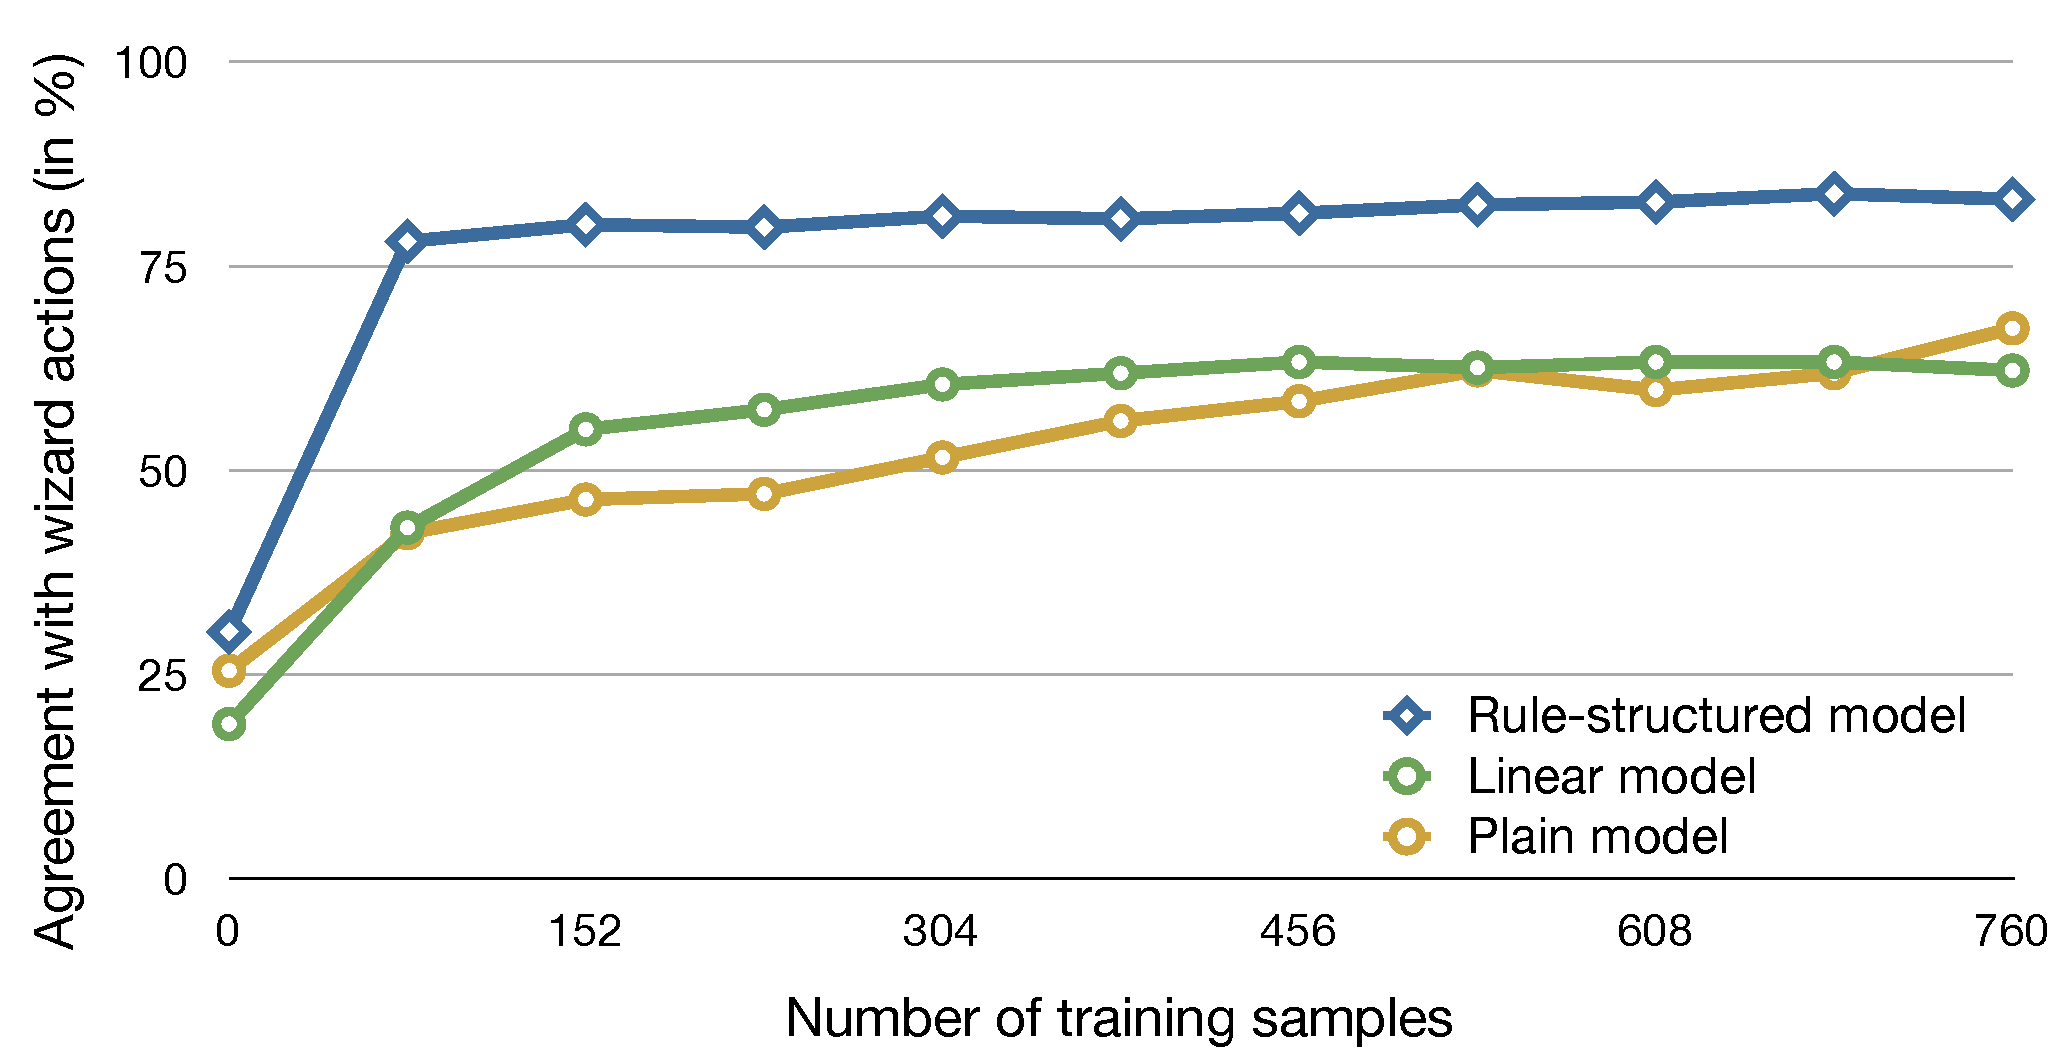
\includegraphics[scale=0.38]{imgs/results_linear.pdf}
}\end{center} $\phantom{a}$\vspace{8mm}$\phantom{a}$ 
\begin{center}\subfigure[Logarithmic scale (base 2)]{
\centering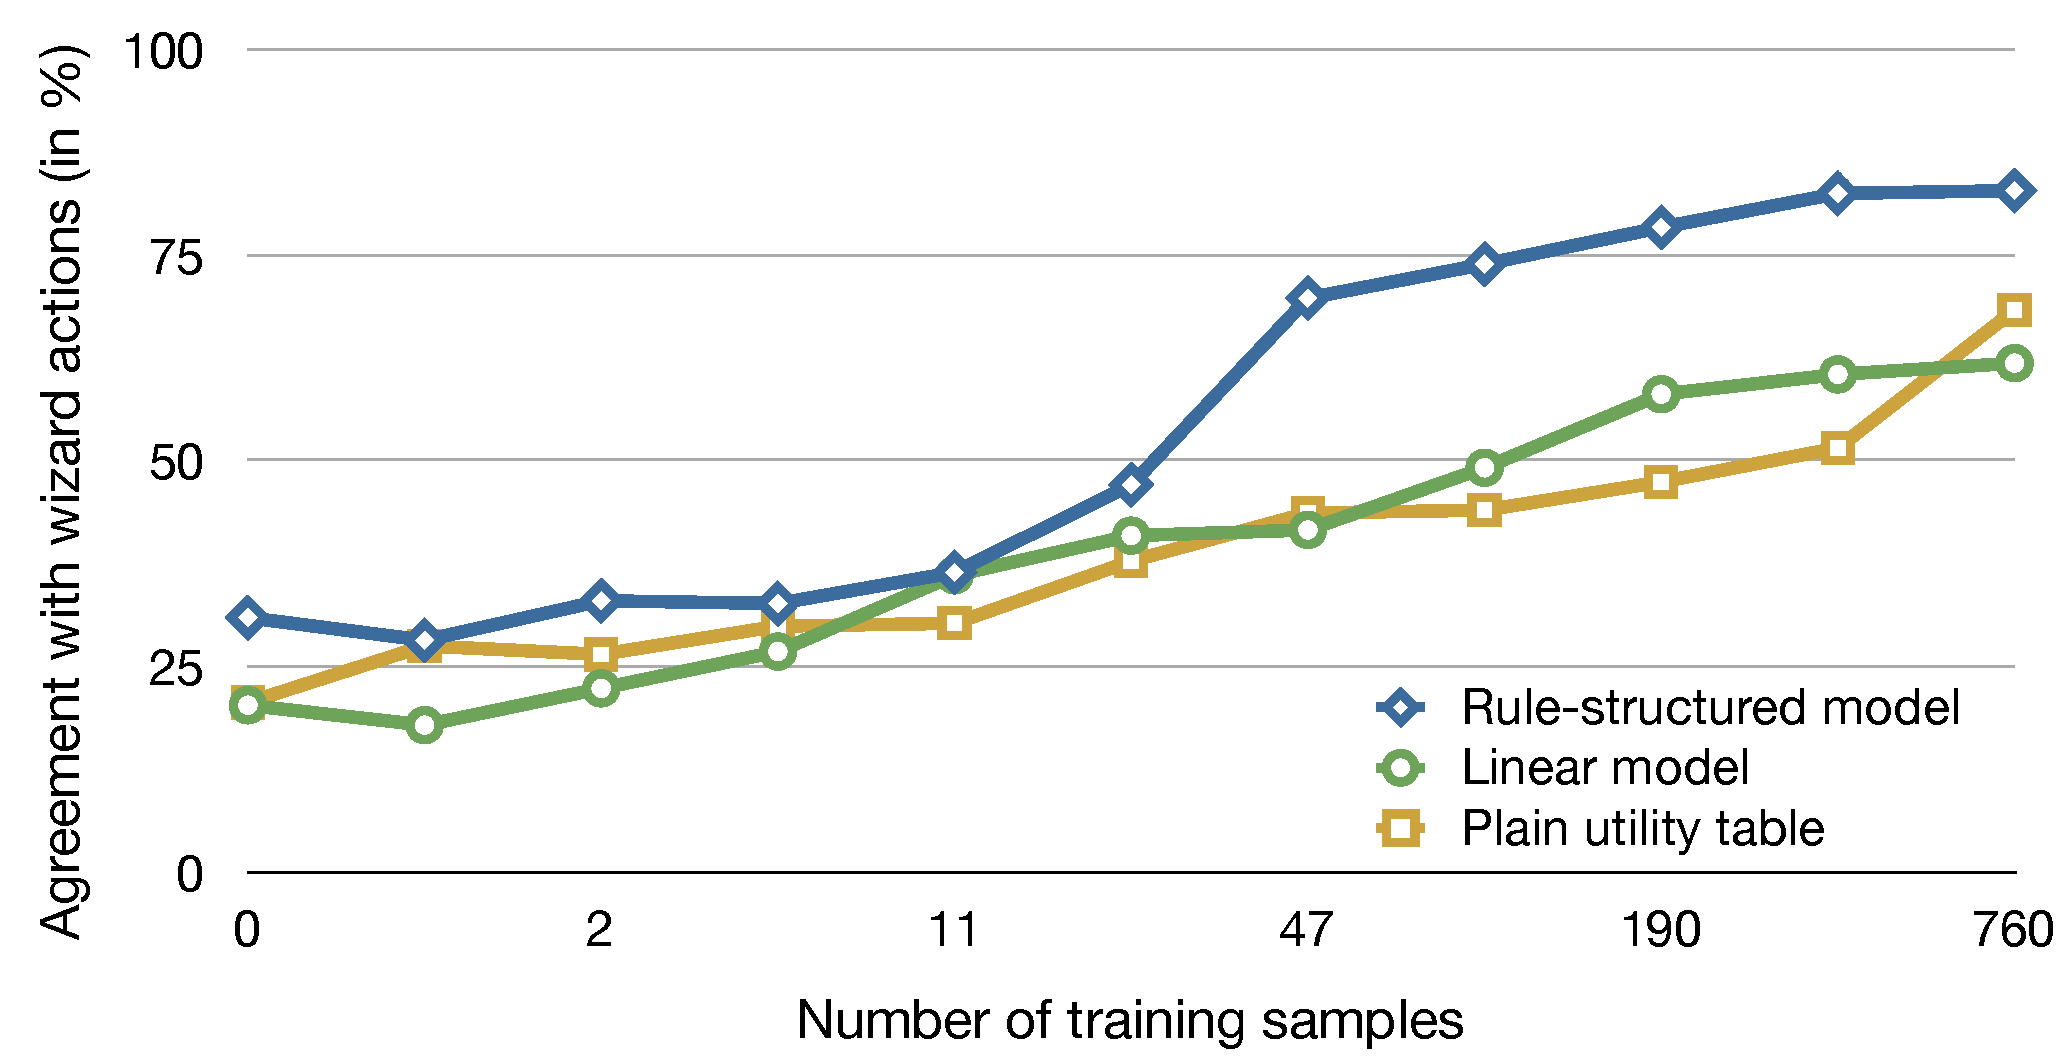
\includegraphics[scale=0.38]{imgs/results_log.pdf}
}\end{center}
\caption{Learning curves for the three utility models on the test set as a function of the number of processed data points.  The agreement results are given for the plain, linear and rule-structured utility models, using both linear (top) and logarithmic scales (bottom).}
\label{results}
\end{figure*}


Thanks to its considerably reduced number of parameters, the rule-structured model is able to converge to near-optimal values after observing only a small fraction of the training set.  The incorporation of domain knowledge via the rule structure has a clearly beneficial effect on the learning performance and on the generalisation capacity of the model\index{generalisation capacity}.  As the figure shows, the two baseline models do also improve their accuracies over time, but at a much slower rate.   The linear model is comparatively faster than the plain model, but levels off towards the end. The suboptimal learning performance of the linear model is most likely due to the non-linearity of some dialogue strategies.  The plain model continues its convergence and would probably reach an agreement level similar to the rule-structured model if given much larger amounts of training data. 

The learning results are in line with our expectations based on the respective sizes of the parameter space for the three utility models, and are not \textit{per se} highly surprising.  The main lesson to draw from this experiment is, however, not the exact difference in agreement or learning rates for each particular model, but the fact that probabilistic rules can be successfully applied to structure a small but non-trivial dialogue domain and derive its parameters from collected interaction data.  Through the use of abstraction mechanisms such as partitioning and quantification, the experiment demonstrates that the utility rules specified for the domain can cover large regions of the problem space without degrading the accuracy of the model.  The utility model can hence be optimised with only modest amounts of in-domain data. 


\section{Conclusion}
\label{sec:woz-conclusions}

The present chapter has described how parameters could be included in the specification of probabilistic rules and estimated via Bayesian learning techniques.  Rule parameters can represent either probability or utility values. The estimation process operates by calculating posterior probability distributions over possible parameter values given the observed data set. The process is initiated with prior distributions such as Dirichlet priors for probability values and Gaussian or uniform priors for utilities. 

The main focus of the chapter was on supervised learning of rule parameters based on Wizard-of-Oz training data. We described how Wizard-of-Oz data can be practically collected and processed to yield data points encoded as pairs <dialogue state $\mathcal{B}_i$, wizard action $a_i$>.  
These data points are used to progressively narrow down the spread of the posterior distributions to the values that provide the best fit for the observed wizard actions. 

This learning approach has been implemented in a spoken dialogue system for human--robot interaction and validated in a proof-of-concept experiment.  The goal of the experiment was to estimate the utility values of various actions on the basis of a Wizard-of-Oz data set.  Three utility models were compared: a plain utility table, a linear model, and a model structured with utility rules. The analysis of the empirical results shows that the rule-structured model outperforms the two baselines in regards to learning rate and generalisation performance. 

The outcome of the experiment corroborates one of the central claims of this thesis -- namely, that hybrid approaches to dialogue modelling (and in particular the formalism of probabilistic rules presented in this thesis) are well suited to model dialogue domains that must simultaneously confront high levels of uncertainty and limited availability of in-domain dialogue data. In such situations, which are commonplace in the field of spoken dialogue systems, neither purely symbolic nor purely data-driven approaches are alone sufficient to harness the complex and stochastic nature of the interactions.  Hybrid approaches provide ways to combine expert knowledge and statistically optimised parameters in a single, unified framework, thereby allowing dialogue models to be tuned from even small amounts of training data. 

As shown in the experiments, Wizard-of-Oz interaction data can be a useful and interesting source of domain knowledge for the estimation of probabilistic models of dialogue. The data collection procedure can, however, be a tedious endeavour, as it requires:
\begin{enumerate}
\item The availability of an expert (the wizard) that can control the system and provide examples of appropriate behaviour for the domain.
\item The technical setup of a Wizard-of-Oz environment from which the wizard can perceive the user inputs, monitor contextual features, select possible actions to execute, and get all relevant information recorded and stored in a generic format. 
\end{enumerate}

A natural alternative to supervised learning from Wizard-of-Oz data is to let the dialogue system learn the best conversational behaviour via trial and error from its own interaction experience (that is, through reinforcement learning), without relying on the provision of external examples.\index{reinforcement learning}  The next chapter demonstrates how such a strategy can be practically implemented, based once again on the formalism of probabilistic rules to structure the domain models. 


\chapter{Learning from interactions}
\label{chap:rllearning}
This chapter extends the parameter estimation approach developed in the previous chapter to a reinforcement learning context.  As explained in the first part of this thesis, a reinforcement learning agent learns how to act through a process of trial and error in a given environment.  In our case, the environment is represented by verbal interactions with human users, and the system behaviour to learn corresponds to dialogue policies mapping dialogue states to relevant system responses. 

The optimisation process is in many respects similar to the one already outlined. Bayesian inference remains the basic instrument for updating distributions over the model parameters on account of the collected evidence.  However, the evidence is no longer represented by examples of expert behaviour as in supervised learning. The learning agent instead actively gathers experience through repeated interactions with (real or simulated) users, and receives feedback on its actions in the form of new observations and rewards. The parameter distributions are gradually refined on the basis of this feedback and subsequently employed to select the next actions to execute. The use of probabilistic rules\index{probabilistic rule} allows the learning agent to  escape the ``curse of dimensionality''\index{curse of dimensionality} that often characterises dialogue domains. As a consequence, the number of interactions required to reach dialogue policies of high quality can be greatly reduced. 

The chapter is divided in three sections.  After a short survey of the core concepts of Bayesian reinforcement learning in Section \ref{sec:brl}, we expose in Section \ref{sec:rl-ruleparams} our own reinforcement learning approach to the estimation of rule parameters.  More specifically, we present how the parameters of probabilistic rules can be automatically optimised from interactions using either model-based or model-free strategies. Finally, Section \ref{sec:rllearning-experiments} reports on a learning experiment carried out in a human--robot interaction domain. The purpose of the experiment was to analyse the performance of rule-structured models compared to standard categorical distributions. Empirical results on a user simulator show that the rule-structured models converge to optimal parameters -- and hence achieve higher returns -- in a much shorter time than unstructured representations. 

\section{Bayesian reinforcement learning}\index{Bayesian reinforcement learning|textbf}
\label{sec:brl}

Bayesian reinforcement learning has recently emerged as a generic framework for learning and acting in uncertain environments \citep{poupart2008,Ross:2011,brl2012}. As in other types of Bayesian learning methods, the core idea of Bayesian reinforcement learning is to maintain explicit probability distributions over the domain parameters and gradually narrow down the spread of these distributions as more experience is collected. However, in contrast to supervised approaches, the learning agent is no longer a mere passive observer in the interaction, as it must actively decide how to act after each turn in order to move the interaction forward. 

As explained in Section \ref{sec:rl}, the actions selected by the agent must strike a balance between exploration (trying out new actions) and exploitation (preferring actions that are most likely to yield higher rewards). Bayesian reinforcement learning can offer principled solutions to the exploration--exploitation dilemma\index{exploration--exploitation dilemma}, as model uncertainty is explicitly accounted for in the action selection process \citep{Duff:2002,Ross:2011}.  A Bayesian agent will therefore select actions that are expected to provide the highest long-term return given the current model uncertainty. When the uncertainty is high, information-gathering actions are preferred since they lead to a better understanding of the environment dynamics and are therefore more likely to result in higher future rewards. This inclination to explore gradually fades away as the learning agent develops a better grasp of its domain and becomes more confident about the relative merits of its own actions.
%\footnote{The representation of this model uncertainty and its inclusion in the action selection process can however take multiple forms \cite[see e.g.][for more details]{brl2012}.}

As for other families of reinforcement learning methods, Bayesian reinforcement learning can be divided in model-based and model-free methods. 


\subsubsection*{Model-based methods}
\index{Bayesian reinforcement learning!model-based methods for}

Model-based methods estimate an explicit model of the domain in the form of transition, observation and reward models.  One advantage of model-based approaches is the relative simplicity of parameter estimation, as the model parameters can be directly updated upon the reception of each observation and reward using standard Bayesian inference. The policy is, however, complex to optimise, due to the combination of three types of uncertainty: state uncertainty, stochastic action effects, and model uncertainty. The result is an augmented POMDP where the state also includes random variables expressing the model parameters in addition to traditional state variables \citep{Duff:2002,Ross:2011}. 

For domains of small to medium size, approximate dynamic programming\index{dynamic programming} methods can be applied to generate the $\boldsymbol\alpha$-vectors for this augmented POMDP.  Point-based solvers \citep{Porta:2006,shani2013} have notably demonstrated reasonable performance on a variety of problems. These solution methods are, however, difficult to scale to more complex models due to the computational intractability of the optimisation process.    

An alternative to offline approaches is online planning\index{online planning}.  Instead of compiling a policy for all possible states (as done in dynamic programming), online planning concentrates on selecting the best action for the current state at runtime. This selection is typically implemented through the construction of a lookahead search tree representing possible actions and their effects in terms of rewards and new observations. This tree is gradually expanded until a particular planning horizon is reached.  Several approximate methods have recently been developed, based on e.g.\ point-based value iterations \citep{ross2008} and Monte Carlo tree search \citep{NIPS2010_0740}. The action leading to the highest return on the search tree is then executed by the agent.  

One important benefit of online approaches is the possibility to dynamically adapt the domain models at runtime. This characteristic is useful for dialogue domains where the domain models can vary in the course of the interaction -- for instance, in order to adapt to shifting user preferences. Offline approaches must in comparison recalculate their policies after every modification or extension of the internal models for the domain.   However, this advantage comes at a price, namely the fact that planning must be performed at execution time, while the interaction is taking place.  Planning must therefore meet real-time constraints. 

Interestingly, offline and online approaches are not mutually exclusive, but can be combined together to take full advantage of both strategies.  The idea is to perform offline planning to precompute an initial rough policy, and use this policy as a heuristic approximation to guide the search of an online planner \citep{RossC07}. These heuristic approximations can for instance be used to provide lower and upper bounds on the values associated with the dialogue states of the search tree.  Based on these bounds, the planning algorithm can concentrate its computational efforts in the most fruitful regions of the search space and quickly discard irrelevant actions. 

Model-based Bayesian reinforcement learning has been applied to dialogue management in several recent papers.  \cite{DBLP:journals/jstsp/PngPC12} describe a generic Bayes-Adaptive POMDP\index{Bayes-Adaptive POMDP} framework and illustrate its use in simulated interactions. \cite{DoshiR08} present a similar POMDP framework with model uncertainty combined with active learning.  Action selection is formalised in their paper by sampling possible POMDP models and extracting a solution for each sample. A related strategy is employed in a less principled manner by \cite{DBLP:conf/iui/AtrashP09}.  Finally, \cite{ChinaeiC12} and \cite{chinaei2012} demonstrate the estimation of observation and reward models for dialogue POMDPs in an healthcare application.  One interesting aspect of their work is the use of inverse reinforcement learning to automatically derive a reward model from expert policies.

\subsubsection*{Model-free methods}
\index{Bayesian reinforcement learning!model-free methods for}

Model-free methods adopt a different learning strategy and directly optimise a dialogue policy from experience, without attempting to construct explicit internal models of the domain. One simple method, first formalised by \ \cite{Dearden:1998}, is to assign prior distributions to the $Q$ value estimates associated with state--action pairs, and iteratively refine these distributions upon the completion of each action. This update generally relies on Bellman's equation\index{Bellman's equation}, since the $Q$ values are never directly observed (only the observations and rewards are available to the agent). The optimal action is then simply defined as the one that maximises the $Q$ values for the current state, modulo an ``exploration bonus'' added at learning time to favour exploratory strategies.  

Gaussian processes\index{Gaussian processes} can be used to extend model-free approaches to problems with continuous state and action spaces \citep{Engel:2005}. Policy gradient methods that optimise a parametrised policy by gradient ascent are also popular \citep{GhavamzadehE06}. 

%Other Bayesian model-free approaches rely on Gaussian processes, which extend the above approach to problems with continuous state and actions spaces , and policy gradient methods, which directly optimise a parametrised policy by gradient ascent \citep{GhavamzadehE06}.  

%Policy gradient methods have also been combined with actor-critic methods to reduce the variance of the parameter estimates \citep{Ghavamzadeh:2007}.

\cite{milica2013} present a framework for dialogue policy optimisation based on Gaussian processes. One of the main benefits of their approach is the tremendous acceleration of the optimisation procedure.  As a result, the dialogue policy can be optimised via live interactions with human users instead of being confined to simulation. \cite{Supelec808} describe a related approach based on Kalman Temporal Differences\index{Kalman Temporal Differences}.  As their approach is grounded in Kalman filtering instead of full Bayesian filtering, it only estimates the first and second moment of the parameter distributions -- i.e.\ its mean and variance -- instead of the full posterior distributions, as explained in \cite{DBLP:journals/jair/GeistP10}. 

Finally, it is worth nothing that Bayesian reinforcement learning has also been applied to partially observable dialogue domains which necessitate the estimation of a transition model to update the dialogue state, even though the dialogue policy itself is optimised in a model-free manner \citep{DBLP:conf/slt/ThomsonJGKMYY10}. 


\subsubsection*{Scalability}

Bayesian reinforcement learning has been the subject of much recent research in the last decade, based on both model-based and model-free paradigms. This research focus led to the development of powerful optimisation methods \cite[see e.g.][for a detailed survey]{brl2012}. Nevertheless, scalability remains an important concern when porting these methods to real applications, as the sizes of the parameter and action spaces can  constitute major bottlenecks for many learning methods, especially in partially observable domains. 

As argued in the next section, probabilistic rules\index{probabilistic rule} can contribute to addressing this issue by reducing the number of parameters and filtering out irrelevant actions from the planning process.

\section{Optimisation of rule parameters}
\label{sec:rl-ruleparams}
\index{rule parameters!reinforcement learning of}

This thesis develops two distinct approaches to the optimisation of rule parameters from unannotated interactions. Both employ Bayesian reinforcement learning as theoretical framework and probabilistic rules as representation formalism, but follow distinct optimisation strategies:

\begin{itemize}
\item The first approach follows a model-based strategy.  In this approach, the rule-structured models $\mathcal{M}$ of the domain correspond to transition, observation and reward models. The models are associated with a collection of parameters $\boldsymbol\theta$ with prior distributions $P(\boldsymbol\theta)$.  These parameter distributions are updated on the basis of the observations and rewards received by the system during the interactions. Forward planning is employed at runtime to calculate the expected cumulative utilities of possible actions and select the one yielding the maximum utility given the current dialogue state and rule parameters. 

\item The second approach is a model-free strategy relying on parametrised utility rules representing the estimated $Q$ value for the system actions. In contrast to the model-based strategy, the utility parameters are here updated via a temporal-difference learning method.  The actions to execute are determined through an $\epsilon$-greedy policy that strikes a balance between the selection of known high-utility actions and the exploration of new actions.

\end{itemize}

The two sections below flesh out these two approaches in more detail. 

\subsection{Model-based approach}
\label{sec:modelbased}
\index{rule parameters!model-based RL of}

The model-based approach relies on the specification of probabilistic rules that capture:\index{probabilistic rule}
\begin{itemize}
\item the \textit{transition model} for the domain, which describes how the dialogue state is likely to change as a result of the system actions\index{transition model},
\item the \textit{observation model} for the domain, which describes the likely observations associated with a given dialogue state\index{observation model},
\item the \textit{reward model} for the domain, which describes the immediate rewards (reflecting the system objectives) that result from the execution of particular system actions\index{reward model}.
\end{itemize}

Figure \ref{fig:modelbasediagram} depicts a dynamic decision network\index{dynamic decision network} corresponding to the above definition. The transition model is encoded as a probability distribution $P(s_t \, | \, s_{t-1}, a_{t-1} \,; \boldsymbol\theta_T)$, the observation model by a probability distribution $P(o_t \, | \, s_t\,; \boldsymbol\theta_O)$ and the reward model by the utility distribution $R_t(s_t,a_t\,; \boldsymbol\theta_R)$. For the sake of clarity, the figure abstracts away from the rule nodes mediating between the variables in the network, and upon which the parameters are attached.

\begin{figure}[ht]
\centering
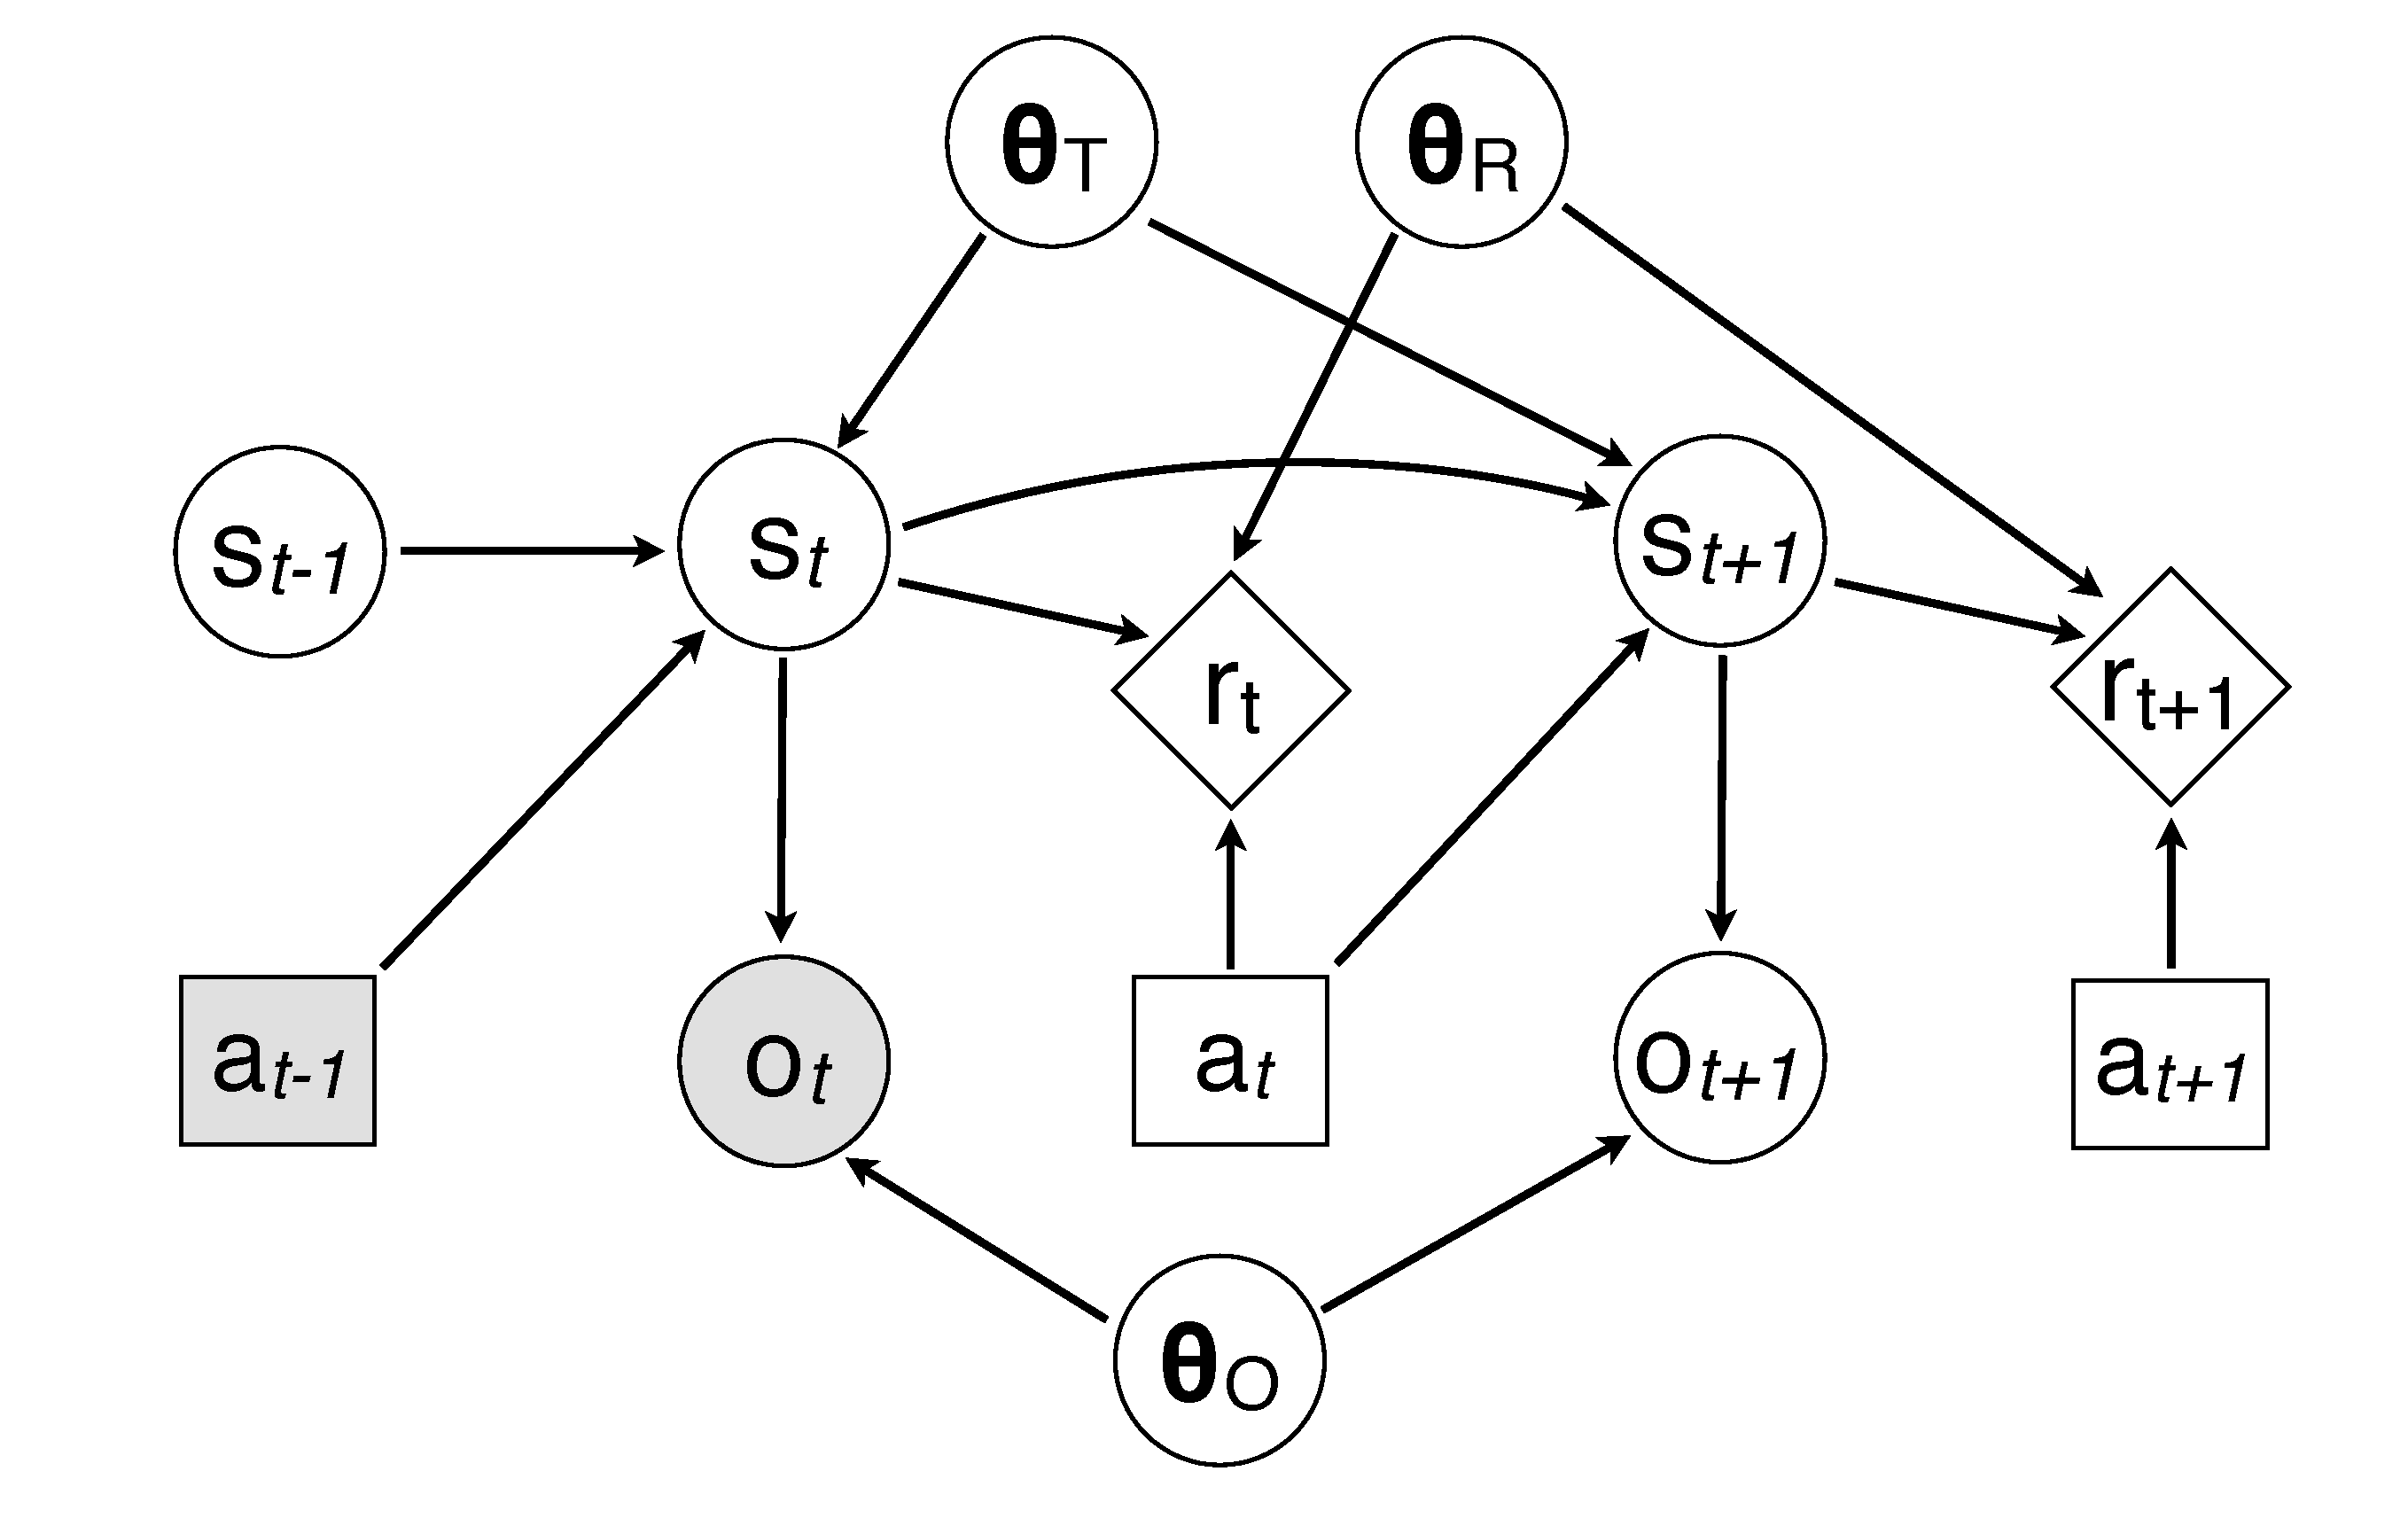
\includegraphics[scale=0.25]{imgs/modelbaseddiagram.pdf}
\caption{Dynamic decision network for a model-based learning strategy.}
\label{fig:modelbasediagram}
\end{figure}

\subsubsection*{Parameter estimation}
\index{parameter estimation}
The probabilistic rules corresponding to these three models may all include unknown parameters that must be estimated from data.  Fortunately, this worst case scenario where $\boldsymbol\theta_T$, $\boldsymbol\theta_R$ and $\boldsymbol\theta_O$ must all be learned from scratch rarely happens in practice. As evidenced in the experiment described at the end of this chapter, the reward and observation models can indeed often be defined by the system designer prior to learning. 
%The transition model is typically the domain model that is most difficult to capture, as it expresses the dynamics of the interaction -- i.e.\ how the user is expected to interact with the system. 

Two types of information sources are available to the agent to refine its parameters during the interaction: the observations and the rewards.  In the model-based setting, parameter update is relatively straightforward.  The key idea is to include the parameter variables as part of the dialogue state.  The probability distributions of these parameters are automatically updated as part of the state update process (see Algorithm \ref{algo:stateupdate} in Section \ref{sec:processing-workflow}). There is therefore no need for special purpose mechanisms beyond standard Bayesian inference.\index{Bayesian learning}

\subsubsection*{Example of parameter update}

Let us illustrate this process on the domain example from Section \ref{sec:detailedexample}, if we assume the effect distribution associated with the predictive rule $r_{11}$ to be unknown and replaced by parameters: 
\begin{align*}
r_{11}: \ \ & \forall y, \\ 
& \textbf{if} \ (a_m = \mathit{AskRepeat} \land a_u=y) \ \textbf{then} \\ 
& \; \;  \begin{cases} 
P(a_{u\mbox{-}p} = y) = \theta_{r_{11}(1,1)} \\ 
P(\{\cdot\}) = \theta_{r_{11}(1,2)} \\ 
\end{cases}
\end{align*}


Figure \ref{fig:learningexample} illustrates how the distribution over the parameter values for $\boldsymbol\theta_{r_{11}(1)}$ is automatically modified as part of the state update operation.  The dialogue example remains unchanged:
\begin{dialogue} 
\speak{User } Now move forward \\ $\phantom{b}$ $\tilde{a}_u = [ (\mathit{Request(Forward)}, 0.6), (\mathit{Request(Backward)}), 0.4)]$  \\[-3mm]
\speak{System } Could you please repeat? \\[-3mm]
\speak{User } Please move forward! \\ $\phantom{b}$ $\tilde{a}_u = [ (\mathit{Request(Forward)}, 0.7), (\mathit{Other}, 0.2), (\mathit{Request(Backward)}, 0.1) ]$ \\[-4mm]
\end{dialogue} 

To keep the example as simple as possible, the figure ignores the steps related to action selection and concentrates on the application of rule $r_{11}$.  The initial distribution $P(\boldsymbol\theta_{r_{11}(1)})$ is set in this example to $\sim \mathrm{Dirichlet}(2,1)$, as we can reasonably presuppose that the users are more likely than not to repeat their last utterance after an explicit request from the system.

\begin{figure}[ht]
\centering
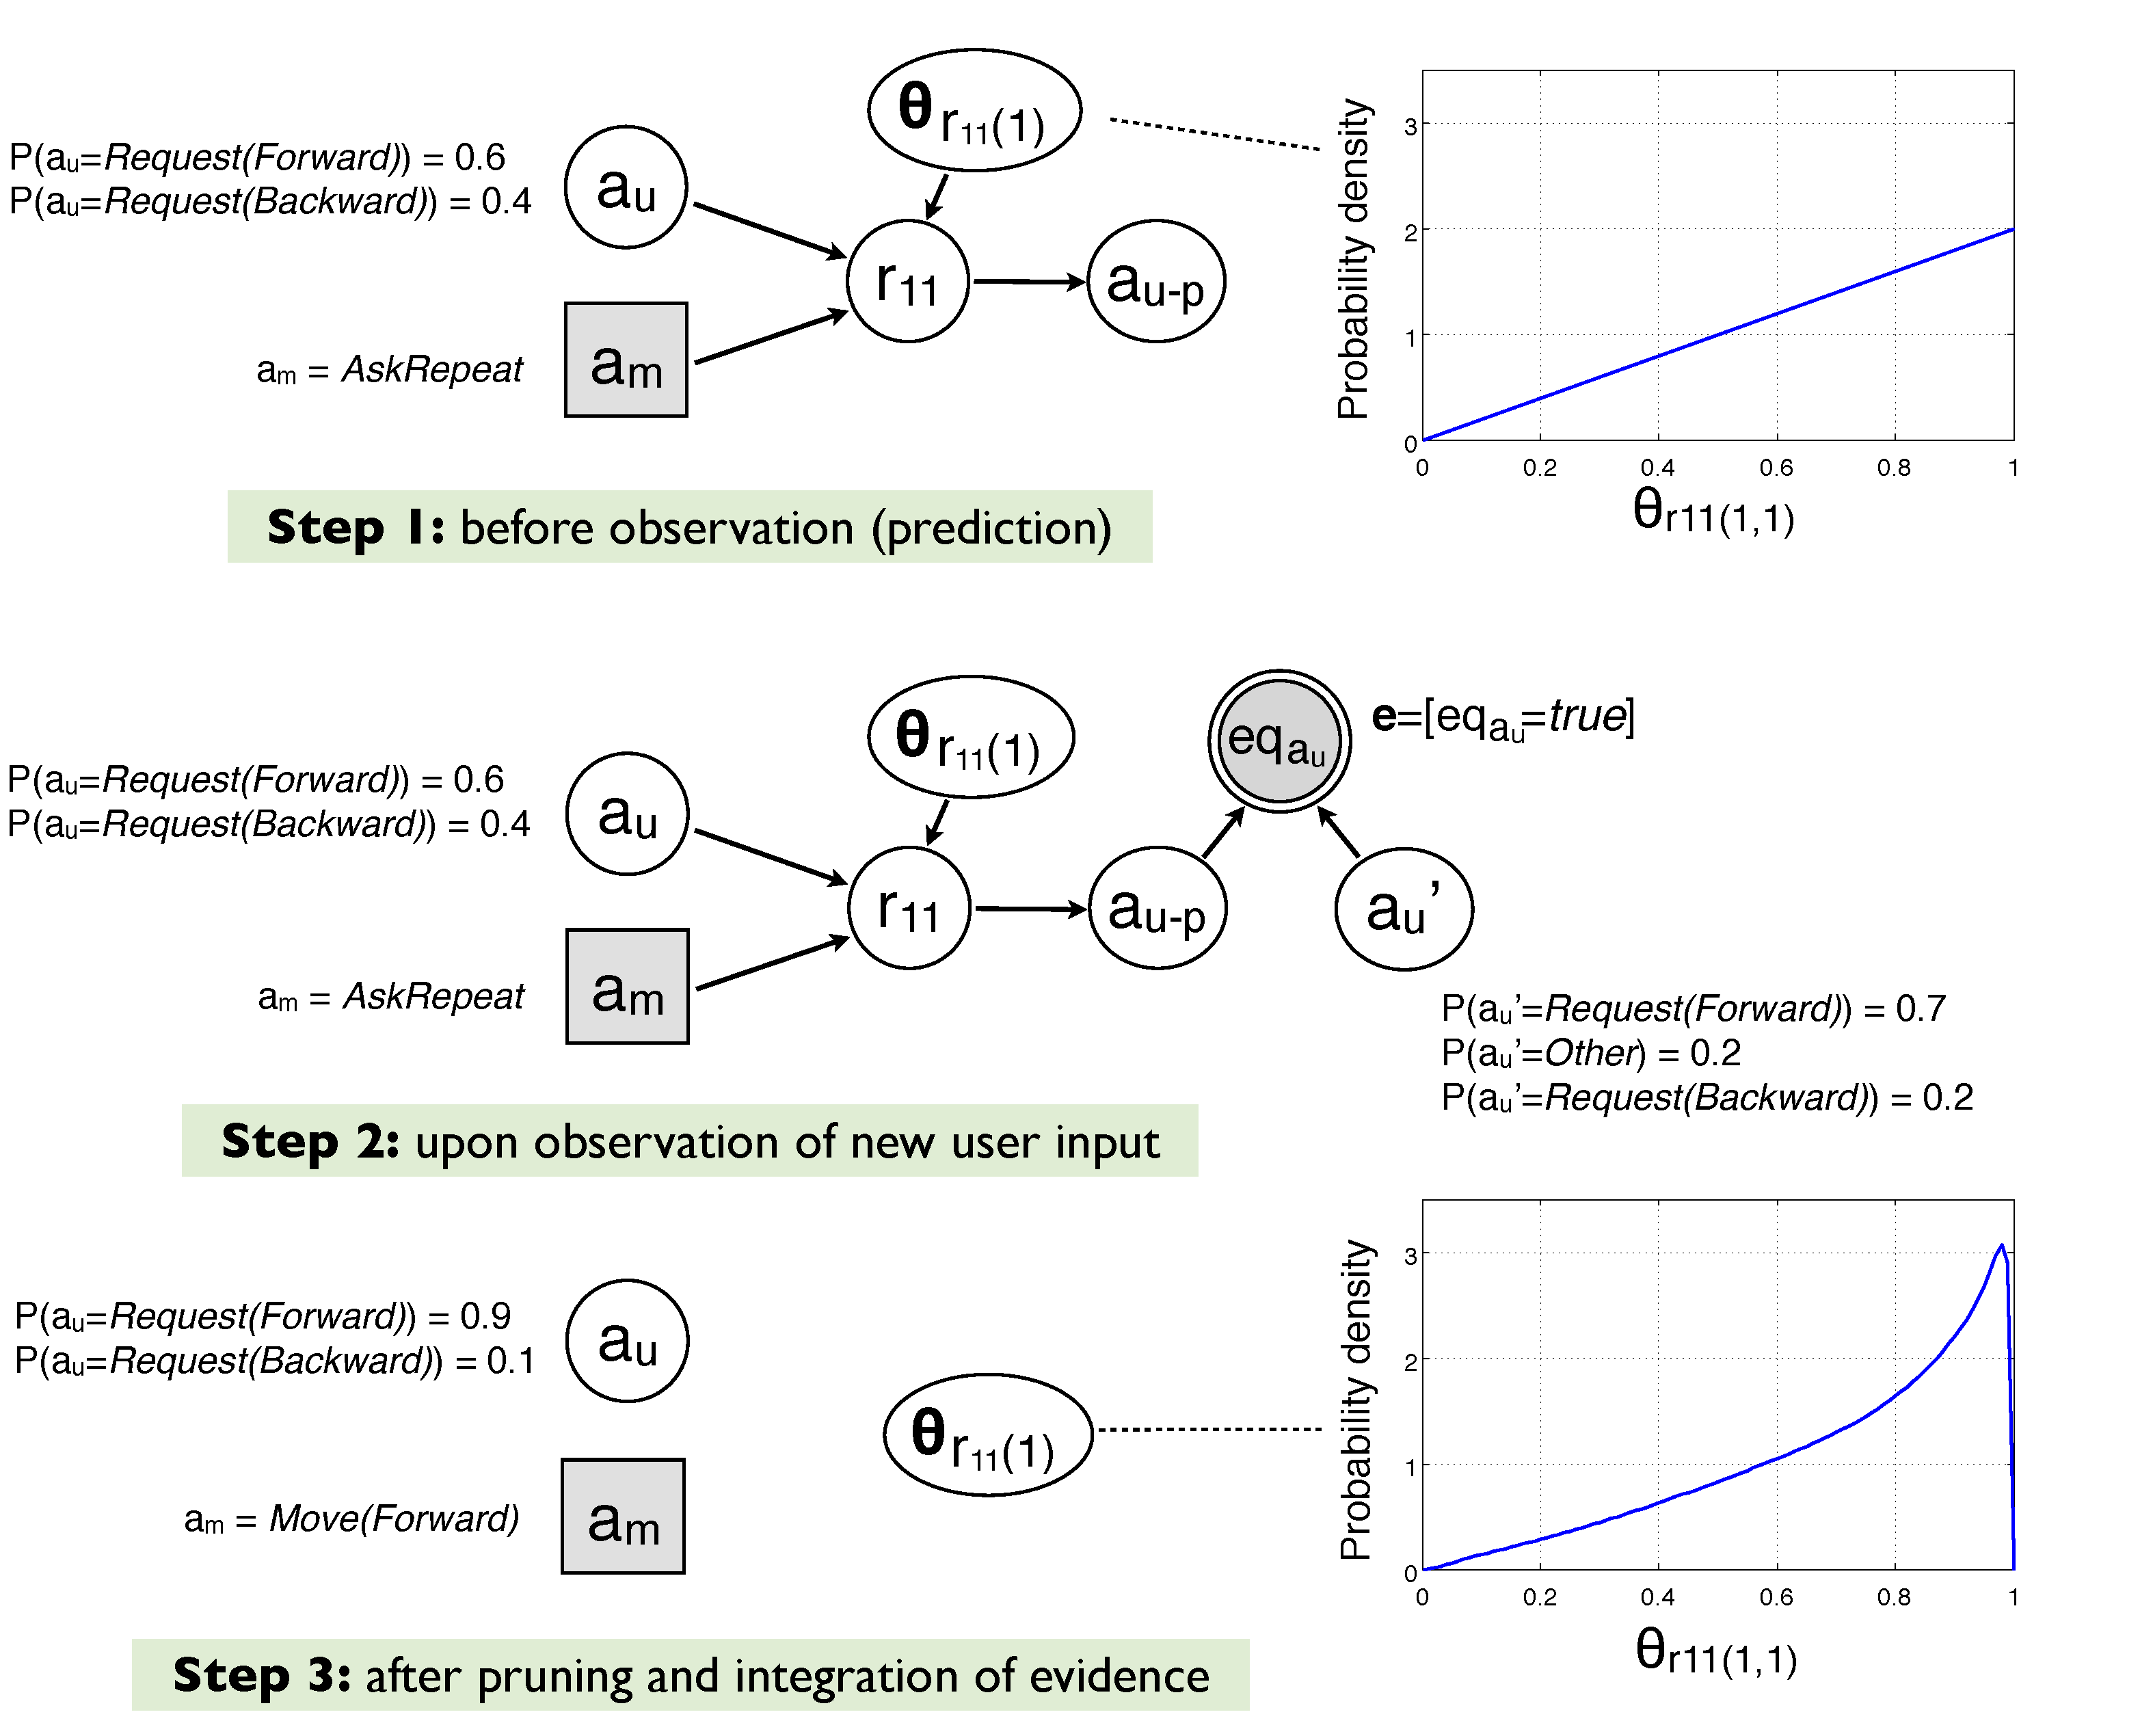
\includegraphics[scale=0.30]{imgs/learningexample.pdf}
\caption{Parameter update for $\boldsymbol\theta_{r_{11}(1)}$ after the reception of a new user input. }
\label{fig:learningexample}
\end{figure}

The first step illustrates the instantiation of the rule along with its parameter. Upon the reception of a new observation in the form of a user input $a_u'$, the dialogue state and parameters are updated (step 2). After pruning and integration of the evidence (step 3), we notice that the parameter distribution $P(\boldsymbol\theta_{r_{11}(1)})$ has shifted part of its probability mass further to the right. In other words, the probability of the users repeating their last utterance becomes somewhat more likely. The posterior distribution\index{posterior parameter distribution} $P(\boldsymbol\theta_{r_{11}(1)})$ after the update is constructed using kernel density estimation. 

\subsubsection*{Action selection}
\index{action selection}

 As the $Q$ values are not directly accessible in model-based approaches, action selection must resort to either dynamic programming or forward planning to calculate the expected future rewards of each action.  Action selection is the computational bottleneck in model-based Bayesian reinforcement learning, since the agent needs to reason not only over all the current and future states, but also over all possible models (parametrised by the $\boldsymbol\theta$ variables).  The high dimensionality of the task often prevents the use of offline solution techniques. We apply in this work a simple forward planning algorithm coupled with importance sampling. \index{online planning}\index{planning horizon}

Algorithm \ref{algo:planning} selects the action to execute through forward planning on a given horizon $h$.  The selection procedure relies on the recursive function \textsc{Calculate-Q-Values}($\mathcal{B}, \mathbf{e}, h$) to compute the Q-values of possible actions given a current state $\mathcal{B}$, evidence $\mathbf{e}$ and planning horizon $h$.  

\begin{algorithm}[h!]
\caption{: \textsc{PlanAction} ($\mathcal{B}, \mathbf{e}$, h) }
\begin{algorithmic}[1] \vspace{1mm}
\REQUIRE Dialogue state $\mathcal{B}$ as a decision network
\REQUIRE Evidence $\mathbf{e}$
\REQUIRE Planning horizon $h$
\ENSURE Selected action $\mathbf{a}^*$
\STATE $Q_{\mathcal{B}} \leftarrow $ \textsc{Calculate-Q-Values} ($\mathcal{B}, \mathbf{e}, h)$
\STATE Find optimal value $\mathbf{a}^* = \argmax_{\mathbf{a}} Q_{\mathcal{B}}(\mathbf{a})$
\STATE Remove utility nodes from the state $\mathcal{B}$
\RETURN $\mathbf{a}^*$
\end{algorithmic}
\label{algo:planning}
\end{algorithm}


\begin{algorithm}[h!]
\caption{: \textsc{Calculate-Q-Values} ($\mathcal{B}, \mathbf{e}, h)$}
\begin{algorithmic}[1] \vspace{1mm}
\STATE Let $\mathbf{A}$ be the set of all decision variables in $\mathcal{B}$
\FORALL {possible action $\mathbf{a} \in \mathit{Val}(\mathbf{A})$}
\STATE $Q_{\mathcal{B}}(\mathbf{a}) \leftarrow U_{\mathcal{B}}(\mathbf{a}, \mathbf{e})$
\IF {$h > 1$}
\STATE $\mathcal{B}' \leftarrow $ dialogue state updated from $\mathcal{B}$ after action $\mathbf{a}$
\FORALL {possible observation $\mathbf{o}$}
\STATE $\mathcal{B} \leftarrow $ dialogue state updated from $\mathcal{B}'$ after observation $o$
\STATE $Q_{\mathcal{B}''} \leftarrow $ \textsc{Calculate-Q-Values}($\mathcal{B}'', \mathbf{e}, h -1$)
\STATE $Q_{\mathcal{B}}(\mathbf{a}) \leftarrow Q_{\mathcal{B}}(\mathbf{a}) + \gamma \ P_{\mathcal{B}'}(\mathbf{o}) \ \max_{\mathbf{a}'} Q_{\mathcal{B}''}(\mathbf{a}')$
\ENDFOR
\ENDIF
\ENDFOR
\RETURN $Q_{\mathcal{B}}$
\end{algorithmic} 
\label{algo:qval}
\end{algorithm}

The $Q$ value of an action is the discounted sum of its immediate reward (line 3 in Algorithm \ref{algo:qval}) and the expected future reward following its execution (line 4-11).  Line 6 loops on possible observations.  For efficiency reasons, only a limited number of high-probability observations are selected. For each observation, the dialogue state is updated (line 7) and the $Q$ values for the resulting state $\mathcal{B}''$ are computed (line 8).  The maximum $Q$ value for this future state is then added to the $Q$ value for the current state, weighted by the discount factor $\gamma$ and the probability $P_{\mathcal{B}'} (\mathbf{o})$ of the observation.  The procedure stops when the planning horizon has been reached, or the algorithm has run out of time. The planner then simply selects the action with maximum expected cumulative utility. 

Algorithm \ref{algo:qval} contains two loops: one cycling over the set of possible actions, and one cycling over the set of possible observations following the system action. This process can be represented in an AND-OR search tree anchored in the current state.\index{AND-OR search tree} The OR branches denote the system actions along with their respective rewards, while the AND branches denote the observations weighted by their likelihood. An example of such AND-OR search tree is provided in Figure \ref{fig:modelbasediagram}, which is modified from \cite{ross2008}.


\begin{figure}[h!]
\centering
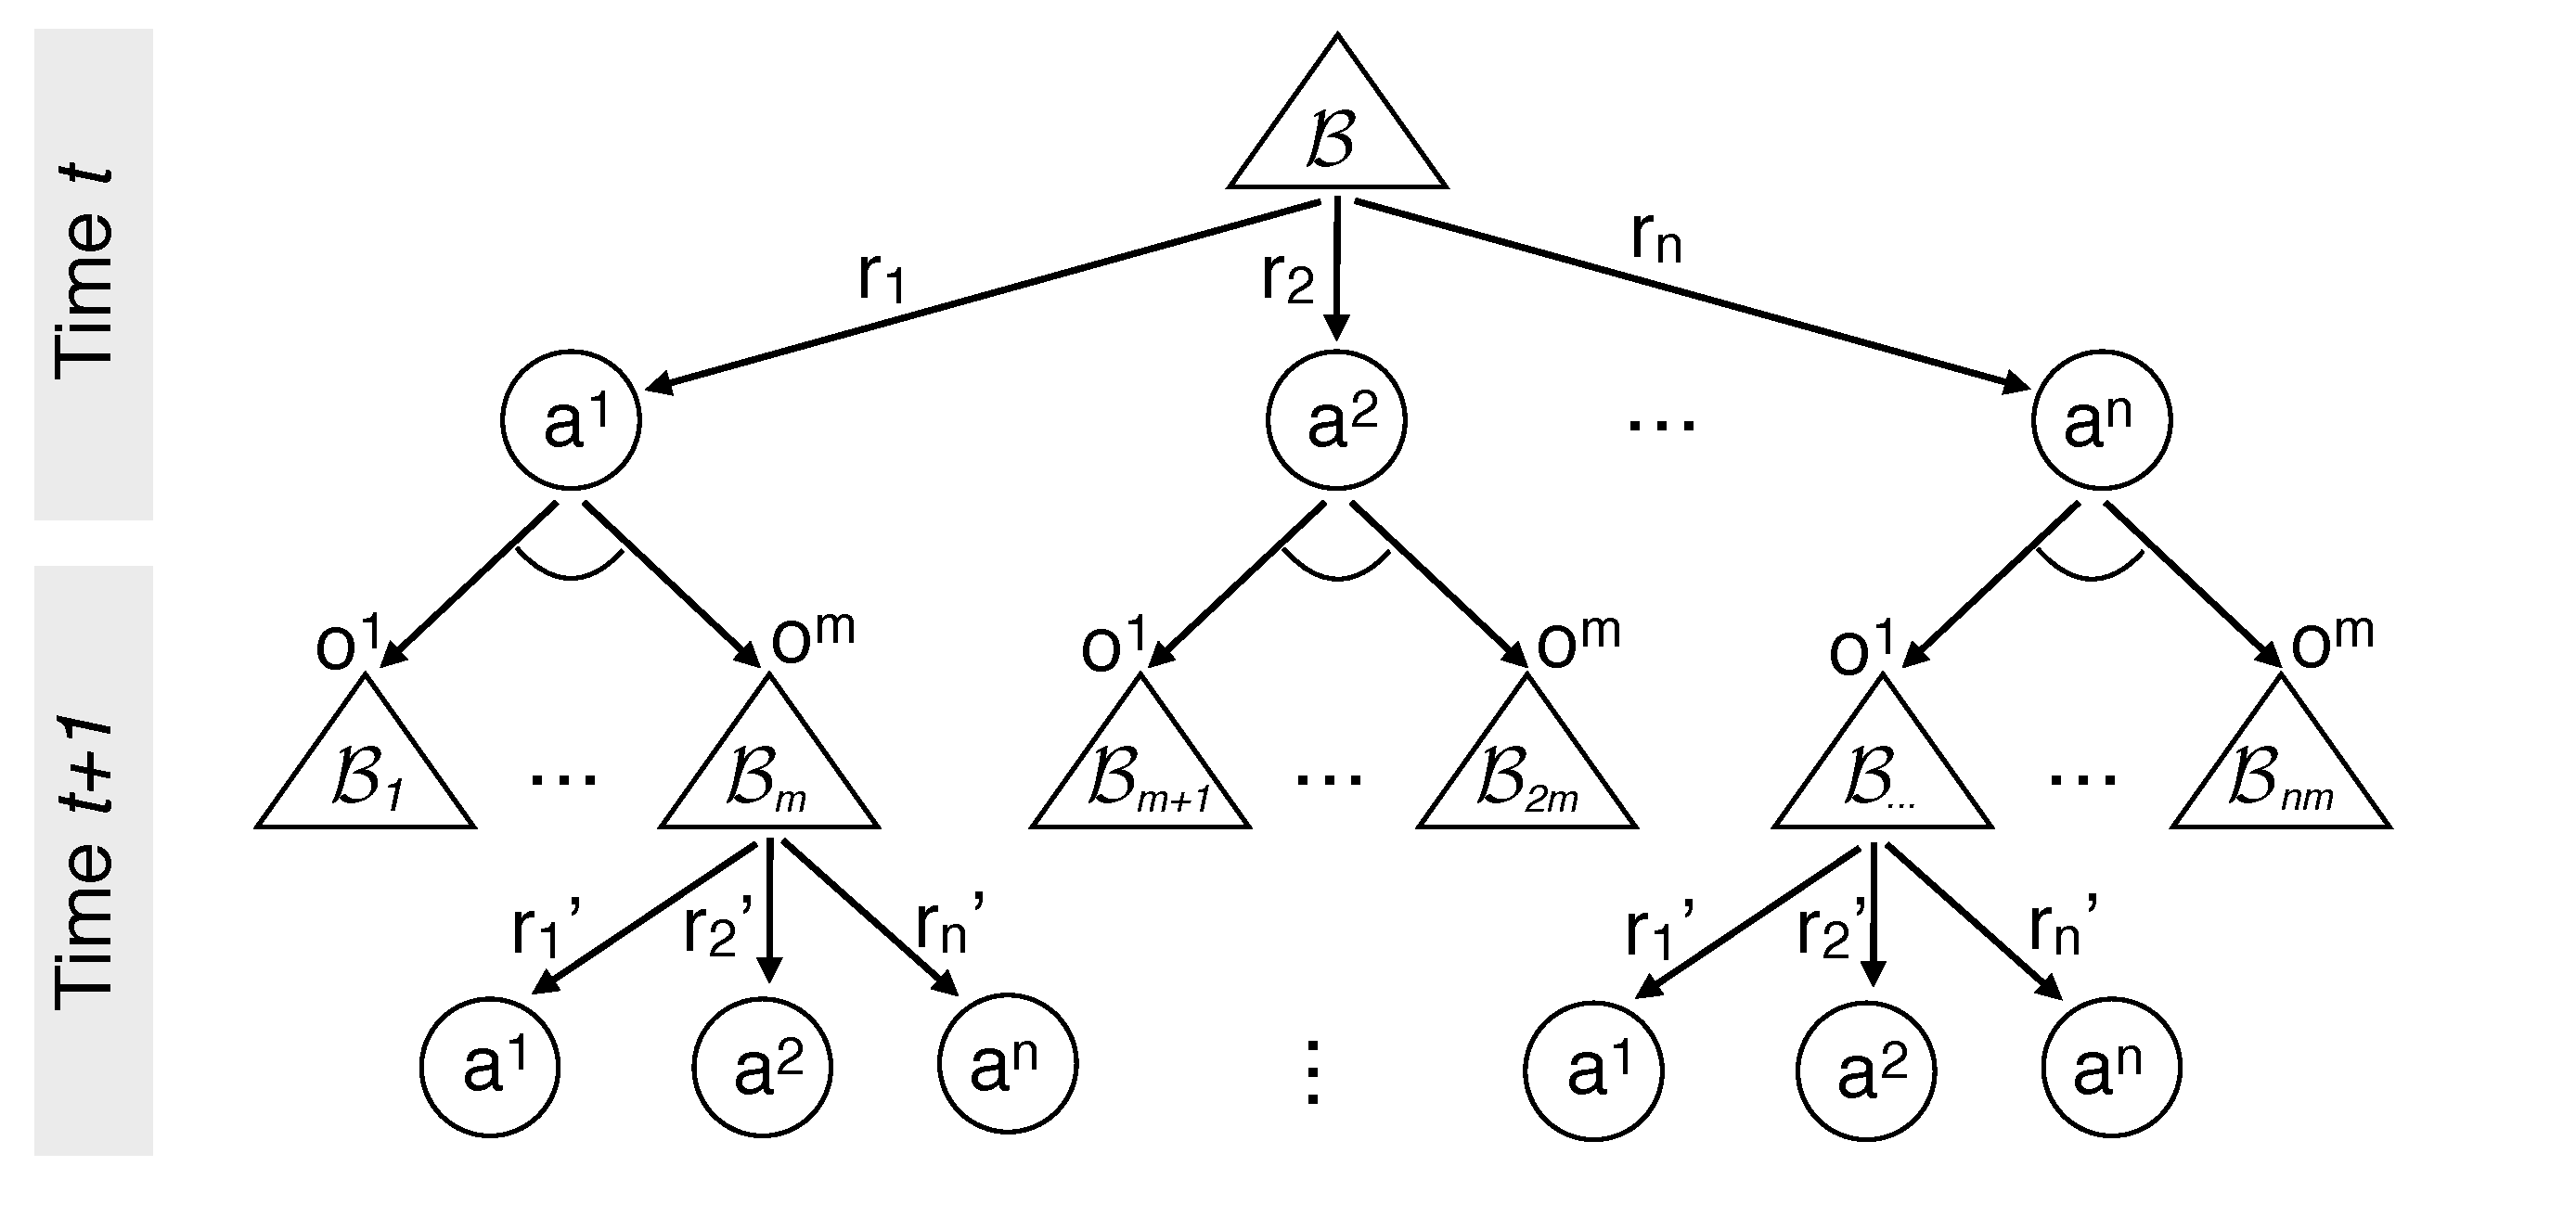
\includegraphics[scale=0.30]{imgs/andortree.pdf}
\caption{AND-OR search tree constructed through forward planning for a horizon of 2.}
\label{fig:andortree}
\end{figure}

Our implementation of Algorithms \ref{algo:planning} and \ref{algo:qval} operates in anytime mode\index{anytime algorithm} and expands the search tree by gradually adding new observations and actions in a breadth-first manner. At any point in time, the planning algorithm is thus able to deliver a solution. The quality of the solution will of course depend on the accuracy of the search tree, which itself depends on the number of sampled actions and observations -- more trajectories leading to a more accurate plan, but at a higher computational cost.  The anytime nature of the algorithm is important since the planner operates online.

As argued in \cite{onlineplanning-iwsds2012}, the reliance on utility rules to encode the reward model can help making the planning process more tractable.  In addition to assigning utilities to system actions, utility rules also implicitly define the set of action values that are relevant at a given time.\footnote{Recall that in Algorithm \ref{algo:instantiateUtilRule} from Section \ref{sec:ruleinstantiation}, the set of possible values of an action node is directly derived from the values listed in the utility nodes connected to it.} In other words, actions that are not deemed relevant in a particular state are automatically filtered out from the planning process.  Instead of searching through the whole space of possible actions, the planning algorithm is thus limited to a subset of actions that are locally relevant.\index{action selection!filtering of relevant actions}  One interesting aspect of this approach is that the filtering of relevant actions is done solely on the basis of the provided reward model and does not require the integration of additional constraints or ad-hoc mechanisms. This stands in contrast with most existing work in dialogue management, where constraints on possible actions are typically enforced through external filtering techniques defined on the basis of e.g.\ information-state update rules \citep{heeman2007}, finite-state automata \citep{williams2008}, or -- in our own previous work on this problem -- high-level constraints encoded in Markov Logic\index{Markov logic network} formulae \citep{srw-acl2010}. 

 
\subsubsection*{Learning cycle}
\index{parameter estimation}

The model-based learning cycle is detailed in Algorithm \ref{algo:rlearning_mb}. The learning agent incrementally updates its model parameters $\boldsymbol\theta$  by running a number of interactions, either with a real user or in simulation. Starting with an initial dialogue state, the interaction alternates between the reception of new observations (in the form of e.g.\ user inputs or contextual changes in the environment) and the execution of system actions following these observations.  The dialogue state is updated after each observation (line 5), using the procedure outlined in Section \ref{sec:processing-workflow}, with the action selection method replaced by Algorithm \ref{algo:planning}. The selected actions are then executed (line 7).   If the reward model is unknown, the reward resulting from the system actions can be integrated in the set of observations and used to update the reward parameters accordingly. 

\begin{algorithm}[ht]
\caption{: \textsc{Model-based-RL-learning} ($\mathcal{M}, \mathcal{B}_0, \boldsymbol\theta, N$)}
\begin{algorithmic}[1]\vspace{1mm}
\REQUIRE Rule-structured models $\mathcal{M}$ for the domain
\REQUIRE Initial dialogue state $\mathcal{B}_0$
\REQUIRE Model parameters $\boldsymbol\theta$ with prior distribution $P(\boldsymbol\theta)$
\REQUIRE Number $N$ of interactions to collect
\ENSURE Posterior distribution $P(\boldsymbol\theta)$ for the parameters  \vspace{1mm}
\FOR {$i = 0 \to N$}
\STATE Start new interaction with initial state $\mathcal{B} = \mathcal{B}_0 \cup \boldsymbol\theta $
\WHILE {interaction is active}
\STATE Get new observations $\mathbf{O}$
\STATE \textsc{UpdateState}($\mathcal{B}, \mathbf{O}$)
\IF {non-empty selected action $a$ in $\mathcal{B}$}
\STATE Execute action $a$ and get resulting reward $r$
\ENDIF
\ENDWHILE
\ENDFOR
\RETURN $P(\boldsymbol\theta)$
\end{algorithmic} 
\label{algo:rlearning_mb}
\end{algorithm}



\subsection{Model-free approach}
\label{sec:modelfree}
\index{rule parameters!model-free RL of}

In parallel to the model-based learning strategy described above, we also developed an alternative Bayesian model-free approach to the estimation of rule parameters.  In this approach, the core model that is to be estimated is the \textit{action--value model}\index{action--value model} which specifies the expected cumulative reward $Q$ of the system actions depending on the current state. 

In addition to this action--value model, the domain may also include transition and observation models. However, the transition and observation models are in model-free approaches only used for state update (if the dialogue state contains hidden state variables that are indirectly inferred from observations, such as the user intentions) and are not exploited in the action selection.  This stands in contrast with model-based approaches to reinforcement learning where transition and observation  models are directly employed to plan the next action.

\begin{wrapfigure}[14]{r}{60mm}
\vspace{-2mm}
\centering
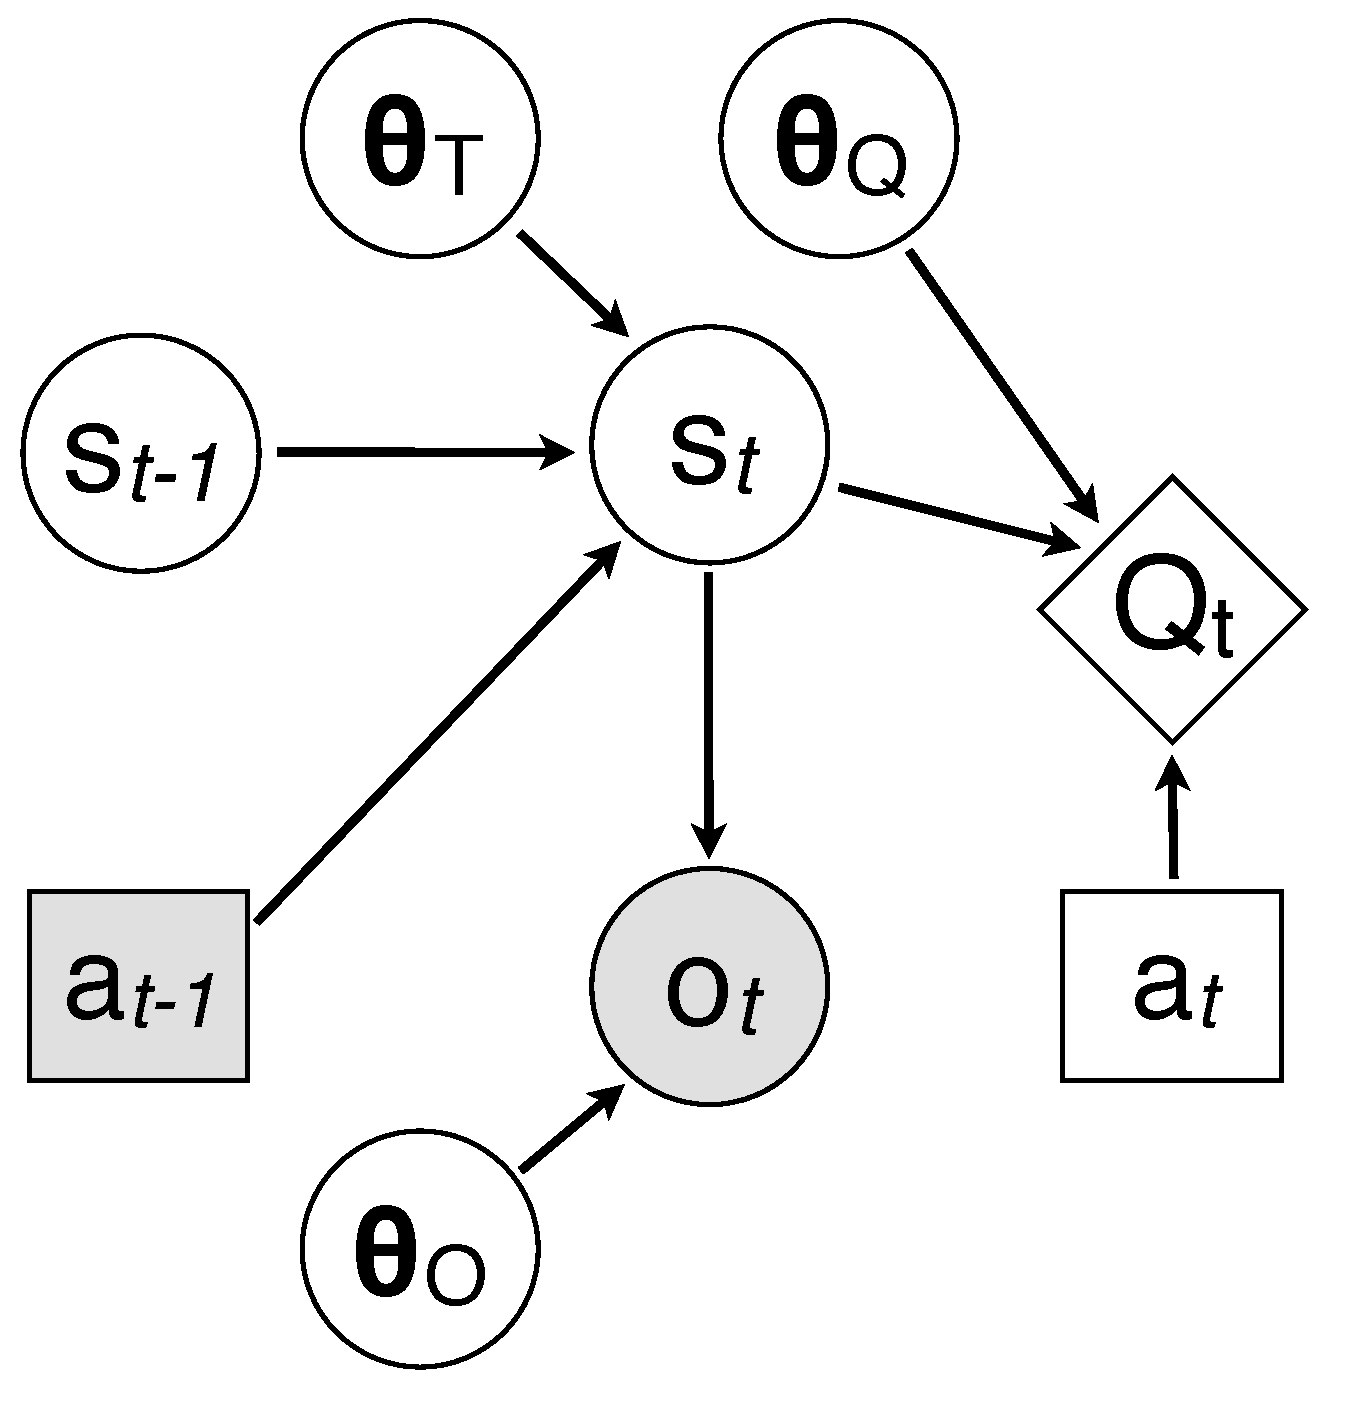
\includegraphics[scale=0.25]{imgs/modelfreediagram.pdf}
\vspace{-2mm}
\caption{Dynamic decision network for a model-free strategy.}
\label{fig:modelfreediagram}
\end{wrapfigure}

Figure \ref{fig:modelfreediagram} illustrates how these distributions combine to form a dynamic decision network\index{dynamic decision network}. As for the model-based approach, all domain models are specified with probabilistic rules\index{probabilistic rule} (which are again abstracted away from the simplified diagram in the figure). The transition and observation models are encoded by probability rules and the action--value model by utility rules. 

In the worst case, all models may include unknown parameters.  The transition model is thus defined as a probability distribution $P(s_t \, | \, s_{t\mbox{-}1}, a_{t\mbox{-}1} \,; \boldsymbol\theta_T)$, the observation model by a distribution $P(o_t \, | \, s_t\,; \boldsymbol\theta_O)$ and the $Q$ value model by a distribution $Q_t(s_t,a_t\,; \boldsymbol\theta_Q)$.  

\subsubsection*{Parameter estimation}
\index{parameter estimation}

The transition and observation models can be estimated in the same manner as in the model-based approach -- that is, by including the parameters in the dialogue state and refining their distributions as part of the state update process. 

The estimation of the action--value model is, however, slightly more intricate, since the $Q$ values are not directly accessible to the learning agent.  The only feedback perceived by the agent are indeed the immediate rewards resulting from its actions and the subsequent observations, not the expected cumulative rewards $Q$.  A solution to this estimation problem is to rely on Bellman's equation to incrementally improve the action--value estimates on the basis of the rewards resulting from the agent actions. Such methods are called temporal-difference methods and include many popular reinforcement learning algorithms such as SARSA and Q-learning\index{Q-learning} \citep{citeulike:112017}. Temporal-difference methods\index{temporal-difference methods} are also called ``boostrapping'' methods as they approximate new $Q$ value estimates based on previously learned estimates.

The particular model-free learning method applied in this work is based on the well-known SARSA algorithm.\index{SARSA}\footnote{SARSA stands for ``State-Action-Reward-State-Action'', as a reference to the algorithm's processing sequence.} The classical, MDP-based definition of SARSA proceeds as follows. Let $s_t$ be a dialogue state at time $t$, followed by a system action $a_t$. The execution of the system action $a_t$ results in a reward $r_{t+1}$ and a new dialogue state $s_{t+1}$ which is itself followed by a second system action $a_{t+1}$.  The SARSA update of the $Q$ value estimate for the first action $a_t$ is:
\begin{equation}
Q(s_t, a_t) \leftarrow Q(s_t,a_t) + \alpha \left[r_{t+1} + \gamma \ Q(s_{t+1}, a_{t+1}) - Q(s_t, a_t) \right] 
\end{equation}
where $\alpha$ represents the learning rate of the algorithm. The estimate $Q(s_t, a_t)$ is thus modified in direction of the value $ \left[r_{t+1} + \gamma \ Q(s_{t+1}, a_{t+1} \right]$, with a learning step expressed by $\alpha$. 

%As shown by e.g.\ \cite{Dearden:1998}, temporal-difference methods are easily amenable to a Bayesian treatment. 

The approach developed in this thesis rests on a simple Bayesian extension of SARSA.  The posterior distribution over the parameters is here computed on the basis of the evidence provided by the reward $r_{t+1}$ and next system action $a_{t+1}$.  Given a sequence of state--action-rewards $\langle \mathcal{B}_t, a_t, r_{t+1}, \mathcal{B}_{t+1}, a_{t+1} \rangle$, we define the likelihood distribution $P(r_{t+1}, a_{t+1} \,; \boldsymbol\theta)$ as:
\begin{equation}
P(r_{t+1}, a_{t+1} \,; \boldsymbol\theta) = \phi \left(\frac{r_{t+1} + \gamma \ Q_{\mathcal{B}_{t+1}} \left(a_{t+1} \,; \boldsymbol\theta\right) - Q_{\mathcal{B}_t}\left(a_t \,; \boldsymbol\theta\right)}{\sigma} \right) \label{eq:modelfreelikelihood}
\end{equation}
where $\phi(\cdot)$ is the density function for the standard normal distribution $\mathcal{N}(0, 1)$.\index{normal distribution} The standard normal distribution has its peak around the value 0 and decreases exponentially with the distance to this mean. The likelihood distribution will therefore yield a high probability when the initial estimate 
$Q_{\mathcal{B}_t}(a_t \,; \boldsymbol\theta)$ available at time $t$ is close to the updated estimate $\left[r_{t+1} + \gamma \ Q_{\mathcal{B}_{t+1}} (a_{t+1} \,; \boldsymbol\theta) \right]$ at time $t+1$, and a low probability otherwise. The variance $\sigma$ encodes the spread of the bell curve and controls as a consequence the learning rate.

Based on the likelihood distribution defined in Equation \eqref{eq:modelfreelikelihood}, the posterior distribution on the parameters is finally rewritten as: \index{posterior parameter distribution}
\begin{equation}
P(\boldsymbol\theta \, | \, r_{t+1}, a_{t+1}) = \eta \ P(r_{t+1}, a_{t+1} \,; \boldsymbol\theta)  \ P(\boldsymbol\theta)  \label{eq:posteriormodelfree}
\end{equation}


\subsubsection*{Action selection}
\index{action selection}
\index{$\epsilon$-greedy strategy}

The above section described how the parameter distributions are updated on the basis of the received rewards and executed actions, but did not explain how the system actions were selected at runtime.  A simple strategy is to select the action yielding the maximum $Q$ value for the current state.  This pure greedy strategy can, however, result in poor control policies whenever the agent gets stuck in a suboptimal behaviour.  Greedy strategies can be improved by allowing the agent to explore other actions once in a while. The relative frequency of these exploration actions compared to the  ``greedy'' actions is expressed by the probability $\epsilon$, which is usually small. This method is called an $\epsilon$-greedy strategy and is illustrated in Algorithm \ref{algo:egreedy}.

\begin{algorithm}[h!]
\caption{: \textsc{$\epsilon$-Greedy-Policy} ($\mathcal{B}, \mathbf{e}$)}
\begin{algorithmic}[1] \vspace{1mm}
\REQUIRE Dialogue state $\mathcal{B}$ as a decision network
\REQUIRE Evidence $\mathbf{e}$
\ENSURE Selected action $\mathbf{a}^*$
\STATE Select value $\mathbf{a}^* = \begin{cases} \argmax_{\mathbf{a}} Q(\mathbf{a}, \mathbf{e}) & \text{with probability } (1- \epsilon) \\ \text{another action} & \text{with probability } \epsilon \end{cases}$
\STATE Remove utility nodes from the state $\mathcal{B}$
\RETURN $\mathbf{a}^*$
\end{algorithmic}
\label{algo:egreedy}
\end{algorithm}

\subsubsection*{Learning cycle}
\index{parameter estimation}

The model-free learning cycle is mostly similar to the one defined in the model-based setting.  As shown in Algorithm \ref{algo:rllearning_modelfree}, the agent estimates the values of its rule parameters by collecting a number of interactions.  Each interaction starts from the initial dialogue state $\mathcal{B}_0$ and unfolds as a sequence of observations and actions.  The dialogue state contains both traditional state variables and parameter variables.  After perceiving new observations, the dialogue state is correspondingly updated -- including transition and observation parameters if present in the domain (line 5).  The update process comprises the selection of new system actions, according to the $\epsilon$-greedy selection procedure shown in Algorithm \ref{algo:egreedy}. When a new action is selected, the posterior distributions over parameters are correspondingly updated through temporal-difference learning (line 7). The action is then executed and the resulting reward is retrieved (line 8).  The process is repeated for each interaction. 


\begin{algorithm}[ht]
\caption{\textsc{Model-free-RL-learning} ($\mathcal{M}, \mathcal{B}_0, \boldsymbol\theta, N$)}
\begin{algorithmic}[1]\vspace{1mm}
\REQUIRE Rule-structured models $\mathcal{M}$ for the domain
\REQUIRE Initial dialogue state $\mathcal{B}_0$
\REQUIRE Model parameters $\boldsymbol\theta$ with prior distribution $P(\boldsymbol\theta)$
\REQUIRE Number $N$ of interactions to collect
\ENSURE Posterior distribution $P(\boldsymbol\theta)$ for the parameters  \vspace{1mm}
\FOR {$i = 0 \to N$}
\STATE Start new interaction with initial state $\mathcal{B} = \mathcal{B}_0 \cup \boldsymbol\theta $
\WHILE {interaction is active}
\STATE Get new observations $\mathbf{O}$
\STATE \textsc{UpdateState}($\mathcal{B}, \mathbf{O}$)
\IF {non-empty selected action $a$ in $\mathcal{B}$}
\STATE Update posterior $P(\boldsymbol\theta \, | \, r, a)$ based on Equation \eqref{eq:posteriormodelfree}
\STATE Execute action $a$ and get resulting reward $r$
\ENDIF
\ENDWHILE
\ENDFOR
\RETURN $P(\boldsymbol\theta)$
\end{algorithmic} 
\label{algo:rllearning_modelfree}
\end{algorithm}


\section{Experiments}
\label{sec:rllearning-experiments}

We performed an empirical evaluation of the two approaches based on a user simulator\index{user simulator} for a human--robot interaction\index{human--robot interaction} domain. The evaluation is divided in two parts: 
\begin{enumerate}
\item The goal of the first experiment was to determine whether the use of probabilistic rules could be shown to improve the performance of a reinforcement learning agent.  More specifically, the experiment compared two alternative formalisations of a transition model for a human--robot interaction scenario: one encoded with traditional categorical distributions, and one encoded with probability rules.  

\item The goal of the second experiment focused on the comparison between model-based and model-free approaches in Bayesian reinforcement learning. The evaluation compared a model-based learner with an unknown transition model (such as the one used in the first experiment) to a model-free learner with an unknown action--value model.  Both strategies relied on probabilistic rules to capture their respective models and were evaluated on the basis of their average rewards when interacting with the user simulator. 
\end{enumerate}

We first describe in this section the dialogue domain and user simulator used in both experiments, and then detail the evaluation setups and empirical results for each experiment. 

\subsection{Dialogue domain}
\label{sec:exp2_dd}
\index{dialogue domain}
As in the previous chapter, the dialogue domain chosen for the experiments is a human--robot interaction scenario with a Nao robot.\index{Nao robot}  The interactions collected for the experiments involved the Nao robot conversing with a human user in a shared visual scene including a few graspable visual objects, as illustrated in Figure \ref{fig:naochap6}.  The users were instructed to command the robot to carry the objects from one place to another. The users were free to decide which object(s) to pick up, where to place them on the floor, and what kinds of navigation commands to provide to perform the task.  In addition to following the human instructions, the robot could also answer factual questions from the user regarding its own knowledge of the environment such as \utt{do you see a blue cylinder?} or \utt{what do you see?}. 

Each (physical or information-gathering) sub-task is represented as a distinct user intention. As the human users could only instruct the robot to perform one sub-task at a time, the user intention is represented by a single variable denoting the current sub-task that the user wish to see fulfilled.  The user intentions for the domain are listed in Table \ref{table:userintents_exp2}. 

\begin{figure}[ht]
$\phantom{a}$ \\[2mm]
\centering
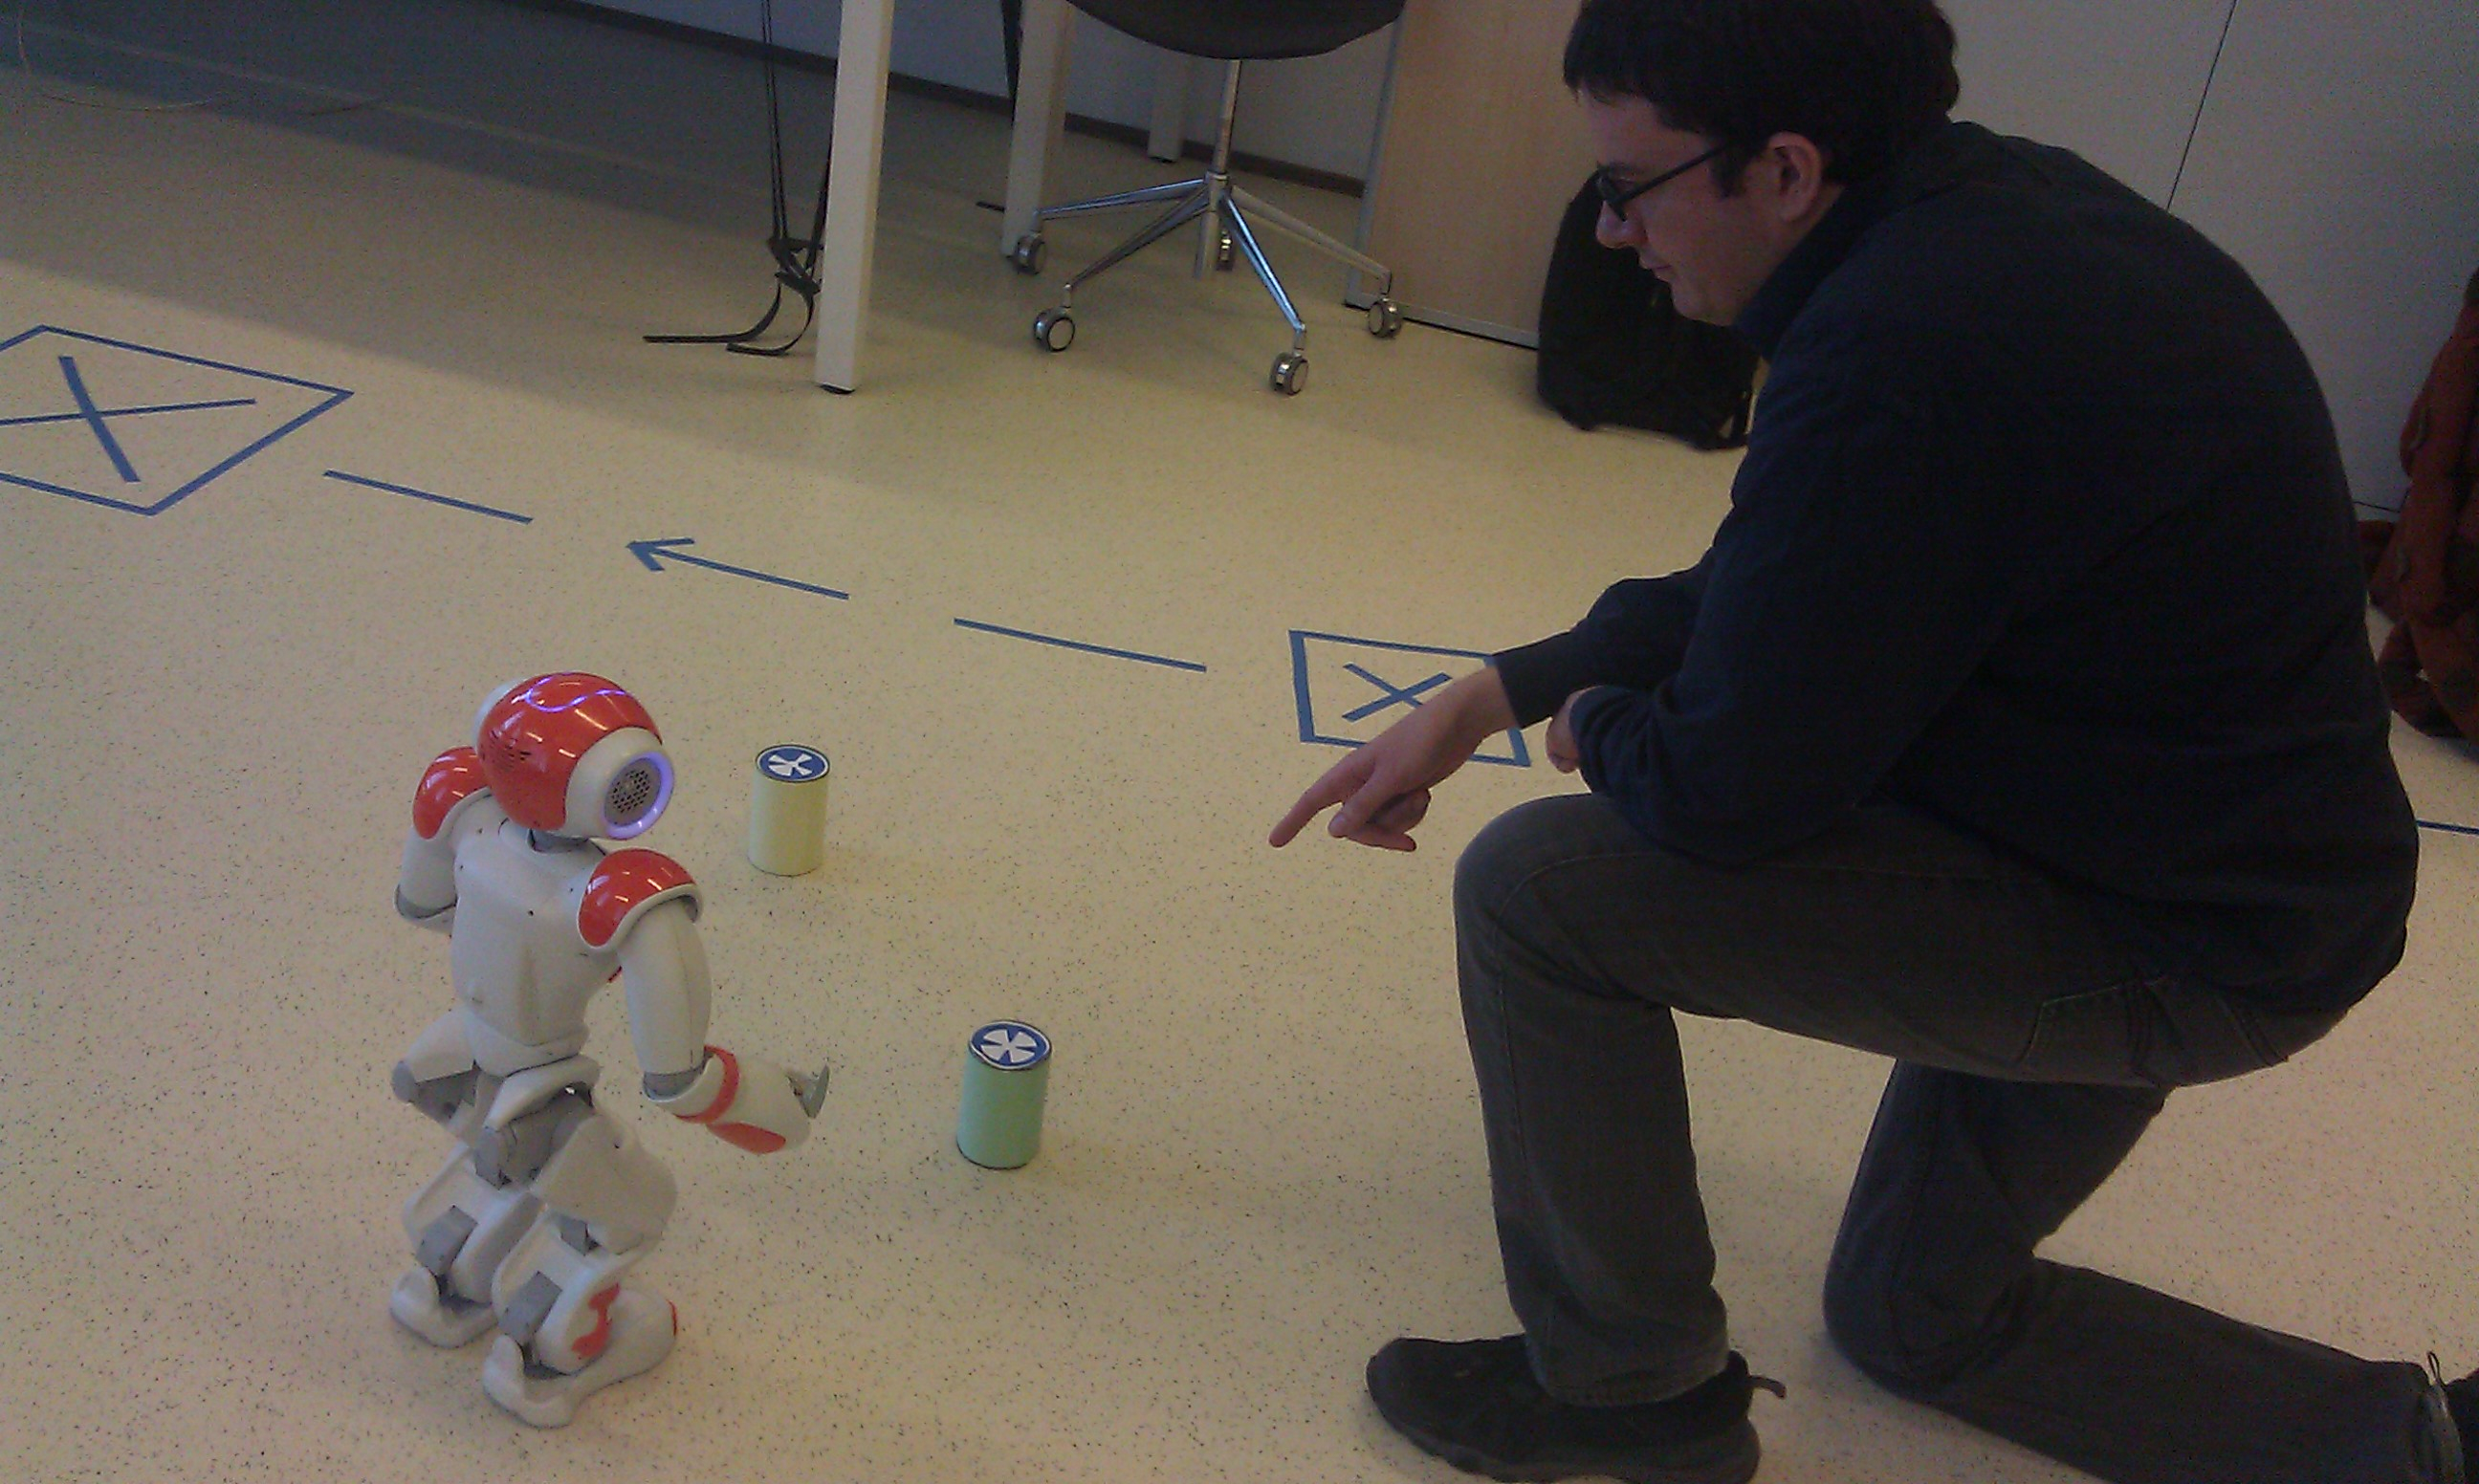
\includegraphics[scale=0.12]{imgs/jonathon2.jpg}
\caption{Human user interacting with the Nao robot in a shared visual scene with two objects.}
\label{fig:naochap6}
\end{figure}

The objects in the scene consisted of coloured metallic cylinders with a special marking on their top to facilitate the robot's visual servoing during grasping tasks.  As the version of the Nao robot employed in the experiments did not include actuated fingers, the grasping operation employed permanent magnets attached to the robot hands to grasp and carry the cylinders.

In addition to following the user commands related to spatial navigation and object manipulation, the robot could also perform grounding-related actions such clarification requests and acknowledgements. In total, the domain included 9 user dialogue templates\index{dialogue acts}.  The robot has a repertoire of 8 possible action templates that can be executed.  For a dialogue domain with two objects, the user actions $a_u$ and system actions $a_m$ will thus expand into respectively 15 and 37 actions.  Tables \ref{table:userdas_exp2} and \ref{table:systemdas_exp2} list the possible user and system actions.

\renewcommand{\arraystretch}{1.3}

\begin{table}[p]
\begin{footnotesize}
\begin{tabular}{p{60mm}} 
$\cdot$ $\mathrm{Move}(x) $ \\ $ \ \ \ \ \ \text{ where } x=\{\mathrm{Left,Right,Forward,}$ \\ $\ \ \ \ \ \ \ \ \ \ \ \ \ \ \ \ \ \ \ \ \ \ \ \ \ \mathrm{Backward}\} $ \\ 
$\cdot$ $\mathrm{PickUp}(x) $ \\ $\ \ \ \ \  \text{ where } x \text{ is an object identifier}$ 
\end{tabular}
\hspace{2cm}
\begin{tabular}{p{60mm}} 
$\cdot$ $\mathrm{Release}(x) $ \\ $\ \ \ \ \  \text{ where } x \text{ is an object identifier}$ \\
$\cdot$ $\mathrm{WhatDoYouSee}$ \\
$\cdot$ $\mathrm{DoYouSee}(x) $ \\ $\ \ \ \ \  \text{ where } x \text{ is an object identifier}$ 
\end{tabular}
\end{footnotesize}
 \caption{List of user intentions $i_u$.} 
\label{table:userintents_exp2}
\end{table}


\begin{table}[p]
\begin{footnotesize}
\begin{tabular}{p{60mm}} 
$\cdot$ $\mathrm{Ask(Move(x))} $ \\ $ \ \ \ \ \ \text{ where } x=\{\mathrm{Left,Right,Forward,}$ \\ $\ \ \ \ \ \ \ \ \ \ \ \ \ \ \ \ \ \ \ \ \ \ \ \ \ \mathrm{Backward}\} $ \\ 
$\cdot$ $\mathrm{Ask(PickUp(x))} $ \\ $\ \ \ \ \  \text{ where } x \text{ is an object identifier}$ \\
$\cdot$ $\mathrm{Ask(Release(x))} $ \\ $\ \ \ \ \  \text{ where } x \text{ is an object identifier}$ 
\end{tabular}
\hspace{2cm}
\begin{tabular}{p{60mm}} 
$\cdot$ $\mathrm{RepeatLastMove}$ \\
$\cdot$ $\mathrm{Ask(WhatDoYouSee)}$ \\
$\cdot$ $\mathrm{Ask(DoYouSee(x))} $ \\ $\ \ \ \ \  \text{ where } x \text{ is an object identifier}$ \\
$\cdot$ $\mathrm{Confirm}$ \\
$\cdot$ $\mathrm{Disconfirm}$ \\
$\cdot$ $\mathrm{Other}$ 
\end{tabular}
\end{footnotesize}
 \caption{List of user actions $a_u$.} 
\label{table:userdas_exp2}
\end{table}

\begin{table}[p]
\begin{footnotesize}
\begin{tabular}{p{60mm}} 
$\cdot$ $\mathrm{Do}(x) $ \\ $ \ \ \ \text{ where } x=\{\mathrm{Move}(y),\mathrm{PickUp}(z),$  \\ $\ \ \ \ \ \ \ \ \ \ \ \ \ \ \ \ \ \ \ \ \ \ \ \mathrm{Release}(z)\} $ \\ $ \ \ \ \ \ \ \text{ and } y = \{\mathrm{Left,Right,Forward,}$ \\ $ \ \ \ \ \ \ \ \ \ \ \ \ \ \ \ \ \ \ \ \ \ \ \ \mathrm{Backward}\} $ \\ $ \ \ \ \ \ \  \text{ and } z = \ \text{an object identifier}$ \\
$\cdot$ $\mathrm{Excuse}(x) $ \\ $ \ \ \  \text{ where } x = \{\mathrm{DoNotSeeObject}$ \\ $\ \ \ \ \ \ \ \ \ \ \ \ \ \ \ \ \ \ \ \ \ \ \ \mathrm{DoNotCarryObject,}$ \\ $\ \ \ \ \ \ \ \ \ \ \ \ \ \ \ \ \ \ \ \ \ \ \ \mathrm{AlreadyCarryObject}\}$ \\
$\cdot$ $\mathrm{Describe}(x) $ \\ $ \ \ \  \text{ where } x = \ \text{a (possibly empty) list}$ \\ $ \ \ \ \ \ \ \ \ \ \ \ \ \ \ \ \ \ \ \ \ \ \ \  \text{of object identifiers}$ \\
$\cdot$ $\mathrm{ConfirmDetection}$ \\
$\cdot$ $\mathrm{DisconfirmDetection}$ 
\end{tabular}
\hspace{2cm}
\begin{tabular}{p{60mm}} 
$\cdot$ $\mathrm{Ground}(x) $ \\ $ \ \ \ \text{ where } x=\{\mathrm{Move}(y),\mathrm{PickUp}(z),$  \\ $\ \ \ \ \ \ \ \ \ \ \ \ \ \ \ \ \ \ \ \ \ \ \ \mathrm{Release}(z)\} $ \\ $\ \ \ \ \ \  \text{ and } y = \{\mathrm{Left,Right,Forward,}$ \\ $\ \ \ \ \ \ \ \ \ \ \ \ \ \ \ \ \ \ \ \ \ \ \  \mathrm{Backward}\} $ \\ $\ \  \ \ \ \ \text{ and } z = \ \text{an object identifier}$ \\
$\cdot$ $\mathrm{AskClarify}$ \\
$\cdot$ $\mathrm{AskConfirm}(x) $ \\ $\ \ \ \text{ where } x=\{\mathrm{Move}(y),\mathrm{PickUp}(z),$  \\ $\ \ \ \ \ \ \ \ \ \ \ \ \ \ \ \ \ \ \ \ \ \ \ \mathrm{Release}(z), \mathrm{DoYouSee}(z),$ \\ $ \ \ \ \ \ \ \ \ \ \ \ \ \ \ \ \ \ \ \ \ \ \ \ \mathrm{WhatDoYouSee} \} $ \\ $\ \ \ \ \ \  \text{ and } y = \{\mathrm{Left,Right,Forward,}$ \\ $\ \ \ \ \ \ \ \ \ \ \ \ \ \ \ \ \ \ \ \ \ \ \  \mathrm{Backward}\} $ \\ $\ \ \ \ \ \  \text{ and } z = \ \text{an object identifier}$ \
\end{tabular}
\end{footnotesize}
 \caption{List of system actions $a_m$.} 
\label{table:systemdas_exp2}
\end{table}

Transcript 3 provides a detailed example of recorded interaction between a human user and the (wizard-controlled) robot.

\begin{Transcript}[p]
\begin{dialogue} \vspace{3mm}
\speak{Robot} Hello human\vspace{2mm}
\speak{Human} Hi, hello Lenny! \vspace{1mm} \\ 
\direct{\refer{Robot} stands up} \vspace{2mm}
\speak{Human} Would you please move forward\vspace{2mm}
\speak{Robot} OK, moving forward  \vspace{1mm} \\
\direct{\refer{Robot} steps forward} \vspace{2mm}
\speak{Human} Would you please move a bit more forward\vspace{2mm}
\speak{Robot} Should I move backward \vspace{2mm}
\speak{Human} No, a bit more forward\vspace{2mm}
\speak{Robot} OK, forward then \vspace{1mm} \\ 
\direct{\refer{Robot} steps forward} \vspace{2mm}
\speak{Human} Do you see any object?\vspace{2mm}
\speak{Robot} Sorry I do not understand\vspace{2mm}
\speak{Human} Do you see any object?\vspace{2mm}
\speak{Robot} I see a blue cylinder\vspace{2mm}
\speak{Human} Can you pick it up please?\vspace{2mm}
\speak{Robot} Should I pick up the object?\vspace{2mm}
\speak{Human} Yes please\vspace{2mm}
\speak{Robot} OK, thanks  \vspace{1mm} \\
\direct{\refer{Robot} moves in direction of the blue cylinder} \\
\direct{\refer{Robot} picks up the object} \vspace{2mm}
\speak{Robot} Done\vspace{2mm}
\speak{Human} Now turn right \vspace{1mm} \\ 
\direct{\refer{Robot} turns right while holding the object} \vspace{2mm}
\speak{Human} Move forward \vspace{1mm} \\ 
\direct{\refer{Robot} moves forward while holding the object} \vspace{2mm}
\speak{Human} And then move two steps backward\vspace{2mm}
\speak{Robot} OK, moving forward\vspace{1mm} \\
\direct{\refer{Robot} starts movement} \vspace{2mm}
\speak{Human} No please move backward \vspace{1mm} \\ 
\direct{\refer{Robot} stops} \vspace{2mm}
\end{dialogue}
\vspace{-4mm} \hspace{1cm}\direct{...} \vspace{3mm}
\caption{User interaction with wizard-controlled robot}
\end{Transcript}

The reward model\index{reward model} was defined by hand, using standard schemes: The execution of correct actions or the correct answer to user questions leads to large positive values (+6 in this particular case) while the execution of wrong or irrelevant actions leads to large negative values (-6) and the use of clarification or confirmation requests to small negative values (from -0.5 to -1.5, depending on the type of request). Table \ref{table:rewards} presents the reward model defined for the domain. 


\begin{table}[ht]
\begin{center}
\begin{footnotesize}
\begin{tabular}{p{130mm}c} 
\centering \textbf{Action} & \textbf{Reward} \\
Execution of correct physical action $a_m\!=\!\mathrm{Do}(i_u)$ & +6 \\
Execution of wrong physical action $a_m\!=\!\mathrm{Do}(x)$ with $x\!\neq\!i_u$ & -6  \\
Declare $a_m\!=\!\mathrm{Excuse(DoNotSeeObject})$ when $i_u\!=\!\mathrm{PickUp}(x)$ and $x$ is not perceived & +6 \\
Declare $a_m\!=\!\mathrm{Excuse(DoNotCarryObject})$ when $i_u\!=\!\mathrm{Release}(x)$ and $x$ is not carried & +6 \\
Declare $a_m\!=\!\mathrm{Excuse(AlreadyCarryObject})$ when $i_u\!=\!\mathrm{PickUp}(x)$ and $x$ is carried & +6 \\
Declare $a_m\!=\!\mathrm{Excuse(*})$ in other circumstances & -6 \\
Correct answer $a_m\!=\!\mathrm{Describe}(x)$ when $i_u\!=\!\mathrm{WhatDoYouSee}$ and $x$ are the perceived objects & +6 \\
Wrong answer $a_m\!=\!\mathrm{Describe}(*)$ when $i_u\!\neq\!\mathrm{WhatDoYouSee}$ & -6 \\
Correct answer $a_m\!=\!\mathrm{ConfirmDetection}$ when $i_u\!=\!\mathrm{DoYouSee(x)}$ and $x$ is perceived & +6 \\
Wrong answer $a_m\!=\!\mathrm{ConfirmDetection}$ when $i_u\!\neq\!\mathrm{DoYouSee(x)}$ or $x$ is not perceived & -6 \\
Correct answer $a_m\!=\!\mathrm{DisconfirmDetection}$ when $i_u\!=\!\mathrm{DoYouSee(x)}$ and $x$ is not perceived & +6 \\
Wrong answer $a_m\!=\!\mathrm{DisconfirmDetection}$ when $i_u\!\neq\!\mathrm{DoYouSee(x)}$ or $x$ is perceived & -6 \\
Grounding of correct intention $a_m\!=\!\mathrm{Ground}(i_u)$ & +2 \\
Grounding of wrong intention  $a_m\!=\!\mathrm{Ground}(x)$ with $x\!\neq\!i_u$ & -6  \\ 
Request to confirm correct intention $a_m\!=\!\mathrm{AskConfirm}(i_u)$ & -0.5 \\
Request to confirm wrong intention  $a_m\!=\!\mathrm{AskConfirm}(x)$ with $x\!\neq\!i_u$ & -1.5  \\ 
Request to clarify $a_m\!=\!\mathrm{AskClarify}$ & -1 \\
Ignore user act $a_m\!=\!\mathrm{None}$ when $a_u\!\neq\!\mathrm{None}$ & -1.5 
\end{tabular}
\end{footnotesize}
\end{center}  
\caption{Reward model for the domain.} 
\label{table:rewards}
\end{table}


\subsection{Simulator}
\index{user simulator}

\subsubsection*{Methodology}

In order to draw meaningful and reliable comparisons between reinforcement learning approaches, the user behaviours must be made fully consistent across interactions.  This consistency must be enforced on both the conversational choices of the user and the average amount of noise and comprehension errors that characterise them. Needless to say, this criteria is hard to satisfy when working with human participants. The comparative evaluation of learning approaches was thus conducted with the help of a simulator. However, it should be emphasised that the reliance on user simulators to conduct the comparative evaluation of our learning approaches does not in any way imply that simulators are a necessary component of the learning approach presented in this thesis.\footnote{In fact, probabilistic rules are expected to be well suited for optimisation from live interactions, as they require drastically less training data than traditional approaches (as evidenced by the empirical results in this section).}

The purpose of the simulator is to emulate the typical dialogue behaviour of a human user, and generate relevant user responses to the system actions.  In addition, the simulator also maintains a virtual representation of the environment during the interaction (represented in our case by the physical objects) and update this representation as a function of the system actions.


\subsubsection*{Wizard-of-Oz study}
\index{Wizard-of-Oz interaction}
\index{Wizard-of-Oz interaction!data collection}

In order to build a user simulator that matches as closely as possible the behaviour of actual human subjects, we started by recording a set of Wizard-of-Oz interactions in the human--robot dialogue domain chosen for the experiments. 

The technical setup employed for the Wizard-of-Oz data collection was mostly similar to the one described in the previous chapter, with one notable difference:  While the Wizard-of-Oz interactions described in Section \ref{sec:wozlearning-experiments-woz} served to determine the most appropriate \textit{system} actions depending on the situation, the goal of the Wizard-of-Oz interactions is here to collect empirical data about the most likely \textit{user} actions in their context.  As the wizard behaviour was not the focus of the study, the wizard had a direct access to the user utterances, without relying on the speech recogniser as an intermediary. The wizard controlled the verbal and physical actions via a remote screen coupled to the robotic platform. Various types of errors and misunderstandings were artificially introduced by the wizard in the course of the interaction in order to also gather data about the user responses to such comprehension errors. 

A total of eight interactions were recorded, each with a different speaker (5 males and 3 females), totalling about 50 minutes divided in 486 turns.  The interactions were performed in English. The users were again recruited amongst the local group of students and employees in the Department of Informatics at the University of Oslo and were (with one exception) non-native English speakers. The author of the present thesis served as the wizard. 

After the recording, the dialogues were segmented and annotated by hand. The first layer of annotation encodes the user dialogue acts $a_u$ and system actions $a_m$ listed in Table \ref{table:userdas_exp2} and \ref{table:systemdas_exp2}. The user intentions $i_u$ underlying the user commands are annotated on top of this sequence of turns.\footnote{Although the user intentions are in principle hidden ``mentalistic'' entities, they can in our domain be easily determined by a human annotator from the dialogue transcript.} The annotation also includes two contextual variables respectively expressing the lists of objects perceived and carried by the robot at a given time. Transcript 4 provides a concrete example of annotation for the first part of the interaction in Transcript 3. 

\begin{Transcript}[p]
\begin{dialogue} \vspace{5mm}
\speak{Human} Would you please move forward \\[1mm]
\begin{footnotesize}\textbf{Annotation}: $a_u\!=\!\mathrm{Ask(Move(Forward))}$\\ $\phantom{1}$\hspace{16mm} $i_u\!=\!\mathrm{Move(Forward)}, \mathit{carried}\!=\![],\mathit{perceived}\!=\![]$\end{footnotesize} \vspace{3mm}
\speak{Robot} OK, moving forward \\[1mm]
\begin{footnotesize}\textbf{Annotation}: $a_m\!=\!\mathrm{Ground(Move(Forward)) }  \ + \ \mathrm{ Do(Move(Forward))}$ \end{footnotesize}\vspace{3mm}
\speak{Human} Would you please move a bit more forward \\[1mm]
\begin{footnotesize}\textbf{Annotation}: $a_u\!=\!\mathrm{Ask(Move(Forward))}$\\$\phantom{1}$\hspace{16mm} $i_u\!=\!\mathrm{Move(Forward)}, \mathit{carried}\!=\![],\mathit{perceived}\!=\![\mathit{object}_1]$\end{footnotesize}\vspace{3mm}
\speak{Robot} Should I move backward \\[1mm]
\begin{footnotesize}\textbf{Annotation}: $a_m\!=\!\mathrm{AskConfirm(Move(Backward))}$\end{footnotesize} \vspace{3mm}
\speak{Human} No, a bit more forward \\[1mm]
\begin{footnotesize}\textbf{Annotation}: $a_u\!=\!\mathrm{Disconfirm } \ + \ \mathrm{ Ask(Move(Forward))}, $ \\$\phantom{1}$\hspace{16mm} $i_u\!=\!\mathrm{Move(Forward)}, \mathit{carried}\!=\![], \mathit{perceived}\!=\![\mathit{object}_1]$\end{footnotesize}\vspace{3mm}
\speak{Robot} OK, forward then \\[1mm] 
\begin{footnotesize}\textbf{Annotation}: $a_m\!=\!\mathrm{Ground(Move(Forward)) }  \ + \ \mathrm{ Do(Move(Forward))}$ \end{footnotesize} \vspace{3mm}
\speak{Human} Do you see any object? \\[1mm] 
\begin{footnotesize}\textbf{Annotation}: $a_u\!=\!\mathrm{Ask(WhatDoYouSee)},$\\ $\phantom{1}$ \hspace{16mm}$ i_u\!=\!\mathrm{WhatDoYouSee},\mathit{carried}\!=\![],\mathit{perceived}\!=\![\mathit{object}_1]$ \end{footnotesize} \vspace{3mm}
\speak{Robot} Sorry I do not understand \\[1mm]
\begin{footnotesize}\textbf{Annotation}: $a_m\!=\!\mathrm{AskClarify}$ \end{footnotesize}\vspace{3mm}
\speak{Human} Do you see any object? \\[1mm]
\begin{footnotesize}\textbf{Annotation}: $a_u\!=\!\mathrm{Ask(WhatDoYouSee)}, $ \\ $\phantom{1}$ \hspace{16mm}$i_u\!=\! \mathrm{WhatDoYouSee}, \mathit{carried}\!=\![],\mathit{perceived}\!=\![\mathit{object}_1]$\end{footnotesize} \vspace{3mm}
\speak{Robot} I see a blue cylinder \\[1mm]
\begin{footnotesize}\textbf{Annotation}: $a_m\!=\!\mathrm{Describe}([\mathit{object}_1])$ \end{footnotesize} \vspace{1mm}
\end{dialogue}
\caption{Annotated dialogue excerpt}
\end{Transcript}


\subsubsection*{User and context modelling}
\index{user modelling}
\index{context modelling}

After collecting and annotating the Wizard-of-Oz interactions, the next step in the development of the simulator is to design the transition model that determines how the user and the environment are to respond to the system actions. This statistical model is used at runtime to sample possible responses and feed them back to the dialogue system. 

The transition model\index{transition model} for our human--robot interaction dialogue domain is factored into four components:
\begin{enumerate}
\item a user goal model\index{user goal model} $P(i_u' \, | \, i_u, a_m, \mathit{perceived}', \mathit{carried}')$ describing the probability of the next user intention $i_u'$ as a function of the current intention $i_u$, the last system action $a_m$ and the two contextual variables $\mathit{perceived}$ and $\mathit{carried}$.\footnote{The user intention can depend from the contextual variables since the user is e.g.\ more likely to ask the robot to grasp an object if it sees it, and less likely to ask the same request if the robot already carries an object.}
\item a user action model\index{user action model} $P(a_u' \, | \, i_u', a_m)$ describing the probability of the new user action $a_u'$ as a function of the new user intention and last system action.
\item a contextual model $P(\mathit{perceived}' \, | \, \mathit{perceived}, a_m)$ describing how the set of objects perceived by the robot evolves as a function of the system action (since a movement may result in the detection of new objects or make other objects fall from view).
\item a contextual model $P(\mathit{carried}' \, | \, \mathit{carried}, a_m)$ describing how the set of objects carried by the robot can change due to grasping and releasing actions. 
\end{enumerate}

\begin{wrapfigure}[16]{r}{60mm}
\vspace{-2mm}
\centering
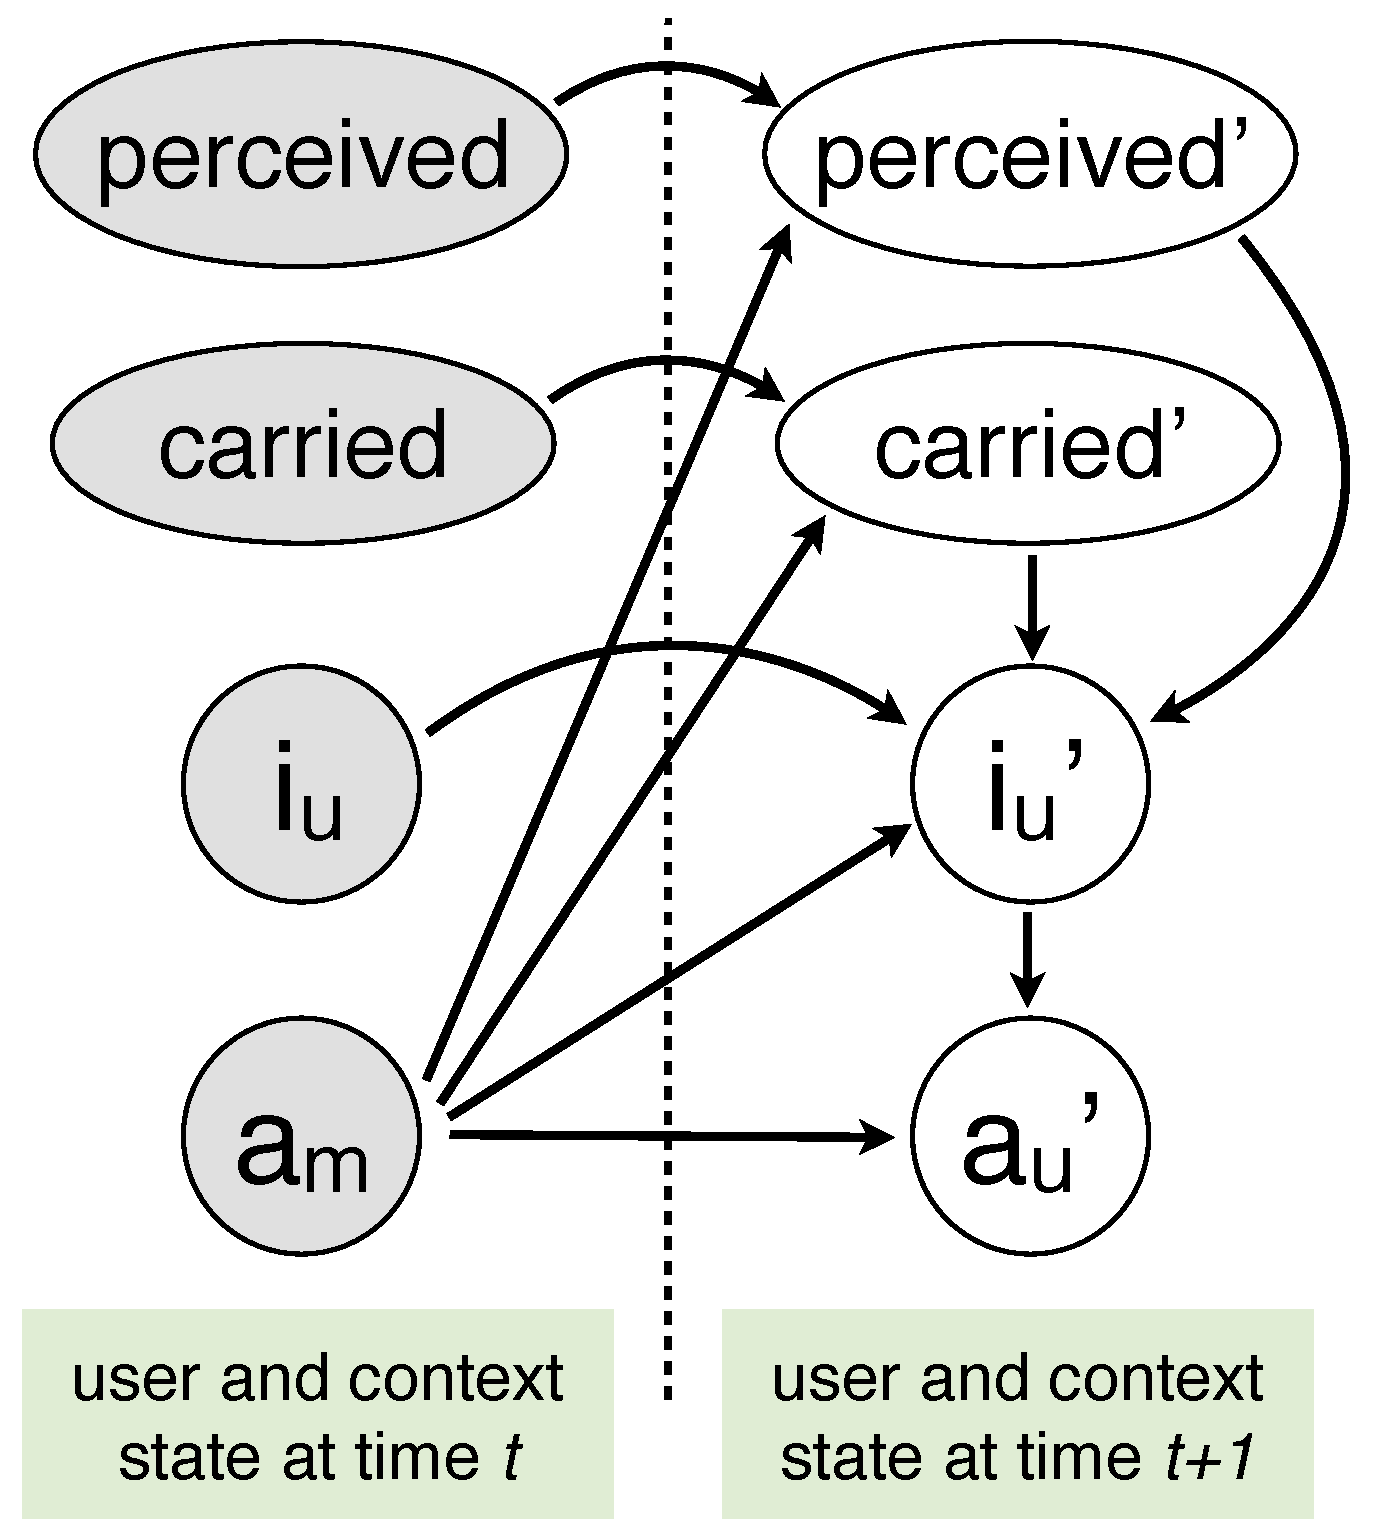
\includegraphics[scale=0.25]{imgs/simulatormodels.pdf}
\caption{User and context models employed by the simulator.}
\label{fig:simulatormodels}
\end{wrapfigure}

The resulting probabilistic model that combines these four distributions is depicted in Figure \ref{fig:simulatormodels}. The current state variables at time $t$ are greyed out, signifying that their values are observed.  It should be stressed that the knowledge of these values is limited to the simulator (since the user is aware of its own intentions and dialogue acts, and the environment ``knows'' its own state). The robot has, however, no access to the internal state of the simulator. 

The transition model was practically designed with a set of probability rules expressing the four distributions based on a small number of structural assumptions about the user behaviour.  The probabilities associated with the rule effects were then estimated by maximum likelihood on the basis of the annotated dialogues. 

\subsubsection*{Error modelling}
\index{error modelling}

In real interactions, user inputs are not directly observed by the dialogue manager but must first be processed by the speech recognition and understanding modules.  These modules are prone to various failures and frequently distort or misinterpret the actual user utterance. The user simulator should account for this fact by explicitly modelling errors and uncertainties arising from speech recognition and natural language understanding. 

In order to reproduce the imperfect nature of the communication channel, the simulator wraps every user input in an N-best list of the following form: 
\begin{equation}
\tilde{a}_u = \begin{cases} P(\text{correct } a_u) = p_1 \\ P(\text{another randomly selected value for } a_u) = p_2 \\ P(\text{spurious recognition}) = p_3 \end{cases} \nonumber
\end{equation}
where $\langle p_1, p_2, p_3 \rangle$ are probability values sampled at runtime from a three-dimensional Dirichlet distribution\index{Dirichlet distribution}.  The distribution $P(p_1, p_2, p_3)$ is estimated in an empirical manner based on actual speech recognition results for the domain. We first applied the off-the-shelf speech recogniser installed on the robot (Nuance Vocon 3200) to the audio segments corresponding to the user utterances collected in the Wizard-of-Oz study.  The recognition results were then processed in order to extract from each audio segment the three probabilities $\langle p_1, p_2, p_3 \rangle$, where $p_1$ stands for the probability of the correct utterance (which can be zero if the utterance does not appear in the N-Best list), $p_2$ to the total probability of incorrect utterances, and $p_3$ to the probability of no recognition. We finally derived a Dirichlet distribution based on these sample probabilities using the estimation method developed in \cite{minka2003}.  The particular Dirichlet distribution resulting from the recognition results was $\sim\mathsf{Dirichlet}(5.4, 0.52, 1.6)$

At runtime, the probabilities for the N-best list elements are drawn from the Dirichlet distribution. Probability values falling below a minimum threshold are automatically pruned from the N-Best list. The method has been found to match reasonably well the actual recognition results produced by the speech recogniser, although one could naturally refine the approach by e.g.\ explicitly modelling confusion probabilities between individual inputs. 

\subsubsection*{Simulation procedure}
\index{user simulator}
The simulation procedure takes the form of an interaction loop between the simulator and the dialogue system, as shown in Figure \ref{fig:exp2_architecture}.  Two separate dialogue systems are active: the simulator on the one hand and the control system for the robot on the other hand.  However, the two systems operate differently, as the simulator has a fully observable state while the system state is only partially observable.  Another obvious difference is the fact that the domain models of the system contain unknown parameters to optimise, while the simulator models are known and fixed.

Contrary to the experiments presented in the previous chapter, the dialogue architecture used in this learning experiment is essentially reduced to the dialogue management module, since the simulator and the dialogue system directly exchange their dialogue actions without needing to express them in actual spoken utterances.   

\begin{figure}[ht]
\begin{center}
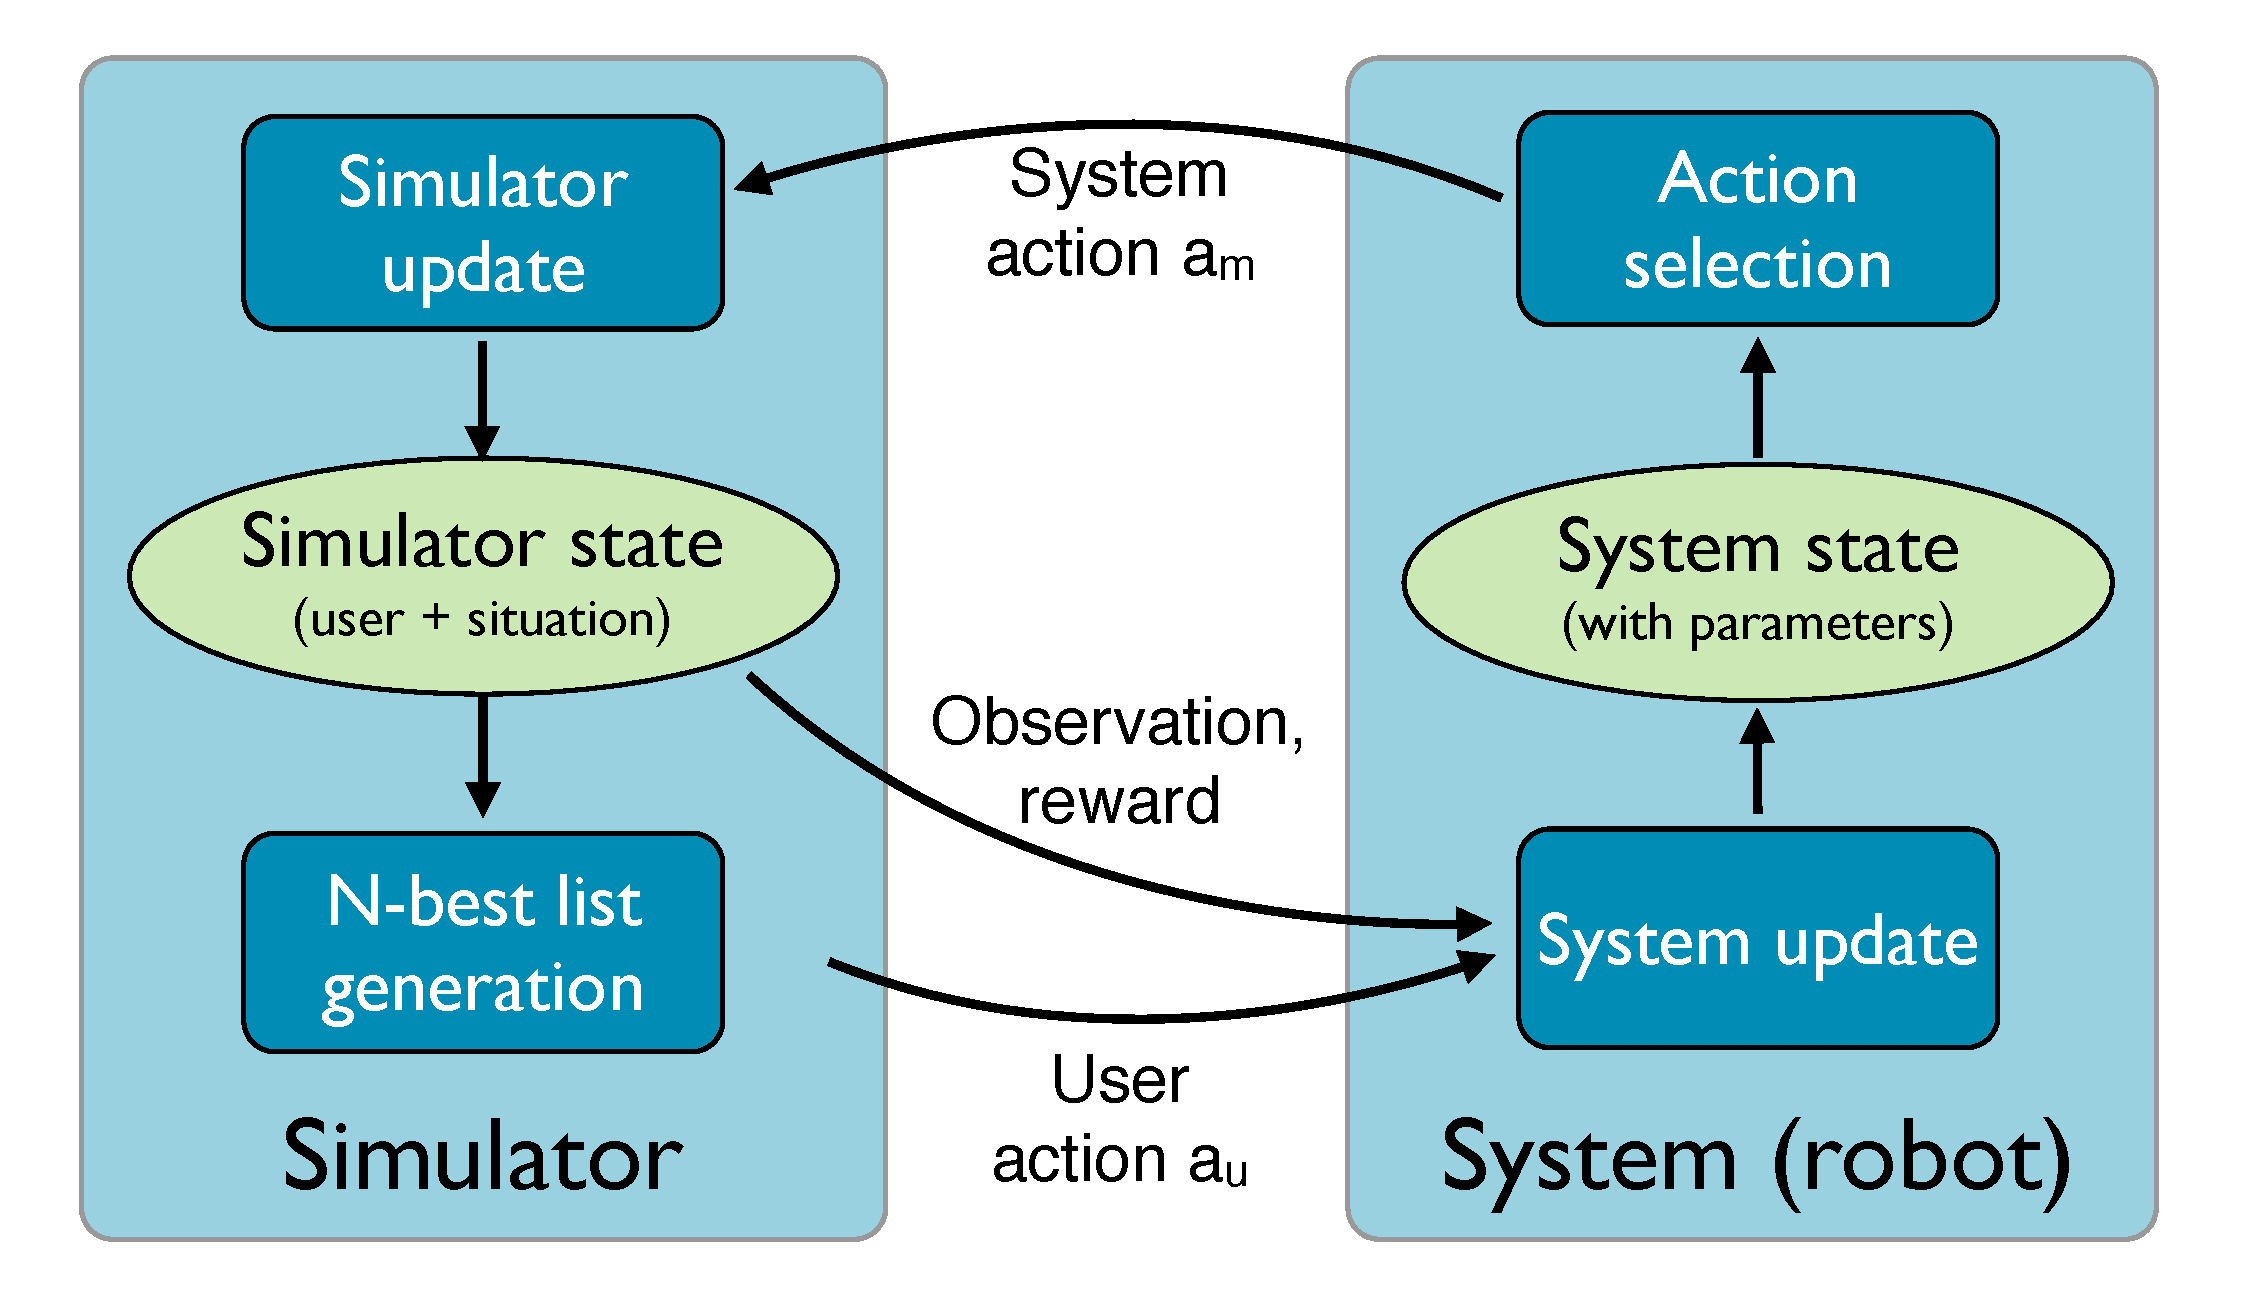
\includegraphics[scale=0.3]{imgs/exp2_architecture.pdf}
\end{center} 
\caption{Processing workflow for the simulated interaction.}
\label{fig:exp2_architecture}
\end{figure}

An example of interaction generated when coupling the simulator to the dialogue system is provided in Transcript 5. The excerpt is taken at the onset of the learning cycle, when the system's knowledge of the domain models is still rudimentary, which explains the prevalence of information-gathering actions. 

\begin{Transcript}[p!] 
\vspace{3mm}
\begin{normalsize}
$\phantom{a}$\hspace{13mm}\direct{Initial context: $\mathrm{perceived} = [\mathrm{object_1,object_2}], \mathrm{carried} = []$}
\begin{dialogue} 
\speak{Human} $\begin{bmatrix}\mathrm{Ask(PickUp(object_2))} & 0.06 \\
\mathrm{Ask(PickUp(object_1))}  & 0.42 \end{bmatrix}$ \vspace{3mm}
\speak{Robot} \ $\mathrm{AskRepeat}$ \hspace{47mm} $\rightarrow \mathrm{Reward} = -1$ \vspace{3mm}
\speak{Human} $\begin{bmatrix}\mathrm{Ask(DoYouSee(object_2))}  & 0.01 \\ 
\mathrm{Ask(PickUp(object_1))} & 0.77 \end{bmatrix}$ \vspace{3mm}
\speak{Robot} \ $\mathrm{Ground(PickUp(object_1))}$ \hspace{21mm} $\rightarrow \mathrm{Reward} = 2$ \vspace{3mm}
\speak{Robot} \ $\mathrm{Do(PickUp(object_1))}$ \hspace{29mm} $\rightarrow \mathrm{Reward} = 6, \mathrm{carried} = [\mathrm{object_1}]$ \vspace{3mm}
\speak{Human} $\begin{bmatrix}\mathrm{Ask(DoYouSee(object_2))} & 0.05 \end{bmatrix}$ \vspace{3mm}
\speak{Robot} \ $\mathrm{AskRepeat}$ \hspace{47mm} $\rightarrow \mathrm{Reward} = -1$ \vspace{3mm}
\speak{Human} $\begin{bmatrix} \mathrm{Ask(DoYouSee(object_2))}  & 0.87 \end{bmatrix}$ \vspace{3mm}
\speak{Robot} \ $\mathrm{AskConfirm(DoYouSee(object_2))}$ \hspace{7mm} $\rightarrow \mathrm{Reward} = -0.5$ \vspace{3mm}
\speak{Human} $\begin{bmatrix}\mathrm{RepeatLast} & 0.05 \\ \mathrm{Confirm} & 0.63 \end{bmatrix}$ \vspace{3mm}
\speak{Robot} \ $\mathrm{ConfirmDetection}$ \hspace{34mm} $\rightarrow \mathrm{Reward} = 6$ \vspace{3mm}
\speak{Human} $\begin{bmatrix}\mathrm{Ask(Move(Forward))} & 0.73 \\
\mathrm{Ask(PickUp(object_2))}& 0.03 \end{bmatrix}$ \vspace{3mm}
\speak{Robot} \ $\mathrm{AskRepeat}$ \hspace{47mm} $\rightarrow \mathrm{Reward} = -1$ \vspace{3mm}
\speak{Human} $\begin{bmatrix}\mathrm{Ask(Move(Forward))} & 0.92 \\
\mathrm{Ask(Move(Left))} & 0.04 \end{bmatrix}$ \vspace{3mm}
\speak{Robot} \ $\mathrm{Ground(Move(Forward))}$ \hspace{22mm} $\rightarrow \mathrm{Reward} = 2$ \vspace{3mm}
\speak{Robot} \ $\mathrm{Do(Move(Forward))}$ \hspace{31mm} $\rightarrow \mathrm{Reward} = 6$
\end{dialogue}
$\phantom{a}$\hspace{13mm}\direct{...} \vspace{3mm}
\end{normalsize}
\caption{Example of simulated interaction}
\end{Transcript}

\subsection{First experiment}

The goal of the first experiment is to determine whether the use of probabilistic rules has a beneficial influence on the learning performance\index{learning performance} of the agent. The motivation is sensibly the same as the one put forward in the experiment of the previous chapter, except that the estimation procedure is here based on model-based Bayesian reinforcement learning techniques instead of supervised learning. 

The experiment focuses more specifically on the statistical estimation of the transition model\index{transition model} for the human--robot interaction domain described in Section \ref{sec:exp2_dd}. Based on the simulator presented in the previous pages, the experiment compares two alternative representations of the transition model: one baseline model encoded via standard categorical distributions, and one equivalent model encoded via probability rules.  The relative performance of these two representations is measured by the average return -- i.e.\ the sum of rewards -- per interaction. 

The reward model\index{reward model} was held fixed and identical in both cases (cf. Table \ref{table:rewards}). Online planning\index{online planning} was used for action selection and operated with a horizon of length 2. In other words, the planner looked ahead one step into the future to determine the effects of its actions.  

%The planner included an observation model introducing random noise to the user dialogue acts.



\subsubsection*{Baseline model}
\index{factored probabilistic model}

The transition model $P(s'\, | \, s, a_m)$ is represented in the baseline approach through traditional factored categorical distributions. More precisely, the transition model is divided into a user goal model $P(i_u'\, | \, i_u, a_m)$ and a user action model $P(a_u' \, | \, i_u',a_m)$.\footnote{The two contextual variables $\mathrm{perceived}$ and $\mathrm{carried}$ are not included in the transition model since their values do not need to be predicted in advance.} The user goal model is defined in the following manner:
\begin{equation}
P(i_u' \, | \, i_u, a_m) = \begin{cases}
P(i_u') & \text{if } a_m \text{ fullfils the intention } i_u \\
1 & \text{if above condition does not hold and } i_u' = i_u \\
0 & \text{otherwise} \end{cases} \nonumber
\end{equation}
where $P(i_u')$ is a categorical distribution that expresses the prior probability of a new user intention $i_u'$. The user action model $P(a_u' \, | \, i_u',a_m)$ is for its part constructed as a plain probability table where each possible assignment of values for the parent variables $i_u'$ and $a_m$ is assigned a distinct categorical distribution on the values of $a_u'$. 

The resulting parameters for these categorical distributions are encoded with Dirichlet priors.  The baseline model used for this experiment contains a total of 229 Dirichlet parameters, composed of one Dirichlet with 12 dimensions and 228 with 16 dimensions.  Weakly informative priors are used to initialise the prior distributions.\index{parameter priors}

A linear model\index{linear model} has also been constructed for this experiment but is not shown in the results as its parameter estimation systematically diverged and fared much worse that the classical factored distributions, most likely due to the non-linearity of the underlying domain models. 


\subsubsection*{Rule-structured model}
\index{rule-structured model}

The rule-structured model is encoded with parametrised probability rules. A total of six rules with 13 corresponding Dirichlet parameters (of varying dimensions) is used to define the transition model.   As for the baseline model, the rule parameters are initially associated with weakly informative Dirichlet priors.\index{parameter priors}  The rules designed for the experiment are listed in Appendix \ref{chap:domainspecs}.

\subsubsection*{Empirical results}

The performance was first measured in terms of average return\index{average return} per simulated interaction, shown in Figure \ref{fig:return_exp21}.  To analyse the accuracy of the transition model, we also derived the Kullback--Leibler divergence\index{Kullback--Leibler divergence} \citep{KLDIVERGE} between the next user act distribution $P(a_u')$ predicted by the learned model and the actual distribution followed by the simulator at a given time, as shown in Figure \ref{fig:divergence}.   Some residual discrepancy is to be expected between these two distributions, the latter being based on the actual user intention while the former must infer it from the current belief state. The results of both figures are averaged on 100 simulations.

\begin{figure}[p]
\centering
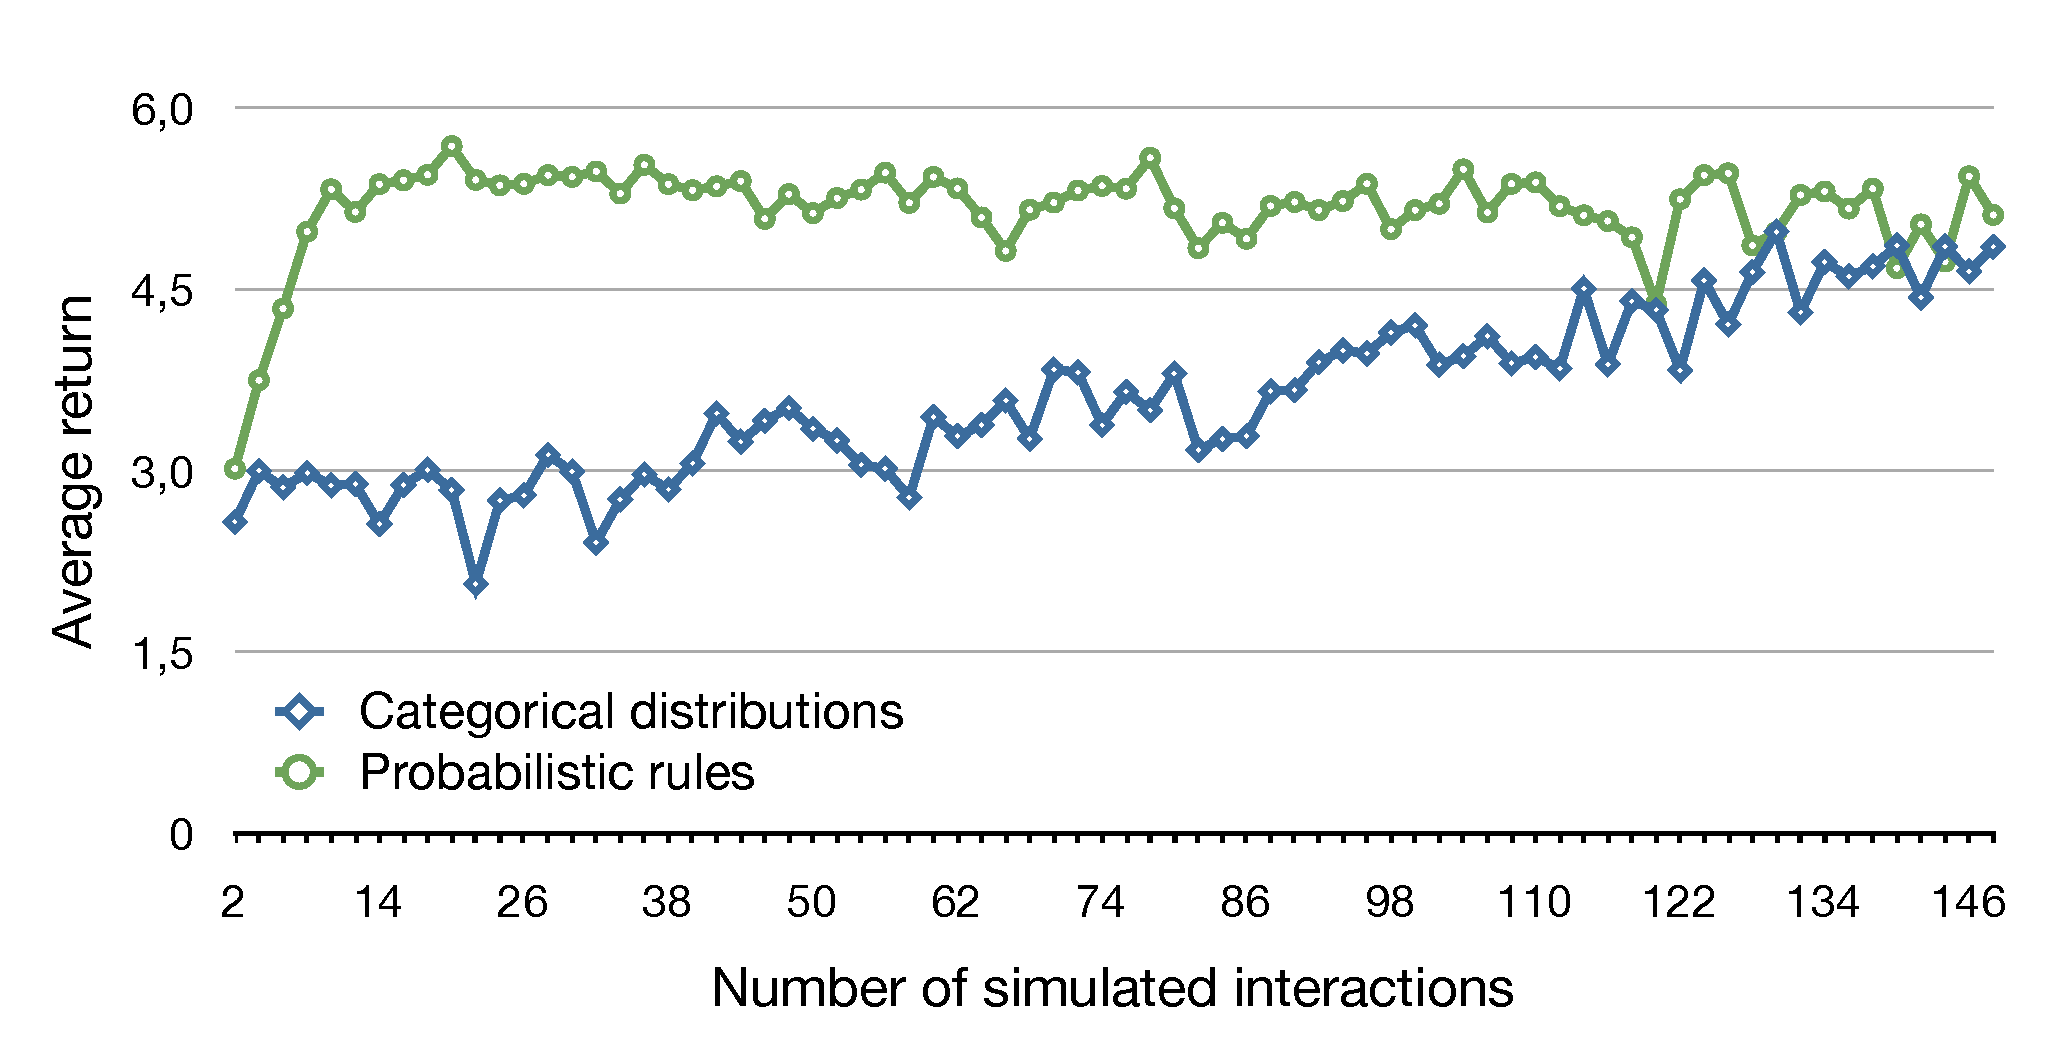
\includegraphics[scale=0.42]{imgs/return_exp21.pdf}
\caption{Average return as a function of the number of simulated interactions.}
\label{fig:return_exp21}
\end{figure}

\begin{figure}[p] 
\begin{center}
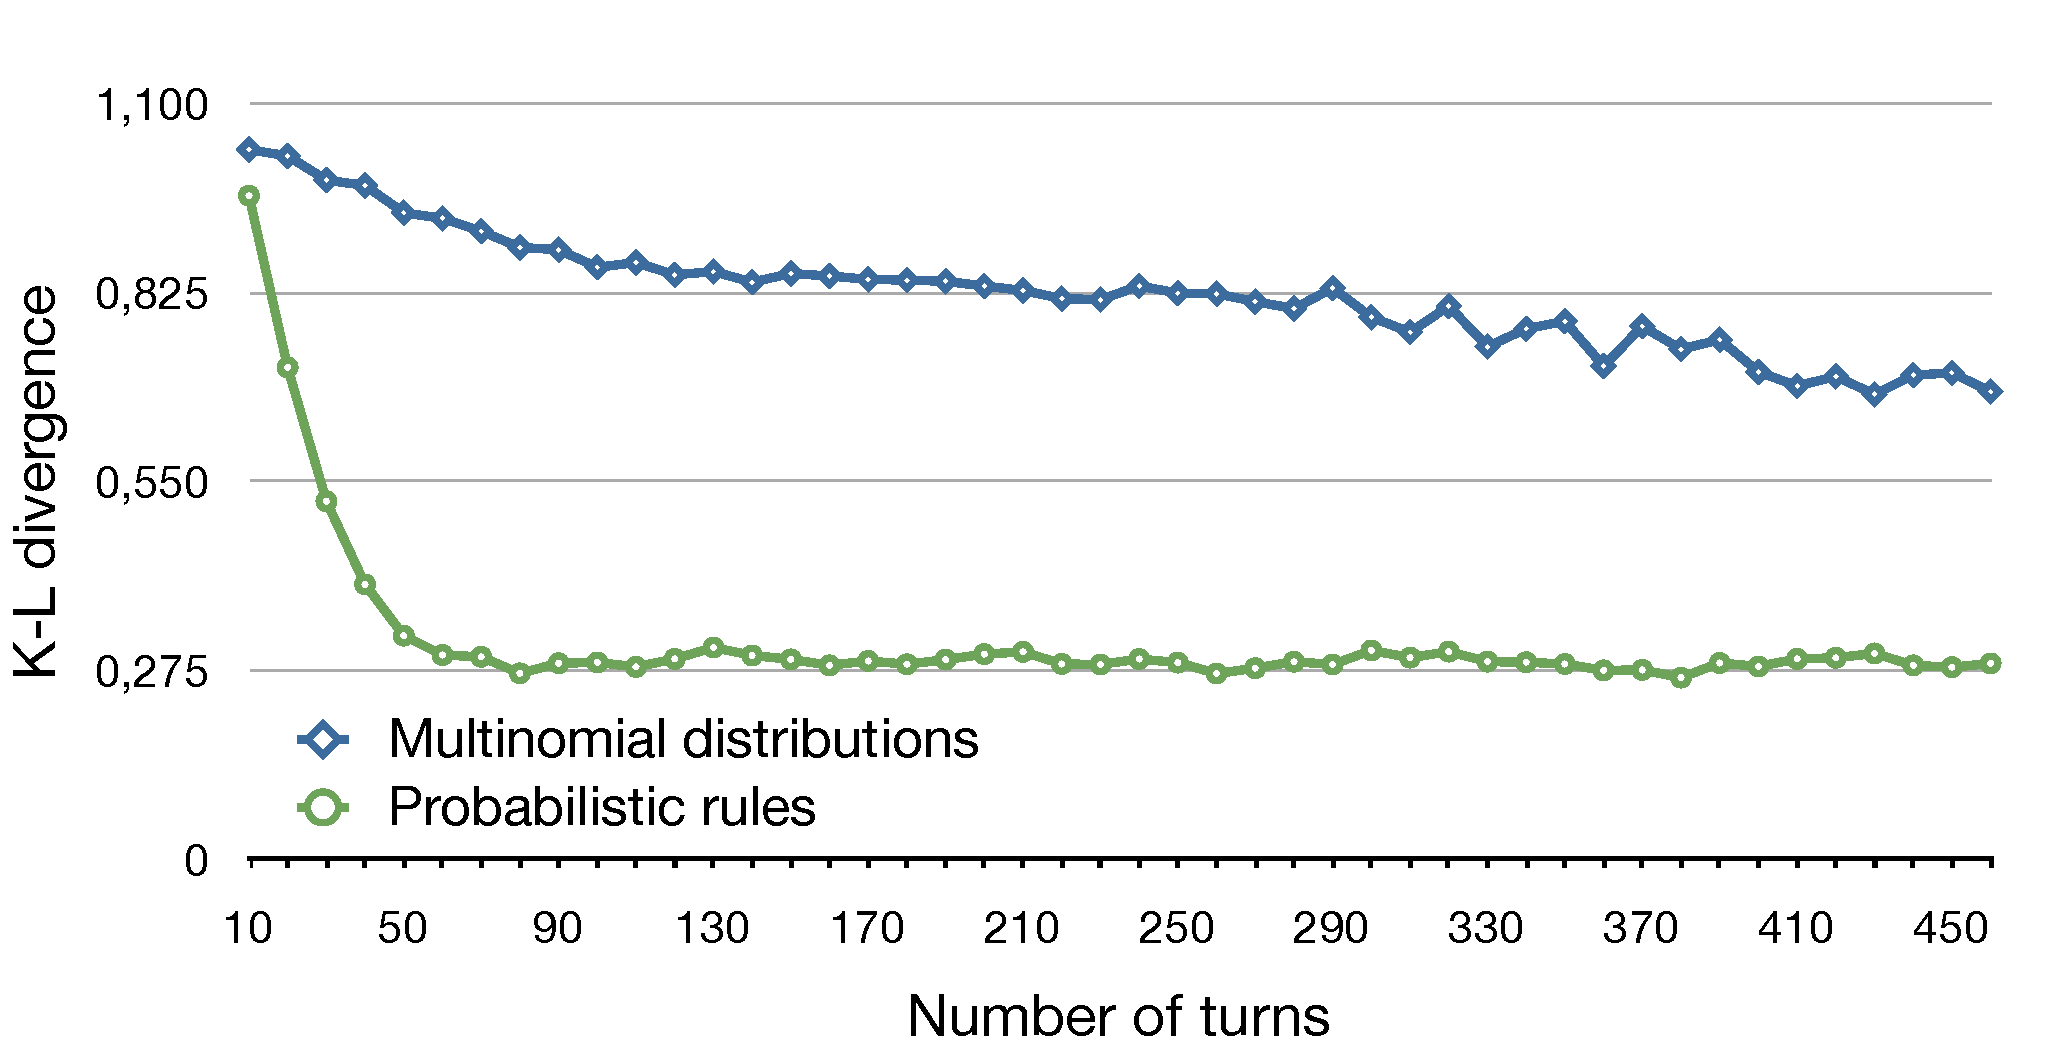
\includegraphics[scale=0.42]{imgs/kldivergence.pdf}
\end{center} 
\caption{Kullback--Leibler divergence between the distribution $P(a_u')$ estimated from the current model and the actual distribution followed by the simulator.}
\label{fig:divergence}
\end{figure}

\subsubsection*{Analysis of results}

The empirical results illustrate that both models are able to capture at least some of the interaction dynamics and achieve higher returns as the number of turns increases, but they do so at different learning rates.  In our view, this difference is to be explained by the higher generalisation capacity\index{generalisation capacity} of the probabilistic rules compared to the unstructured categorical distributions.  

One can observe from the empirical results that the Dirichlet parameters associated with the probabilistic rules converge to their optimal value very rapidly, after a handful of episodes.  This is a promising result, since it implies that the proposed approach could in principle optimise dialogue policies from live interactions, without resorting to a user simulator.

One caveat is nevertheless worth mentioning here.  As described in the previous section, the simulation model used to sample the next intentions and actions of the user is built on a number of structural assumptions.  The learning results must therefore be interpreted with caution, as one could object that the good learning performance of the rule-structured model is an artefact of the regular behaviour exhibit by the simulator, and that such regularities may not be found in messy, real-world dialogues. This is a valid objection, although the posited assumptions on the user behaviour are relatively conservative and backed by a preliminary analysis of the actual user responses in the Wizard-of-Oz studies. However, we shall see in Chapter \ref{chap:user-evaluation} that the promising results presented here also carry over to genuine interactions conducted without a simulator. 

\subsection{Second experiment}
\label{rrlearning-exp22}

The first experiment was confined to the analysis of model-based methods to reinforcement learning and did not compare the performance of model-based and model-free approaches to the estimation of rule parameters.  This second experiment remedies this shortcoming. As in the previous experiment, the reward model is provided but the transition model is unknown.  Both approaches are encoded in this experiment with probabilistic rules.

In the model-free case, the rule parameters encode the action--value model $Q(s,a)$ over the return of state--action pairs, while the model-based case focuses on the transition model $P(s'\, | \, a,s)$.  Figure \ref{fig:exp22_comparison} illustrates these two learning strategies.  

\begin{figure*}[ht]
\subfigure[Model-based approach]{
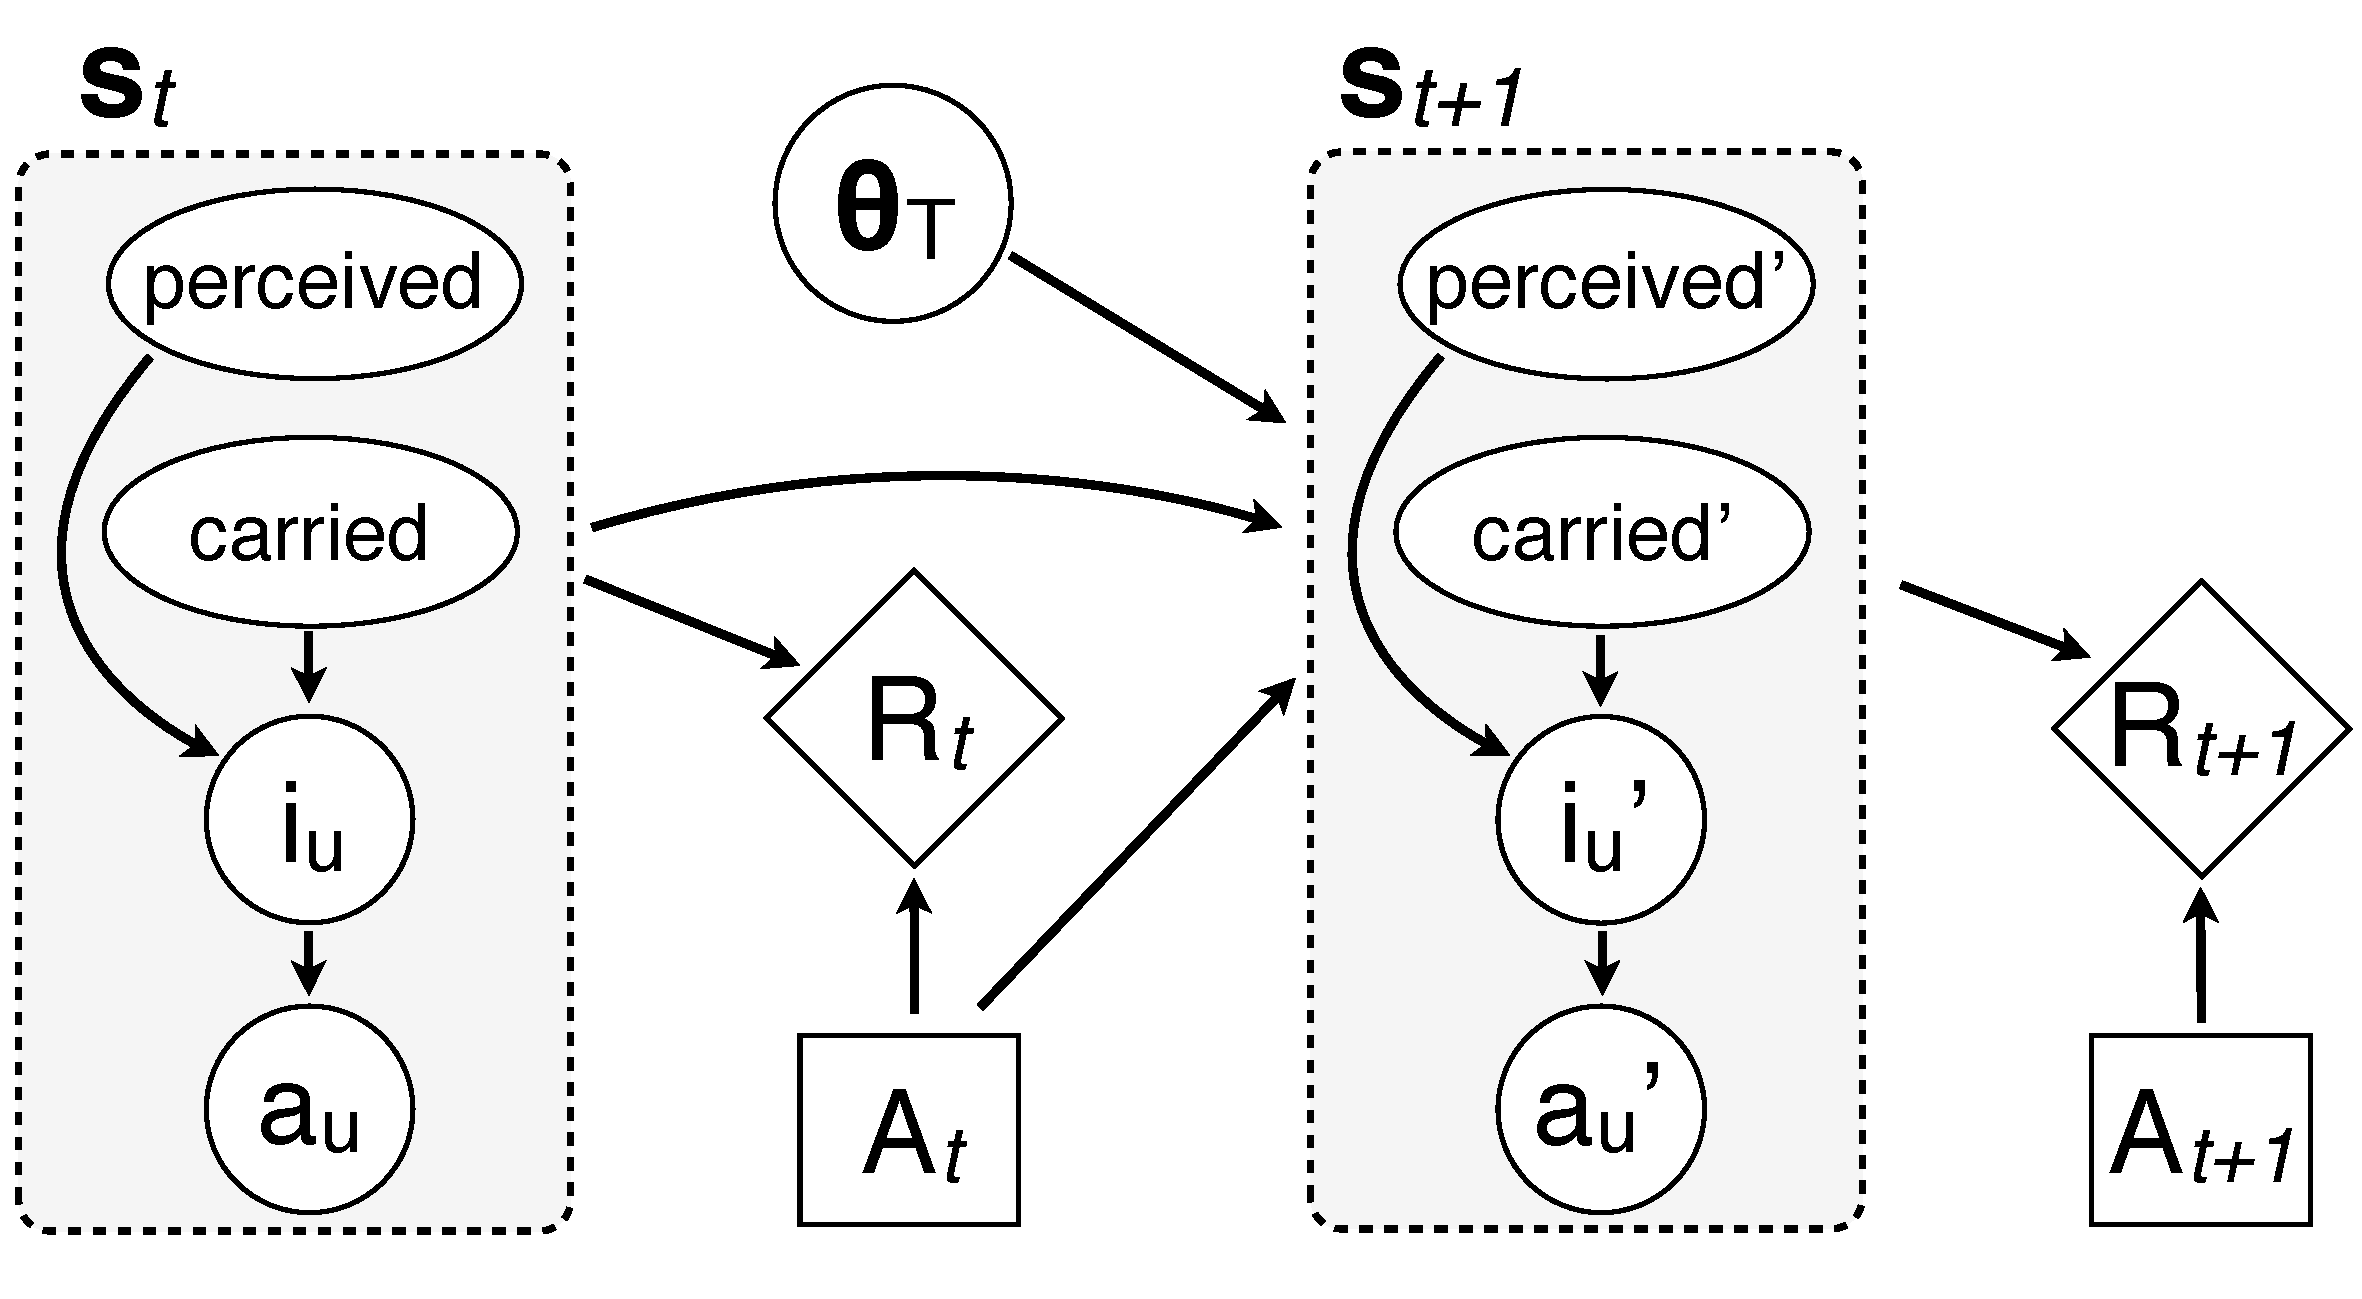
\includegraphics[scale=0.23]{imgs/diagram_modelbased_exp22.pdf}
} \hspace{16mm} \subfigure[Model-free approach]{
\centering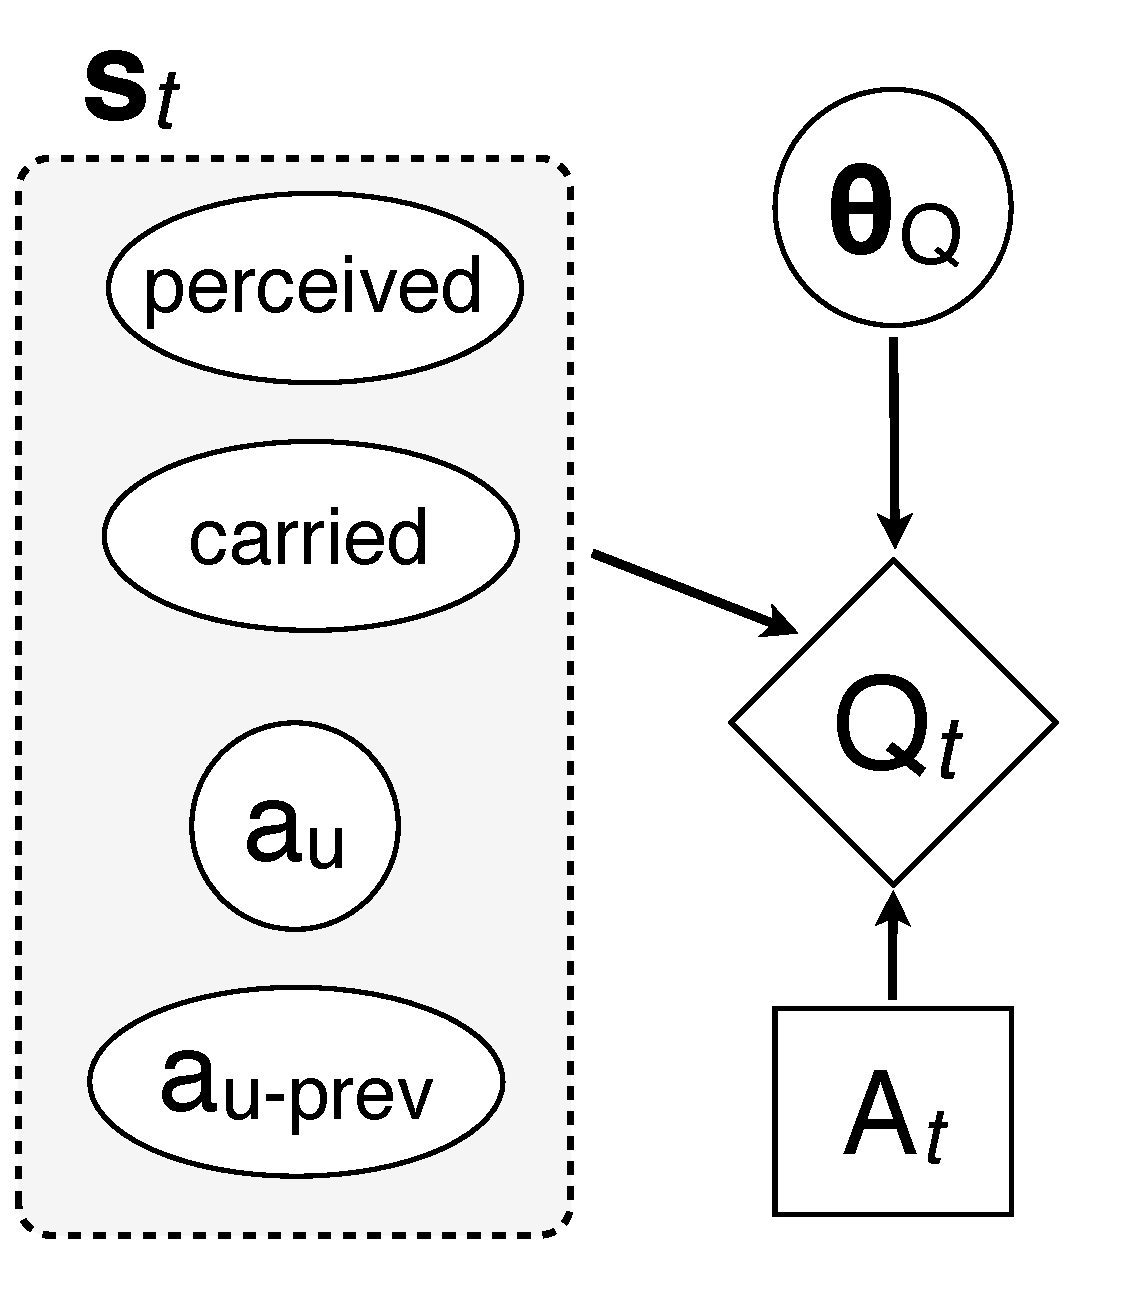
\includegraphics[scale=0.23]{imgs/diagram_modelfree_exp22.pdf}
}
\caption{Model-based (left) and model-free (right) approaches compared in the experiment.}
\label{fig:exp22_comparison}
\end{figure*}


\subsubsection*{Model-based approach}
\index{rule parameters!model-based RL of}

The model-based approach is identical to the one presented in the previous experiment. The transition model is thus structured with six rules associated with 13 corresponding Dirichlet parameters of varying dimensions.   The Dirichlet parameters are again initialised with weakly informative Dirichlet priors.  As for the first experiment, the action selection was performed with an online planner operating with a horizon of 2. 

\subsubsection*{Model-free approach}
\index{rule parameters!model-free RL of}

The model-free approach relied on a utility model structured with 12 probabilistic rules associated with 27 Gaussian parameters. As no transition model is here available to infer the underlying user intentions, the dialogue state is defined on the basis of the recent history of dialogue acts, namely the last user action $a_u$, last system action $a_m$ and preceding action $a_{u\mbox{-}prev}$. The dialogue state also included the list of objects currently perceived and carried by the robot.

The resulting rule parameters were optimised using the SARSA-based method outlined in Section \ref{sec:modelfree}. 

\subsubsection*{Empirical results}

The simulator was coupled to the dialogue system to compare the learning performance of the two methods.  Figure \ref{fig:return_episodes} shows the average returns over 100 iterations.

\begin{figure}[p]
\centering
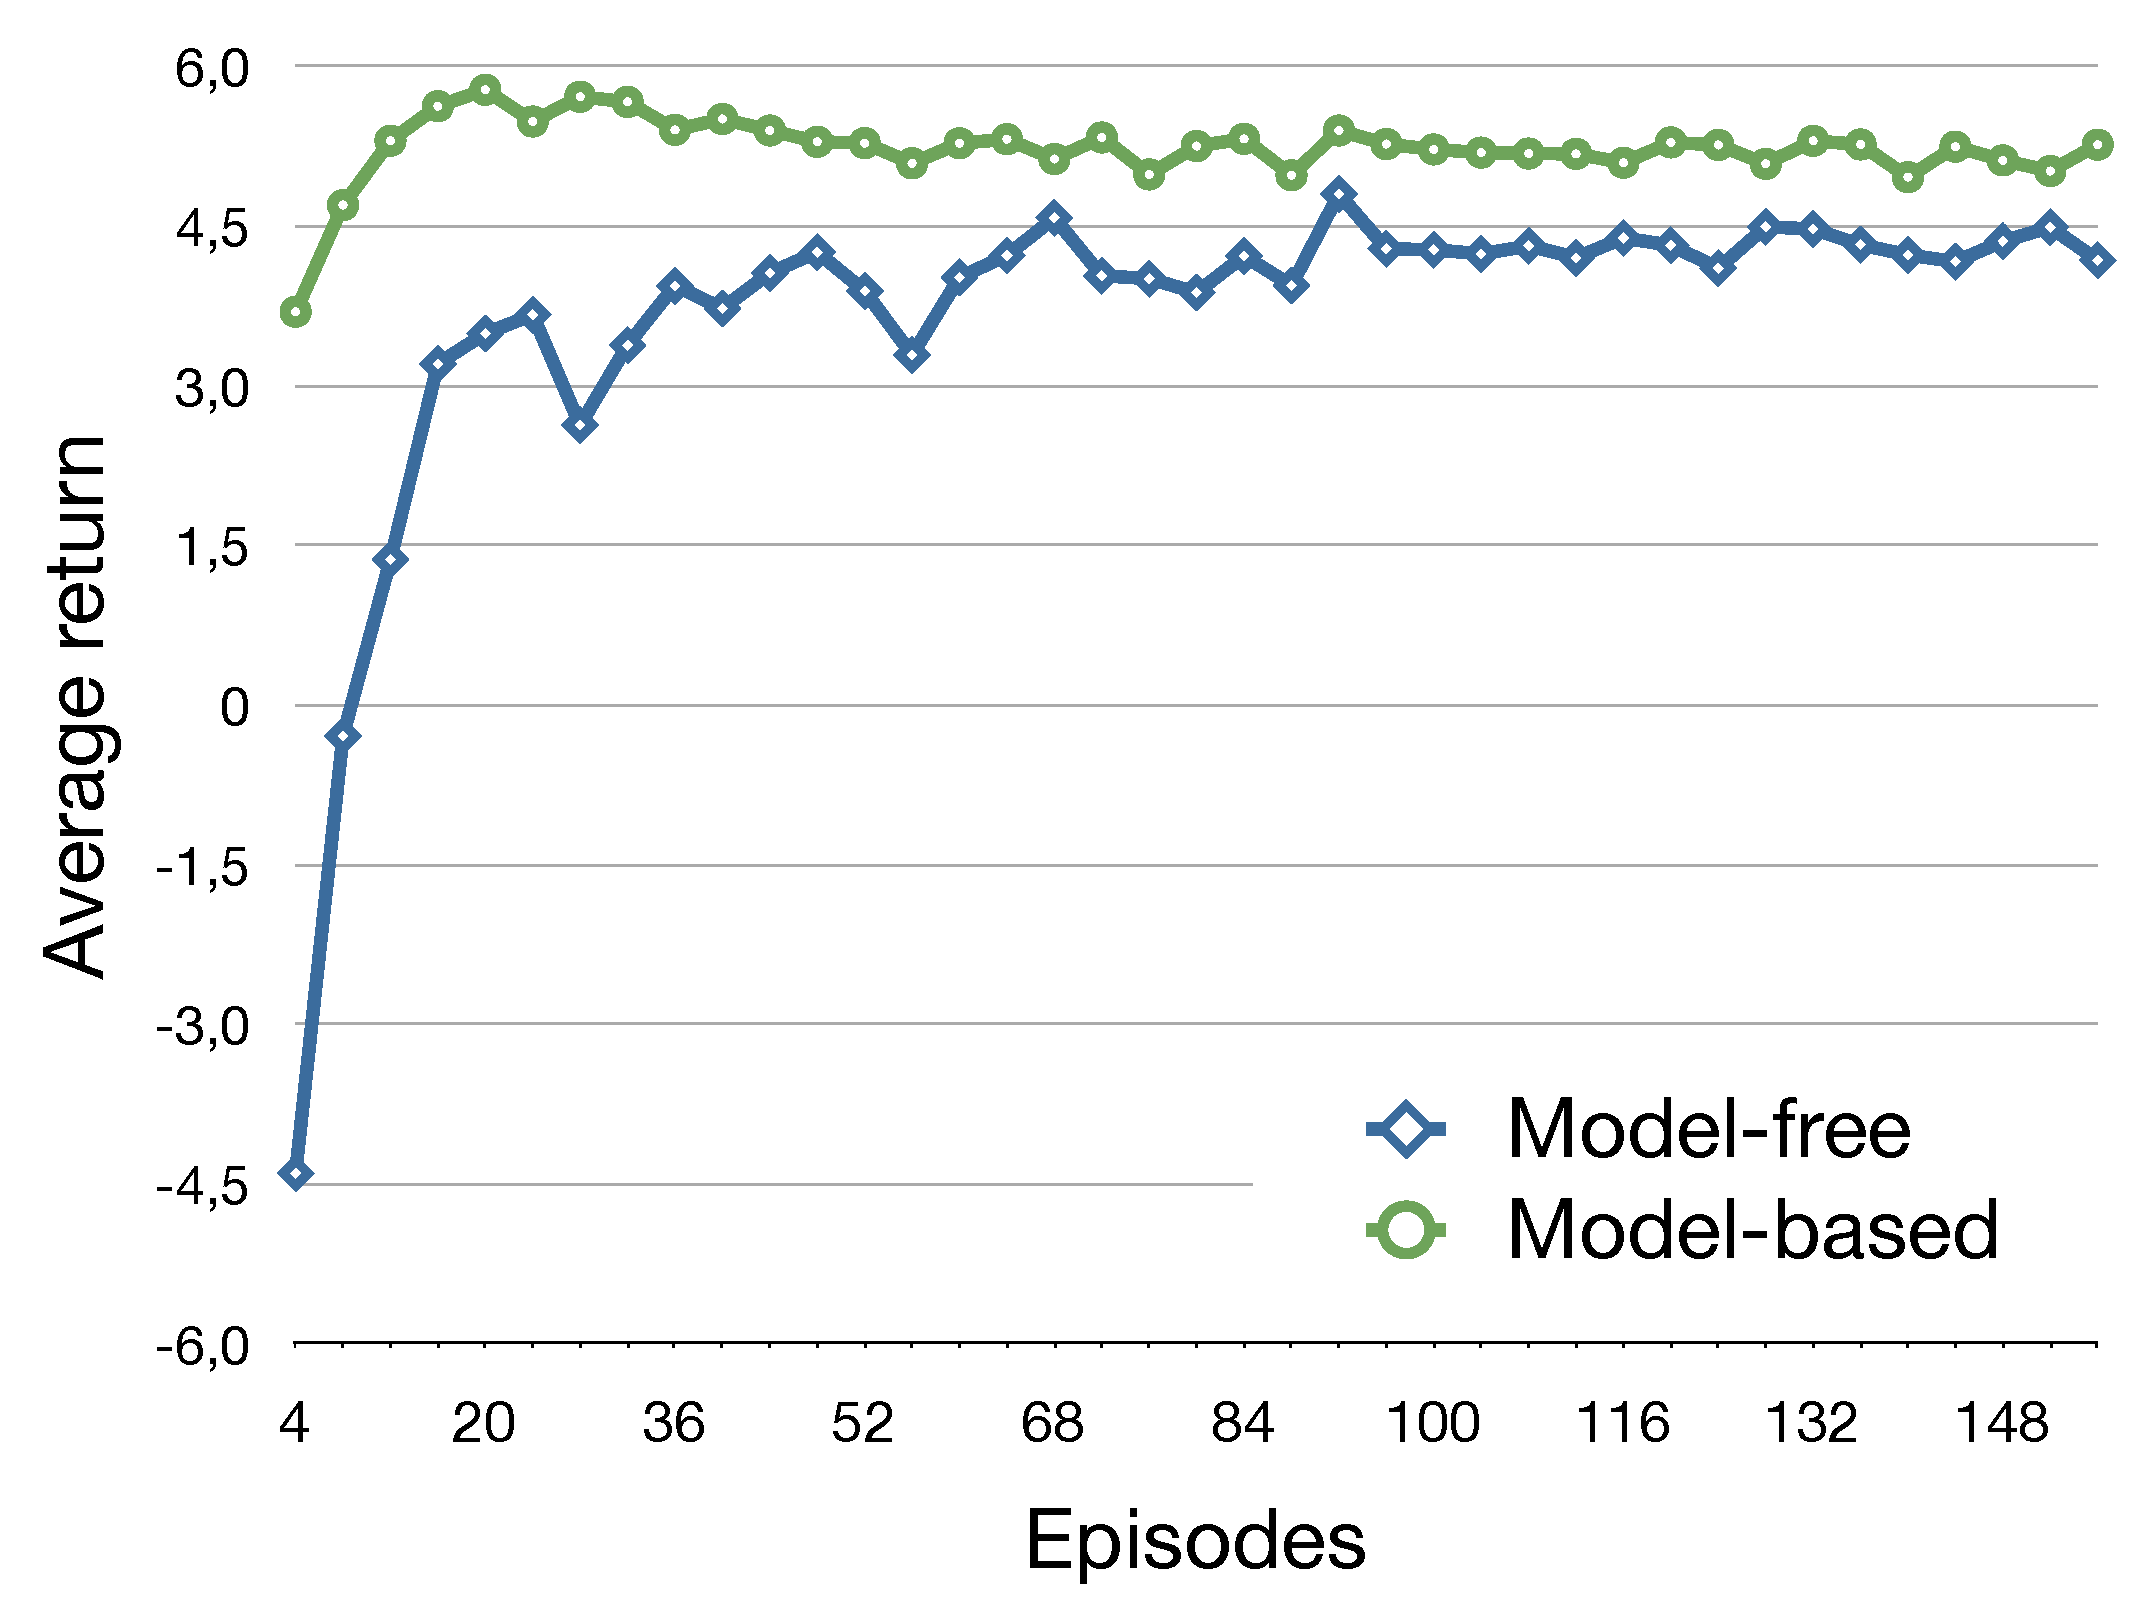
\includegraphics[scale=0.42]{imgs/episodes.pdf}
\caption{Average return as a function of the number of episodes.}
\label{fig:return_episodes}
\end{figure}

\begin{figure}[p]
\centering
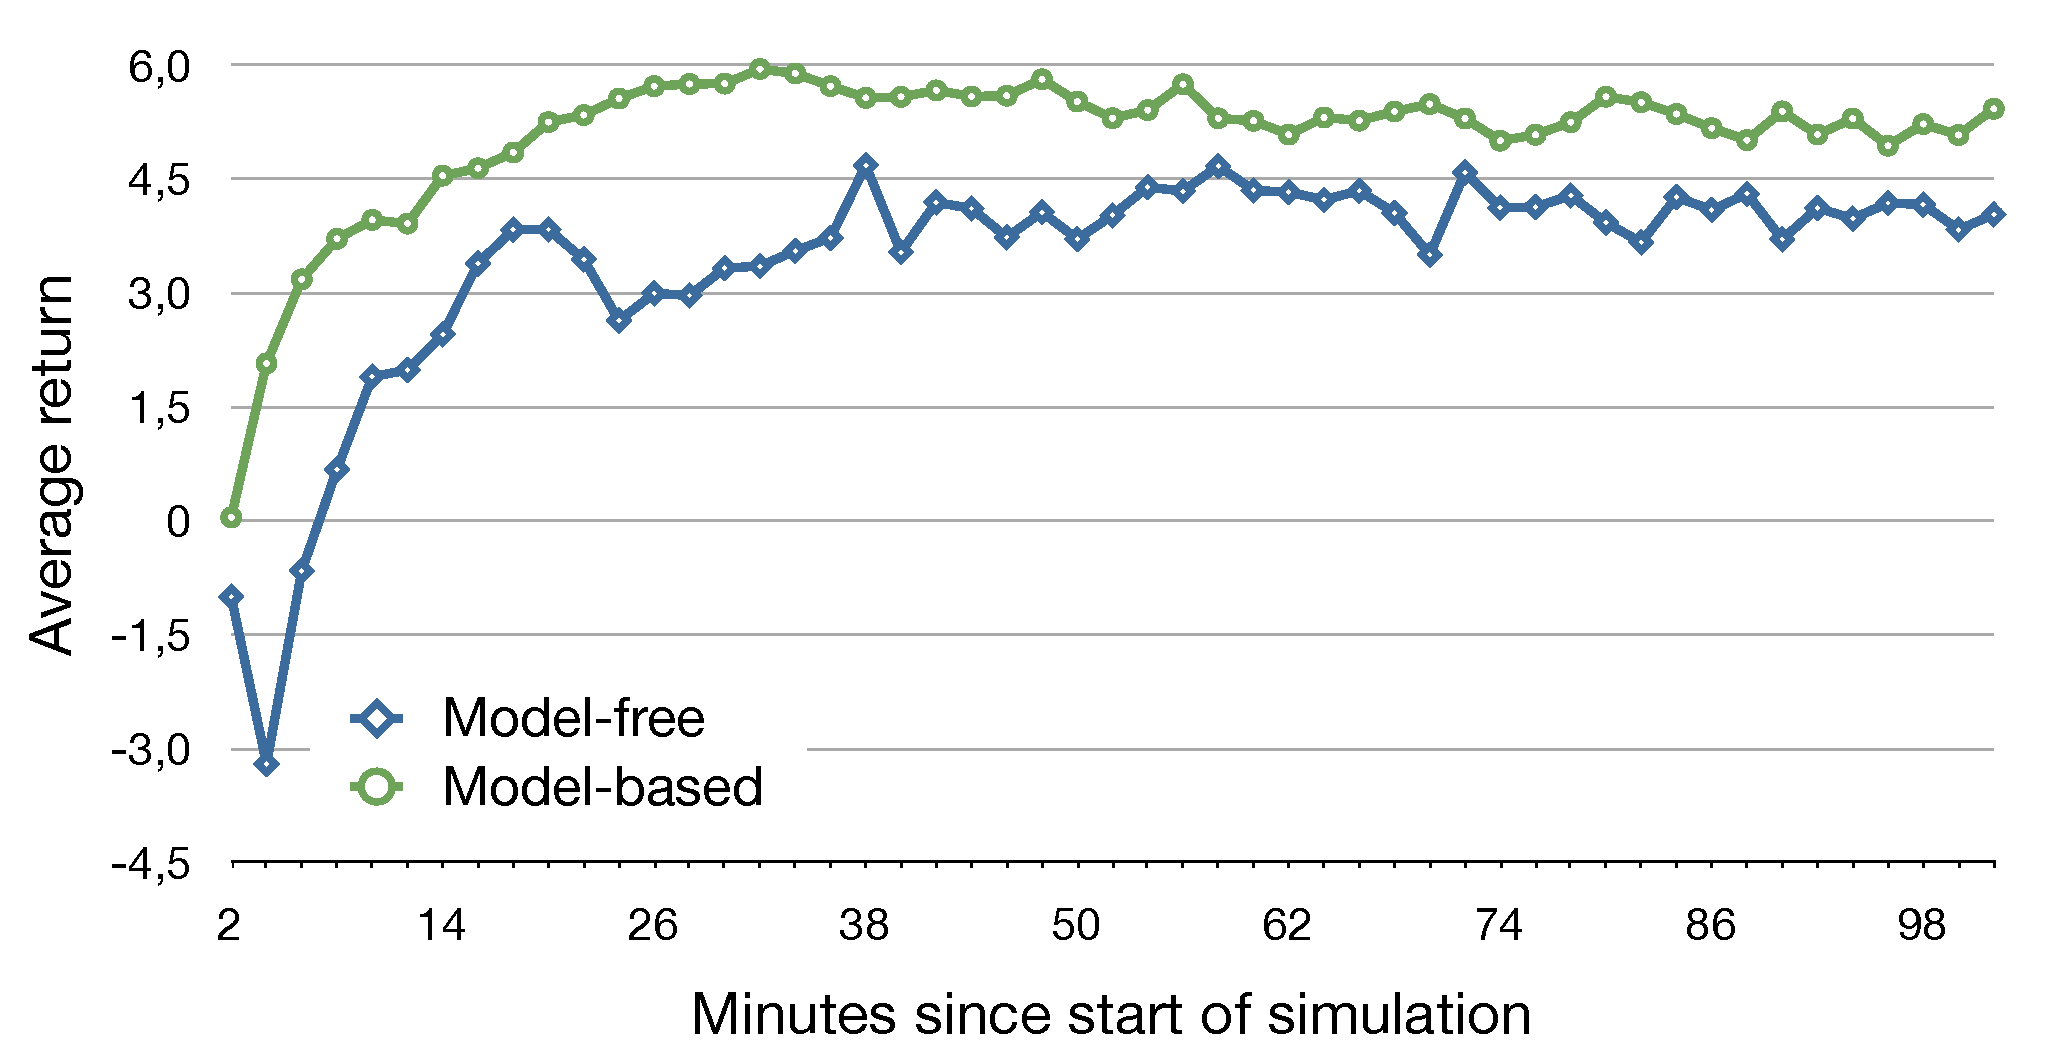
\includegraphics[scale=0.42]{imgs/timing.pdf}
\caption{Average return as a function of the elapsed time.}
\label{fig:return_time}
\end{figure}

\subsubsection*{Analysis of results}

We can notice on Figure \ref{fig:return_episodes} that the model-based approach converges to a high-quality policy in fewer episodes than its model-free counterpart.  However, this performance comes at the cost of higher computational demands brought about by the need to perform online planning, as evidenced in Figure \ref{fig:return_time} by the roughly similar times required for convergence (around 50 min.). We can also observe that the model-based approach yields slightly higher returns in this experiment, although this difference is harder to explain.  One hypothesis is that the model-based approach can accumulate evidence about the underlying user intention in its belief state, while its model-free equivalent lacks an explicit transition model and can therefore only ground its decisions on the history of dialogue acts and objects perceived by the robot.

The results suggest that the model-based approach outperforms its competitor in this type of learning contexts. However, this conclusion warrants some cautionary remarks.   First, the tractability of the model-based approach is directly dependent on the length of the planning horizon. Domains with longer horizons might be better addressed with a model-free strategy due to the exponential growth of the search tree. Second, the model-free learning algorithm presented here remains relatively simple -- as it is based on a Bayesian variant of the well-known SARSA algorithm -- and more recent frameworks such as Gaussian processes\index{Gaussian processes} \citep{milica2013} might improve the model-free results. Finally, it should be noted that the model-based method could rely in this work on the availability of the reward model. This is not an unreasonable assumption for dialogue domains, as the reward model is often a reflection of the application objectives as specified by the system designer. It may nevertheless be difficult to specify all aspects of the reward model at design time. Whether the results carry out to cases where the reward model must also be (partially or fully) estimated remains an open question.

The model-free approach presented in this experiment only focused on the estimation of the action--value model and did not include a transition model.  An interesting idea for future work would be to blend the two optimisation methods and simultaneously estimate a transition model together with the action--value model.  Such a hybrid approach would combine the advantages of model-free and model-based strategies, since it would allow the action--value model to be grounded in high-level variables such as the user intentions instead of remaining confined to observation variables. In this hybrid framework, action selection could be performed via a mixture of offline and online planning as in \cite{RossC07}. 

\section{Conclusion}

%As in other areas of machine learning, Bayesian techniques are becoming increasingly popular in reinforcement learning. 

This chapter has introduced two alternative Bayesian reinforcement learning techniques to the optimisation of parameters associated with probabilistic rules.

The first technique is a model-based approach that explicitly constructs statistical models of the domain in the form of transition, observation and reward models.  The range of possible values for the domain parameters are represented as prior probability distributions that are incrementally updated based on the observations and rewards perceived during the interactions. Action selection is achieved through forward planning on the basis of the current dialogue state and domain parameters. Probabilistic rules are employed to structure the domain models and thereby reduce the number of parameters to optimise. 

The second technique is a model-free approach that skips the estimation of the domain models in order to directly construct an action--value model expressing the $Q$-values of state--action pairs.  As these $Q$-values are never directly observed, their estimation is bootstrapped on the basis of Bellman's equation. We described how the action--value model could also be structured with utility rules and optimised through a Bayesian variant of the SARSA learning algorithm combined with $\epsilon$-greedy action selection. 

The last section presented two learning experiments conducted in a simulated environment.  The simulator was common to both experiments and constructed on the basis of a preliminary Wizard-of-Oz study carried out in a human--robot interaction domain. The simulator included three distinct models, all estimated from the collected Wizard-of-Oz data: a \textit{user model} expressing how the user intentions and dialogue acts are likely to evolve as a function of the system actions, a \textit{context model} expressing the objects in the visual field of the robot as well as the ones carried by the robot, and an \textit{error model} introducing errors and inaccuracies into the generated user input in order to mimic the imperfect nature of speech recognition.

On the basis of this simulator, the first experiment compared the performance of model-based Bayesian reinforcement learning on two alternative formalisations of the transition model.  The first formalisation relied on traditional factored distributions, while the second represented the transition model through probability rules. The empirical results showed that the rule-structured model could converge to a high-performing dialogue behaviour -- as measured by the average return per interaction -- much faster than the baseline.

The second experiment examined the relative performance of model-based and model-free approaches.  The two models compared in this experiment were structured with probabilistic rules. The results showed that the model-based approach fared slightly better than its model-free counterpart in terms of average return per interaction.  However, we noted that this difference was contingent on particular aspects of the experimental setup such as the length of the planning horizon and the prior availability of a reward model. 

The previous and present chapter demonstrated how probabilistic rules can facilitate the optimisation of dialogue policies both in the supervised and reinforcement learning case. The experiments have nevertheless so far concentrated on the \textit{learning performance} of rule-structured approaches, and have not yet evaluated the effects of probabilistic rules on practical measures of interaction quality and user satisfaction. Chapter \ref{chap:user-evaluation} will address this important question. But before doing so, we first discuss the technical implementation of the data structures and algorithms exposed in this thesis. This is the subject of the next chapter.

\chapter{User experiments}


\chapter{Concluding remarks}
\label{chap:conclusions}

\section{Summary of contributions}

\note{be able to capture richer conversational context, and better account for the cooperative nature of dialogue (e.g. Jokinen's argument against classical utility maximisation approaches).}

\section{Future work}

\note{Formally characterise the expressivity of the rules and extend them to handle Ginzburg style update rules?}

\note{more complex domains, with more variables and more complex dynamics}

\note{Try to learn a policy in a fully online fashion with real users, without simulator}

\note{do online reinforcement learning with real users and combine imitation+reinforcement learning}

\note{joint optimisation of models}


\appendix

\chapter{Implementation}
\label{chap:opendial}
\index{openDial@\opendial{}|textbf}

This chapter outlines the most important features of the \opendial{} toolkit.\footnote{The name of the toolkit was chosen because of the open design that characterises the framework, and more particularly its extensible, domain-independent architecture with a declarative domain specification.} \opendial{} is a Java-based software toolkit developed to construct and evaluate dialogue systems based on probabilistic rules. The toolkit aims to be fully generic and domain-independent, since all domain-specific knowledge is captured in the declarative specification\index{dialogue domain!declarative design of} of the dialogue domain.

The toolkit implements all the data structures and algorithms detailed in this thesis and served as a experimental platform to carry out the empirical studies presented in Chapters \ref{chap:wozlearning}, \ref{chap:rllearning} and \ref{chap:user-evaluation}. Dedicated components have been developed to interface \opendial{} with the Nao robotic platform and adapt the architecture to human--robot interaction settings.

The chapter is divided in two sections.  The first section focuses on the design of the \opendial{} toolkit and describes its general workflow, the specification of dialogue domains in XML, and the concrete implementation of the algorithms employed for approximate inference, sampling and forward planning. We also briefly compare the toolkit to other available architectures and discuss its current technical limitations.  The second section goes on to explain how the toolkit is integrated and extended into a full-fledged dialogue system for human--robot interaction, describing both the general architecture and the individual components developed to control the verbal and non-verbal behaviour of the robot.  

\section{Toolkit design}
\label{sec:genarchitecture}

\subsection{Generalities}

The \opendial{} toolkit relies on an event-driven blackboard architecture\index{blackboard architecture}. Blackboard architectures are widely used in spoken dialogue systems for their ability to handle flexible workflows where multiple modules ``cooperate'' to  interpret the user inputs, maintain a representation of the dialogue state, and decide on the action(s) to perform. In spoken dialogue systems, the blackboard corresponds to the system state, while the modules attached to this blackboard are in charge of specific processing tasks such as speech recognition and understanding, dialogue management, natural language generation and speech synthesis. 

%information state approaches are notably based on such architecture. 

\subsubsection*{System scheduling}

The modules read and write to the dialogue state in an event-driven manner\index{event-driven architecture} . After each change, the dialogue state sends an event message to all its attached modules to inform them of the state update. When appropriate, the modules can react to such event and further modify the dialogue state, thereby generating new updates. The process continues until the dialogue state is stabilised.\footnote{Recall that a model can only be applied once per update to avoid infinite cycles (cf. Algorithm \ref{algo:stateupdate}).}   The \opendial{} toolkit allows system modules\index{system modules} to run in parallel via multi-threading. The possibility to execute modules in parallel is particularly useful in dialogue systems, as the agent must be able to react to new inputs and contextual changes occurring at any time -- even while other modules are still busy processing a previous update.  Many of the algorithms developed in the toolkit -- such as planning and probabilistic inference -- also operate in anytime mode, which implies that they can be gracefully interrupted and deliver their outputs at any time.

At the time of writing, the implementation of \opendial{} is optimised to run on a single platform.\footnote{System modules can, however, remotely connect to external resources on the robotic platform to perform tasks related to robot perception and motor control, as explained in Section \ref{sec:system-integration}.} Should such a need arise, the framework could be extended to run on multiple platforms, as the blackboard paradigm generally lends itself well to distributed architectures\index{distributed architecture} \citep{Corkill:1989}.

\subsubsection*{Components}

The modules connected to the dialogue state in the \opendial{} toolkit can be divided into two categories. The first type of module is the rule-structured model\index{rule-structured model} already outlined in Section \ref{sec:processing-workflow}.  A rule-structured model is simply defined as a collection of probabilistic rules together with a list of trigger variables.  The update of (at least) one of these trigger variables in the dialogue state results in the instantiation of the probabilistic rules in the dialogue state. In addition to these rule-structured models, the \opendial{} toolkit also includes external components such as the speech recogniser, text-to-speech engine and processes for robot perception and control. Given the blackboard architecture of the toolkit, modules can be easily plugged in and out of the system without affecting the rest of the processing pipeline. Similarly to the rule-structured models, external components operate by monitoring the dialogue state and updating it when relevant changes are detected. 

In the experiments carried out in this thesis, we found it useful to encode not only dialogue management models with the help of probabilistic rules, but also tasks related to natural language understanding and generation. As argued in \cite{lison-semdial2012}, the expressive power of probabilistic rules allows them to capture the structure of many dialogue processing tasks, not necessarily confined to dialogue management. However, the parameters of the NLU and NLG models are hand-crafted since they do not directly constitute the focus of our work. 

%The dialogue domain designed for the experiment conducted in the next chapter includes for instance a total of six models: one dialogue act classification model, (triggered by the user utterance $u_u$), one utility model (triggered by the user dialogue act $a_u$), three probability models to predict the effects of the system action on the context, the user intention and the next user action (all triggered by the system action $a_m$), and a generation model (triggered by the system action $a_m$). 

Compared to traditional architectures in which the components are developed separately and rely on ad hoc representation formats, the use of a shared description formalism (probabilistic rules) to encode multiple reasoning tasks offers several advantages:
\begin{itemize}
\item \textit{Transparency}\index{system transparency}:  The reliance on a common representation format provides a unified, transparent semantics for the dialogue state, since all state variables are described and related to one another through a principled framework grounded in probabilistic modelling.  This makes it possible to derive a semantic interpretation for the dialogue state as a whole, in terms of a joint probability distribution over the state variables. 

\item \textit{Domain portability}\index{system portability}:   As most domain-specific knowledge is declaratively specified in the rules, the system architecture is essentially reduced to a generic platform for rule instantiation and probabilistic inference.  This declarative design greatly enhances the system portability across domains, since adapting a system to a new domain only requires a rewrite or extension of the domain-specific rules, without having to reconfigure or re-develop other components.  This stands in sharp contrast with ``black-box'' types of architectures\index{black-box architecture} where much of the task- and domain-specific knowledge is encoded in procedural form buried inside the implementation of the system components.

\item \textit{Flexible workflow}\index{system workflow}:  Probability rules allow for very flexible processing pipelines where state variables are allowed to depend or influence each other in any order and direction.  New rule-structured models can be easily inserted or extended without requiring any change to the underlying platform. Furthermore, several models can be triggered concurrently on the same input/output variables. As we have seen in Section \ref{sec:probruleinstantiation}, output distributions can indeed depend on arbitrary numbers of rule nodes and handle effects arising from multiple, sometimes conflicting sources. This allows the system to take advantage of multiple, complementary processing strategies while ensuring that the representation of the dialogue state as a whole remains consistent. 

\item \textit{Joint optimisation}\index{joint optimisation}:  Finally, the use of a unified formalism allows domain models to be optimised jointly instead of being tuned in isolation from one another. Joint optimisation has recently gained much attention in the dialogue systems community to overcome the fragmentation of current system architectures and attempt to directly optimise the end-to-end conversational behaviour of the system \citep[see also][]{Lemon:2011}. 

\end{itemize}

Despite these merits, probabilistic rules cannot naturally model all dialogue reasoning tasks.  Modules such as speech recognition or speech synthesis depend in particular on external resources and processes and must be integrated separately in the system. The \opendial{} toolkit is designed to incorporate both rule-structured models and external components in its architecture. 
\subsection{Specification of dialogue domains}
\label{sec:domain-specification}

\subsubsection*{Dialogue domains}
\index{dialogue domain}
As already mentioned in Section \ref{sec:processing-workflow}, a dialogue domain is represented in \opendial{} by a pair $\langle \mathcal{B}_0, \mathcal{M} \rangle$ defined by an initial dialogue state $\mathcal{B}_0$ and a set of models $\mathcal{M}$, each model being itself composed of a collection of probability or utility rules. Dialogue domains are encoded in an XML\index{XML} format\footnote{XML (Extensible Markup Language) is a general-purpose markup language for encoding and exchanging documents, as specified by the World Wide Web Consortium (W3C), cf. \urlsmall{http://w3.org/xml}.} with a syntax specifically designed for the toolkit. 

In practice, the specification of a dialogue domain in XML takes the following form: \vspace{2mm}
\lstset{language=XML}
\begin{lstlisting}
        <domain> &\vspace{2mm}&
            <initialstate>    
                <!-- initial state variable values -->
            </initialstate>

            <model trigger="trigger variable(s) for model 1">
                <!-- rules for model 1 -->
            </model>  &\vspace{2mm}& 
            ... &\vspace{2mm}&
            <model trigger="trigger variable(s) for model n">
                <!-- rules for model n -->
     	    </model>&\vspace{2mm}&
        </domain>
\end{lstlisting}\vspace{2mm}

The initial dialogue state is represented as a list of state variables, each being associated with a particular probability distribution.  Most state variables are defined by a categorical distribution, according to the following skeleton:\index{categorical distribution}

\vspace{3mm}\begin{lstlisting}
        <variable id="variable name">
            <value prob="probability for first value">&\color{black}{first value}&</value>
            <value prob="probability for second value">&\color{black}{second value}&</value>
            ...
            <value prob="probability for nth value">&\color{black}{nth value}&</value>
       </variable>  
\end{lstlisting}\vspace{2mm}

State variables defined over continuous ranges can also be encoded with probability density functions. In such a case, the state variable is defined by a particular distribution family and a specification of parameters associated with that family. 

\subsubsection*{Probabilistic rules}
\index{probabilistic rule}\index{probability rule}

Each model specification encompasses a number of probability or utility rules also encoded in XML. Listing \ref{listing:xml1} illustrates an example of an XML specification for a probability rule. The rule expresses the probability of the user intention $\mathit{Release}(X)$, which corresponds to the action of putting down a carried object $X$ onto the ground.  The probability of this user intention is naturally dependent on the completion status of the previous task and on whether the object $X$ is currently carried by the robot. The values of the Dirichlet parameters $\boldsymbol\theta_{\text{release1}}$ and $\boldsymbol\theta_{\text{release2}}$ are unknown, but we may presuppose that the user intention $i_u = \mathit{Release}(X)$ is much more likely whenever the robot actually carries the object $X$. 

Each rule is divided in a number of cases, each containing a (possibly empty) condition and a set of (possibly empty) effects.  Conditions can include several sub-conditions combined by conjunction or disjunction operators (the default operator being a conjunction). Each basic condition is denoted by an ``\begin{small}\textsf{if}\end{small}'' markup and is composed of three elements: a variable label, a value, and a binary relation that must hold between the variable and the value. The default relation is equality, but relations may also correspond to inequalities ($\neq$, $<$ and $>$), set inclusion ($\in$ and $\notin$) or string matching operations.   More complex logical constructions with nested conjunctions, disjunctions and negation operators can be accounted for using additional XML markup (not shown in the example). 

Effects are associated with probabilities that can either be fixed or correspond to parameters to learn such as the Dirichlet distributions $\boldsymbol\theta_{\text{release1}}$ and $\boldsymbol\theta_{\text{release2}}$ in the example.  Although the effects in the example only have one single output variable, rules are allowed to include multiple ``\begin{small}\textsf{set}\end{small}'' markups to express complex effects ranging over more than one output variable. Universally quantified variables such as $X$ are wrapped in curly brackets \{ \} to distinguish them from the rest of the text. These variables can occur in both the conditions and effects of the rule. 

Utility rules\index{utility rule} are defined in the same manner.  An example of a utility rule specified in XML is given in Listing \ref{listing:xml2}.  The rule defines the utility of asking the user to confirm the last system action $\mathit{Demonstrate}(X)$ after a certain amount of silence, divided here in three cases (between one and two seconds, between two and three seconds, and after three seconds).  Three utility parameters $\theta_{\text{confirm1}}$ $\theta_{\text{confirm2}}$ and $\theta_{\text{confirm3}}$ are associated with the utility rule.  A universally quantified variable $X$ is also employed here to generalise the rule to arbitrary arguments for the system action $a_m = \mathit{Demonstrate}(X)$. 

\begin{lstlisting}[label=listing:xml1,caption=Example of probability rule in XML format., float=p,captionpos=b]
            <rule>
                <quantifier id="X"/>
                <case>
                    <condition>
                        <if var="completed-task" value="true" />
                        <if var="carried" value="{X}" relation="contains" />
                    </condition>
                    <effect prob="theta_release1[0]">
                        <set var="i_u" value="Release({X})" />
                    </effect>
                    <effect prob="theta_release1[1]" />
                </case>
                <case>
                    <condition>
                        <if var="completed-task" value="true" />
                    </condition>
                    <effect prob="theta_release2[0]">
                        <set var="i_u" value="Release({X})" />
                    </effect>
                    <effect prob="theta_release2[1]" />
                </case>
            </rule>
\end{lstlisting}


\begin{lstlisting}[label=listing:xml2,caption=Example of utility rule in XML format., float=p,captionpos=b]
            <rule>
                <quantifier id="X"/>
                <case>
                    <condition>
                        <if var="silence" value="3" relation=">"/>
                        <if var="a_m" value="Demonstrate({X})"/>
                    </condition>
                    <effect utility="theta_confirm1">
                        <set var="a_m" value="AskConfirmation"/>
                    </effect>
                </case>
                <case>
                    <condition>
                        <if var="silence" value="2" relation=">"/>
                        <if var="a_m" value="Demonstrate({X})"/>
                    </condition>
                    <effect utility="theta_confirm2">
                        <set var="a_m" value="AskConfirmation"/>
                    </effect>
                </case>
                <case>
                    <condition>
                        <if var="silence" value="1" relation=">"/>
                        <if var="a_m" value="Demonstrate({X})"/>
                    </condition>
                    <effect utility="theta_confirm2">
                        <set var="a_m" value="AskConfirmation"/>
                    </effect>
                </case>
            </rule>
\end{lstlisting}

\subsubsection*{Parameters}

When operating in learning mode, dialogue domains must be associated with parameter variables defined together with their prior probability distribution.  This prior can take the form of a categorical, Dirichlet, Gaussian or uniform distribution.  As an illustration, the prior distribution for the parameter variable $\boldsymbol\theta_{\text{release1}} \sim \mathrm{Dirichlet}(1,2)$ is specified as: 

\vspace{3mm}\begin{lstlisting}
        <variable id="theta_release1">
            <distrib type="dirichlet">
                <alpha>&\color{black}{1}&</alpha>
                <alpha>&\color{black}{2}&</alpha>
            </distrib>
        </variable>
\end{lstlisting}\vspace{2mm}

Other types of prior distributions are defined in a similar manner. 

\subsection{Core algorithms}
\label{sec:corealgorithms}

We survey below a number of technical aspects related to the \opendial{} implementation of the core algorithms presented through this thesis.  

\subsubsection*{Inference}
\index{probabilistic inference}

Probabilistic inference forms a key element in the state update process.  Two distinct types of inference algorithms are implemented in \opendial{}: \begin{enumerate}
\item The first is variable elimination\index{variable elimination}, which is an exact inference method initially developed by \cite{ZhangP96}.  The algorithm operates by manipulating matrices through summation and pointwise products. The particular implementation of this algorithm in \opendial{} follows the method presented in \cite[][p. 1101]{Koller+Friedman:09}, which generalises classical variable elimination to decision networks.
\item The second inference algorithm is likelihood weighting\index{likelihood weighting}, which is an approximate inference method relying on importance sampling. As explained in Section \ref{sec:inference}, likelihood weighting generates samples based on the topological ordering of the graphical model. Each sample is associated with a particular weight that represents its likelihood in the light of the provided evidence.  The final estimates correspond to the weighted averages of the samples. 
\end{enumerate}

Each inference algorithm has its own strengths and weaknesses. Variable elimination is able to deliver provably exact results and is often the most efficient inference method for small graphical models.  However, variable elimination suffers from scalability problems when applied to models that are densely interconnected and/or include continuous variables. Likelihood weighting is easier to scale to larger networks and can be straightforwardly applied to hybrid models with both discrete and continuous variables. However, large numbers of samples are required to reach reasonably accurate estimates.

In order to bring together the best of both approaches, a switching mechanism has been integrated to \opendial{} to automatically select the inference method that is best suited to each probabilistic query.  The mechanism proceeds as follows. For each probabilistic query, three elements are extracted: the maximum branching factor of the network, the number of continuous variables, and the number of variables specified in the query. These elements are then matched against predefined thresholds. If at least one threshold is exceeded, likelihood weighting is selected to perform the inference, while variable elimination is chosen in the remaining cases. 

\subsubsection*{Sampling techniques}
\index{sampling techniques}

The use of likelihood weighting necessitates the implementation of efficient sampling techniques for each possible probability distribution.  In the interest of the statistically inclined reader, we describe below the sampling methods employed in \opendial{} to efficiently draw values from both discrete and continuous distributions:
\begin{itemize}
\item \textit{Categorical distributions}\index{categorical distribution}:  Sampling a categorical distribution is done through inverse random sampling, following the method described in \citet[p.~489]{Koller+Friedman:09}. When constructing the distribution, the variable values are sorted according to lexicographic order, and a cumulative density function (CDF) calculated relative to this order.  Sample values are then extracted at runtime by (1) generating a pseudo-random float number between 0 and 1 and (2) locating the greatest number in the CDF that is less than or equal to the number just generated.  Operation (2) is done via binary search. The value indexed by this number is then selected as the sample.
\item \textit{Uniform distributions}\index{uniform distribution}:  Uniform distributions are directly sampled as $g (b-a) + a$, where $g$ is a pseudo-random number between 0 and 1, and $a,b$ are the distribution boundaries.

\item \textit{Normal distributions}\index{normal distribution}:  Normal distributions are sampled in \opendial{} via the well-known Box-Muller method \citep{rBOX58a}, which derives two sample values for a given normal distribution based on two pseudo-random numbers.

\item \textit{Dirichlet distributions}\index{Dirichlet distribution}:  Sampling Dirichlet distributions relies on a slightly more intricate procedure based on Gamma sampling.   The first step is to derive $K$ samples from $\mathrm{Gamma} (\alpha_i, 1)$ with $K$ denoting the dimension of the Dirichlet and $1 \leq i \leq K$.  This sampling procedure is implemented in \opendial{} using the method presented in \cite{cheng1979}.  The sampled Dirichlet value is then defined as $[x_1,...x_K]$ where $x_i = \frac{y_i}{\sum_{j=1}^K y_j}$ and $y_i$ is the sampled Gamma value for dimension $i$.
\item \textit{Kernel distributions}\index{kernel density estimation}:  We sample non-parametric distributions defined via kernel density estimation (KDE) in two steps. The first is to draw at random one point $x_i$ from the set of points $x_1,...x_n$ included in the KDE. A value is then drawn from the kernel associated with the point. In our case, this corresponds to drawing a sample from the normal distribution $\mathcal{N}(x_i,h)$ centred at $x_i$ and of variance $h$ (the bandwidth). 
\end{itemize}

\subsubsection*{Online planning}
\index{online planning}
The implementation of the forward planning algorithm closely follows the procedure outlined in Section \ref{sec:modelbased}.  The search tree is constructed in a breadth-first manner, until either the planning horizon has been reached or the planner has run out of time.  The latter condition relies on a time-out function to ensure that the planner does not exceed specific time limits.

In order to generate a set of possible observations in a given state $\mathcal{B}$ (line 6 of Algorithm \ref{algo:planning}), the planner locates all predictive state variables (denoted with a superscript $p$) currently present in the dialogue state and draws a sample value for each.  In the experiment presented in Section \ref{sec:rllearning-experiments}, the predictive variable corresponds to the next user action, and the generated observations will therefore reflect possible values for this user action.

For tractability reasons, \opendial{} limits the maximum number of actions and observations that are branched out at each point in the search tree.  The actions are selected on the basis of their reward values in the current state -- i.e.\ only the $n$ actions with highest reward are selected, with $n$ corresponding to an arbitrary threshold. The observations are filtered based on their likelihood of occurrence.  The planner thus only expands the tree with the $m$ most likely observations, where $m$ is another threshold. The two thresholds are currently manually tuned, but could in principle correspond to additional parameters to optimise during learning. 

\subsection{Comparison with other architectures}
\label{sec:archi-comparison}
\index{dialogue system architecture}

The construction of generic, domain-independent architectures is a recurring theme in dialogue systems research, and there is a clear trend towards the development of platforms composed of more generic or reusable components. We present below the most important architectures currently deployed and contrast their design with the one followed in the \opendial{} toolkit. Finally, we discuss the current limitations of the presented framework.

\subsubsection*{Existing software frameworks}

Information state\index{information state} approaches are closely related to the framework presented in this thesis. The TrindiKit\index{TrindiKit} architecture presented by \cite{Larsson:2000} relies on a shared information state accessed by various system modules and a rich repository of rules. A control module is in charge of the system scheduling for the whole architecture. The system modules can also connect to external resources such as databases and plan libraries.   The TrindiKit is a platform for constructing and evaluating dialogue engines and is designed to be fully domain-independent. The related DIPPER architecture described in \cite{Bos2003} is built on similar principles as the TrindiKit, but simplifies the architecture and the encoding format for the  update rules.  DIPPER\index{DIPPER} employs the Open Agent Architecture as communication protocol.

The idea of domain independence is also taken up by plan-based approaches such as TRIPS\index{TRIPS} \citep[The Rochester Interactive Planning System, cf. ][]{Allen:2000:AGD:973935.973937}. TRIPS uses an agent-oriented architecture comprised of multiple modules working together to recognise the intentions of the human user and fulfilling the system goals.  Most reasoning tasks are explicitly cast as planning problems, from high-level planning to response planning and surface realisation.  

One of the most mature platform for prototyping dialogue systems is Olympus\index{Olympus/Ravenclaw} and its associated dialogue management framework, called Ravenclaw \citep{Bohus:2007,Bohus:2009}.  The Olympus architecture is built on top of a centralised message-passing infrastructure in which modules can be plugged in and out to suit the needs of the application.  Ravenclaw is a plan-based, task-independent dialogue engine which is fully integrated in Olympus.  Ravenclaw supports mixed-initiative interaction and integrates dedicated functions for error handling, timing and turn-taking. Action selection is based on a hierarchical decomposition of tasks whose execution is sequentially ordered using an agenda structure. 

The agent-based Jaspis\index{Jaspis} architecture \citep{jaspis2004} also has multiple points of contact with the \opendial{} toolkit, as it similarly revolves around a shared representation of the system state.  Jaspis components are themselves split into agents (in charge of decision-making), evaluators (in charge of selecting the most suitable agent in a particular situation) and managers (in charge of the general coordination of the components). Jaspis is designed to allow for distributed setups with dedicated mechanisms for the coordination and synchronisation of concurrent modules.  The architecture also aims to facilitate system-level adaptivity.  Compared to the \opendial{} toolkit, Jaspis offers more advanced support for distributed and parallel setups, but at the cost of an increased system complexity.  

Most MDP\index{dialogue management!MDP approaches to} and POMDP-based dialogue\index{dialogue management!POMDP approaches to} architectures line up system components in a single processing sequence. The prototype systems developed for the TALK and CLASSIC projects \citep{Henderson:2008,Lemon:2012} and the related BUDS POMDP system\footnote{Bayesian Update of Dialogue State, cf. \begin{scriptsize}\url{http://mi.eng.cam.ac.uk/~mh521/nipsdemo12/}\end{scriptsize}} are structured into pipelines where each component takes a probability distribution over input hypotheses and generates another distribution over possible outputs.  

%Contrary to the logic-based architectures mentioned above, these approaches explicitly account for state uncertainty and allow for automatic optimisation of dialogue policies. 


\subsubsection*{Comparison and discussion}

The \opendial{} toolkit can be seen as an attempt to combine the flexibility of information state architectures with the robustness and adaptivity of statistically optimised dialogue systems.  In line with logic-based approaches (e.g.\ TrindiKit, DIPPER, TRIPS, Olympus/Ravenclaw, and Jaspis), the workflow of \opendial{} is designed to allow for multiple processing paths and context-sensitive reasoning strategies.  And in line with MDP and POMDP-based approaches, the toolkit is also able to explicitly handle uncertain knowledge and stochastic relations between variables thanks to its probabilistic representation of the system state, as well as optimise domain models from interaction data via statistical inference.  

The idea of combining statistical and symbolic approaches to dialogue processing is certainly not novel in the literature on spoken dialogue systems.  In many of the aforementioned dialogue architectures, probabilistic reasoning techniques already coexist with classical symbolic components operating with deterministic inputs. Very often, this integration of heterogeneous statistical and symbolic components is achieved by reducing N-best lists to their single most likely hypothesis. However, an important drawback of such approach is the substantial loss of information that result from this reduction. For instance, speech recognition typically provides explicit measures of uncertainty in the form of e.g.\ confidence scores, but these confidence measures are often lost at higher reasoning stages such as syntactic parsing, semantic interpretation and dialogue management. 

One can also observe some design differences in the representation of the action selection process. Many dialogue architectures indeed decompose dialogue management into two or more distinct behavioural layers.  The Olympus framework incorporates for instance both an interaction manager in charge for the low-level control of the conversational floor, and a dialogue manager in charge of higher-level dialogue decisions.  The TRIPS architecture similarly divides dialogue management in a cluster of modules encompassing discourse management, discourse context management, plan management, and a behavioural agent in charge of controlling the overall behaviour. The \opendial{} toolkit leaves by comparison the system designer free to frame decision-making in one, two or more layers, depending on the particular needs of the domain.\footnote{This can be practically realised by creating distinct utility models for action selection.  Hierarchical decision policies can notably be captured by lining up utility models in a top-down cascade of triggers.} 

The declarative specification of the dialogue domain in terms of rule-structured models facilitates a modular design of the system's internal knowledge base.  The formalism of probabilistic rules is sufficiently general to encode a broad range of dialogue models, from highly domain-specific constraints and heuristics to more generic conversational skills. However, in contrast to frameworks such as Olympus/Ravenclaw, \opendial{} leaves the distinction between domain-specific and domain-independent models entirely into the hands of the system designer and does not enforce a particular decomposition between these two types of system knowledge  at the architectural level. Similarly, \opendial{} does not commit to a particular encoding of the common ground or to a specific grounding strategy.  However, the expressive power of probabilistic rules (and their support of logical operators) allows them to capture rich representations of the interaction dynamics -- including grounding phenomena -- and their effects on the dialogue state. 


%Many dialogue architectures have been specifically engineered to handle situated or multimodal domains. The WITAS architecture \citep{LemonBGP01} is one of the first dialogue architecture devoted to multimodal settings (in their case an autonomous mobile robot).  The SmartKom system \citep{smartkom} describes the development of another type of multimodal system combining speech, gesture, and mimics.  Our previous work on situated human--robot interaction \citep{cosybook:dialogue} illustrates how dialogue processing can be coupled to sensorimotor components in a bidirectional manner. The Ariadne multimodal dialogue architecture comes especially close to this work due to its use of a declarative specification of the dialogue domain. In a more theoretical realm, the framework of semiotic schemas developed in \cite{Roy05} attempts to bridge the gap between linguistic understanding, action and perception through the use of grounded schemas, with application to interactive robots.  

\subsubsection*{Limitations}

One important aspect of dialogue architectures that has not really been covered in this work is the question of incremental processing\index{incremental processing}.  As explained in the background chapter, dialogue processing should ideally be performed incrementally and output partial hypotheses as early as possible in the system workflow. The InproTK\index{InproTK} architecture presented by \cite{Baumann:2012} and \cite{baumann2013:phd} is specifically designed to support across-the-board incremental processing, from speech recognition to dialogue management and speech synthesis. Although the current implementation of \opendial{} cannot claim to be incremental, we do nevertheless hypothesise that the formalism of probabilistic rules could be extended to allow for incremental processing without major difficulties, since the chain of related hypotheses is already explicitly captured in the conditional dependencies generated by the instantiated rules.  An update in the probability distribution over some observations (e.g.\ the user utterance) is therefore automatically reflected in all hypotheses that depend on it (e.g.\ the corresponding user intention). Modifying the state update algorithm to run in a fully incremental manner without hampering the system performance is, however, a non-trivial engineering task, which could constitute an interesting topic for future work. Similarly, the turn-taking behaviour\index{turn-taking} integrated in \opendial{} remains relatively rudimentary and could certainly be improved to allow for e.g.\ barge-ins and fragmented utterances.

While the dialogue system employed for our experiments does include several modules for robot perception and control (cf. next section), the toolkit does not yet support full-scale multi-modal processing\index{multi-modal processing}, as such extensions would require the integration of dedicated mechanisms for information fusion and fission in the architecture. Our own previous work on situated human--robot interaction \citep{cosybook:dialogue} illustrates how dialogue processing can be coupled to sensorimotor components in a bidirectional manner.  

On a more practical note, it should finally be pointed out that \opendial{} is at the time of writing at an early stage of development and does not benefit from the years of incremental refactoring and testing shown by more mature architectures such as TrindiKit or Olympus/Ravenclaw. Further development work is certainly needed to move \opendial{} from being an advanced research prototype to a stable, robust platform capable of being deployed in any application domain. Of special importance is the integration of user-friendly authoring tools\index{domain authoring} to allow human designers to write, organise and evaluate rule-structured dialogue domains without having to delve into the technical intricacies of XML syntax. \opendial{} would also certain benefit from more advanced performance tuning to enhance the system reactivity and scalability to larger domains. 


%\footnote{In this respect, it is interesting to draw a parallel between dialogue systems and other fields of NLP such as syntactic parsing. Before the sixties, most parsers relied on procedural routines buried in the code.  One of the major advances in parsing has come from the decision to separate the domain knowledge (in this case, the lexicon and grammar) on one hand, and the parsing algorithms on the other hand.  We would argue that dialogue systems could also benefit from a  between declarative knowledge (i.e.\ task- and domain-specific models) and generic processing functionalities (i.e.\ algorithms for reasoning, learning and planning under uncertainty.)}

\section{System integration}
\label{sec:system-integration}
The \opendial{} toolkit was used as a software foundation to construct a concrete, end-to-end dialogue system for human--robot interaction.  We detail in the next pages the practical design of this dialogue system as well as the graphical user interface implemented to monitor and control the system behaviour (and its internal dialogue state) in real-time. 
\index{spoken dialogue systems}
\subsection{Architecture}

In addition to the \opendial{} core components -- comprising the dialogue state and its update mechanism based on probabilistic rules -- the dialogue system employed in our experiments also included specific modules for speech recognition and synthesis, robot perception and motor control.  The generic architecture for the system is shown in Figure \ref{fig:impl_architecture}. 

\begin{figure}[ht]
\centering
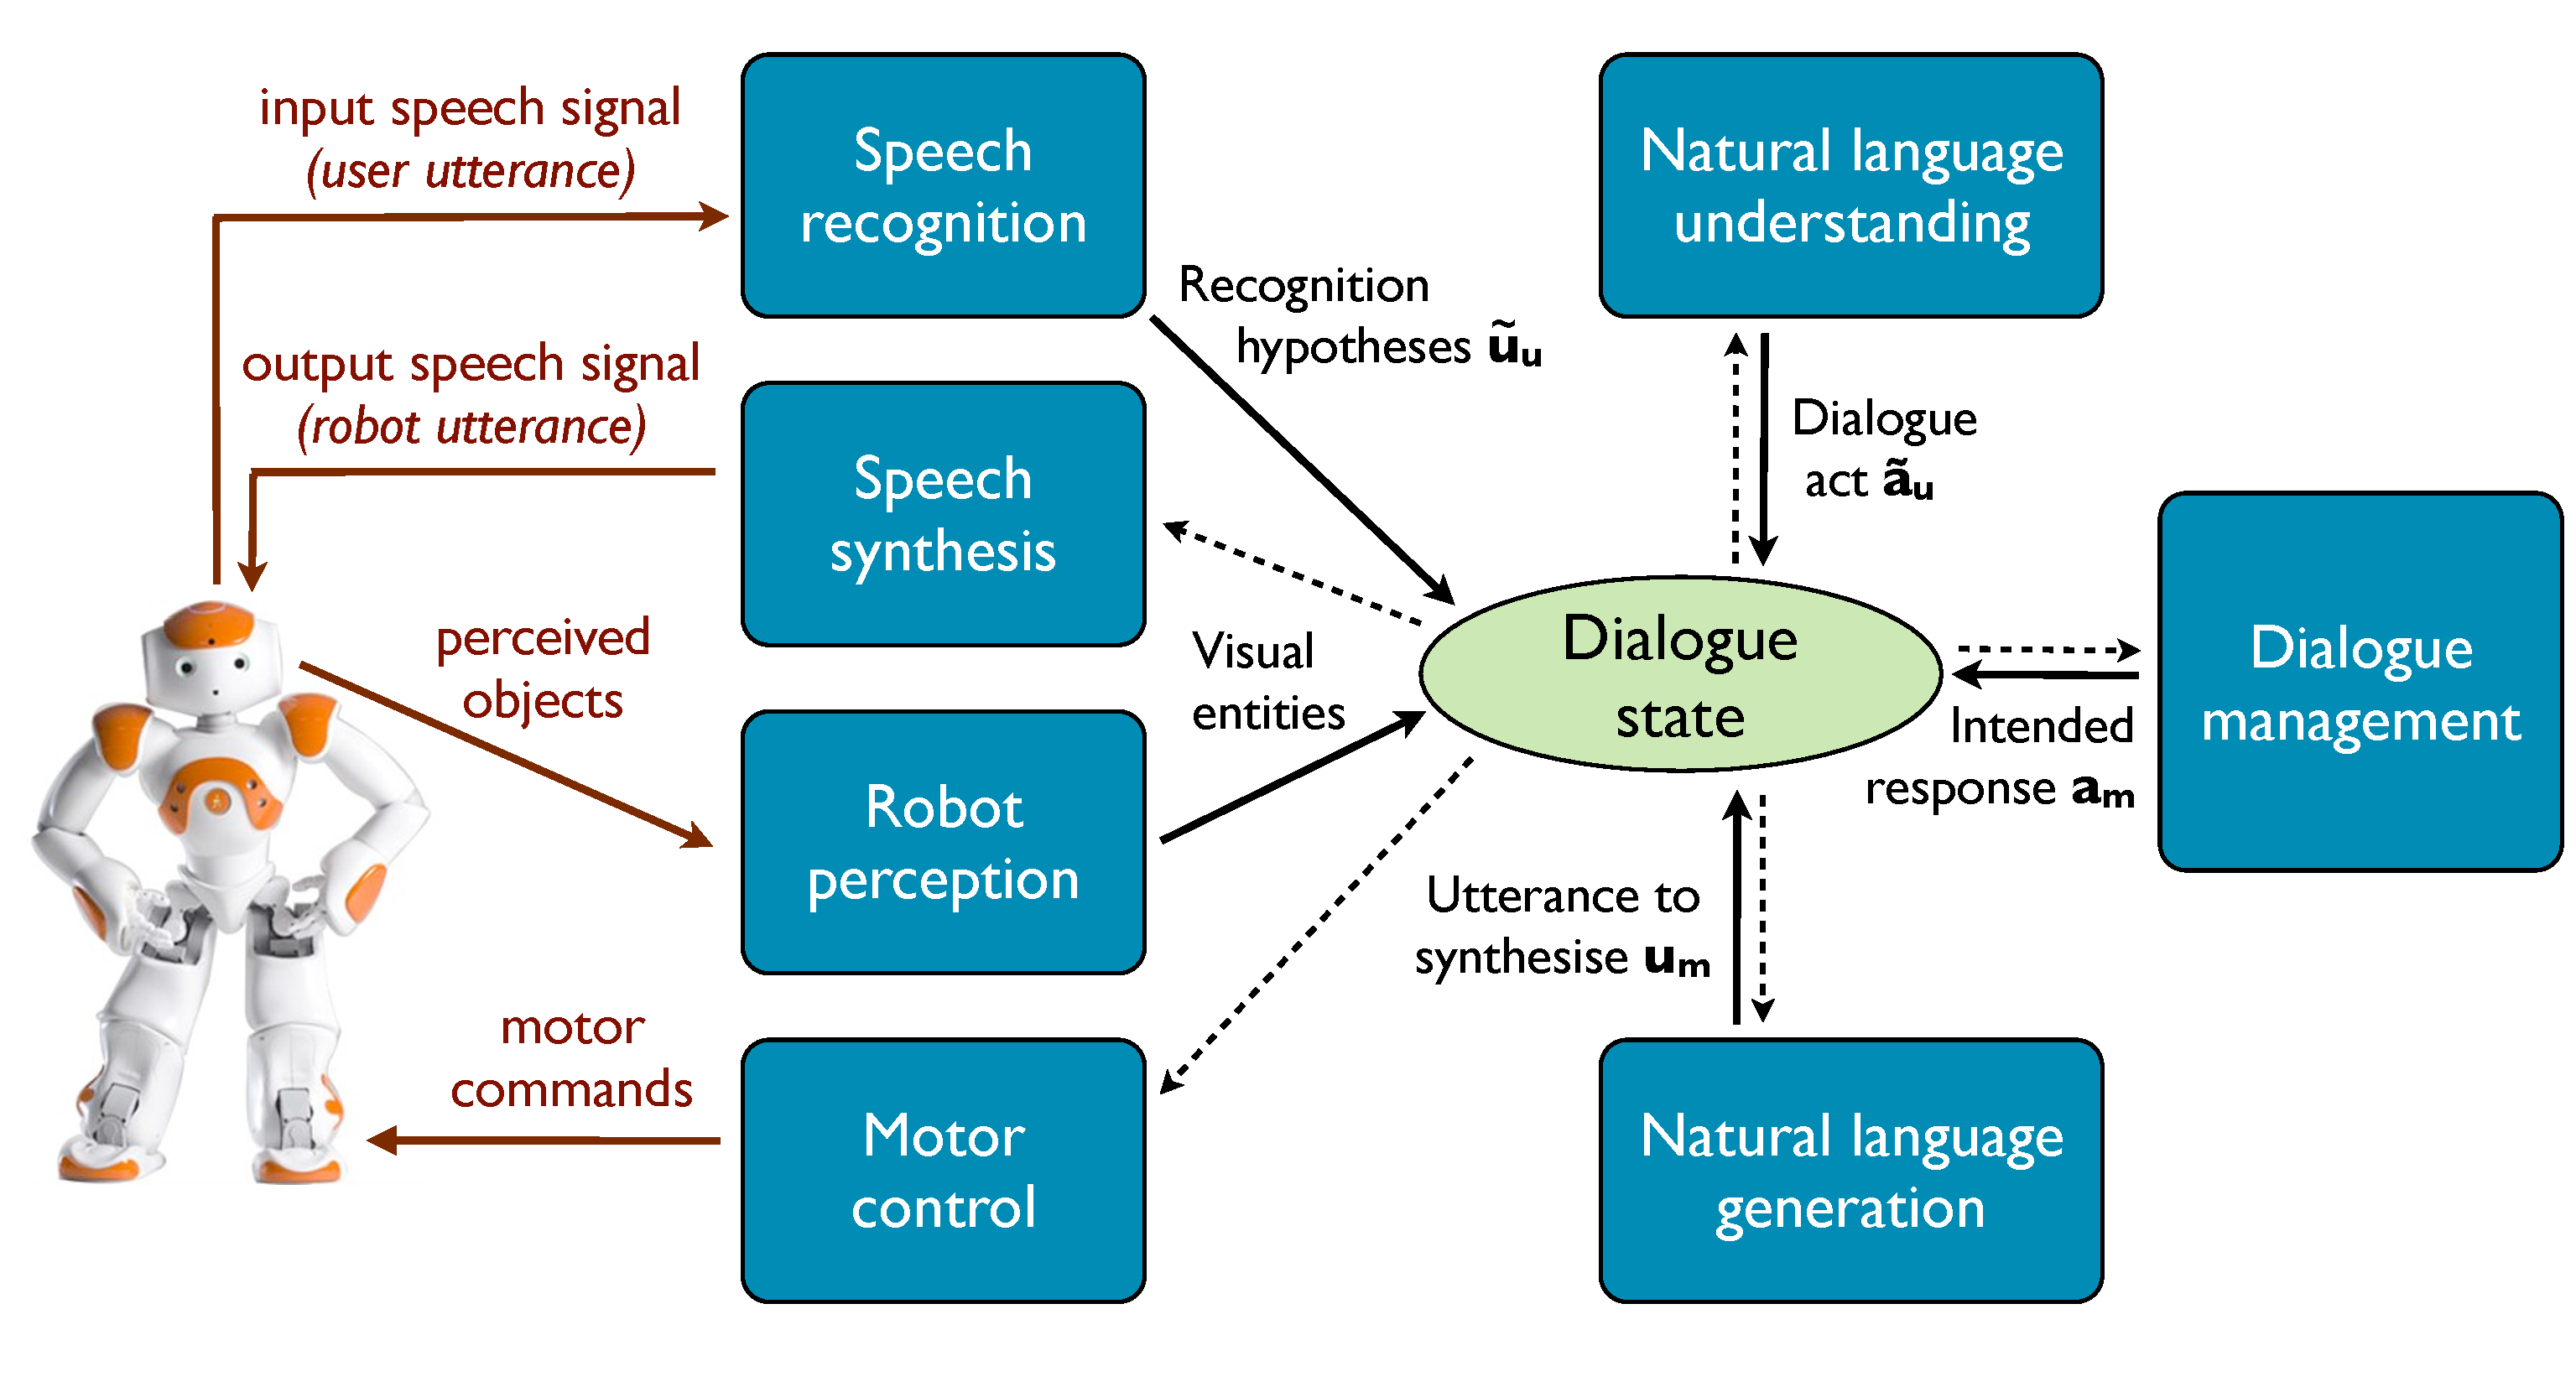
\includegraphics[scale=0.30]{imgs/impl_architecture.pdf}
\caption{Generic system architecture employed in the experiments.}
\label{fig:impl_architecture}
\end{figure}

The system modules can operate in either synchronous and asynchronous mode:\index{synchronous \& asynchronous processing} \begin{itemize}
\item Synchronous modules continuously monitor the dialogue state for relevant changes.  Their activation is thus performed in synchrony with the update events generated by the dialogue state.
\item Asynchronous modules run independently of the dialogue state.  They typically relate to visual or speech perception tasks. Asynchronous modules update the dialogue state as soon as new observations are made available. 

\end{itemize}

All modules have access to the complete dialogue state and can therefore exploit the full set of state variables (including generic contextual information) in their processing. 

\subsection{Individual modules}

We describe below the modules shown in Figure \ref{fig:impl_architecture} and explain their role and internal structure. It should be emphasised that the focus of the present thesis is on dialogue management.  The other system modules are therefore deliberately limited to simple, ``shallow'' processing methods in order to concentrate the implementation efforts on the dialogue manager. %Many of these modules could be extended to employ more sophisticated techniques, in particular in regard to speech recognition, natural language understanding and generation. 

\subsubsection*{Speech recognition}
\index{speech recognition}

Speech recognition is performed on the robot platform, using a commercial, off-the-shelf speech recognition engine (Vocon 3200 from Nuance).  Four microphones placed on the robot head are used for the sound capture.  The placement of the microphones on the robot allows the user to interact with the robot in a natural manner, without needing to resort to head-mounted microphones. This advantage comes, however, at the price of a lower sound quality due to the larger (and varying) distance between the sound source and the microphones.   This distance between source and receiver is indeed a major degradation factor in speech recognition \citep{wolfel2009distant}. Moreover, the microphones are also adjacent to a number of mechanical motors that may disturb the sound signal and lead to spurious detections.

The acoustic model\index{acoustic model} employed in all experiments is based on U.S. English. The language model\index{language model} takes the form of context-free recognition grammars in Bachus-Naur Form (BNF). Distinct grammars were used to cover the domain of discourse of each experiment. The grammars were designed by hand, based on the Wizard-of-Oz transcripts collected in our empirical studies (cf. previous chapters). Grammars can be dynamically attached or removed from the engine at runtime, thereby allowing the system to adapt the language model of the recogniser to the current dialogue context. Although this functionality is not directly exploited in the current implementation, we have shown in previous work \citep[see][]{ESSLLI2008-springerreprint} that such type of dynamic model adaptation\index{dynamic model adaptation} could lead to significant improvements in recognition accuracy for human--robot interaction settings, and would therefore constitute an interesting direction for the future development of the system.  As the recognition engine only generates hypotheses with raw, unnormalised confidence scores, a normalisation routine is used to convert them to proper probability distributions.\footnote{The conversion between confidence scores and probabilities is manually tuned in the current setup.  Future work may rely on more principled estimation techniques such as the ones outlined in \cite{Williams08}.}

%$P(\tilde{u}_u)$ 

\subsubsection*{Natural language understanding}
\index{natural language understanding}

The goal of natural language understanding (NLU) is to map a collection of utterance hypotheses $\tilde{u}_u$ to a corresponding set of dialogue act hypotheses $\tilde{a}_u$ expressing the semantic and pragmatic content of the user input. This understanding step is decomposed in our implementation in two tasks, dialogue act recognition and visual reference resolution.  

The goal of dialogue act recognition\index{dialogue acts!recognition of} is to construct the logical form representing the pragmatic meaning of the utterance. One should note that user utterances may contain more than one dialogue act, as for instance in \utt{yes and now pick the blue object} including both a backward-looking function (a confirmation) and a forward-looking function (a new instruction).  A collection of domain-specific templates was designed by hand to convert surface forms into logical representations of dialogue acts.  Although this approach does not allow for ``deep'' semantic extraction, it was shown to perform well in our dialogue domains. Future work may replace this template-based method with a data-driven semantic parser based on e.g.\  dependency parsing \citep{Nivre:Etal07}. \index{dependency parsing}

Reference resolution\index{reference resolution} is used to map linguistic expressions referring to objects in the visual context to their corresponding object identifier. The properties stated in the linguistic expressions are first matched against the set of possible references.  If the description remains ambiguous (i.e.\ more than one object matches the linguistic expression), the references can be further ranked according to their visual saliency, defined in terms of their physical distance to the robot.  The pronoun \utt{it} is resolved by searching for the closest object reference in the dialogue history. 

Natural language understanding is practically implemented in \opendial{} via probabilistic rules.  As seen in Section \ref{sec:amodelling}, the formalism of probabilistic rules already includes special-purpose operators for string manipulation and can thus readily encode the shallow templates\index{shallow template} used for dialogue act recognition.  Rule $r_{15}$ below is an example of such a rule.  The rule lists three regular expression patterns associated with the dialogue act $\mathrm{MoveArm(Left,Down)}$.  If the value for the user utterance variable $u_u$ matches at least one of the patterns, the dialogue act $a_u$ is classified as $\mathrm{MoveArm(Left,Down)}$:
\begin{align*}
r_{15}: &\;\;\textbf{if} \ (u_u \textit{ matches } \text{``(*) left arm down''} ) \\ 
& \lor (u_u \textit{ matches } \text{``(*) lower (the\,|\,your) left arm''} ) \\
& \lor (u_u \textit{ matches } \text{``(*) down (the\,|\,your) left arm''}   )  \ \ \textbf{then} \\ 
& \; \; \begin{cases} P\left(a_u' = \mathrm{MoveArm(Left,Down)}\right) = 1.0 \end{cases}
\end{align*}

\subsubsection*{Dialogue management}

Dialogue management\index{dialogue management} follows the procedure outlined in the previous chapters and will not be repeated here. For each update of the dialogue state, the dialogue manager triggers the corresponding rule-structured models, and selects the next action to perform (if any). 

\subsubsection*{Natural language generation}
\index{natural language generation}

If the system action selected by the dialogue manager is non-empty and denotes a verbal action, the natural language generation module is triggered.  As for natural language understanding, the generation component of \opendial{} is based on a manually designed collection of templates.  The processing direction is the reverse of natural language understanding, as the templates are applied to convert a logical representation of the communicative goal into a surface form. 

The generation templates are also encoded with a rule-structured model.  The rules correspond here to utility rules, since natural language generation is at its core a decision-making task corresponding to the choice of a particular linguistic realisation for the intended communicative goal.  As an example, rule $r_{16}$ generates the system response $u_m$ given the system act $a_m=\mathrm{Acknowledgement}$.  The rule specifies in this case three alternatives with equal utility:
\begin{align*}
r_{16}: &\;\;\textbf{if} \ (a_m = \mathrm{Acknowledgement} )  \ \ \textbf{then} \\ 
& \;\; \begin{cases} U(u_m'=\text{``ok''}) = 1 \\ U(u_m=\text{``great''}) = 1 \\ U(u_m'=\text{``thanks''}) = 1 \end{cases}
\end{align*}

The presence of multiple realisations allows for some variation in the system behaviour, since the system will automatically select one realisation at random due to the uniform utility assigned to the alternative realisations.

\subsubsection*{Speech synthesis}
\index{speech synthesis}

Speech synthesis is performed on the robot, using an off-the-shelf speech synthesis engine developed by Acapela\footnote{\begin{scriptsize}\url{http://www.acapela-group.com}\end{scriptsize}}. The synthesis engine is based on unit selection. The output speech signal is then sent to two speakers placed on the robot head. To avoid spurious recognition results, the speech recognition is automatically disabled when the robot is speaking.  
 
\subsubsection*{Robot perception}
\index{robot perception}

The robot can detect simple physical objects present in the visual scene. The object detection is done based on the vision libraries bundled with the robotic platform. Special  markings are placed on top of the objects to facilitate the object recognition and the visual servoing.  

\subsubsection*{Robot motion control}
\index{motion control}

Various types of physical movements were engineered for the purpose of our experiments, including: \begin{itemize}
\item generic body movements: rotating the arms and the head in various directions,
\item spatial navigation: moving forward and backward, turning left and right,
\item object manipulation: grasping and releasing objects.  
\end{itemize}

All the movements were programmed using the motion control libraries available on the robot. The object manipulation relies on the use of permanent magnets attached to the robot hands. 


\subsection{Graphical interface}
\index{graphical user interface}

The graphical user interface developed for the \opendial{} toolkit enables the system designer to monitor and control in real-time the state of the system.  The interface is divided in two  views, shown as distinct tabs in the application window: the chat window and the dialogue state monitor.

\subsubsection*{Chat window}
\index{chat window}

The main user interface displays the interaction history as a chat window, as illustrated by the screen capture in Figure \ref{fig:gui-chatbox}.


\begin{figure}[ht]
\centering
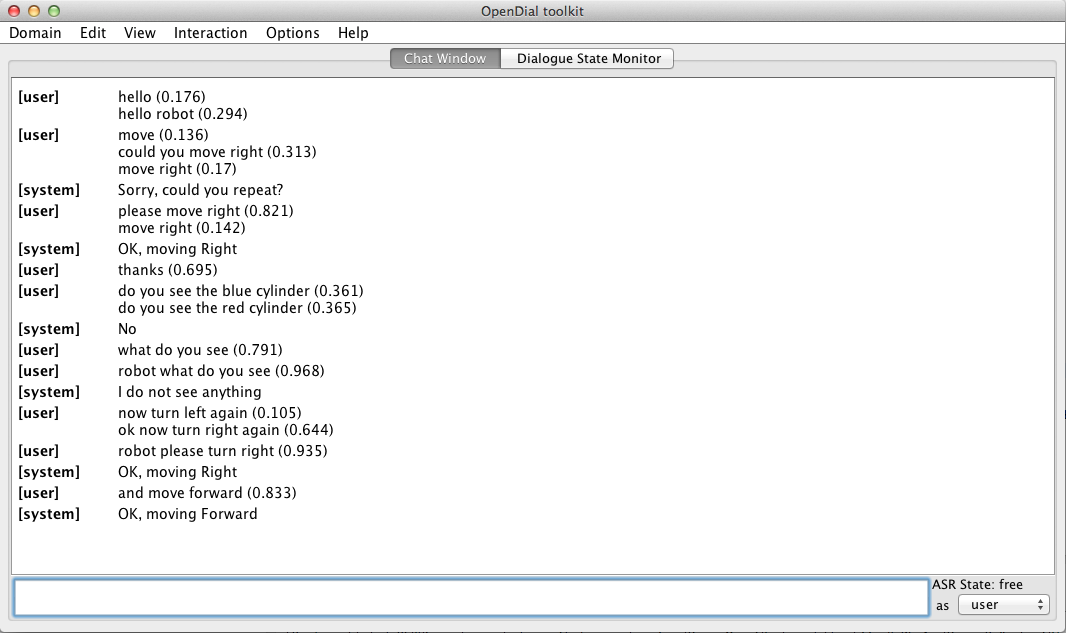
\includegraphics[scale=0.40]{imgs/gui-chatbox.png}
\caption{Graphical user interface showing the interaction history.}
\label{fig:gui-chatbox}
\end{figure}

  The user inputs are displayed as N-best lists together with their corresponding probabilities. In addition to monitoring the interaction, the chat window can also be used to test the dialogue system by typing new user and system inputs in the input field at the bottom of the window.  A drop-down field in the button right corner is used to switch the agent role (e.g.\ for Wizard-of-Oz experiments). 


\subsubsection*{Dialogue state monitor}
\index{dialogue state monitor}

To allow the system designer to easily inspect the content of the dialogue state, a state visualisation tool has also been integrated into \opendial{}.  The monitor provides a visual representation of the dialogue state in the form of a directed graph with nodes corresponding to the state variables and directed edges corresponding to conditional dependencies.\footnote{The graphs are rendered with JUNG, an open source toolkit for drawing graphs: \begin{scriptsize}\url{http://jung.sourceforge.net}\end{scriptsize}.} An example of a graph layout is shown in Figure \ref{fig:gui-bn}. The graph is dynamically refreshed after each update of the dialogue state, using standard graph drawing algorithms to optimise the layout of nodes on the screen. 

In addition to depicting the current dialogue state, the monitor also records and stores previous dialogue states.  The dialogue state to visualise can be selected among the list on the left side of the window. This functionality is particularly useful to compare dialogue states with one another and analyse how the dialogue state is evolving over time. 

\begin{figure}[p!] 
\begin{center}
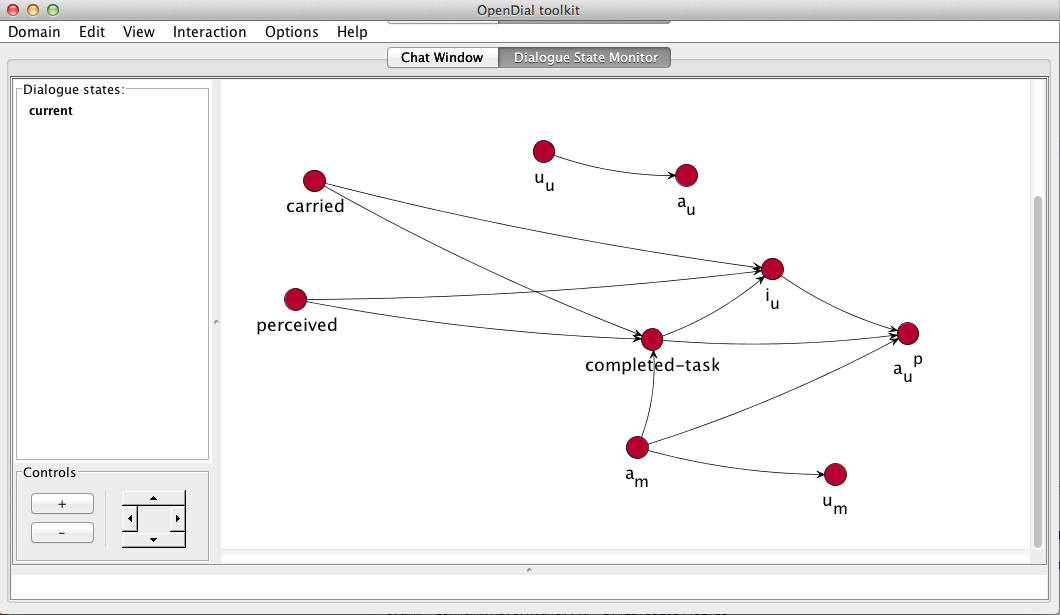
\includegraphics[scale=0.40]{imgs/gui-bn.png}
\end{center} 
\caption{Visualisation of the current dialogue state.}
\label{fig:gui-bn}
\end{figure}

\begin{figure}[p!] 
\begin{center}
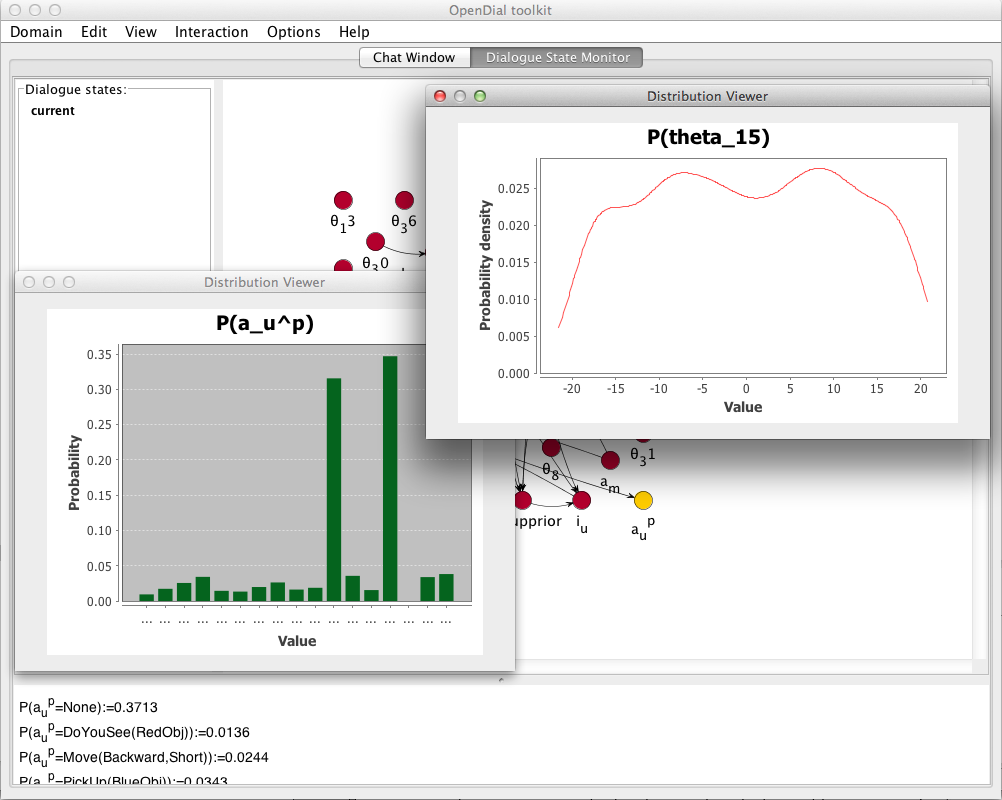
\includegraphics[scale=0.40]{imgs/gui-distribviewer.png}
\end{center} 
\caption{Visualisation of a discrete probability distribution $P(a_u^p)$ and a continuous probability distribution $P(\theta_{15})$ in the dialogue state monitor.}
\label{fig:gui-distribviewer}
\end{figure}

The user can manipulate the graph in multiple ways in order to e.g.\ analyse the content of specific state variables, add or remove evidence, or request the calculation of marginal distributions on selected set of variables.  The inference results are in this case shown in the text area at the bottom of the window.  In addition, the system designer can also zoom in on selected probability distributions using the distribution viewer tool illustrated in Figure \ref{fig:gui-distribviewer}. Discrete probability distributions are shown as histograms, while continuous probability distributions are represented by their probability density functions.\footnote{The probability distributions are rendered with the open source toolkit JFreeChart: \begin{scriptsize}\url{http://jfreechart.sourceforge.net}\end{scriptsize}.} 


\section{Conclusion}

This chapter exposed the practical integration of our structured modelling framework in the \opendial{} toolkit and its instantiation in a spoken dialogue system for human--robot interaction. The first section presented the general architecture of the toolkit, the declarative specification of dialogue domains in an XML format, and the implementation of efficient algorithms for inference, sampling and planning. We notably discussed the benefits of using a shared description formalism in terms of transparency, portability, flexibility and adaptivity over traditional ``black-box'' architectures. We also compared \opendial{} to other existing architectures and pointed out a number of limitations in the current implementation of the toolkit, such as its lack of incremental processing and its limited turn-taking behaviour. 

The \opendial{} toolkit is inspired by both symbolic and statistical approaches to dialogue, and combines an information state architecture with probabilistic reasoning based on rule-structured models.  As stated in the introduction chapter, the long-term goal of the \opendial{} framework is to bridge the gap between symbolic approaches to dialogue management, which usually concentrate on capturing rich interaction patterns, and probabilistic approaches, more focused on aspects related to noise, uncertainty, and adaptivity. 

The hybrid design  of \opendial{} allows system designers to exploit powerful generalisations in the dialogue domain specification without sacrificing the probabilistic nature of the model. Another important side benefit of probabilistic rules is their improved readability for human experts, which are able to leverage their domain knowledge in the form of pragmatic rules, common sense assumptions, or task-specific constraints. Furthermore, the internal organisation of rules into models enables dialogue domains to be specified in a modular fashion, by clustering rules into distinct models.  Some models may therefore reflect highly domain-specific knowledge while others encode generic interaction patterns that can easily be ported to other applications.  

The last section described the integrated dialogue system used to carry out the practical experiments presented in Chapters \ref{chap:wozlearning}, \ref{chap:rllearning} and \ref{chap:user-evaluation}.  The system comprised both synchronous and asynchronous components and included dedicated modules for speech recognition, speech synthesis, robot perception and motor control.  Natural language understanding, dialogue management and natural language generation were encoded with models structured with probability rules. 

The next chapter demonstrates the practical deployment of this system in a full-scale user evaluation study. 

\bibliography{lt-biblio}

\printindex

\end{document}
